\glsresetall
\newcommand{\acem}{\acrshort{cem}\xspace}
\newcommand{\ce}{{\ensuremath{\text{CE}}}}
\newcommand{\pce}{{\ensuremath{\psi_{\text{CE}}}}}
\newcommand{\hpce}{{\ensuremath{\hat\psi_{\text{CE}}}}}

\newcommand{\aeis}{\acrshort{eis}\xspace}
\newcommand{\eis}{{\ensuremath{\text{EIS}}}}
\newcommand{\peis}{{\ensuremath{\psi_{\text{EIS}}}}}
\newcommand{\hpeis}{{\ensuremath{\hat\psi_{\text{EIS}}}}}

\newcommand{\Pp}{{\ensuremath{\mathbb P^{X| Y=y}}}}
\newcommand{\Pps}{{\ensuremath{\mathbb P^{S| Y=y}}}}

\newcommand{\la}{{\ensuremath{\text{LA}}}}

\newcommand{\Dto}{\stackrel{\mathcal D}{\to}}
\newcommand{\id}{\operatorname{id}}


\newcommand{\nbinom}{\operatorname{NegBinom}}
\newcommand{\bdiag}{\operatorname{block-diag}}

\chapter{Importance Sampling in State Space Models}
\label{cha:state_space_models}
\newpage
\begin{tcolorbox}[title={Contributions}]
    The main contribution of this chapter consists of a rigorous comparison of two importance sampling frameworks: the \Acrfull{cem} and \Acrfull{eis}. Both methods determine optimal importance sampling proposals, but have, until now, been studied in separate communities: the \acem is popular in rare-event estimation and engineering disciplines, while \aeis is popular in the financial time series community. 

    The contributions of the individual sections are as follows:

    %\paragraph{\nameref{sec:modelling_epidemiological_dessiderata_with_state_space_models}} 

    \paragraph{\nameref{sec:linear_gaussian_state_space_models}} This section is loosely based on \citep{Durbin2012Time}.
    \paragraph{\nameref{sec:logconcave_gaussian_state_space_models}} This section is loosely based on \citep{Durbin2012Time,Brown1986Fundamentals}.
    \paragraph{\nameref{sec:importance_sampling}} While the general treatment of importance sampling is based on \citep{Chopin2020Introduction,Durbin2012Time}, we contribute the following:
    \begin{itemize}
        \item We prove \Cref{lem:bounded-log-variance} and \Cref{cor:dkl_bounded}.
        \item Discussion surrounding \Cref{thm:chatterje2018Thm1}, especially \Cref{ex:ess_failure}.
        \item The analysis of asymptotics of importance sampling methods, i.e. \Cref{prop:is-consistency,prop:is-clt}.
        \item The consistency and CLT results for the \acrshort{cem} (\Cref{thm:cem-consistent,thm:cem-clt}) and \acrshort{eis} (\Cref{thm:eis-consistent,thm:eis-clt}).
        \item The discussion of assumptions required in the CLTs for practical applications.
    \end{itemize}

    \paragraph{\nameref{sec:interim-discussion}}
    The whole section is newly contributed.

    \paragraph{\nameref{sec:gaussian_importance_sampling_for_state_space_models}}
    \begin{itemize}
        \item The discussion surrounding the difficulties the \acrshort{cem} faces when applied to the \acrshort{glssm} proposal.
        \item The derivation of the \acrshort{cem} for Markov-proposals (\Cref{prop:cem-for-markov-proposal}), resulting in \Cref{alg:cem-markov-proposal} and the optimized \Cref{alg:cem-markov-proposal-fast}.
    \end{itemize}

    \paragraph{\nameref{sec:maximum_likelihood_estimation}}
    This section is for the largest part based on literature, however the following points are new:
    \begin{itemize}
        \item The discussion of calculating the gradient, \Cref{eq:gradient_infeasible}, for the \acrshort{la} / \acrshort{eis}.
        \item We make the antithetic variable construction of \citep{Durbin1997Monte} rigorous. 
        \item \Cref{subsec:inference} is a rigorous reformulation of \citep[Section 11.5]{Durbin2012Time}.
    \end{itemize}

    \paragraph{\nameref{sec:simulation_studies}} 
    This whole section is a new contribution, extensively comparing the \acrshort{cem} with \acrshort{eis}.
\end{tcolorbox}
\newpage

In the last chapter, we have detailed the need for models capable of modeling complex epidemiological phenomena. Crucially, we must account for the time-series and discrete nature of the data at hand. 
\Glspl{ssm} form a versatile class of statistical models that allow modeling of non-stationary time series data while providing a straightforward, mechanistic interpretation of the time series' dynamics.
The main idea of these models is to introduce unobserved \textbf{latent states} whose joint distribution is governed by a Markov process, and to model the observed time series conditional on these states.
By exploiting this structure, inference in \glspl{ssm} becomes computationally efficient, as the complexity of algorithms is linear in the number $n$ of time points considered. 
In this chapter, we provide a mathematical introduction to the theory of \acrshortpl{ssm} and the main tool we will use for inference: importance sampling. 
%Additionally, we will highlight how to use \acrshortpl{ssm} to model the desiderata identified in \Cref{sec:dessiderata}. 
The foundations of \acrshortpl{ssm} presented in this chapter are, if not mentioned otherwise, based on \citep{Durbin2012Time,Chopin2020Introduction}.

Let us start from a very general definition of a \acrshort{ssm}.

\begin{definition}[State Space Model]
    \label{def:ssm}
    A \textbf{\acrlong{ssm}} is a discrete time stochastic process $(X_t, Y_t)_{t=0, \dots, n}$ taking values in the measurable space $\left(\mathcal X \times \mathcal Y, \mathcal B_{\mathcal X} \otimes \mathcal B_{\mathcal Y}\right)$ such that
    \begin{enumerate}
        \item The marginal distribution of the \textbf{states} $(X_0, \dots, X_{n})$ is a discrete time Markov process, i.e. for $t = 1, \dots, n$
              \begin{align}
                  \label{eq:markov_property}
                  \P \left( X_{t} \in B \middle| X_0, \dots, X_{t - 1} \right) = \P \left( X_{t} \in B \middle| X_{t - 1} \right) \text{ a.s.}
              \end{align}
              for all measurable $B \in \mathcal B_{\mathcal X}$.
        \item Conditional on the state $X_t$ and observation $Y_{t - 1}$, $Y_t$ is independent of $X_s$ and $Y_{s - 1}$, $s < t$, i.e.
              \begin{align*}
                  \P \left( Y_{t} \in B \middle| X_{0}, \dots, X_{t}, Y_{0}, \dots, Y_{t - 1} \right) & = \P \left( Y_{t} \in B | X_{t}, Y_{t - 1} \right)
              \end{align*}
              for all measurable $B \in \mathcal B _{\mathcal Y}$.
    \end{enumerate}
\end{definition}

For notational convenience, we will write $\gls{sym:Xs-to-t} = \left(X_s, \dots, X_{t}\right)$ for the vector that contains all states from $s$ to $t$, $s \leq t$, dropping the first index if we consider the whole set of observations up to time $t$, so $\gls{sym:X-to-t} = X_{0:t}$, and dropping the subscript if we consider all states at once, $X = X_{:n}$.
Similarly we set $Y_{s:t} = \left(Y_s, \dots, Y_{t}\right)$, $Y_{:t} = Y_{0:t}$ and $Y = Y_{:n}$.

The models that we consider in this thesis will usually assume that densities for the state transitions with respect to a common dominating measure $\mu_{\mathcal X}$ and similar for the observations with respect to some dominating measure $\mu_{\mathcal Y}$ exist. 

\begin{notation}[Densities, conditional densities]
    \label{not:densities}
    We will use the standard abuse of notation for densities that makes the type of density ``{}obvious''{} from the arguments used.
    This means that $\gls{sym:p}(x)$ is the density for all states $X$, evaluated at $x$, $p(x_t|x_{t - 1})$ the conditional density of $X_t|X_{t - 1}$, evaluated at $x_{t}$ and $x_{t - 1}$ and similarly for observations: $p(y|x)$ is the density of the conditional distribution of all observations $Y$ conditioned on all states $X$, evaluated at $y$ and $x$.

    Note that this notation also implicitly includes the time $t$ and allows for changes in, e.g., the state transition over time.

    When densities come from a parametric model parametrized by $\gls{sym:theta}\in \gls{sym:Theta} \subseteq \mathbf{R}^{l}$ and the dependence of the model on $\theta$ is of interest, e.g. because we try to estimate $\theta$, we indicate this by adding a subscript to the densities.
    If this dependence is not of interest, e.g. because $\theta$ is fixed, we omit $\theta$ for better readability.

    In this notation, the joint density of a parametric \gls{ssm} factorizes as
    \begin{align}
        \label{eq:joint_density}
        \begin{split}
        p_\theta(x,y) & = p_\theta(x_0, \dots, x_{n}, y_0, \dots, y_{n})                                                              \\
                      & = p_\theta (x_0)\prod_{t = 1}^{n} p_\theta(x_{t}|x_{t - 1}) \prod_{t = 0}^{n} p_\theta(y_t | x_t, y_{t - 1}),
        \end{split}
    \end{align}
    where $p_\theta(y_0|x_0, y_{-1}) = p_\theta(y_0| x_0)$.

    As inferences made in this thesis depend on the \gls{ssm} only through the likelihood we identify almost sure versions of $(X, Y)$ with themselves, i.e. all equations involving $X$ or $Y$ are understood almost surely.
\end{notation}

\begin{remark}[dependence on $Y_{t - 1}$, dimensions]
    \label{rem:dependence_Yt-1}
    Contrary to the standard definition of a \gls{ssm}, as found in, e.g., \citep[Chapter 2]{Chopin2020Introduction} or \citep[Chapter 9]{Durbin2012Time}, our \Cref{def:ssm} allows $Y_t$ to depend on $Y_{t - 1}$.
    As the models considered in \Cref{cha:analysis_of_selected_models} will make extensive use of \glspl{ssm} with this dependency structure we opt to use this non-standard definition here.
    This is of course not a limitation of the standard definition: given a \gls{ssm} of the form described in \Cref{def:ssm}, we can transform it to the standard form by choosing states $(X_t, Y_t) \in \mathcal X \times \mathcal Y$ and observations $Y_t \in \mathcal Y$ such that the \gls{ssm} becomes a stochastic process on $ \left( \mathcal X \times \mathcal Y\right) \times \mathcal Y$.

    Additionally, the goal of our inferences will always be functionals of the conditional distribution $X|Y$ for a single, fixed, set of observations $y$. Assuming all densities exist, the conditional density $p(x|y)$ is given, up to a constant not depending on $x$, by \Cref{eq:joint_density}:
    $$
    p(x|y) \propto p(x,y) =p (x_0)\prod_{t = 1}^{n} p(x_{t}|x_{t - 1}) \prod_{t = 0}^{n} p(y_t | x_t, y_{t - 1}).
    $$
    Thus, the dependence of $Y_{t}$ on $Y_{t - 1}$ only affects our inferences through $p(y_{t} | x_{t}, y_{t - 1})$, where, as $Y_{t - 1}$ is observed, the argument $y_{t - 1}$ is fixed. By a similar argument, we could allow $Y_{t}$ to depend on all previous observations $Y_{0}, \dots, Y_{t - 1}$ without changing any of our inferences. However, the models presented in \Cref{cha:analysis_of_selected_models} will not make use of this further generalization.
    Consequently, all results we present in this chapter for \acrshortpl{ssm} where $Y_{t}$ depends only on $X_{t}$ that concern only the conditional distribution $X|Y=y$ carry over to those given by \Cref{def:ssm}. We will reiterate this argument at appropriate points in this thesis.

    In most \acrshortpl{ssm} we consider in this thesis we use $\mathcal X = \R^m$ and $\mathcal Y = \R^p$ or $\mathcal Y = \Z^p$ so that $\mathcal X$ is $m$ dimensional and $\mathcal Y$ is $p$ dimensional and equip these spaces with the usual $\sigma$-Algebras. Unless noted otherwise, we use for $\mu_{\mathcal X}$ the $m$-dimensional Lebesgue measure and for $\mu_{\mathcal Y}$ either the $p$-dimensional Lebesgue measure ($\mathcal Y = \R^{p}$) or the $p$-dimensional counting measure ($\mathcal Y = \Z^{p}$).
    
\end{remark}

\begin{figure}
    \centering
    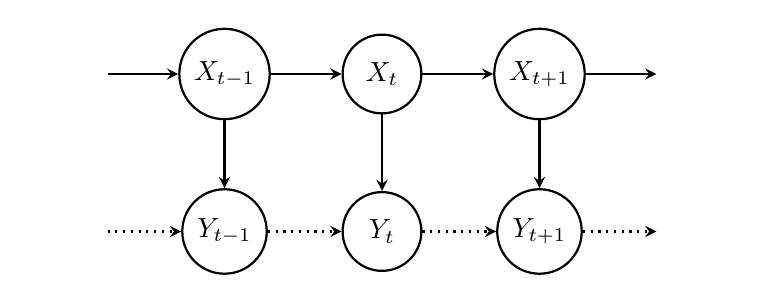
\begin{tikzpicture}[->, >=stealth, thick, node distance=2cm, every node/.style={circle, draw, minimum size=1cm}]

    % empty nodes 
    \node[draw=none] (Xtm2) at (-4,2) {};
    \node[draw=none] (Xtp2) at (4,2) {};
    \node[draw=none] (Ytm2) at (-4,0) {};
    \node[draw=none] (Ytp2) at (4,0) {};

    % Nodes for X_t
    \node (Xtm1) at (-2,2) {$X_{t-1}$};
    \node (Xt) at (0,2) {$X_t$};
    \node (Xtp1) at (2,2) {$X_{t+1}$};

    % Nodes for Y_t
    \node (Ytm1) at (-2,0) {$Y_{t-1}$};
    \node (Yt) at (0,0) {$Y_t$};
    \node (Ytp1) at (2,0) {$Y_{t+1}$};

    % Arrows for X_t dependencies
    \draw[thick] (Xtm2) -- (Xtm1);
    \draw[thick] (Xtm1) -- (Xt);
    \draw[thick] (Xt) -- (Xtp1);
    \draw[thick] (Xtp1) -- (Xtp2);

    % Arrows for Y_t dependencies
    \draw[thick] (Xtm1) -- (Ytm1);
    \draw[thick] (Xt) -- (Yt);
    \draw[thick] (Xtp1) -- (Ytp1);

    % Dotted arrow for Y_t-1 to Y_t
    \draw[dotted, thick] (Ytm2) -- (Ytm1);
    \draw[dotted, thick] (Ytm1) -- (Yt);
    \draw[dotted, thick] (Yt) -- (Ytp1);
    \draw[dotted, thick] (Ytp1) -- (Ytp2);

\end{tikzpicture}
%
    \caption{Dependency structure in a \acrshort{ssm} as given by \Cref{def:ssm}. The dependencies between observations $Y_{t-1}$ (indicated by dotted arrows) are usually not part of the standard definition of a \acrshort{ssm}, but can be incorporated in a straightforward manner.}
    \label{fig:ssm_dependencies}
\end{figure}


Given data $y = (y_t)_{t = 0, \dots, n}$ that may be modeled with a \gls{ssm} the practitioner is confronted with several tasks, which provide the structure of this chapter:

\begin{enumerate}
    \item\label{it:model_choice} Choosing a suitable, usually parametric, class of \glspl{ssm} that include the effects of interest.
    \item\label{it:model_fitting} Fitting such a parametric model to the data at hand by either frequentist or Bayesian techniques.
    \item\label{it:smoothing_problem} Infer the latent states $X$ from the observations by determining, either analytically or through simulation, the smoothing distribution $X|Y$.
\end{enumerate}

The first step, \cref{it:model_choice}, requires that the practitioner specifies a joint probability distribution for the states and observations (see \Cref{cha:analysis_of_selected_models} for examples of this).
Due to the assumed dependency structure, this boils down to specifying transition kernels for the states and observations.
The setting given in \Cref{def:ssm} is too abstract to perform inference in, so further assumptions on the types of distributions for the latent states and observations are needed.
In this chapter, we will discuss \glspl{glssm}  (\Cref{sec:linear_gaussian_state_space_models}), where both the posterior distribution and the likelihood can be derived analytically. For the epidemiological application we have in mind, these are, however, insufficient due to the non-linear behavior of incidences and the low count per region (\Cref{sec:dessiderata}).
Such observations are better modeled with distributions on the natural numbers, i.e. with a Poisson or negative binomial distribution, both of which are exponential families of distributions. This will lead to the class of \acrfullpl{pgssm} (\Cref{sec:logconcave_gaussian_state_space_models}) which will become the main focus of our study.

Regarding the second step, \cref{it:model_fitting}, a frequentist practitioner will want to perform maximum likelihood inference on $\theta$.
While asymptotic confidence intervals for the \gls{mle} $\hat\theta$ can be derived both theoretically and practically \citep[Chapter 7]{Durbin2012Time}, they are, in the context of this thesis, usually of little interest. For these asymptotic frequentist procedures to be meaningful, an appropriate central limit theorem must hold. However, as the time series we study are non-stationary and the dependence on parameters $\theta$ is allowed to be arbitrary, it is in general not obvious that such a theorem holds for the model under consideration. Instead, we approach this fitting as an Empirical Bayes procedure and our main practical interest lies in analyzing the posterior distribution $X|Y$ where we set $\theta$ equal to $\hat\theta$. 


To obtain the maximum likelihood estimates $\hat\theta$ one needs access to the likelihood
\begin{align}
    \label{eq:likelihood}
    p_{\theta}(y) = \int_{\mathcal X^{(n + 1)}} p_{\theta}(x,y) \d (\mu_{\mathcal X})^{(n+1)}x =\int_{\mathcal X^{(n + 1)}} p_{\theta}(x,y) \d x = \int_{\mathcal X^{(n + 1)}} p_{\theta}(y|x) p_{\theta}(x) \d x
\end{align}
which is usually not analytically available. Here and in the following we assume that $\mathcal X = \R^{m}$ for some $m \in \N$, that $p$ is absolutely continuous with respect to the $m$-dimensional Lebesgue measure and that $p$ is regular enough that the integral is a Riemann integral.
Direct numerical evaluation of \Cref{eq:likelihood} is hopeless due to the high dimensionality of the state space $\mathcal X^n$.
Instead, we will resort to simulation-based inference by importance sampling (see \Cref{sec:importance_sampling}), a Monte-Carlo method that approximates $p(y)$ by constructing a global tractable approximation to the integrand in \Cref{eq:likelihood}. Alternatively, \gls{smc} methods, i.e. particle filters, that perform importance sampling sequentially across the $n + 1$ time steps can be used. We will not follow this approach for reasons described later, but refer the reader to the excellent reference \citep{Chopin2020Introduction} for an introduction to these methods.

The performance of such simulation-based estimates depends crucially on our ability to construct distributions that are close to the posterior $p(x|y)$ but are easy to sample from. To this end, we construct either \acrfullpl{glssm} (\Cref{subsec:glssm-approach}) in which sampling from the posterior is analytically possible, or Gaussian Markov processes (\Cref{subsec:markov-approach}) which are directly amenable to simulation.
These two approaches are motivated by what we term ``{}optimal importance sampling''{}, where we use a proposal distribution that solves an optimization problem. Two popular approaches for choosing such a proposal are \acrlong{eis} and the \acrlong{cem}, which minimize an $L^{2}$ or \acrshort{kld} loss, respectively. Empirically, it has been shown that \acrshort{eis} outperforms the \acrshort{cem}, to which we add theoretical insight in the form of two central limit theorems (\Cref{sec:importance_sampling}): as both methods rely on importance sampling to determine an optimal proposal, the asymptotic variance of this procedure is of practical relevance, and we argue that this asymptotic variance is typically smaller for \acrshort{eis}.
To this end, we provide extensive simulation studies investigating the asymptotic variance of the two methods in \Cref{sec:simulation_studies}. 
To the best of the authors' knowledge, this is the first rigorous investigation comparing these two methods. 
%This will be a good strategy if the target posterior $p(x|y)$ can be well approximated by a Gaussian distribution --- otherwise, we may want to account for multiple modes by considering mixtures of Gaussian state space models or account for heavy tails with t-distributed errors (\Cref{sec:accouting_for_multimodality_and_heavy_tails}) \todo{keep this here?}.

Finally, \cref{it:smoothing_problem} concerns the actual inference of the latent states $X$ given observations $Y=y$, a classical problem in Bayesian inference. Except for the \acrshort{glssm} (\Cref{sec:linear_gaussian_state_space_models}), the posterior distribution $X|Y=y$ is usually not analytically tractable, and we have to resort to simulation-based methods. We favor importance sampling over \gls{mcmc} methods due to the ease of implementation and the possibility to parallelize the simulations.

As an alternative to the above, \acrshort{mle}-based approach, a fully Bayesian approach would regard $\theta$ as random and administer a prior distribution, say with density $p(\theta)$. In this setting, the main interest still lies in determining the posterior distribution of $X|Y=y$, but due to the prior put on $\theta$, its density, should it exist, is now given by
$$
p(x|y) = \int p(x,\theta|y) \d \theta,
$$
where $p(x,\theta|y)$ is the joint posterior of states and hyperparameters, conditional on observations $y$. To tackle this problem, one may again use importance sampling methods, see e.g. \citep[Chapter 13.1]{Durbin2012Time}, or use \acrshort{mcmc}-methods tailored to \acrshortpl{ssm}, e.g. Particle-\acrshort{mcmc} \citep[Chapter 16]{Chopin2020Introduction} --- however this approach is outside the scope of this thesis.


To perform the above tasks, the setting defined in \Cref{def:ssm} is too general to have numerically tractable solutions. Thus we restrict our studies to more structured \acrshortpl{ssm}. We begin with assuming a joint Gaussian distribution for states and observations. Subsequently, we will relax this assumption to allow the observations $Y$ to have more general distributions. 
%
\section{Modeling epidemiological desiderata with state space models}
\label{sec:modelling_epidemiological_dessiderata_with_state_space_models}
\todo{find place for this paragraph}
The Poisson distribution arises from the law of small numbers: if there is a large population where every individual has, independently, a small probability of becoming infected in a small window of time then the total number of infections in that window of time is well approximated by the Poisson distribution.
Indeed, the law of small numbers remains valid for small dependencies \citep{Ross2011Fundamentalsa,Arratia1990Poisson}.
However, incidences observed from the SARS-CoV-2 epidemic tend to follow a negative binomial distribution \citep{Chan2021Count}. 
\glsreset{glssm}
\section{Gaussian Linear State Space Models}
\label{sec:linear_gaussian_state_space_models}

\acrfullpl{glssm} are the working horses of most methods used in this thesis because many of the interesting quantities, e.g. the smoothing distribution, are analytically tractable and can be obtained computationally efficient. Indeed, for fixed dimension of states $m$ and observations $p$ the runtime of algorithms that we consider in this thesis is $\mathcal O(n)$, i.e. linear in the number of time points observed. 

\glsunset{glssm}
\begin{definition}[\gls{glssm}]
    \label{def:glssm}
   an \acrfull{glssm} is a joint distribution over states and observations $(X,Y)$ where states a.s. obey the transition equation
    \begin{align}
        \label{eq:glssm_states}
        X_{t + 1} & = A_{t}X_{t} + u_{t} + \varepsilon_{t + 1} &  & t = 0, \dots, n - 1,
    \end{align}
    and observations a.s. obey the observation equation
    \begin{align}
        \label{eq:glssm_observations}
        Y_{t} & = B_{t}X_{t} + v_{t} + \eta_{t} &  & t = 0, \dots, n.
    \end{align}
    Here $A_{t} \in \mathbf{R}^{m \times m}$ and $B_{t} \in \gls{sym:Rptimesm}$ are matrices that specify the systems dynamics. The \textbf{innovations} $(\varepsilon_{t + 1})_{t = 0, \dots, n-1}$ and \textbf{measurement noise} $(\eta_{t})_{t = 0, \dots, n}$ and the  starting value $X_{0} \sim \mathcal N (\E X_{0}, \Sigma_{0})$ are jointly independent. Furthermore, $\varepsilon_{t+1} \sim \mathcal N(0, \Sigma_{t})$ and $\eta_{t}\sim \mathcal N(0, \Omega_{t})$ are centered Gaussian random variables and $u_{t} \in \R^{m}, t = 0, \dots, n - 1$, $v_{t} \in \R^{p}, t = 0, \dots, n$ are deterministic biases.
\end{definition}

\begin{remark}
    From \Cref{eq:glssm_states} it is easy to see that the states $X = (X_{0}, \dots, X_{n})$ form a Gaussian Markov process and that conditional on $X_{t}$, $t \in \{0, \dots, n\}$, $Y_{t}$ is independent of $X_{s}$ and $Y_{s}$, $s < t$. Thusan \acrshort{glssm} is indeedan \acrshort{ssm}.
\end{remark}


The defining feature of a \gls{glssm} is that the joint distribution of $(X,Y)$ is Gaussian, as $(X,Y)$ may be written as an affine combination of the jointly Gaussian $(X_{0}, \varepsilon_{1}, \dots, \varepsilon_{n}, \eta_{0}, \dots, \eta_{n})$ and it is often useful to perform inferences in terms of innovations and measurement noise instead of states, see e.g. \citep[Section 4.5]{Durbin2012Time}.

As the joint distribution of $(X, Y)$ is Gaussian, so are conditional distributions of states given any set of observations.

\begin{lemma}[Gaussian conditional distributions]
    \label{lem:gaussian_conditional}
    Let $(X,Y)$ be jointly Gaussian with distribution $\mathcal N \left( \mu, \Sigma \right)$ where 
    $$
    \mu = \left(\mu_{X}, \mu_{Y}\right)
    $$
    and 
    $$
    \Sigma = \begin{pmatrix}
        \Sigma_{XX} & \Sigma_{XY} \\
        \Sigma_{YX} & \Sigma_{YY}
    \end{pmatrix},
    $$
    where $\mu$ and $\Sigma$ are partitioned according to the dimensions of $X$ and $Y$. 
    
    Then the following holds:
    
    \begin{enumerate}
        \item \label{it:cond_gaussian} If $\Sigma_{YY}$ is non-singular, $X|Y = y$ follows a Gaussian distribution with conditional expectation
            $$
            \mu_{X|Y = y} = \E \left( X | Y = y \right) = \mu_{X} + \Sigma_{XY}\Sigma_{YY}^{-1} \left( y - \mu_{Y} \right)
            $$
            and conditional covariance matrix 
            $$
            \Sigma_{X| Y =y} = \cov \left( X | Y = y \right) = \Sigma_{XX} - \Sigma_{XY} \Sigma_{YY}^{-1} \Sigma_{YX}.
            $$

        \item In particular, let $X\sim \mathcal N(\mu, \Sigma)$ and $Y = BX + \varepsilon$ for a matrix $B \in \mathbf R^{p\times m}$ and $\R^{p} \ni \varepsilon \sim \mathcal N(0, \Omega)$ independent of $X$ where $\Omega \in \R^{p\times p}$ . 
            Then, as 
            $\E Y = B \mu$, $\cov \left( X,Y \right) = \cov \left( Y, X \right)^{T}= \Sigma B^{T}$ and $\cov \left( Y \right) = B \Sigma B^{T} + \Omega$, we have
            $$
                \E \left( X | Y = y \right) = \mu + K (y - B \mu)
            $$
            and 
            $$
            \cov \left( X | Y = y \right) = \Sigma - K \Sigma_{YY} K^{T} = \left( I  -  KB \right) \Sigma,
            $$
            as long as $\Sigma_{YY} = B \Sigma B^{T} + \Omega$ is non-singular.
            Here $K = \Sigma B^{T} \left( B \Sigma B^{T} + \Omega \right)^{-1}$.

        \item If $\Sigma_{XX}$ is non-singular, then $Y - BX$ is independent of $X$ for $B = \Sigma_{YX} \Sigma_{XX}^{-1}$ and we may write
            \begin{align*}
            Y = BX + v + \eta
            \end{align*}
            for an $\eta \sim \mathcal N(0, \Omega)$ with covariance matrix $\Omega = \Sigma_{YY} - \Sigma_{YX}\Sigma_{XX}^{-1}\Sigma_{XY}$ independent of $X$, and deterministic $v = \mu_{Y} - B \mu_{X}$.
        \item Suppose that $(X,Y,Z)$ is jointly Gaussian with mean $\mu$ and covariance matrix $\Sigma$, partitioned similarly as before. 
        If the conditional distribution of $X$ given $Y = y$ and $Z = z$ is given by 
        $$
        X | Y = y, Z = z \sim \mathcal N(Ky + Gz + v, \Xi),
        $$
        then the conditional distribution of $X$ given only $Y = y$ is
        
        $$
        X | Y = y \sim \mathcal N \left(Ky + G \mu_{Z| Y= y} + v, \Xi + G\cov (Z | Y) G^{T}\right).
        $$
        
    \end{enumerate}
\end{lemma}

\begin{remark}[generalized inverse]
    If $\Sigma_{YY}$ in \Cref{lem:gaussian_conditional} \ref{it:cond_gaussian} is singular, the statement remains true if we choose as $\Sigma_{YY}^{-1}$ a generalized inverse of $\Sigma_{YY}$, see \citep[8.a Note 3]{Rao2002Linear}. A generalized inverse for a matrix $A\in\R^{m \times p}$ is any matrix $A^{-} \in \R^{m \times p}$ such that $AA^{-}A = A$. Given a singular value decomposition $A = UDV^{T}$, we may obtain the Moore-Penrose inverse $A^{\dagger} = V D^{-}U^{T}$ of $A$, which is a generalized inverse of $A$, by inverting the non-zero diagonal elements of $D$, i.e. $$
    D^{-}_{i,i} = \begin{cases}
        \frac{1}{D_{i,i}} & \text{if } D_{i,i} \neq 0 \\
        0 & \text{else}
    \end{cases}
    $$ for all $i = 1, \dots, \min(m,p)$.
\end{remark}

\begin{proof}
    For the first statement, we refer the reader to \citep[Chapter 4, Lemma 1]{Durbin2012Time}.
    
    The second statement follows from substituting the value of $K$. 

    The third statement follows from noting that $Y-BX$ is jointly Gaussian with $X$. A quick calculation reveals that $$\cov \left( Y- BX, X \right) = \Sigma_{YX} - B \Sigma_{XX} = \Sigma_{YX} - \Sigma_{YX} = 0,$$
    showing the independence. Thus, $\eta = Y - BX - v$ follows a centered Gaussian distribution and equating covariance matrices, we see that $\Omega$ has the desired form.

    For the final statement, notice that $\xi = X - KY - GZ - v$ fulfills 
    $$
    \xi | Y = y, Z = z \sim \mathcal N(0, \Xi)
    $$
    which does not depend on $y$ or $z$. Thus the unconditional distribution of $\xi$ is $\mathcal N(0, \Xi)$ as well, and $\xi$ is independent of $(Y, Z)$. Rewriting $X$ in terms of $Y,Z$ and $\xi$, we obtain 
    $$
    X = KY + GZ + v + \xi,
    $$
    and so
    \begin{align*}
        \E \left( X | Y = y \right) &= Ky + G \E (Z| Y = y) + v,\\
        \intertext{as well as}
        \cov \left( X | Y = y \right) &= \cov \left(KY + GZ+v +\xi|  Y = y\right) \\
            &= \cov \left( GZ + \xi | Y = y  \right) \\
            &= \cov (GZ + \xi) - \cov(GZ + \xi, Y) \Sigma_{YY}^{-1} \cov (Y, GZ + \xi)\\
            &= G \Sigma_{ZZ}G^{T} + \Xi - G \Sigma_{ZY}\Sigma_{YY}^{-1}\Sigma_{YZ}G^{T}\\
            &= \Xi + G \cov(Z|Y) G^{T}.
    \end{align*}
\end{proof}

After having observed $Y = y$, our main interest lies in the conditional distribution of states $X$ given $Y= y$, which we could obtain by applying \Cref{lem:gaussian_conditional} to the block-diagonal matrices $B = \bdiag (B_{0}, \dots, B_{n})$ and $\Omega = \bdiag \left( \Omega_{0}, \dots, \Omega_{n} \right)$. However, this would require inversion of the $(n+1)p\times(n+1)p$ matrix $\left( B\Sigma B + \Omega \right)$ which becomes numerical infeasible quickly. Instead, we can exploit the sequential structure of the \acrshort{glssm}, which will allow us to perform conditioning on only a single observation at a time. 

To this end, let us denote by $\hat X_{t | s} = \E \left( X_{t} | Y_{:s} = y_{:s}\right)$ the conditional expectation of $X_{t}$ given a set of observations $y_{:s}$ and by $\Xi_{t | s} = \cov \left( X_{t} | Y_{:s} = y_{:s} \right)$ the conditional covariance matrix of $X_{t}$ given $Y_{:s} = y_{:s}$. Then $$X_{t} | Y_{:s} = y_{:s} \sim \mathcal N \left( \hat X_{t|s}, \Xi_{t|s} \right).$$ For a given $t$, three values of $s$ are of particular interest: If $s = t - 1$ determining this conditional distribution is called a \textbf{prediction problem}, if $s = t$ this is a \textbf{filtering problem} and if $s = n$ a \textbf{smoothing problem}, and we call the distributions we seek the \textbf{predictive, filtering} or \textbf{smoothing distribution} respectively. 
Similarly we define $\hat Y_{t|s} = \E \left( Y_{t} \middle| Y_{:s} = y_{:s} \right)$ to be the conditional expectation of $Y_{t}$ given $Y_{:s}=y_{:s}$, note that $\hat Y_{t|s} = Y_{t}$ if $s \geq t$. Finally, let $\Psi_{t|s} = \cov \left( Y_{t} | Y_{:s} = y_{:s} \right)$ be the conditional covariance matrix of $Y_{t}$ given $Y_{:s} = y_{:s}$. Again $\Psi_{t|s} = 0$ if $s \geq t$. 

These distributions may be obtained efficiently using the celebrated Kalman filter (\Cref{alg:kalman_filter}) and smoother (\Cref{alg:kalman_smoother}) algorithms, which we state here for completeness.

\begin{algorithm}
    \caption{Kalman filter, with runtime $\mathcal O(n(m^{2} + p^{3}))$}
    \label{alg:kalman_filter}
    \begin{algorithmic}[1]
        \Require \gls{glssm} (\Cref{def:glssm}), observations $y_{0}, \dots, y_{n}$.
        \State $A_{-1} \gets I \in \mathbf R^{m\times m}$ \Comment{Identity Matrix}
        \State $u_{-1} \gets \mathbf 0 \in \mathbf R^{m}$ 
        \State $\hat X_{-1|-1} \gets \E X_0$
        \State $\Xi_{0|-1} \gets \mathbf 0_{m\times m}$
        \State $\ell_{-1} \gets 0$
        \For{$t \gets 0, \dots, n$}
            \State\label{step:kf_loop}$\hat X_{t| t - 1} \gets A_{t-1} \hat X_{t-1|t-1} + u_{t-1}$ \Comment{prediction}
            \State $\Xi_{t | t - 1} \gets A_{t - 1} \Xi_{t - 1 | t - 1 } A_{t - 1}^{T} + \Sigma_{t}$ 
            \State $\hat Y_{t|t - 1} \gets B_{t}\hat X_{t | t - 1} + v_{t}$
            \State $\Psi_{t|t - 1} \gets B_{t}\Xi_{t | t - 1} B_{t}^T + \Omega_{t}$
            \State $K_t \gets \Xi_{t | t - 1} B_{t}^T \Psi_{t | t - 1} ^{-1}$ \Comment{filtering}
            \State $\hat X_{t | t} \gets \hat X_{t | t - 1} + K_t (y_{t} - \hat Y_{t | t - 1})$
            \State $\Xi_{t| t } \gets \Xi_{t | t - 1} - K_t \Psi_{t| t - 1} K_t^T$
            \State $\ell_{t} \gets \ell_{t - 1} + \frac{p}{2} \log (2\pi) + \frac{1}{2}\log\det \Psi_{t|t -1} + \frac{1}{2} \left( y_{t} - \hat Y_{t | t - 1} \right)^{T} \Psi_{t|t-1}^{-1} \left( y_{t} - \hat Y_{t | t - 1} \right) $ \Comment{NLL}
        \EndFor
    \end{algorithmic}
\end{algorithm}

In \Cref{alg:kalman_filter} every time point $t = 0, \dots, n$ is processed in the same way, with a two-step procedure: first we predict the new observation $Y_{t}$ based on $Y_{:t-1}$. Using the linearity of the system as well as the assumed conditional independence, this is achieved by applying the system dynamics to the current conditional expectation and covariance matrices. After $Y_{t}$ has been observed, we can update the conditional distribution of the states by appealing to \Cref{lem:gaussian_conditional}. For a rigorous derivation of the Kalman filter, we refer the reader to \citep[Chapter 4]{Durbin2012Time} or the excellent monograph of \citep{Schneider1986Kalmanfilter}. 

The Kalman filter is very efficient: each loop iteration requires inversion of the $p \times p$ matrix $\Psi_{t | t - 1}$. Assuming this operation dominates the time complexity, e.g. because $m \approx p$, the time complexity of the Kalman filter is $\mathcal O(n\,p^{3})$, a drastic improvement over the naïve $\mathcal O(n^{3}\,m^{3})$, obtained by applying \Cref{lem:gaussian_conditional} to the joint distribution of $(X,Y)$. Similarly, the space complexity of \Cref{alg:kalman_filter} is $\mathcal O \left( n \left( m^{2} + p^{2} \right) \right)$, and grows only linearly in $n$.

Notice that the Kalman filter iteratively calculates the negative log-likelihood $\ell_{t}$
$$\ell_{t} = - \log p(y_{:t}) = - \log \sum_{s = 0}^t \log p(y_{s} | y_{:(s - 1)})$$ 
while filtering. This is possible because of the dependency structure of the \acrshort{glssm}, which makes the increments in $\ell_{t}$ tractable, as
$$
Y_{s} | Y_{:(s -1)} \sim \mathcal N \left( \hat Y_{s|s-1}, \Psi_{s|s - 1} \right),
$$
for $s = 0, \dots, n$, which is shown in the derivation of the Kalman filter. Thus, the Kalman filter enables us to perform \acrshort{mle} by giving us access to $\ell_{n}$.

From this discussion we can see how we may alter the Kalman filter to accommodate a similar dependency structure as proposed in \Cref{def:ssm} (depicted in \Cref{fig:ssm_dependencies}): If we allow to have 
\begin{align*}
    Y_{t} = B_{t}X_{t} + C_{t-1}Y_{t - 1} + \eta_{t} && t  = 0, \dots, n
\end{align*}
we would still be able to perform the filtering step of \Cref{alg:kalman_filter} by determining the conditional distribution of $Y_{t}$ given $Y_{:(t-1)}$ using \Cref{lem:gaussian_conditional}.

Depending on the situation at hand, one of the many variants of the basic algorithm presented in \Cref{alg:kalman_filter} may be used. If the inversion of $\Psi_{t|t-1}$ is numerically unstable, the filtered covariance matrices $\Xi_{t|t}$ may become numerically non-positive definite. In this case, the square root filter and smoother \citep{Morf1975Squareroot} may be used. It is based on Cholesky roots of the involved covariance matrices, ensuring them to be \acrshort{psd}.

When the dimension of observations is much larger than that of the states, $p \gg m$, the information filter \citep{Fraser1969Optimum} can be used. Instead of performing operations on the covariance matrices, i.e. $\Xi_{t|t-1}$ and $\Psi_{t|t-1}$, the information filter operates on their inverses, the precision matrices $\Xi_{t|t - 1}^{-1}$ and $\Psi_{t|t-1}^{-1}$ as well as rescaled states $\Xi_{t | t - 1}^{-1}
\hat X_{t | t - 1}$ and observation $\Psi_{t | t-1}^{-1}\hat Y_{t|t -1}$ estimates. This makes the filtering step more efficient, as the most expensive step is the calculation of $\Psi_{t | t- 1}^{-1}$. However, the price one pays is that the prediction step now requires inversion of an $m\times m$ matrix, and as such the computational gains only manifest when $p$ is sufficiently large compared to $m$ \citep{Assimakis2012Information}.

If the dimensions of the model are so large that calculating the $m\times m$ and $p\times p$ covariance matrices becomes an issue, the simulation based \acrfull{enkf} \citep{Evensen1994Sequential} can be used. Instead of calculating the covariance matrices analytically, the \acrshort{enkf} stores a particle approximation to the Gaussian filtering distribution and iteratively performs a prediction and update step with a particle approximation, similar to the analytical update the Kalman filter performs. Despite being based on linear Gaussian dynamics, the \acrshort{enkf} is successfully employed in many high-dimensional non-linear non Gaussian problems \citep{Katzfuss2016Understanding}. 

For non-linear problems of moderate dimension, i.e. those where we replace the right-hand side of both state (\Cref{eq:glssm_states}) and observation (\Cref{eq:glssm_observations}) equations by non-linear functions, other variants such as the \acrfull{ekf} \citep{Jazwinski1970Stochastic} and the \acrfull{ukf} \citep{Julier1997New} may be used. The \acrshort{ekf} applies the Kalman filter to a linearization of the non-linear system around the current conditional means $\hat X_{t| t-1}$ and $\hat X_{t|t}$. If the systems dynamics are highly non-linear, this approximation can fail. Alternatively, the \acrshort{ukf}, which is based on the unscented transform, directly approximates the predicted means and covariance matrix, by constructing a set of deterministic points that are propagated through the systems dynamics.

% history: moon
% epidemiological uses 
The Kalman smoother (\Cref{alg:kalman_smoother}) computes the marginal distributions $X_{t} | Y$ for $t = 0, \dots, n$. Upon closer inspection, the mean and covariance updates resemble that of the Kalman filter (\Cref{alg:kalman_filter}). This is no coincidence: By the assumed dependence structure (\Cref{fig:ssm_dependencies}, except for the dashed arrows), we obtain the following lemma, which will allow us to prove the recursions.
\begin{lemma}[conditional independence from future observations]
    Let $t \in \{0, \dots, n - 1\}$ and $s > t$. Inan \acrshort{glssm}, conditional on $X_{t + 1}$, $X_{t}$ is independent of $Y_{s}$, $s > t$. 
\end{lemma}
\begin{proof}
    As $s > t$, we have
    $$
    p(x_{t}, y_{s} | x_{t + 1}) = p(y_{s}| x_{t + 1}, x_{t}) p(x_{t} | x_{t + 1}) = p(y_{s} | x_{t + 1}) p(x_{t} | x_{t + 1})
    $$
    where the second equality follows from the dependency structure of the model. 
\end{proof}
\begin{algorithm}
    \caption{Kalman smoother. Note that the Kalman filter already outputs the smoothed last state $\hat X_{n|n}$ and covariance $\Xi_{n|n}$.}
    \label{alg:kalman_smoother}
    \begin{algorithmic}[1]
        \Require \acrshort{glssm} (\Cref{def:glssm}), outputs from Kalman filter (\Cref{alg:kalman_filter})
        \For{$t \gets n - 1, \dots, 0$}
            \State $G_{t} = \Xi_{t|t} A_{t}\Xi_{t+1|t}^{-1}$
            \State $\hat X_{t | n} = \hat X_{t|t} + G_{t} \left( \hat X_{t + 1|n} - \hat X_{t + 1|t} \right)$
            \State $\Xi_{t|n} = \Xi_{t|t} - G_{t} \left( \Xi_{t + 1|t} - \Xi_{t + 1|n} \right)G_{t}^T$
        \EndFor
    \end{algorithmic}
\end{algorithm}


We can now sketch the proof for the Kalman smoother recursions, based on the arguments in \citep[Chapter 7.3]{Chopin2020Introduction}. By the preceding lemma, the conditional distribution of $X_{t}$ given $Y_{:n}$ and $X_{t + 1}$ is the same as that given $Y_{:t}$ and $X_{t + 1}$. 
We may now regard $X_{t + 1} = A_{t}X_{t} + u_{t} + \varepsilon_{t + 1}$ as an additional observation at time $t$, and use the Kalman filter update to determine this conditional distribution:
$$
X_{t} | Y_{:n} = y_{:n}, X_{t + 1} = x_{t+1}\sim \mathcal N \left(\hat X_{t|t} + G_{t}(x_{t + 1} - \hat X_{t + 1 | t}), \Xi_{t |t} - G_{t} \Xi_{t + 1 | t} G_{t}^{T} \right).
$$
As $\hat X_{t|t}$ and $\hat X_{t+1|t}$ are linear functions of $Y_{:n}$ (actually $Y_{:t}$), we may apply the last statement of \Cref{lem:gaussian_conditional}, to see that, conditional on $Y_{:n} = y_{:n}$, the distribution of $X_{t}$ is Gaussian with mean
$$
\hat X_{t|t} + G_{t} \left( \hat X_{t + 1 | n} - \hat X_{t + 1 | t} \right)
$$
and covariance matrix 
$$
\Xi_{t | t} - G_{t} \Xi_{t + 1|t} G_{t}^{T} + G_{t} \Xi_{t + 1 | n} G_{t}^{T} = \Xi_{t|t} - G_{t} \left( \Xi_{t + 1 | t} - \Xi_{t + 1 | n} \right)G_{t} ^{T}.
$$
These quantities are calculated by the Kalman smoother (\Cref{alg:kalman_smoother}).

Going back to the proof of the last statement in \Cref{lem:gaussian_conditional}, we see that we can represent $X_{t}$ as
\begin{align}
    \label{eq:kalman-smoother-backwards-recursion}
    X_{t} &= \hat X_{t|t} + G_{t}(X_{t + 1} - \hat X_{t + 1 | t}) + \xi_{t},
\end{align}
for a $\xi_{t} \sim \mathcal N \left( 0, \Xi_{t | t} - G_{t} \Xi_{t + 1|t}G_{t} \right)$ which is independent of $Y_{:n}$ and $X_{t + 1}$.
This recurrence may be used to sample from the joint smoothing distribution, which is useful if one is interested in non-linear functionals of the smoothing distribution that involve multiple states at once, such as a moving median or maximum. It is based on the following decomposition of the smoothing density
$$
p(x|y) = p(x_{n}|y) \prod_{t = n - 1}^0 p(x_{t}|x_{t+1}, y_{:t}).
$$
The resulting algorithm (\Cref{alg:ffbs}) is called the \gls{ffbs}  and was first described in \citep{Fruhwirth-Schnatter1994Data} in the context of a data augmentation algorithm for Bayesian analysis of \acrshort{glssm}. 

\begin{algorithm}
    \begin{algorithmic}[1]
        \Require \acrshort{glssm} (\Cref{def:glssm}), outputs from Kalman filter (\Cref{alg:kalman_filter})
        \State Simulate $\check X_{n|n} \sim \mathcal N(\hat X_{n|n}, \Xi_{n|n})$
        \For{$t \gets n-1, \dots, 0$}
            \State $G_{t} = \Xi_{t|t}A_{t}\Xi^{-1}_{t + 1 | t}$
            \State Simulate $\xi_{t} \sim \mathcal N(0, \Xi_{t|t} - G_{t}\Xi_{t+1|t}G^{T}_t)$
            \State Set $\check X_{t|n} = \hat X_{t|t} + G_{t} \left( \check X_{t + 1} - \hat X_{t + 1| t} \right) + \xi_{t}$
        \EndFor
    \end{algorithmic}
    \caption{Forwards filter, backwards sampling \citep[Proposition 1]{Fruhwirth-Schnatter1994Data}} \label{alg:ffbs}
\end{algorithm}

% comment on regularity assumptions
\begin{remark}[regularity of $\Sigma_{t}$ and $\Omega_{t}$]
    \label{rem:regular_covs}
    Throughout this section, we have assumed, either explicitly or implicitly, that the innovation and observation covariance matrices $\Sigma_{t}$ and $\Omega_{t}$ are non-singular, i.e. \acrshort{spd}.

    % filtering
    For the Kalman filter we require that for every $t$, $\Psi_{t|t-1}$ is non-singular, i.e. that we can apply \Cref{lem:gaussian_conditional} \ref{it:cond_gaussian}. This is fulfilled as soon as $\Omega_{t}$ is non-singular, which is a reasonable assumption in most models. Following the remark after \Cref{lem:gaussian_conditional}, we could also replace $\Psi_{t|t-1}^{-1}$ in \Cref{alg:kalman_filter} by its Moore-Penrose inverse. 

    % smoothing
    A similar argument can be made for singular $\Xi_{t+1|t}$, where we replace $\Xi_{t+1|t}^{-1}$ by its Moore-Penrose inverse in the Kalman smoother (\Cref{alg:kalman_smoother}) and the \acrshort{ffbs} (\Cref{alg:ffbs}). 
\end{remark}

In the context of \acrshort{c19}, variants of the Kalman filter have been employed to analyse the time-varying behavior of epidemiological parameters. Usually the models start from some theoretical, e.g. compartmental, model of how the epidemic spreads. After time-discretization and possibly linearization, one ends up withan \acrshort{glssm}, to which the Kalman filter or one of its variants may be applied. 
In \citep{Arroyo-Marioli2021Tracking} the authors construct a simple \acrshort{glssm} to reconstruct the time-varying reproduction number from observed growth factors, exploiting the linear relationship between the two quantities in the SIR compartmental model and using the Kalman filter and smoother to perform inference. 
\citep{Zhu2021Extended,Song2021Maximum} directly apply the \acrshort{ekf} to time-discretized compartmental models, fitting them either to simulated \citep{Zhu2021Extended} or real \citep{Song2021Maximum} data. Similarly, \citep{Engbert2020Sequential} use the \acrshort{enkf} to fit a stochastic compartmental model to German regional data, where the \acrshort{enkf} allows to deal with the non-linear and non-Gaussian properties on these small spatial scales.

The attractive feature of \glspl{glssm} is that a large part of inference is analytically feasible: we can calculate the likelihood, smoothing distribution and sample from it. 
However, the modeling capacity of \glspl{glssm} is limited: most interesting phenomena in the context of this thesis follow neither linear dynamics nor are they well modeled by a Gaussian distribution.

Nevertheless, linearization of non-linear dynamics suggests that \gls{glssm}s can have some use as approximations to these more complicated phenomena, provided they are sufficiently close to Gaussian models, e.g. unimodal and without heavy tails.
We start to move away from linear Gaussian models by allowing observations that are non-Gaussian.
\section{Partially Gaussian state space models}
\label{sec:logconcave_gaussian_state_space_models}

For the applications considered in this thesis the distribution of observations is never Gaussian --- see \Cref{sec:dessiderata} --- and  all we can hope for is that the data-generating mechanism is close enough to a Gaussian distribution that inferences made in an \gls{glssm} may carry over.
For epidemiological models, Gaussian distributions may be appropriate if incidences are high, e.g. during large outbreaks in a whole country. 
When case numbers are small, the discrete nature of incidences is better captured by a distribution on $\mathbf N_{0}$, and standard distributions used are the Poisson and negative binomial distributions, see e.g. \citep{Lloyd-Smith2005Superspreadinga}.
We thus want \glspl{ssm} where observations are allowed to follow these non-Gaussian distributions. 

% argue for keeping states linear and Gaussian
Concerning the distribution of states, we keep the linear Gaussian assumption, i.e. \eqref{eq:glssm_states}. As demonstrated in \Cref{cha:analysis_of_selected_models}, using Gaussian states and transitions allows for flexible modeling of many epidemiological desiderata. Furthermore, keeping the states Gaussian will enable us to use \acrfull{eis} effectively, by constructing approximations via \gls{glssm} which possess the same state dynamics. Alternatively, t-distributed innovations or more general transition kernels could be employed and we refer the interested reader to \citep[Part II]{Durbin2012Time} for a selection of these models. The following definition is that of \citep{Koopman2019Modified}, which itself is an extension of earlier work of \citep{Shephard1994Partial}. \citet{Shephard1994Partial} considered only \glspl{ssm} where, conditional on another Markov process $Z = (Z_{t})_{t = 0, \dots, n}$, the model is a full \gls{glssm}, which allows for efficient inference if the conditional distribution $Z| (X, Y)$ is tractable. As their definition involves a conditional \gls{glssm}, the observations still take values in $\R^{p}$, not $\N^{p}$ as is necessary for our endeavors. Thus we opt for the definition presented in \citep{Koopman2019Modified}, where we replace the Gaussian observations (\eqref{eq:glssm_observations}) with arbitrary distributions.

\glsreset{pgssm}
\begin{definition}[\gls{pgssm}]
    A \acrfull{pgssm} is a joint distribution for $(X,Y)$ where states $X$ follow \eqref{eq:glssm_states}, i.e. 
    \begin{align*}
        X_{t + 1}  &= A_{t}X_{t} + u_{t} + \varepsilon_{t + 1} &  & t = 0, \dots, n - 1,
    \end{align*}
    with $X_{0} \sim \mathcal N(0, \Sigma_{0})$, $\varepsilon_{t} \sim \mathcal N (0, \Sigma_{t}), u_{t} \in \R^{m}$ for $t = 1, \dots, n$ and $X_{0}$, $(\varepsilon_{t})_{t = 1, \dots, n}$ jointly independent. 

    Furthermore, the observations $Y$ form a conditional Markov process, conditional on states $X$, where the conditional densities of observations, given states admit is of the form
    $$
    p(y | x) = \prod_{t = 0}^n p(y_{t} | x_{t}, y_{t - 1}),
    $$
    with respect to the dominating measure $\bigotimes_{t = 0}^n\mu_{\mathcal Y}$.
    Here $p(y_{t} | x_{t}, y_{t -1})$ are allowed to take any arbitrary density\footnote{Recall that we have not specified $\mu_{\mathcal Y}$, so it is always possible to use $p = \mathbf 1 _{\mathcal Y}$, the constant function.}.

    If, additionally, for every $t=0, \dots, n+1$ matrices $B_{t} \in \R^{p \times m}$ exist, such that the signal $S_{t} = B_{t}X_{t} \in \R^{p}$, $Y_{t}$ only depends on $X_{t}$ through $S_{t}$ and conditionally independent marginals, i.e. 
    $$
        p(y_{t}|x_{t}) = p(y_{t}|s_{t}) = \prod_{i = 1}^p p(y_{t}^i|s_{t}^i),
    $$
    we say the \gls{pgssm} has a \textbf{linear signal}, similar to the treatment in \citep[Part II]{Durbin2012Time}.
\end{definition}

It is straightforward to check that an \gls{pgssm} is indeed an \gls{ssm}. 

\begin{remark}
    Recalling \Cref{rem:dependence_Yt-1}, if our main interest lies in the conditional distribution $X|Y = y$ for a fixed set of observations $y$, it will suffice to consider models where 
    $$
    p(y | x) = \prod_{t = 0}^n p(y_{t} | x_{t})
    $$
    holds, and we will do so in the following to enhance readability. %At points where this distinction matters, e.g. \todo{add example}, we will give appropriate remarks.
\end{remark}

Both the Poisson and negative binomial distribution belong to the class of exponential family distributions. As such, their densities have a convenient structure, allowing only for a linear interaction between the natural parameter and the densities' argument. We refer to \citep{Brown1986Fundamentals} for a comprehensive treatment of exponential families and cite their definitions throughout this section.

\begin{definition}[exponential family]
    Let $\mu$ be a $\sigma$-finite measure on $\R^{p}$ and denote by 
    $$\Psi = \left\{\psi \in \R^{p} : \int \exp \left( \psi^{T} y \right) \d\mu(y) < \infty\right\}$$
    the set of parameters $\psi$ such that the moment-generating function of $\mu$ is finite. Then $\Psi$ is convex, see \citep[Theorem 1.13]{Brown1986Fundamentals}.
    For every $\psi \in \Psi$ $$p_{\psi}(y) = Z(\psi)^{-1} \exp (\psi^{T} y)$$ defines a probability density with respect to the measure $\mu$, where $$Z(\psi) = \int \exp \left( \psi^{T} y \right) \d\mu(y)$$ is the normalizing constant. 
    We call both the densities $p_{\psi}$ and induced probability measures $$ \P_{\psi} (A) = \int_{A} p_{\psi}(y) \d \mu(y),$$ for measurable $A \subset \R^{p}$, a \textbf{standard exponential family}.

    Conversely, let $\P_{\psi}, \psi \in \Psi$ be a given parametric family of probability measures on some space $\mathcal Y$ that is absolutely continuous with respect to a common dominating measure $\mu$. Suppose there exist a reparametrization $\eta : \Psi \to \R^{p}$, a statistic $T: \mathcal Y \to \R^{p}$ and functions $Z: \Psi\to \R$, $h:\mathcal Y \to \R$, such that
    $$
        p_{\psi}(y) = \frac{\d \P_{\psi}}{\d \mu} = \frac{h(y)}{Z(\psi) } \exp \left(\eta(\psi)^{T}T(y)\right),
    $$
    then we call $\left(\P_{\psi}\right)_{\psi \in \Psi} $ and $\left(p_{\psi}\right)_{ \psi \in \Psi}$ a \textbf{$p$-dimensional exponential family}. If $\eta(\psi) = \psi$ is the identity, we call $\psi$ the natural parameter. If $T(y) = y$, we call $y$ the natural observation. If $\psi$ is the natural parameter, we call $\left( \P_{\psi} \right)_{\psi \in \Psi}$ a \textbf{natural exponential family}. By reparametrization (in $\psi$) and sufficiency (in $y$) every $p$-dimensional exponential family can be written as an equivalent standard exponential family, see the elaborations in \citep[Chapter 1]{Brown1986Fundamentals}. 
    % potentially more: natural parameter/statistic/observation, regular, full, minimal, convex support
\end{definition}

Exponential families have the attractive property that they are log-concave in their parameters. As such the Fisher-information is always positive semidefinite, which will be crucial in defining surrogate Gaussian models in \Cref{sec:gaussian_importance_sampling_for_state_space_models}.
\begin{lemma}[log-concavity of exponential family distributions]
    \label{lem:log-concavity}
    Let $\left(p_{\psi}\right)_{\psi \in \Psi}$ be a natural $p$-dimensional exponential family and $\Psi$ convex and open in $\R^{p}$. In this case $\psi \mapsto \log p_{\psi}(y)$ is concave for every $y \in \R^{p}$.
\end{lemma}

\begin{proof}
    As $\log p_{\psi}(y) = - \log Z(\psi) + \psi^{T} y$, it suffices to show that $\psi \mapsto \log Z(\psi)$ is convex. However, 
    $$\psi \mapsto \log Z(\psi) = \log \int \exp \left( \psi^{T}y \right) \mathrm d \mu(y)$$ is the cumulant generating function of the base measure $\mu$, which is convex \citep[p. 144f]{Billingsley1995Probabilitya}.
\end{proof}

Additionally, the moment generating function $\psi \mapsto Z(\psi)$ is smooth on the interior of $\Psi$ and allows to switch the order of integration and differentiation.
\begin{theorem}[{\cite[Theorem 2.2 and Corollary 2.3]{Brown1986Fundamentals}}]
    \label{thm:logZsmooth}
    Let $\psi \in \operatorname{int} \Psi$ be an interior point. Then the moment generating function $Z: \Psi \to \R$ is infinitely often differentiable with derivatives 
    $$
        \frac{\partial^{\lvert \alpha \rvert}}{\partial^{\alpha}\psi} Z(\psi) = \int y^{\alpha} \exp \left( \psi^{T} y \right) \d \mu(y)
    $$
    for any multi-index $\alpha \in \N_{0}^{k}$.

    Additionally, the gradient of $\log Z$, $\nabla_{\psi} \log Z(\psi)$ is given by
    $$
        \nabla_{\psi} \log Z(\psi) = \E Y,
    $$
    and the Hessian of $\log Z$, $H_{\psi} \log Z(\psi)$ by
    $$
        H_{\psi} \log Z(\psi) = \cov (Y),
    $$
    where $Y \sim \P_{\psi}$.
    
\end{theorem}

\begin{example}[Poisson \& negative binomial distribution]
    \label{ex:pois_negbinom}
    Both the family of Poisson distributions, parameterized by rate and the negative binomial distribution, parameterized by success probability with fixed overdispersion form an exponential family.

    The log-density of the Poisson distribution with rate $\lambda > 0$, $\operatorname{Pois} (\lambda)$ w.r.t. the counting measure on $\N_{0}$ is 
    $$
    \log p_{\lambda} (x) = -\lambda + x\log \lambda - \log x!.
    $$
    Thus the Poisson distribution forms an exponential family with natural parameter $\log \lambda$, natural statistic $\id$ (the identity), base measure $h(x) = \frac{1}{x!}$ and moment-generating function function $Z(\lambda) = \exp \left( -\lambda \right)$. 

    The log-density of the negative binomial distribution $\operatorname{NegBinom} \left( q, r \right)$ with overdispersion parameter $r > 0$ and success probability $q \in (0, 1)$ is 
    $$
    \log p_{q,r}(x) = \log \binom{x + r - 1}{x} + x \log (1 - q) + r \log q.
    $$
    For fixed $r$ these distributions form an exponential family with natural parameter $\log (1 - q )$, natural statistic $T = \id$, base measure $h(x) = \binom{x + r - 1}{x}$ and moment-generating function $Z(q) = r \log q$. 

    In this parametrization the mean of the $\operatorname{NegBinom}(q,r)$ distribution is $\mu = r \frac{1 - q}{q}$ and its variance is $r \frac{1 - q}{q^{2}}$. An alternative parametrization that will become useful in \Cref{cha:analysis_of_selected_models} is that by the log mean $\xi = \log \mu$ and overdisperision $r$, with variance $\mu + \frac{\mu^{2}}{r}$. Thus, the $ \operatorname{NegBinom}$ distribution has $1 + \frac{\mu}{r}$ times the variance of a Poisson distribution with the same mean. As $q = \frac{r}{r + \mu}$, this parametrization has log-density
    $$
    \log p_{r,\xi}(x) = \log \binom{x + r - 1}{x} + x \xi  - (r + x) \log (\exp \xi + r) + r \log r,
    $$
    which does not form a natural exponential family. However, it retains the log-concavity of \Cref{lem:log-concavity}, as a quick calculation reveals that 
    \begin{align*}
        \partial_{\xi} \log p_{r,\xi} (x) &= x - (r + x) \frac{\exp (\xi)}{\exp (\xi) + r} \\
        \intertext{and}
        \partial_{\xi^{2}}^{2} \log p_{r,\xi} (x) &= -(r + x) \frac{r\exp(\xi)}{(\exp(\xi) + r)^{2}} < 0,
    \end{align*}
    $$
    $$
    for all $x \in \N_{0}$. 
\end{example}


The models we study in \Cref{cha:analysis_of_selected_models} belong, for the most part, to the following subclass of \gls{pgssm} models.
\glsreset{egssm}
\begin{definition}[\gls{egssm}]
    \label{def:egssm}
    A \acrfull{egssm} is a \gls{pgssm} where the conditional distribution of $Y_{t}$ given $X_{t}$ forms an exponential family with respect to a base measure $\mu_{t}$, i.e.
    $$
    p (y_{t}|x_{t}) = h_{t}(y_{t}) Z_{t}(x_{t}) \exp \left( \eta_{t}(x_{t})^{T} T_{t}(y_{t}) \right)
    $$
    for suitable functions $h_{t}, Z_{t}, \eta_{t}, T_{t}$. If $Y_{t}$ in the \gls{pgssm} is allowed to depend on the previous $Y_{t - 1}$, the functions $h_{t}, Z_{t}, \eta_{t}$ and $T_{t}$ may depend on $y_{t - 1}$. 

    If, additionally, matrices $B_{t} \in \R^{p \times m}$ exist, such that for the signal $S_{t} = B_{t}X_{t} \in \R^{p}$, $Y_{t}$ only depends on $X_{t}$ through $S_{t}$, i.e. 
    $$
    p(y_{t}|x_{t}) = \prod_{i = 1}^p h^{i}_{t}(y^{i}_{t})\, Z^{i}_{t} (s^{i}_{t})\, \exp \left( \eta^{i}_{t} (s^{i}_{t})\,T(y^{i}_{t}) \right),
    $$
    for functions $h_{t}^{i}: \R \to \R, Z^{i}_{t}: \R \to \R, \eta^{i}_{t}: \R\to\R, T: \R\to\R$, $i = 1, \dots p$, we say the \gls{egssm} has a \textbf{linear signal}, similar to the treatment in \citep[Part II]{Durbin2012Time}. Notice that for \glspl{egssm} with linear signal, we also require that the conditional marginals stem from the same exponential family.
\end{definition}

\begin{remark}
    To simplify notation we will usually assume that the functions $h, Z$ and $T$ are the same for all $t$ (and $i$, if the \gls{egssm} has a linear signal) and drop in our notation the dependence of $h$, $Z$, and $T$ on $t$ (and $i$). Similarly, we assume that the base measure $\mu_t$ is the same for all $t$.
\end{remark}

From \Cref{lem:log-concavity}, we immediately obtain the following results \citep[Section 10.6.4]{Durbin2012Time}
\begin{lemma}[log-concavity of the smoothing distribution]
    Consider  an \gls{egssm}, where $\eta_{t} = \id$ for all $t$.  Then $x \mapsto \log p(x|y)$ is concave for $\mu_{\mathcal Y}$-a.e. $y$. 
\end{lemma}
\begin{proof}
    We may write
    $$
    \log p(x|y) = \log p(y|x) + \log p(x) - \log p(y),
    $$
    where the last term does not depend on $x$. $\log p(x)$ is concave in $x$, as $p(x)$ is the joint density of a multivariate Gaussian distribution. Furthermore 
    $$
    \log p(y | x) = \sum_{t = 0}^n \log p(y_{t} | x_{t}, y_{t - 1}),
    $$
    which, by \Cref{lem:log-concavity} is concave in $x$. 
\end{proof}

Notice that the dependence of $Y_{t}$ on $Y_{t - 1}$ does not influence the statement of this lemma, as we are interested in properties of $x \mapsto p(x|y)$.

As in the previous chapter, after having observed $Y$, one is interested in the conditional distribution of states $X$, given $Y$. If the observations are not Gaussian, this is a difficult task as the distribution is not analytically tractable. Instead, approximations, e.g. the \gls{la}, which will exploit the log-concavity developed here or simulation-based inference, e.g. importance sampling (\Cref{sec:importance_sampling,sec:gaussian_importance_sampling_for_state_space_models}), sequential Monte Carlo \citep{Chopin2020Introduction} or MCMC-methods \citep{Brooks2011Handbook} are used. Similarly, fitting hyperparameters $\psi$ by maximum likelihood inference becomes more difficult as evaluating $\ell(\psi) = p(y) = \int p(x,y) \d x$ is not analytically available, thus requiring numerical or simulation methods for evaluation and gradient descent or EM-techniques for optimization, see \Cref{sec:maximum_likelihood_estimation}.

In this thesis, we will focus on importance sampling methods, which are the focus of the next section.
\section{Importance Sampling}
\label{sec:importance_sampling}
Importance sampling is a simulation technique that allows us to approximate integrals w.r.t a measure of interest, the target, by sampling from a tractable approximation, the proposal, instead, thus performing Monte-Carlo integration. To account for the fact that we did not sample from the correct probability measure, we weight samples according to their importance. As the user has freedom in the choice of approximation (except for some technical conditions), importance sampling also acts as a variance reduction technique with better approximations resulting in smaller Monte-Carlo variance. Thus the role that importance sampling plays is twofold: first, it enables Monte-Carlo integration even if sampling from the target is not possible, and second it allows us to do so in an efficient way by choosing, to be defined precisely below, the approximation in an optimal way.

Alternative approaches to importance sampling for performing inference in \glspl{ssm} include \gls{mcmc} and \gls{smc}. 
Recall from the introduction to this chapter that this inference concerns three objectives: maximum likelihood estimation, i.e. evaluation and optimization of the likelihood, access to the posterior distribution $X_{:n} | Y_{:n}$ and prediction of future states and observations. Let us give a concise comparison of these alternative approaches, weighing their advantages and disadvantages over importance sampling, in particular for the \glspl{ssm} that this thesis deals with. 

% MCMC intro
\gls{mcmc} \citep{Brooks2011Handbook} is a simulation technique that allows to simulation of correlated samples from a target distribution by constructing an ergodic Markov chain that has as its invariant distribution the desired distribution. 
If one is able to simulate from such a Markov chain, one can generate samples whose marginal distributions are close to the target distribution.
Thus, these samples can be used in \acrshort{mcint} to estimate expectations of interest, though one has to be mindful of autocorrelation of these samples.
For standard variants of \acrshort{mcmc}, such as Metropolis-Hastings \gls{mcmc} or Hamiltonian Monte Carlo, one needs access to the density of the sought after distribution up to a constant to simulate a step in the Markov chain. While these methods are very general, in high dimensions, these are affected by the curse of dimensionality. 

% MCMC vs IS
Let us argue for our choice of using \acrshort{is} over \acrshort{mcmc} for estimating conditional expectations of the form $\E \left( f(X)|Y \right)$ for \acrshortpl{pgssm}. For the models we consider in this thesis, the dimension of $X$ ($(n+1)m$) can become quite large, so \acrshort{mcmc} suffers from the aforementioned curse of dimensionality. \acrshort{is} can also suffer from this curse, especially if the proposal is far from the target. If, however, the proposal is close to the target, \acrshort{is} can perform surprisingly well, see e.g. \citep{Chopin2017Leave} where it is used as the gold standard method against which other methods are benchmarked. 

As \acrshort{is} is based on independent samples, it can be parallelized easily, whereas parallelizing \acrshort{mcmc} is more involved, using e.g. \citep{Neiswanger2014Asymptotically}. Additionally, analysis of convergence is much simpler than that of \acrshort{mcmc}, which requires consideration of burn-in samples, autocorrelation of samples and investigating trace plots for the chain getting stuck. 

% SMC intro
\gls{smc} \citep{Chopin2020Introduction} or particle filters, use sequential importance sampling to provide a particle approximation to the filtering distributions $X_{t} | Y_{:t}$, essentially decomposing the problem into a $n$ importance sampling steps. 
To avoid particle collapse, \gls{smc} is usually equipped with a resampling step once the effective sample size of the current set of particles drops below a specified level. Once the final filtering distribution $X_{n}|Y_{:n}$ is approximated, the smoothing distribution may be obtained in several ways, e.g., backwards sampling or a two-filter approach, see \citep[Chapter 12]{Chopin2020Introduction}.

% SMC vs. IS
Conveniently, \gls{smc} allows us to approximate the likelihood $\ell(\theta)$ for a single parameter by a single pass of the particle filter. However, the discrete nature of resampling makes the approximated likelihood non-continuous, complicating maximum likelihood inference. \citep[Chapter 14]{Chopin2020Introduction} discusses several strategies: the first amounts to importance sampling of the order as discussed in this thesis, where one fixes a reference parameter $\theta_{0}$ to perform importance sampling with $p_{\theta_{0}}(x|y)$ against $p_{\theta}(x|y)$. The second strategy only works in the univariate case and consists of approximating the non-continuous inverse CDFs appearing in the resampling step by continuous ones. Finally, if the dependence on the hyperparameters $\theta$ allows for application of the EM-algorithm, it may be used to perform the optimization. 
Contrary to \gls{smc}, the global importance sampling approach we discuss in \Cref{sec:gaussian_importance_sampling_for_state_space_models,sec:maximum_likelihood_estimation} allows us to perform importance sampling in an optimal way, and allows for use of numerical differentiation as the dependence of $\log p_{y} (\theta)$ on $\theta$ is smooth, as there is no resampling involved.

This chapter proceeds with a general treatment of importance sampling, loosely based on \citep[Chapter 8]{Chopin2020Introduction} and \citep[Chapter 11]{Durbin2012Time}. Subsequently, we will focus our attention on methods to obtain good importance sampling proposals. 

Suppose we have a function $h: \mathcal X \to \R$ whose integral w.r.t. to some measure $\mu$, $$\zeta = \int_{\mathcal X} h(x) \d\mu(x),$$ exists and whose value we want to compute. 
Furthermore, suppose that we can write
$$
    \int_{\mathcal X} h(x) \d \mu(x) = \int_{\mathcal X} f(x) \d \P(x) = \P [f],
$$
for a probability measure $\P$ and function $f: \mathcal X \to \R$, e.g. because $\P = p \mu$ and $h(x) = f(x) p(x)$ $\mu$-a.s.. Here, and in the remainder of this chapter, we use the operator shorthand notation $\P [f] = \int f \d\P$ for a measure $\P$ and a $\P$-integrable function $f$.
Let $\G$ be a another probability measure on $\mathcal X$ such that $f\P$ is absolutely continuous with respect to $\G$, $f\P \ll \G$, and let $v = \frac{\d f\P}{\d\G}$ be the corresponding Radon-Nikodym derivative. Then
$$
    \zeta = \P [f] = \int_{\mathcal X} f(x) \d \P(x) = \int_{\mathcal X} \left(\rnd{f\P}{\G}\right)(x)\d\G(x) = \G [v]
$$
which suggests estimating $\zeta$ by Monte-Carlo integration: $$\hat \zeta = \frac 1 N \sum_{i=1}^{N} v(X^{i}), $$ the importance sampling estimate of $\zeta$. The importance samples $X^{i}, i = 1, \dots, N$ have distribution $\G$, and will usually be i.i.d. For this procedure to work, we want $\hat \zeta$ to fulfill a law of large numbers and a central limit theorem, so we will want $v \in L^{2}(\G)$, where $L^{p}(\nu)$ is the space of $p$-times $\nu$-integrable functions for a measure $\nu$. 
We call such a proposal admissible, and inadmissible otherwise.
The i.i.d. assumption could also be dropped, e.g. when we employ antithetic variables, see \citep[Section 5.3]{Ripley2009Stochastic} and \Cref{sec:maximum_likelihood_estimation}. Here we call $\hat \zeta$ the importance sampling estimate of $\zeta$. 

If $v \in L^{2}(\G)$ and under i.i.d. sampling the Monte-Carlo variance of $\hat \zeta$ is $\frac{\var \left(v(X^{i})\right)}{N}$, and so naturally we want $\var \left(v(X^{i})\right)$ to be small to ensure fast convergence of $\hat \zeta$. As $v$ depends on the proposal $\G$, and we have flexibility in choosing $\G$, importance sampling acts as a variance reduction technique: the better $\G$ approximates $f\P$, in the sense that the variance of $v$ w.r.t. $\G$ is small, the faster importance sampling will converge. 

A classical result is that the minimum MSE proposal $\G^\ast$ has a closed form. Indeed it is given by the total variation measure of $f\P$, renormalized to be a probability measure, which can be shown by a simple application of Jensen's inequality. 
\begin{proposition}[{\cite[Proposition 8.2]{Chopin2020Introduction}}][minimum MSE proposal]
    \label{prop:minimum_MSE_IS}
    The proposal $\G^{\ast}$ that minimizes the MSE of importance sampling is given by
    $$
    \G^{\ast}  = \frac{\lvert f \rvert}{\P\left[\lvert f \rvert \right]} \P.
    $$
\end{proposition}
Unfortunately, this optimality result has no practical use, indeed if $f$ is positive we would need to obtain $\P[f]$ first, the overall target of our endeavor. Additionally, sampling from $\G^{\ast}$ is not guaranteed to be practically feasible. 

If the Radon-Nikodym derivative $w = \frac{\d\P}{\d\G}$ exists, then $v = fw$, which, for the problems we will study, is the case. Then 
$$
\hat \zeta = \frac{1}{N} \sum_{i = 1}^N f(X^{i})w(X^{i}),
$$
where $w(X^{i})$ is called the importance weight, or just weight, of the $i$-th sample. If the samples are clear from the context we sometimes write $w^{i} = w(X^{i})$. 
This motivates us to regard
%If one is not interested in a particular function $f$, we may instead think of
\begin{align}
\label{eq:is-particle-approximation}
\hat \P_N = \frac{1}{N} \sum_{i = 1}^{N} w(X_i) \delta_{X_i},
\end{align}
as a particle approximation of $\P$, in the sense that for sufficiently well behaved test functions $f$, as $N \to \infty$ $$
\hat\P_{N}[f] = \frac{1}{N} \sum_{i = 1}^N f(X^{i})w(X^{i})\to \P [f].
$$
We will return to the question of which functions $f$ to consider further below and assume in the following discussion $fw \in L^{2}(\G)$.

To perform importance sampling one must be able to evaluate $w$. In the context of \acrshortpl{pgssm} this is usually not possible: if $\P$ is the intractable conditional distribution of $X|Y$, then the integration constant of its density $p(y)$ is not analytically available.
Still, we can usually evaluate the weights up to a constant, i.e. $$\tilde w(x) \propto \frac{\d \P}{\d \G}(x)$$ is available. The missing constant is then $\G \tilde w$, which is itself amenable to importance sampling: we may estimate it by $\frac{1}{N}\sum_{i = 1}^N \tilde w(X^{i})$.
This leads to the so-called self-normalized importance sampling weights 
$$W_i = \frac{w(X^i)}{\sum_{i = 1}^N w(X^i)},$$
Monte Carlo estimates 
$$\hat \zeta = \sum_{i = 1}^{N} W_i f(X^i),$$
and particle approximation 
$$\hat \P_N = \sum_{i = 1}^{N} W_i \delta_{X^i}.$$

% introduces bias
Unless $\tilde w$ is degenerate, i.e. constant, $$\hat\zeta = \frac{\sum_{i = 1}^N \tilde w (X^{i} f(X^{i}))}{\sum_{i = 1}^{N} \tilde w(X^{i})}$$ is a ratio of two non-constant, unbiased estimators and so is itself biased. Nevertheless, noticing that the rescaled denominator $\frac{1}{N} \sum_{i = 1}^{N} \tilde w(X^{i})$ consistently estimates the integration constant $\G \tilde w$, allows us to apply Slutsky's lemma and obtain a central limit theorem for $\hat \zeta$ (recall that we assumed $fw \in L^{2}(\G)$).

% introduce probabilit metrics from Agapiou
The class for test functions $f$ for which this holds depends on $\P$ and $\G$. \citep{Agapiou2017Importance} study the behavior of uniformly bounded test functions $\lVert f \rVert \leq 1$. For these functions it suffices that $w \in L^{2}(\G)$ to ensure asymptotic normality of $\zeta$. 
%In this setting they show that the random measure $\hat \P_N$ converges to $\P$ at usual rate $\mathcal O\left(\frac 1 {\sqrt{N}}\right)$ in an appropriate metric on the space of random probability measures. 
Thus an important quantity is
$$
\rho = \frac{1}{(\G \tilde w)^{2}}\G[\tilde w^{2}] = \G [w^{2}] =  \P [w],
$$
the second moment of the importance sampling weights. \citep{Agapiou2017Importance} show that the bias 
$$
\left| \mathbb E (\hat\P_{N} - \P)[f] \right|
$$
and \acrfull{mse}
$$
\mathbb E \left( (\hat \P_{N} - \P) [f] \right)^{2}
$$
of importance sampling are both, for bounded $f$, of order $\mathcal O \left(\frac{\rho}{N}\right)$. Here the expectation $\mathbb E$ is with respect to the random particles $X^{1}, \dots, X^{N}$. Consequently, for bounded functions, keeping $ \frac{\rho}{N}$ small produces importance sampling estimates with small bias and \acrshort{mse}. This can be achieved in two ways: either we choose $\G$ \glqq{}close enough\grqq{} to $\P$ to ensure small $\rho$, or we choose $N$ large enough to compensate for a large $\rho$.

Applying Jensen's inequality, we see that
$$
\Dkl{\P}{\G} = \P [\log w] \leq \log \P[w] = \log\rho,
$$
so small $\rho$ implies a small \acrshort{kld} between $\P$ and $\G$ as well. Conversely, the following theorem of \citeauthor{Chatterjee2018Sample} implies that a small \acrshort{kld} is both sufficient and necessary for importance sampling to perform well.
\begin{theorem}[{\cite[Theorem 1.1]{Chatterjee2018Sample}}]
    \label{thm:chatterje2018Thm1}
     Let $\P$ and $\G$ be probability measures on a measurable space $(\mathcal X, \mathcal B)$ such that $\P \ll \G$ and let $f \in \mathbf L^2(\P)$ be a function with $\lVert f \rVert_{L^{2}(\P)} = \left( \P f^{2} \right)^{1 / 2} < 
     \infty$. Let $Y$ be an $\mathcal X$ valued random variable with law $\P$. 
     
     Let $L = \Dkl{\P}{\G} = \mathbb E \log w(Y)$ be the \acrshort{kld} between $\P$ and $\G$, and let $$\hat \P_N = \sum_{i = 1}^N w(X^i) \delta_{X^i}$$ be the particle approximations of $\P$  based on samples $X^1, \dots, X^N\iid \G$, $N \in \N$. 
     
     If the sample size $N$ is given by $N = \exp\left( L + t \right)$ for a $t \geq 0$,
     \begin{align} \label{eq:chatterje-upper-bound}\mathbb E \left\lvert \hat \P_N[f] - \P [f] \right\rvert \leq \lVert f \rVert_{L^2(\P)} \left(\exp(-t / 4) + 2 \sqrt{\mathbb P \left( \log w(Z) > L + t / 2 \right)}\right). \end{align}

    Conversely, if $N = \exp \left( L - s \right)$ for $s \geq 0$, then for any $\delta \in (0,1)$ 
    \begin{align}
        \label{eq:chatterje-lower-bound}
    \mathbb P (\hat \P_{N}[ \mathbf 1 ] \geq 1 - \delta) \leq \exp \left( -\frac{s}{2} \right) + \frac{\mathbb P \left( \log w(Z) \leq L -\frac{s}{2} \right)}{ 1- \delta},
    \end{align}
    where $\mathbf 1$ is the constant function $x \mapsto 1$.

     Notice the boldface $\mathbb P$ and $\mathbb E$ to differentiate the measures $\P$ and $\G$ from expectations and probabilities with respect to the abstract probability space $\left( \Omega, \mathcal A, \mathbb P \right)$ where the random variables $X_{1}, \dots, X_{N}$ and $Y$ live.
\end{theorem}

The proof of this theorem is based on splitting $\mathcal X$ into $\{\log w \leq L + \frac{t}{2}\} $ and its complement and straightforward, it may be found in the Appendix of \citep{Chatterjee2018Sample}. Theorem 1.2 in the same paper provides a qualitatively similar result for autonormalised importance sampling.

Let us consider the implications of \Cref{thm:chatterje2018Thm1}, starting with \Cref{eq:chatterje-upper-bound}, by devising heuristics to decide when $\G$ is a good proposal for fixed sample size $N$, and assume for simplicity that $ \lVert f \rVert_{L^{2}(\P)} = 1 $.
First of all, as $t = \log N - L$, we have $\exp(- t / 4) =  \exp (L / 4)N^{-\tfrac{1}{4}}$, so for large $N$ this term becomes negligible, and the interesting term in inequality \eqref{eq:chatterje-upper-bound} is the second one. As $\E \log w(Z) = L$, this term is a tail probability and we can use standard mass-concentration inequalities to analyze its behavior as $t$ (and so $N$) grows. Markov's inequality tells us that 
$$
\mathbb P \left( \log w(Z) > L + \frac{t}{2} \right) \leq \frac{L}{L + t / 2} = \frac{2}{1 + \frac{\log N}{L}}.
$$

Second, if, additionally, $\log w(Z)$ has finite variance, Chebyshev's inequality yields 
$$
\mathbb P \left( \log w (Z) > L + \frac{t}{2} \right) \leq \frac{4\operatorname{Var} (\log w(Z))}{t^{2}} = \frac{4\operatorname{Var} (\log w(Z))}{\left( \log N - L \right)^2}.
$$

In both upper bounds provided by the concentration inequalities, all else being equal, a smaller \acrshort{kld} will yield a tighter bound. However, in Chebyshev's inequality, the variance of log weights also plays a role, and will surely be different for different proposals.
Assuming $\G \ll \P$, we have $ \frac{\d \G}{\d\P} = \frac{1}{w}$ and so 
$$\mathbb E \exp (- \log w(Z) ) = \mathbb E \frac{1}{w(Z)} = \P \left[\frac{\d \G}{\d\P}\right] = 1,$$
If the log-weights are bounded from above and below, the following lemma shows that as the variance of $U = -\log w(Z)$ goes to $0$, their mean,
$$
\mathbb E U = \mathbb E - \log w(Z) = -\Dkl{\P}{\G}
$$
goes to $0$ as well.
\begin{lemma}
    \label{lem:bounded-log-variance}
    For $a,b \in \R$, let $U \in [a,b]$ be a bounded random variable with variance $\sigma^{2}$ and $\mathbb E \exp U = 1$. Let $\mu = \mathbb E U$ be the mean of $U$. Then there exists a $\delta \in [\exp(a),\exp(b)]$, such that 
    $$
    0 \geq \mu = \log \left( 1 - \delta \frac{\sigma^{2}}{2} \right).
    $$
    If, additionally, $\sigma^{2} < \frac{2}{\exp(b)}$ then 
    $$
    \mu \geq \log \left( 1 - \exp(b) \frac{\sigma^{2}}{2} \right).
    $$
\end{lemma}

\begin{proof}
    As $U$ is bounded, all involved expectations exist and are finite. That $\mu \leq 0$ follows from Jensen's inequality. We perform a first-order Taylor expansion of $\exp(U - \mu)$, where the random variable $\xi$ is between $U - \mu$ and $0$:
    $$
    1 = \exp(\mu)\mathbb E \exp (U - \mu) = \exp (\mu) \left( 1 + \mathbb E (U - \mu) + \mathbb E\left(\frac{(U-\mu)^{2}}{2} \exp(\xi)\right) \right).
    $$
    Then $\xi' = \xi + \mu$ is in $[a,b]$, and note that, unless $U = 1$ a.s., $\mathbb E \exp U = 1$ forces $a < 0 < b$. 
    Thus
    $$
    1 = \exp(\mu) + \mathbb E\left(\frac{(U-\mu)^{2}}{2} \exp(\xi')\right),
    $$
    and as $\xi' \in [a,b]$, the expectation is in $\left[\exp(a) \frac{\sigma^{2}}{2}, \exp(b) \frac{\sigma^{2}}{2}\right]$, i.e. $\mathbb E\left(\frac{(U-\mu)^{2}}{2} \exp(\xi')\right) = \delta \frac{\sigma^{2}}{2}$ for some $\delta \in [\exp(a),\exp(b)]$. Solving for $\mu$, we get 
    $$
    \mu = \log \left( 1 - \delta \frac{\sigma^{2}}{2} \right),
    $$
    as promised.

    The second statement follows from $\delta \leq \exp(b)$ and the monotonicity of $\log$, where the condition ensures that the argument is positive.
\end{proof}

\begin{corollary}
    Let $\P$ and $\G$ be equivalent probability measures with bounded Radon-Nikodym derivative $w = \frac{\d\P}{\d\G} \in [a,b]$, $a, b \in \R$ and \acrshort{kld} $\Dkl{\P}{\G} =\P [\log w]$.
    
    If $\log w \in L^{2}(\P)$ with variance $\sigma^{2} = \P [(\log w - L)^2]$, and $\sigma^{2} < \frac{2}{\exp(b)}$, then 
    $$
    \Dkl{\P}{\G} \leq - \log \left(1 - \exp(b) \frac{\sigma^{2}}{2} \right).
    $$
\end{corollary}
Under the assumptions of this corollary, we see that a small variance of the log-weights implies a small \acrshort{kld}, which in turn implies good importance sampling performance.

Let us now discuss the implications of \Cref{eq:chatterje-lower-bound}. We see that for large $s$, i.e. $N \ll \exp(L)$, the right-hand side is small, and so the probability that importance sampling fails for the constant function is practically relevant. Observe that here 
$$
\hat \P_{N} [\mathbf 1 ] = \frac{1}{N} \sum_{i = 1}^N w_{i}
$$
is the mean of weights, which does not have to sum to $1$. 
As a result, \citeauthor{Chatterjee2018Sample} recommend to choose $N = \mathcal O( \exp \left( \Dkl{\P}{\G} \right))$. 

Based on this discussion, we see that choosing $\G$ such that either the \acrshort{kld} or the variance of the log-weights is small is sensible. Making the variance small has the additional advantage that it, at least for bounded log-weights, also implies an upper bound for the \acrshort{kld}. We will return to this train of thought when we discuss optimal ways of performing importance sampling, such as the \acem (minimizing the \acrshort{kld}) and \aeis (minimizing the variance of log-weights) in the following sub-chapters.

In practice, we will want to judge whether for an actual sample $X^{1}, \dots, X^{N} \iid \G$ importance sampling has converged, and there are several criteria available in the literature. The classic \gls{ess}\citep{Kong1994Sequential} 
$$
\text{ESS} = \frac{1}{\sum_{i = 1}^N W^{2}_{i}} \in \left[1, N\right]
$$
arises from an analysis of the asymptotic efficiency of importance sampling estimates: Consider additional $Y^{1}, \dots, Y^{N}\iid \P$, a test function $f \in L^{2} (\P)$ and assume that $\rho < \infty$. We may then estimate $\zeta = \P f$ in two ways: either by using the importance sampling estimate 
$$
\hat \zeta_{\text{IS}} = \hat \P_{N} (f) = \sum_{i = 1}^N W_{i} f(X^{i}) = \frac{1}{N} \sum_{i = 1}^N (NW_{i}) f(X^{i}),
$$
or by standard Monte-Carlo integration 
$$
\hat \zeta_{\text{MC}} = \frac{1}{N}\sum_{i = 1}^N f(Y^{i}).
$$
\citep{Kong1992Note} applies the delta method to $\var \left( \hat\zeta_{\text{IS}} \right)$, obtaining
\begin{align*}
    \var \left( \hat\zeta_{\text{IS}}  \right) \approx \var \left( \hat \zeta_{\text{MC}} \right)\left( 1 + \var \left( NW_{1}\right) \right).
\end{align*}
Note that this approximation does not depend on the specific $f$ considered, and it is not guaranteed that for large $N$ the remainder goes to $0$, as \citep{Kong1992Note} mentions. In particular, the approximation has to fail whenever $\var \left( \hat\zeta_{\text{IS}} \right) < \var \left( \hat \zeta_{\text{MC}} \right)$, i.e. when importance sampling actually performs variance reduction. Nevertheless, whenever the approximation is valid, we may interpret 
$$
\frac{N}{1 + \var \left( NW_{1} \right)}
$$
as an effective sample size, in the sense that $N$ times the relative efficiency of $\hat\zeta_{\text{MC}}$ relative to $\hat \zeta_{\text{IS}}$ is approximately given by this expression. As the self-normalized weights $W_{1}, \dots, W_{N}$ are exchangeable and sum to $1$, their expected value is $ \E W_{1} = \frac{1}N$. Estimating $\var \left( W_{1} \right)$ by the unadjusted sample covariance $\frac{1}{N} \sum_{i=1}^N W_{i}^2 - \frac{1}{N^{2}}$ then results in the promised
$$
\text{ESS} = \frac{N}{1 + N^{2}\left(\frac{1}{N} \sum_{i = 1}^N W_{i}^2 - \frac{1}{N^{2}}\right)} = \frac{1}{\sum_{i = 1}^{N} W_{i}^{2}}.
$$
Notice that as the self-normalized weights sum to $1$, the \acrshort{ess} is at least $1$, as $0 \leq W_{i} \leq 1$ and at most $N$ by the Cauchy-Schwarz inequality. 

If we write the \acrshort{ess} in terms of the unnormalized weights $\tilde w$ we see that the \gls{ef} $\text{EF} = \frac{\text{ESS}}{N}$ fulfills, as $N\to\infty$,
$$
\text{EF} = \frac{\text{ESS}}{N} = \frac{\left(\frac{1}{N}\sum_{i = 1}^{N} \tilde w_{i}\right)^{2}}{\frac{1}{N}\sum_{i = 1} \tilde w_{i}^2} \stackrel{a.s}{\to} \frac{(\G [\tilde w])^{2}}{\G [\tilde w^{2}]} = \rho^{-1},
$$
if $\tilde w \in L^{2}(\G)$ \citep[Section 2.3.2]{Agapiou2017Importance}. Thus, asymptotically, a large \acrshort{ess} leads to small bias and \acrshort{mse} for bounded functions $f$. Additionally, the above derivations allow us to interpret the second moment
$$
\rho = \G [(NW_1)^2] = \left(\G [NW_1]\right)^{2} + \var \left( NW_1 \right) = 1 + \var \left(NW_1\right) \approx \frac{\var \left(\hat\zeta_{\text{IS}}\right)}{\var \left(\hat\zeta_{\text{MC}}\right)}
$$
as the asymptotic relative efficiency of the two estimators, as long as this approximation is valid. In practice, a small \acrshort{ess} can be an indicator that importance sampling with $\G$ may be inadequate. Note that relying solely on the empirical \acrshort{ess} may lead to problems, see the following example. To prepare, we prove a lemma regarding $\rho$ for Gaussian targets and proposals.

\begin{lemma}
    \label{lem:gaussian_proposal_factor_2}
    Let $\P = \mathcal N(\mu, \Sigma)$ and $\G = \mathcal N(\nu, \Omega)$ be two $p$-dimensional Gaussian distributions with means $\mu,\nu \in \R^{p}$ and \acrshort{spd} covariance matrices $\Sigma,\Omega \in \R^{p\times p}$. 
    Then $\rho$ is finite if, and only if, $\Omega \succ \frac{1}{2} \Sigma$. 
\end{lemma}

\begin{proof}
    For the weights $w = \frac{p}{g}$ we have
    \begin{align*}
        \rho &= \G [w^{2}] = \int \frac{p^{2}(x)}{g^{2}(x)} g(x) \mathrm d x = \int \frac{p^{2}(x)}{g(x)} \mathrm d x \\
        &= \int \frac{\sqrt{\det \Omega}}{\sqrt{(2\pi)^{p}}\det \Sigma} \exp \left( -(x - \mu)^{T}\Sigma^{-1}(x - \mu) + \frac{1}{2}(x - \nu)^{T}\Omega^{-1}(x - \nu)\right) \d x. 
    \end{align*}
    The exponent is a quadratic form in $x$, and so the integral is finite if, and only if, the matrix of coefficients, $-\Sigma^{-1} + \frac{1}{2}\Omega^{-1}$ is negative definite. Rearranging terms, we see that this is equivalent to $\Omega \succ \frac{1}{2}\Sigma$.
\end{proof}

\begin{example}[failure of the \acrshort{ess}]
    \label{ex:ess_failure}
    Consider the Gaussian scale mixture
    $$
    \P = \frac{1}{2} \left(\mathcal N (0,1) + \mathcal N(0, \varepsilon^{-2})\right)
    $$
    and proposal $\G = \mathcal N(0, 1)$. The weights are then given by 
    $$
        w(x) = \frac{1}{2} \left( 1 + \frac{\varepsilon}{\sqrt{2\pi}} \exp \left( - \frac{x^{2}}{2} \left( \varepsilon^{2} - 1\right) \right)\right)
    $$ and their second moment w.r.t. $\G$ 
    $$
    \rho = \int w^{2}(x) \frac{1}{\sqrt{2\pi}} \exp \left( -\frac{x^{2}}{2} \right) \d x
    $$
    is finite if, and only if, $\varepsilon^{2} > \frac{1}{2}$, by the preceding lemma. Thus, for $\varepsilon^{2} \leq \frac{1}{2}$ interpreting the \acrshort{ess} or \acrshort{ef} is not sensible. Nevertheless, given samples $X^{1}, \dots, X^{N} \iid \G$, we may calculate the \acrshort{ess} in the usual way. If $N$ is only moderately large, there is a high probability that most samples do not lie in a region where weights are small, i.e. in the tails of the second component. Thus, unless $N$ is large, the empirical \acrshort{ess} will be large, deceiving us to think that importance sampling with $\G$ is feasible.

    We illustrate this by a simulation study, where we calculate the \acrshort{ef} $M=100$ times for different values of $N$ and $\varepsilon$. We used $N = 100, 1\,000, 10\,000$ and $\varepsilon^{2} = 0.01, 0.1, 0.5$; the results may be found in \Cref{fig:ess_failure}. Notice that for all values of $\varepsilon$ considered, we have $\rho = \infty$. We see that even for $N = 1\,000$ and $\varepsilon = \frac{1}{2}$ the upper quartile of \acrshortpl{ef} is $71\%$, which seems reasonable to declare importance sampling to perform well. 

    Let us note that having access to the normalized weights $w$ here allows us to spot this deficiency of the \acrshort{ess} by recognizing that while \acrshort{ess} is high, the weights $w$ are not close to $1$, but rather $\frac{1}{2}$.

    \begin{figure}
        \centering

        \resizebox{\textwidth}{!}{%
            % Created by tikzDevice version 0.12.6 on 2024-07-02 15:00:12
% !TEX encoding = UTF-8 Unicode
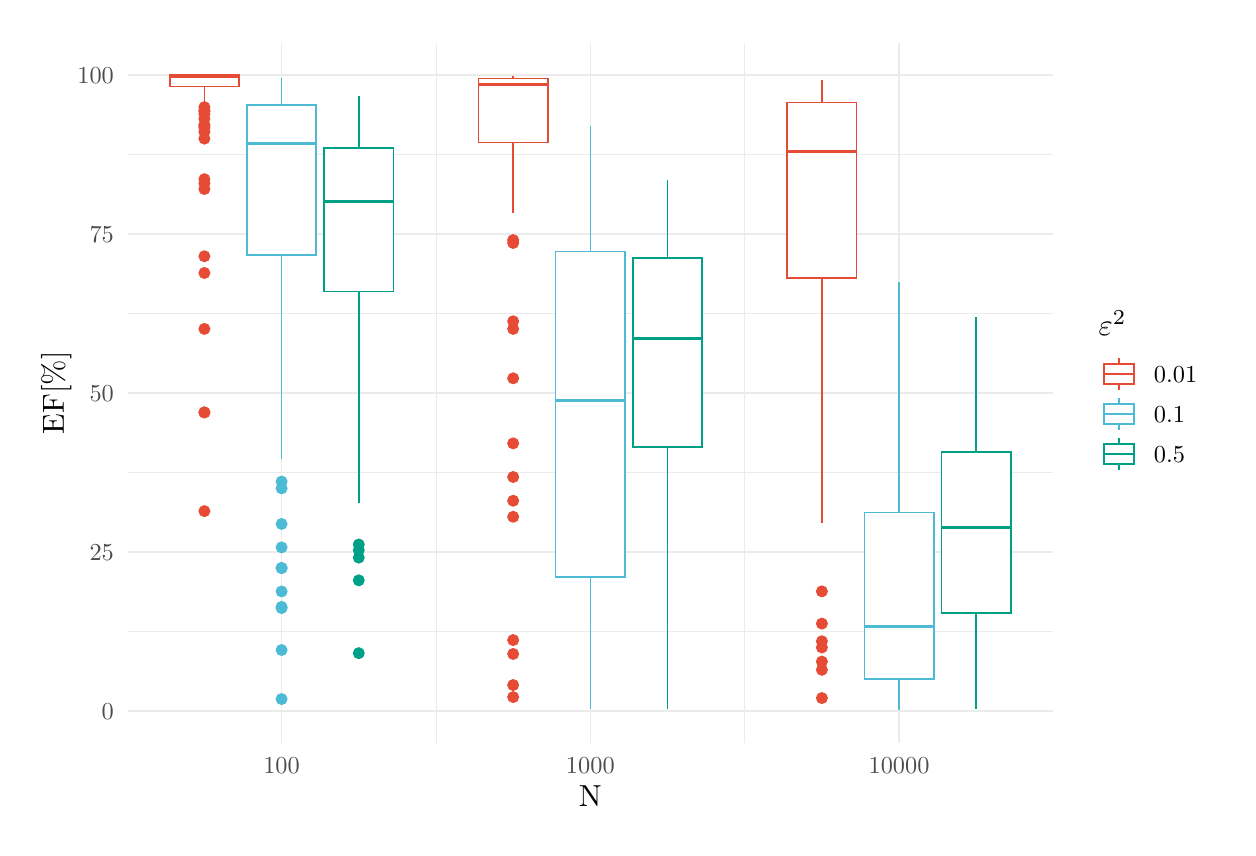
\begin{tikzpicture}[x=1pt,y=1pt]
\definecolor{fillColor}{RGB}{255,255,255}
\path[use as bounding box,fill=fillColor,fill opacity=0.00] (0,0) rectangle (433.62,289.08);
\begin{scope}
\path[clip] ( 36.11, 30.69) rectangle (370.53,283.58);
\definecolor{drawColor}{gray}{0.92}

\path[draw=drawColor,line width= 0.3pt,line join=round] ( 36.11, 70.92) --
	(370.53, 70.92);

\path[draw=drawColor,line width= 0.3pt,line join=round] ( 36.11,128.39) --
	(370.53,128.39);

\path[draw=drawColor,line width= 0.3pt,line join=round] ( 36.11,185.87) --
	(370.53,185.87);

\path[draw=drawColor,line width= 0.3pt,line join=round] ( 36.11,243.35) --
	(370.53,243.35);

\path[draw=drawColor,line width= 0.3pt,line join=round] (147.54, 30.69) --
	(147.54,283.58);

\path[draw=drawColor,line width= 0.3pt,line join=round] (259.10, 30.69) --
	(259.10,283.58);

\path[draw=drawColor,line width= 0.6pt,line join=round] ( 36.11, 42.18) --
	(370.53, 42.18);

\path[draw=drawColor,line width= 0.6pt,line join=round] ( 36.11, 99.66) --
	(370.53, 99.66);

\path[draw=drawColor,line width= 0.6pt,line join=round] ( 36.11,157.13) --
	(370.53,157.13);

\path[draw=drawColor,line width= 0.6pt,line join=round] ( 36.11,214.61) --
	(370.53,214.61);

\path[draw=drawColor,line width= 0.6pt,line join=round] ( 36.11,272.08) --
	(370.53,272.08);

\path[draw=drawColor,line width= 0.6pt,line join=round] ( 91.75, 30.69) --
	( 91.75,283.58);

\path[draw=drawColor,line width= 0.6pt,line join=round] (203.32, 30.69) --
	(203.32,283.58);

\path[draw=drawColor,line width= 0.6pt,line join=round] (314.88, 30.69) --
	(314.88,283.58);
\definecolor{drawColor}{RGB}{230,75,53}
\definecolor{fillColor}{RGB}{230,75,53}

\path[draw=drawColor,line width= 0.4pt,line join=round,line cap=round,fill=fillColor] ( 63.86,251.38) circle (  1.96);

\path[draw=drawColor,line width= 0.4pt,line join=round,line cap=round,fill=fillColor] ( 63.86,248.98) circle (  1.96);

\path[draw=drawColor,line width= 0.4pt,line join=round,line cap=round,fill=fillColor] ( 63.86,180.22) circle (  1.96);

\path[draw=drawColor,line width= 0.4pt,line join=round,line cap=round,fill=fillColor] ( 63.86,206.48) circle (  1.96);

\path[draw=drawColor,line width= 0.4pt,line join=round,line cap=round,fill=fillColor] ( 63.86,254.00) circle (  1.96);

\path[draw=drawColor,line width= 0.4pt,line join=round,line cap=round,fill=fillColor] ( 63.86,259.06) circle (  1.96);

\path[draw=drawColor,line width= 0.4pt,line join=round,line cap=round,fill=fillColor] ( 63.86,150.08) circle (  1.96);

\path[draw=drawColor,line width= 0.4pt,line join=round,line cap=round,fill=fillColor] ( 63.86,256.14) circle (  1.96);

\path[draw=drawColor,line width= 0.4pt,line join=round,line cap=round,fill=fillColor] ( 63.86,234.33) circle (  1.96);

\path[draw=drawColor,line width= 0.4pt,line join=round,line cap=round,fill=fillColor] ( 63.86,252.89) circle (  1.96);

\path[draw=drawColor,line width= 0.4pt,line join=round,line cap=round,fill=fillColor] ( 63.86,232.80) circle (  1.96);

\path[draw=drawColor,line width= 0.4pt,line join=round,line cap=round,fill=fillColor] ( 63.86,230.78) circle (  1.96);

\path[draw=drawColor,line width= 0.4pt,line join=round,line cap=round,fill=fillColor] ( 63.86,260.36) circle (  1.96);

\path[draw=drawColor,line width= 0.4pt,line join=round,line cap=round,fill=fillColor] ( 63.86,253.55) circle (  1.96);

\path[draw=drawColor,line width= 0.4pt,line join=round,line cap=round,fill=fillColor] ( 63.86,258.87) circle (  1.96);

\path[draw=drawColor,line width= 0.4pt,line join=round,line cap=round,fill=fillColor] ( 63.86,114.39) circle (  1.96);

\path[draw=drawColor,line width= 0.4pt,line join=round,line cap=round,fill=fillColor] ( 63.86,200.43) circle (  1.96);

\path[draw=drawColor,line width= 0.4pt,line join=round,line cap=round,fill=fillColor] ( 63.86,257.88) circle (  1.96);

\path[draw=drawColor,line width= 0.4pt,line join=round,line cap=round,fill=fillColor] ( 63.86,150.02) circle (  1.96);

\path[draw=drawColor,line width= 0.6pt,line join=round] ( 63.86,271.93) -- ( 63.86,272.07);

\path[draw=drawColor,line width= 0.6pt,line join=round] ( 63.86,267.84) -- ( 63.86,262.13);
\definecolor{fillColor}{RGB}{255,255,255}

\path[draw=drawColor,line width= 0.6pt,fill=fillColor] ( 51.31,271.93) --
	( 51.31,267.84) --
	( 76.41,267.84) --
	( 76.41,271.93) --
	( 51.31,271.93) --
	cycle;

\path[draw=drawColor,line width= 1.1pt] ( 51.31,271.62) -- ( 76.41,271.62);
\definecolor{drawColor}{RGB}{77,187,213}
\definecolor{fillColor}{RGB}{77,187,213}

\path[draw=drawColor,line width= 0.4pt,line join=round,line cap=round,fill=fillColor] ( 91.75,109.75) circle (  1.96);

\path[draw=drawColor,line width= 0.4pt,line join=round,line cap=round,fill=fillColor] ( 91.75, 79.34) circle (  1.96);

\path[draw=drawColor,line width= 0.4pt,line join=round,line cap=round,fill=fillColor] ( 91.75,101.28) circle (  1.96);

\path[draw=drawColor,line width= 0.4pt,line join=round,line cap=round,fill=fillColor] ( 91.75, 46.48) circle (  1.96);

\path[draw=drawColor,line width= 0.4pt,line join=round,line cap=round,fill=fillColor] ( 91.75, 64.19) circle (  1.96);

\path[draw=drawColor,line width= 0.4pt,line join=round,line cap=round,fill=fillColor] ( 91.75, 93.88) circle (  1.96);

\path[draw=drawColor,line width= 0.4pt,line join=round,line cap=round,fill=fillColor] ( 91.75, 93.76) circle (  1.96);

\path[draw=drawColor,line width= 0.4pt,line join=round,line cap=round,fill=fillColor] ( 91.75,122.61) circle (  1.96);

\path[draw=drawColor,line width= 0.4pt,line join=round,line cap=round,fill=fillColor] ( 91.75, 85.36) circle (  1.96);

\path[draw=drawColor,line width= 0.4pt,line join=round,line cap=round,fill=fillColor] ( 91.75, 79.78) circle (  1.96);

\path[draw=drawColor,line width= 0.4pt,line join=round,line cap=round,fill=fillColor] ( 91.75,125.06) circle (  1.96);

\path[draw=drawColor,line width= 0.6pt,line join=round] ( 91.75,261.10) -- ( 91.75,270.84);

\path[draw=drawColor,line width= 0.6pt,line join=round] ( 91.75,206.87) -- ( 91.75,133.20);
\definecolor{fillColor}{RGB}{255,255,255}

\path[draw=drawColor,line width= 0.6pt,fill=fillColor] ( 79.20,261.10) --
	( 79.20,206.87) --
	(104.30,206.87) --
	(104.30,261.10) --
	( 79.20,261.10) --
	cycle;

\path[draw=drawColor,line width= 1.1pt] ( 79.20,247.32) -- (104.30,247.32);
\definecolor{drawColor}{RGB}{0,160,135}
\definecolor{fillColor}{RGB}{0,160,135}

\path[draw=drawColor,line width= 0.4pt,line join=round,line cap=round,fill=fillColor] (119.64,102.33) circle (  1.96);

\path[draw=drawColor,line width= 0.4pt,line join=round,line cap=round,fill=fillColor] (119.64,100.27) circle (  1.96);

\path[draw=drawColor,line width= 0.4pt,line join=round,line cap=round,fill=fillColor] (119.64, 97.58) circle (  1.96);

\path[draw=drawColor,line width= 0.4pt,line join=round,line cap=round,fill=fillColor] (119.64, 89.37) circle (  1.96);

\path[draw=drawColor,line width= 0.4pt,line join=round,line cap=round,fill=fillColor] (119.64, 63.06) circle (  1.96);

\path[draw=drawColor,line width= 0.6pt,line join=round] (119.64,245.64) -- (119.64,264.45);

\path[draw=drawColor,line width= 0.6pt,line join=round] (119.64,193.75) -- (119.64,117.25);
\definecolor{fillColor}{RGB}{255,255,255}

\path[draw=drawColor,line width= 0.6pt,fill=fillColor] (107.09,245.64) --
	(107.09,193.75) --
	(132.20,193.75) --
	(132.20,245.64) --
	(107.09,245.64) --
	cycle;

\path[draw=drawColor,line width= 1.1pt] (107.09,226.34) -- (132.20,226.34);
\definecolor{drawColor}{RGB}{230,75,53}
\definecolor{fillColor}{RGB}{230,75,53}

\path[draw=drawColor,line width= 0.4pt,line join=round,line cap=round,fill=fillColor] (175.43,126.72) circle (  1.96);

\path[draw=drawColor,line width= 0.4pt,line join=round,line cap=round,fill=fillColor] (175.43, 62.77) circle (  1.96);

\path[draw=drawColor,line width= 0.4pt,line join=round,line cap=round,fill=fillColor] (175.43,211.28) circle (  1.96);

\path[draw=drawColor,line width= 0.4pt,line join=round,line cap=round,fill=fillColor] (175.43, 47.19) circle (  1.96);

\path[draw=drawColor,line width= 0.4pt,line join=round,line cap=round,fill=fillColor] (175.43,182.99) circle (  1.96);

\path[draw=drawColor,line width= 0.4pt,line join=round,line cap=round,fill=fillColor] (175.43,212.32) circle (  1.96);

\path[draw=drawColor,line width= 0.4pt,line join=round,line cap=round,fill=fillColor] (175.43, 51.54) circle (  1.96);

\path[draw=drawColor,line width= 0.4pt,line join=round,line cap=round,fill=fillColor] (175.43,138.87) circle (  1.96);

\path[draw=drawColor,line width= 0.4pt,line join=round,line cap=round,fill=fillColor] (175.43,180.21) circle (  1.96);

\path[draw=drawColor,line width= 0.4pt,line join=round,line cap=round,fill=fillColor] (175.43, 67.79) circle (  1.96);

\path[draw=drawColor,line width= 0.4pt,line join=round,line cap=round,fill=fillColor] (175.43,162.38) circle (  1.96);

\path[draw=drawColor,line width= 0.4pt,line join=round,line cap=round,fill=fillColor] (175.43,112.33) circle (  1.96);

\path[draw=drawColor,line width= 0.4pt,line join=round,line cap=round,fill=fillColor] (175.43,118.13) circle (  1.96);

\path[draw=drawColor,line width= 0.6pt,line join=round] (175.43,270.66) -- (175.43,271.72);

\path[draw=drawColor,line width= 0.6pt,line join=round] (175.43,247.63) -- (175.43,222.28);
\definecolor{fillColor}{RGB}{255,255,255}

\path[draw=drawColor,line width= 0.6pt,fill=fillColor] (162.88,270.66) --
	(162.88,247.63) --
	(187.98,247.63) --
	(187.98,270.66) --
	(162.88,270.66) --
	cycle;

\path[draw=drawColor,line width= 1.1pt] (162.88,268.45) -- (187.98,268.45);
\definecolor{drawColor}{RGB}{77,187,213}

\path[draw=drawColor,line width= 0.6pt,line join=round] (203.32,208.19) -- (203.32,253.54);

\path[draw=drawColor,line width= 0.6pt,line join=round] (203.32, 90.60) -- (203.32, 43.02);

\path[draw=drawColor,line width= 0.6pt,fill=fillColor] (190.77,208.19) --
	(190.77, 90.60) --
	(215.87, 90.60) --
	(215.87,208.19) --
	(190.77,208.19) --
	cycle;

\path[draw=drawColor,line width= 1.1pt] (190.77,154.31) -- (215.87,154.31);
\definecolor{drawColor}{RGB}{0,160,135}

\path[draw=drawColor,line width= 0.6pt,line join=round] (231.21,205.74) -- (231.21,233.88);

\path[draw=drawColor,line width= 0.6pt,line join=round] (231.21,137.67) -- (231.21, 42.94);

\path[draw=drawColor,line width= 0.6pt,fill=fillColor] (218.66,205.74) --
	(218.66,137.67) --
	(243.76,137.67) --
	(243.76,205.74) --
	(218.66,205.74) --
	cycle;

\path[draw=drawColor,line width= 1.1pt] (218.66,176.71) -- (243.76,176.71);
\definecolor{drawColor}{RGB}{230,75,53}
\definecolor{fillColor}{RGB}{230,75,53}

\path[draw=drawColor,line width= 0.4pt,line join=round,line cap=round,fill=fillColor] (286.99, 57.04) circle (  1.96);

\path[draw=drawColor,line width= 0.4pt,line join=round,line cap=round,fill=fillColor] (286.99, 65.12) circle (  1.96);

\path[draw=drawColor,line width= 0.4pt,line join=round,line cap=round,fill=fillColor] (286.99, 60.01) circle (  1.96);

\path[draw=drawColor,line width= 0.4pt,line join=round,line cap=round,fill=fillColor] (286.99, 85.39) circle (  1.96);

\path[draw=drawColor,line width= 0.4pt,line join=round,line cap=round,fill=fillColor] (286.99, 73.74) circle (  1.96);

\path[draw=drawColor,line width= 0.4pt,line join=round,line cap=round,fill=fillColor] (286.99, 46.83) circle (  1.96);

\path[draw=drawColor,line width= 0.4pt,line join=round,line cap=round,fill=fillColor] (286.99, 67.36) circle (  1.96);

\path[draw=drawColor,line width= 0.6pt,line join=round] (286.99,262.03) -- (286.99,270.08);

\path[draw=drawColor,line width= 0.6pt,line join=round] (286.99,198.53) -- (286.99,110.21);
\definecolor{fillColor}{RGB}{255,255,255}

\path[draw=drawColor,line width= 0.6pt,fill=fillColor] (274.44,262.03) --
	(274.44,198.53) --
	(299.54,198.53) --
	(299.54,262.03) --
	(274.44,262.03) --
	cycle;

\path[draw=drawColor,line width= 1.1pt] (274.44,244.33) -- (299.54,244.33);
\definecolor{drawColor}{RGB}{77,187,213}

\path[draw=drawColor,line width= 0.6pt,line join=round] (314.88,113.84) -- (314.88,197.09);

\path[draw=drawColor,line width= 0.6pt,line join=round] (314.88, 53.80) -- (314.88, 42.37);

\path[draw=drawColor,line width= 0.6pt,fill=fillColor] (302.33,113.84) --
	(302.33, 53.80) --
	(327.43, 53.80) --
	(327.43,113.84) --
	(302.33,113.84) --
	cycle;

\path[draw=drawColor,line width= 1.1pt] (302.33, 72.66) -- (327.43, 72.66);
\definecolor{drawColor}{RGB}{0,160,135}

\path[draw=drawColor,line width= 0.6pt,line join=round] (342.77,135.84) -- (342.77,184.37);

\path[draw=drawColor,line width= 0.6pt,line join=round] (342.77, 77.54) -- (342.77, 42.91);

\path[draw=drawColor,line width= 0.6pt,fill=fillColor] (330.22,135.84) --
	(330.22, 77.54) --
	(355.32, 77.54) --
	(355.32,135.84) --
	(330.22,135.84) --
	cycle;

\path[draw=drawColor,line width= 1.1pt] (330.22,108.44) -- (355.32,108.44);
\end{scope}
\begin{scope}
\path[clip] (  0.00,  0.00) rectangle (433.62,289.08);
\definecolor{drawColor}{gray}{0.30}

\node[text=drawColor,anchor=base east,inner sep=0pt, outer sep=0pt, scale=  0.88] at ( 31.16, 39.15) {0};

\node[text=drawColor,anchor=base east,inner sep=0pt, outer sep=0pt, scale=  0.88] at ( 31.16, 96.63) {25};

\node[text=drawColor,anchor=base east,inner sep=0pt, outer sep=0pt, scale=  0.88] at ( 31.16,154.10) {50};

\node[text=drawColor,anchor=base east,inner sep=0pt, outer sep=0pt, scale=  0.88] at ( 31.16,211.58) {75};

\node[text=drawColor,anchor=base east,inner sep=0pt, outer sep=0pt, scale=  0.88] at ( 31.16,269.05) {100};
\end{scope}
\begin{scope}
\path[clip] (  0.00,  0.00) rectangle (433.62,289.08);
\definecolor{drawColor}{gray}{0.30}

\node[text=drawColor,anchor=base,inner sep=0pt, outer sep=0pt, scale=  0.88] at ( 91.75, 19.68) {100};

\node[text=drawColor,anchor=base,inner sep=0pt, outer sep=0pt, scale=  0.88] at (203.32, 19.68) {1000};

\node[text=drawColor,anchor=base,inner sep=0pt, outer sep=0pt, scale=  0.88] at (314.88, 19.68) {10000};
\end{scope}
\begin{scope}
\path[clip] (  0.00,  0.00) rectangle (433.62,289.08);
\definecolor{drawColor}{RGB}{0,0,0}

\node[text=drawColor,anchor=base,inner sep=0pt, outer sep=0pt, scale=  1.10] at (203.32,  7.64) {N};
\end{scope}
\begin{scope}
\path[clip] (  0.00,  0.00) rectangle (433.62,289.08);
\definecolor{drawColor}{RGB}{0,0,0}

\node[text=drawColor,rotate= 90.00,anchor=base,inner sep=0pt, outer sep=0pt, scale=  1.10] at ( 13.08,157.13) {EF[\%]};
\end{scope}
\begin{scope}
\path[clip] (  0.00,  0.00) rectangle (433.62,289.08);
\definecolor{drawColor}{RGB}{0,0,0}

\node[text=drawColor,anchor=base west,inner sep=0pt, outer sep=0pt, scale=  1.10] at (387.03,177.78) {$\varepsilon^2$};
\end{scope}
\begin{scope}
\path[clip] (  0.00,  0.00) rectangle (433.62,289.08);
\definecolor{drawColor}{RGB}{230,75,53}

\path[draw=drawColor,line width= 0.6pt] (394.25,158.20) --
	(394.25,160.37);

\path[draw=drawColor,line width= 0.6pt] (394.25,167.59) --
	(394.25,169.76);
\definecolor{fillColor}{RGB}{255,255,255}

\path[draw=drawColor,line width= 0.6pt,fill=fillColor] (388.83,160.37) rectangle (399.67,167.59);

\path[draw=drawColor,line width= 0.6pt] (388.83,163.98) --
	(399.67,163.98);
\end{scope}
\begin{scope}
\path[clip] (  0.00,  0.00) rectangle (433.62,289.08);
\definecolor{drawColor}{RGB}{77,187,213}

\path[draw=drawColor,line width= 0.6pt] (394.25,143.74) --
	(394.25,145.91);

\path[draw=drawColor,line width= 0.6pt] (394.25,153.14) --
	(394.25,155.31);
\definecolor{fillColor}{RGB}{255,255,255}

\path[draw=drawColor,line width= 0.6pt,fill=fillColor] (388.83,145.91) rectangle (399.67,153.14);

\path[draw=drawColor,line width= 0.6pt] (388.83,149.53) --
	(399.67,149.53);
\end{scope}
\begin{scope}
\path[clip] (  0.00,  0.00) rectangle (433.62,289.08);
\definecolor{drawColor}{RGB}{0,160,135}

\path[draw=drawColor,line width= 0.6pt] (394.25,129.29) --
	(394.25,131.46);

\path[draw=drawColor,line width= 0.6pt] (394.25,138.69) --
	(394.25,140.85);
\definecolor{fillColor}{RGB}{255,255,255}

\path[draw=drawColor,line width= 0.6pt,fill=fillColor] (388.83,131.46) rectangle (399.67,138.69);

\path[draw=drawColor,line width= 0.6pt] (388.83,135.07) --
	(399.67,135.07);
\end{scope}
\begin{scope}
\path[clip] (  0.00,  0.00) rectangle (433.62,289.08);
\definecolor{drawColor}{RGB}{0,0,0}

\node[text=drawColor,anchor=base west,inner sep=0pt, outer sep=0pt, scale=  0.88] at (406.98,160.95) {0.01};
\end{scope}
\begin{scope}
\path[clip] (  0.00,  0.00) rectangle (433.62,289.08);
\definecolor{drawColor}{RGB}{0,0,0}

\node[text=drawColor,anchor=base west,inner sep=0pt, outer sep=0pt, scale=  0.88] at (406.98,146.50) {0.1};
\end{scope}
\begin{scope}
\path[clip] (  0.00,  0.00) rectangle (433.62,289.08);
\definecolor{drawColor}{RGB}{0,0,0}

\node[text=drawColor,anchor=base west,inner sep=0pt, outer sep=0pt, scale=  0.88] at (406.98,132.04) {0.5};
\end{scope}
\end{tikzpicture}
%
        }
        \caption{Empirical \acrshort{ef} for the setup of \Cref{ex:ess_failure} for varying sample sizes $N$ and $\varepsilon^{2}$ and $M=100$ replications. Here $\G = \mathcal N(0,1)$ and $\P = \frac{1}{2} \left( \mathcal N (0,1) + \mathcal N(0, \varepsilon^{-2}) \right)$. In all scenarios the second moment $\rho$ is infinite, thus high \acrshortpl{ef} are misleading us to believe that importance sampling performs well when it does not.}
        \label{fig:ess_failure}
    \end{figure}

\end{example}

As an alternative, we may want to assess whether importance sampling has converged through the empirical variance of $\hat \zeta_{N}$,\footnote{As the following arguments depend on the sample size $N$, we mark this dependency by adding $N$ to the subscript of the estimator.} i.e., 
$$
\widehat\var \left( \hat\zeta_{N} \right) = \frac{1}{N}\left(\frac{1}{N} \sum_{i = 1}^N w_{i}^{2} f(X^{i})^{2} - \hat \zeta_{N}^{2}\right)
$$
is, while seemingly natural, flawed \citep{Chatterjee2018Sample}.
Indeed, the authors show that for any given threshold $\epsilon$ we may find an $N$ which only depends on $\epsilon$, such that the probability that the empirical variance exceeds $\epsilon$ for this $N$ is small. This is summarized in the following theorem.

\begin{theorem}[{\cite[Theorem 2.1]{Chatterjee2018Sample}}]
    \label{thm:variance_failure}
    Given any $\epsilon > 0$, there exists $N \leq \epsilon^{-2} 2^{1 + \epsilon^{-3}}$ such that the following is true. Take any $\G$ and $\P$ as in \Cref{thm:chatterje2018Thm1}, and any $f: \mathcal X \to \R$ such that $ \lVert f \rVert_{L^{2}(\P)} \leq 1.$ Then 
    $$
        \mathbb P \left( \widehat \var \left( \hat \zeta_{N} \right) < \epsilon\right) \geq 1 - 4 \epsilon.
    $$
\end{theorem}

The problem here is that $N$ does not depend on $\G$ and $\P$, so we may choose $\G$ almost singular to $\P$. As an example, take $\P = \mathcal N(0, 1)$ and $\G = \mathcal N(0, \sigma^{2})$ for $\sigma^{2} > \frac{1}{2}$. The weights are then given by $$w(x) = \sigma \exp \left( - \frac{x^{2}}{2} \left( 1 - \frac{1}{\sigma^{2}} \right) \right),$$
and for $X \sim \G$ the variance of $w(X)X$ is 
\begin{align}
    \label{eq:variance-wxx}
\tau^{2} = \var \left( w(X)X \right) = \frac{\sigma^{4}}{\left( 2 \sigma^{2} - 1 \right)^{\frac{3}{2}}}
\end{align}
which goes to $\infty$ as $\sigma^2$ does, see the appendix for details. Thus, for a pre-specified $\epsilon > 0$, let $N$ be as in \Cref{thm:variance_failure} and choose $\sigma^{2}$ such that $\var \left( \hat\zeta_{N} \right) = \frac {\tau^{2}}N$ is larger than, say, $10\epsilon$. By the preceding theorem, we would, with large probability, observe a small empirical variance and thus declare $\hat\zeta_{N}$ to have converged, whereas, in reality, we would need a sample size that is $100$ times as large.

Thus using the empirical variance as a threshold for convergence should be avoided, at least for importance sampling where the weights can be evaluated exactly. For self-normalized importance sampling, the authors do not provide such a theorem. As a remedy \citep{Chatterjee2018Sample} suggest the heuristic $q_{N} = \mathbb E Q_{N}$ where
$$
Q_{N} = \max_{1\leq i\leq N} W_{i} \in [0, 1].
$$
This judges whether importance sampling has collapsed to just a few particles and is itself amenable to Monte-Carlo integration, by repeatedly sampling $N$ samples from $\G$ and calculating the weights. 
As this requires multiple runs of importance sampling, it may, however, be prohibitively expensive in practice.

In the following sections, we will predominantly take the position that we are interested in finding a good particle approximation $\hat\P_{N}$ of the form \Cref{eq:is-particle-approximation} over finding the optimal proposal $\G^{\ast}$ from \Cref{prop:minimum_MSE_IS} and assume that the importance sampling weights can only be evaluated up to a constant. 
This has several reasons: First of all, for most problems considered in this thesis $\P$ is usually a conditional distribution, e.g. $\P = \mathbb P^{X|Y=y}$ for states $X$ and observations $Y$ in the \acrshort{ssm} context. Should the appropriate densities exist, evaluating the weights amounts to calculating 
$$
\rnd{\mathbb P^{X| Y= y}}{\G}(x) = \frac{p(x|y)}{g(x)} = \frac{p(y|x)p(x)}{g(x)p(y)} \propto \frac{p(y|x)p(x)}{g(x)}.
$$
In these situations $p(y) = \int p(x,y)\d x$ is usually intractable. For $\G^{\ast}$ we are in the same situation, where the evaluation of the integration constant $\P \lvert f \rvert$ is infeasible, but the density $\lvert f(x)\rvert p(x)$ is available.
% do not focus on a single f
Second, focusing on the particle approximation allows us to consider multiple test functions $f$, e.g. focus on different marginals of $\P$, which is usually what practitioners are interested in. 
%Third, for maximum likelihood estimation (\Cref{sec:maximum_likelihood_estimation}), we will see that these two notions coincide.
% simplify notation: P always target, G always proposal
Finally, this allows us to simplify the notation used in this thesis. $\P$ will always be the probability measure of interest and $\G$ the proposal. In later parts of this thesis, we will predominantly perform Gaussian importance sampling, i.e. $\G = \mathcal N(\mu, \Sigma)$, hence a handy mnemonic is to think of $\G$ as a \textbf{G}aussian proposal.

Let us now turn towards the problem of finding a good proposal $\G$ for a given $\P$. 

\subsection{\texorpdfstring{\Acrfull{la}}{Laplace approximation}}
\label{subsec:la}

The \acrfull{la} goes back to Laplace \citep{Laplace1986Memoir} who invented the technique to approximate moments of otherwise intractable distributions. Since \citep{Tierney1986Accurate,Tierney1989Fully} rediscovered its use to approximate posterior means and variances, it has been a staple method for approximate inference.
The method is based on a second-order Taylor series expansion of the log target density $\log p(x)$ around its mode $\hat x$, i.e. matching mode and curvature. Assuming the density is sufficiently smooth, we have
\begin{align}
    \label{eq:LA_approximation}
\log p(x) \approx \log p(\hat x) + \underbrace{\nabla_{x} \log p (\hat x)}_{= 0} \left( x - \hat x \right) + \frac{1}{2} (x - \hat x)^{T} H (x - \hat x)
\end{align}
where $H$ is the Hessian of $\log p$ evaluated at $\hat x$. As $\log p (\hat x)$ does not depend on $x$, the right-hand side can be seen (up to additive constants) as the density of a Gaussian distribution with mean $\hat x$ and covariance matrix $\Sigma = - H^{-1}$. Thus using $\G = \mathcal N (\hat x, -H^{-1})$ as a proposal in importance sampling seems promising. 
% degenerate case when $H$ is not PSD
If $\hat x$ is the unique global mode of $p$ and $H$ is negative definite, the \gls{la} yields an actual Gaussian distribution. 
% numerics
To obtain the \acrshort{la} in practice, a Newton-Raphson scheme may be used, which conveniently tracks $H$ as well. Furthermore, if $\P$ includes more structure, e.g. it is the smoothing density in the \acrshort{ssm} context, we may be able to exploit this structure to design efficient Newton-Raphson schemes, see \Cref{subsec:glssm-approach}.

% advantages / disadvantages
The main advantage of the \gls{la} is that it is usually fast to obtain and, for sufficiently well-behaved distributions on a moderate dimensional space, provides reasonably high \gls{ess}. Additionally, the Newton-Raphson iterations to find the mode and Hessian are robust and require no simulation, unlike the other methods discussed further below.
For the \glspl{ssm} we consider in this thesis, the numerical methods can be implemented using the Kalman filter and smoother \citep{Shephard1997Likelihood,Durbin1997Monte}, even in the degenerate case where $H$ is indefinite \citep{Jungbacker2007Monte}, see also \Cref{subsec:glssm-approach}.

However, as the \gls{la} is a local approximation, it may be an inappropriate description of the global behavior of the target, see \Cref{ex:la_failure} for a breakdown of \gls{la}, and the simulation studies presented in \Cref{sec:simulation_studies}. 
Additionally, even if the \gls{la} works in principle, its \gls{ess} will usually degenerate quickly once the dimension increases whereas the \gls{cem} and \gls{eis} do so at a slower pace.

%\glsreset{vm}
\subsection{\texorpdfstring{\Acrfull{vmm}}{Variance Minimization method}}
As we have discussed above, the second moment 
$$
\rho = \G [w^{2}]
$$
plays an important role in the performance of importance sampling. Naturally, we may want to choose $\G$ such that $\rho$ becomes minimal. To this end we consider tractable, parametric proposals $\left( \G_{\psi} \right)_{\psi \in \Psi}$ for a parameter set $\Psi$, where usually $\Psi \subseteq \R^{k}$. Noticing that $\G_{\psi} w_{\psi} = 1$, we see that minimizing $\rho_{\psi} = \G_{\psi}[w^{2}_\psi]$ over $\Psi$ is equivalent to minimizing
$$
\var \left( w_{\psi}(X_{\psi}) \right) = \G_{\psi}[w_{\psi}^2] - \G_{\psi}[w_{\psi}]^{2} = \rho_{\psi} - 1,
$$
over $\Psi$ where $X_{\psi} \sim \G_{\psi}$. This is the \gls{vmm} 
\glsreset{cem}
\subsection{The \texorpdfstring{\Acrfull{cem}}{Cross-Entropy method}}
\label{subsec:cem}
Recall from our discussion surrounding \Cref{thm:chatterje2018Thm1} that for importance sampling to be effective, we should have a small \acrshort{kld} between the target $\P$ and the proposal $\G$. As the \acrshort{kld} depends on global properties, i.e. the Radon-Nikodym derivative $\rnd{\P}{\G}$, minimizing it should lead to a global approximation of $\P$, improving on the local-approximation provided by the \acrshort{la}.

The \gls{cem}\citep{Rubinstein1999CrossEntropy,Rubinstein2004CrossEntropy} implements this idea and selects from a parametric family $ \left( \G_{\psi} \right)_{\psi \in \Psi}$ of proposals the one that minimizes the \gls{kld} to the target. Here $\Psi$ is usually a subset of $\R^{k}$. We will usually assume the existence of a common dominating measure $\mu$ for both $\P$ and all $\G_{\psi}$, $\psi \in \Psi$ with corresponding densities $p$ and $g_{\psi}$, $\psi \in \Psi$. The importance sampling weights are then given by 
$$
w_{\psi}(x) = \frac{p(x)}{g_{\psi}(x)},
$$
$x \in \mathcal X$, or, if either on of $p$ and $g_\psi$ is only available up to a constant, by 
$$
\tilde w_{\psi} (x) \propto \frac{p(x)}{g_{\psi}(x)}.
$$
If the dependence on $\psi$ is not of interest or the particular $\psi$ is obvious from the context, we may drop the subscript. 

The \acrshort{cem} finds $\psi_{\text{CE}}$ which solves the following optimization problem
\begin{align*}
    \psi_{\text{CE}} &= \argmin_{\psi \in \Psi} \Dkl{\P}{\G_{\psi}} \\
    &= \argmin_{\psi \in \Psi} \P \left[ \log w_{\psi}\right]
\end{align*}
The existence and uniqueness of $\psi_{\text{CE}}$ will depend heavily on the choice of parametric family $(\G_{\psi})_{\psi \in \Psi}$ and $\P$. 

If $\P$ and $\G_{\psi}$ possess densities $p$ and $g_{\psi}$ w.r.t. some common measure $\mu$, the same for all $\psi$, we may reformulate the optimization problem to maximize the cross-entropy between $p$ and $g_{\psi}$ instead:
\begin{align}
    \begin{split}
    \psi_{\text{CE}} &= \argmin_{\psi \in \Psi} \P \left[\log p \right] - \P \left[\log g_{\psi}\right] \\
    &= \argmax_{\psi \in \Psi} \P \left[\log g_{\psi}\right]
    \end{split} \label{eq:ce_argmax}.
\end{align}
Suppose now that $\psi \mapsto \log g_{\psi}(x)$ is (strictly) concave for $\P$-almost every $x \in \mathcal X$ and $\Psi$ is a convex subset of $\R^{k}$. Then $\psi \mapsto \P \left[\log g_{\psi}\right]$ is (strictly) concave as well. As a consequence, we may apply the usual results from convex optimization, i.e. every local maximum is a global one, the set of maximizers is convex and if $\psi \mapsto \log g_{\psi}(x)$ is strictly convex for $\P$-almost every $x$, there is at most one maximizer \todo{ref}.

As we have seen in \Cref{lem:log-concavity}, the densities of exponential families are log-concave in the natural parameter, and as such they will be the ideal candidates for our investigations. 

%\begin{theorem}[consistencty of $\hat\psi_{\text{CE}}$]
%    \label{thm:ce-m-estimator}
%    Assume the following technical conditions apply:
%    \begin{itemize}
%        \item[A1] Uniform consistency of importance sampling
%            $$\sup_{\psi \in \Psi}\lVert \hat \G_N (w\log g_\psi) - \G(w \log g_\psi) \rVert \stackrel{P}{\to} 0$$ 
%        \item[A2] Regularity condition
%            $$ \partial_\psi \P \left(\log g_\theta\right) = \P \left(\partial_\theta \log g_\theta\right) $$
%            for all $\psi \in \Psi$
%        \item[A3] positive definite misspecified Fisher information
%            $$ \P \left(\left(\partial_\psi \log g_\theta\right)\left(\partial_\theta \log g_\theta\right)^T\right) > 0$$
%    \end{itemize}
%
%    Then $\hat\psi_{\text{CE}}$ is a consistent estimator of $\psi_{\text{CE}}$.
%\end{theorem}
%
%\begin{theorem}[asymptotic normality of $\hat\psi_{\text{CE}}$]
%    
%\end{theorem}

% analytical solution, MLE
An additional attractive property of the \gls{cem} for exponential families with natural parameter $\psi \in \R^{k}$, the optimal $\psi_{\text{CE}}$ only depends on the expected value $\P [T]$. 

\begin{proposition}[The \acrshort{cem} for exponential families]
    \label{prop:cem_exponential_families}
    Let $\left( \G_{\psi} \right)_{\psi \in \Psi}$ form a $k$-dimensional natural exponential family with log-densities 
    $$
    \log g_{\psi}(x) = \log h(x) + \psi^{T} T(x) - \log Z(\psi),
    $$
    and convex parameter space $\Psi \subseteq \R^{k}$. 
    Suppose $T, \log (h) \in L^{1}(\P)$.

    If there is a $\psi$ such that 
    $$
    \P[T] = \G_{\psi} [T],
    $$
    then $\psi = \pce$ is a maximizer of \Cref{eq:ce_argmax}. If $\cov_{\G_{\psi}} T$ is positive definite for all $\psi\in\Psi$, then the maximizer is unique.
\end{proposition}

\begin{proof}
    The target may be rewritten as
    $$
    \psi \mapsto f(\psi) = \P \left[\log g_{\psi}(x)\right]= \P [\log h] - \log Z(\psi) + \psi^{T} \P [T].
    $$
    As $\log Z(\psi)$ is the cumulant-generating function of $\G_{\psi}$ it is twice differentiable, and so is $f$. The gradient of $\log Z(\psi)$ is 
    $$
    \nabla_{\psi} \log Z(\psi) = \G_{\psi} T
    $$
    and its Hessian is 
    $$
    H_{\psi} \log Z(\psi) = \cov_{\G_{\psi}} T
    $$
    the covariance of $T$ under $\G_{\psi}$. Thus the Hessian of $f$ is 
    $$
    H_{\psi} f = - \cov_{\G_{\psi}} T,
    $$
    which is negative-semi-definite. Thus $f$ is concave, and any local maximizer $\psi$ is a global maximizer. The gradient of $f$ is 
    $$
        \nabla_{\psi} f(\psi) = \P[T] - \G_{\psi} [T],
    $$
    thus the optimal $\psi_{\text{CE}}$ solves
    $$
    \P[T] = \G_{\pce}[T].
    $$
    If $\cov_{\G_{\psi}} T$ is positive definite for all $\psi \in \Psi$, $f$ is strictly concave, and the maximizer is unique.
\end{proof}
As a consequence, the \acrshort{cem} for natural exponential families reduces to matching the moments of the sufficient statistic of the target and proposal.
In many cases, this system of equations can be solved analytically or by gradient descent algorithms.
Let us discuss the assumptions and applicability of this proposition. Assuming that $T, \log h \in L^{1}(\P)$ is necessary for the target to be finite, so it cannot be dropped. The proof of uniqueness relies on $\cov_{\G_{\psi}} T$ being positive definite, to ensure that $\psi \mapsto \log Z(\psi)$ is strictly convex. This could also be achieved by requiring the exponential family to be minimal, see \citep[Theorem 1.13 (iv)]{Brown1986Fundamentals}. The existence of a $\psi$ such that $\P T = \G_{\psi} T$ is not restrictive for most commonly used distributions: for the (multivariate) normal, Poisson, negative binomial and binomial distribution there is always a unique solution, as the sufficient statistics consist of means and covariances. 

While $\P T$ is usually not available, it is itself amenable to importance sampling. Given a proposal $\G$ we may estimate $\P T$ by $\hat\P_N T = \sum_{i = 1}^{N} W^{i} T(X^{i})$ for $X^{1}, \dots, X^{N} \iid \G$ and auto-normalized importance sampling weights $W^{i}$ and in turn, applying \Cref{prop:cem_exponential_families}, estimate $\psi_{\text{CE}}$ by $\hat \psi_{\text{CE}}$ solving
$$
\hat \P_N T = \G_{\hpce} T.
$$
As $T, \log h \in L^{1}(\hat \P_{N})$, the only conditions we have to check to apply the above proposition is that this equation has a unique solution and that $\Psi$ is convex. 

In what follows, we will derive novel results on the performance of this estimator. In particular, we will investigate under which conditions $\hpce$ is consistent and asymptotically normal. While we restrict ourselves here to the setting of $k$-dimensional natural exponential families, these results should generalize to other classes of distributions as well. The advantage that this class of families has is that due to the structure of the densities, they provide straightforward (regularity) conditions for the asymptotic results to hold.

% proof: appeal to vdV, pd ensures that M(\theta) is convex, so global maximum unique and well separated
$\hat\psi_{\text{CE}}$ is a Z-estimator, i.e. an estimator that arises from solving a random system of equations, and we can analyze its asymptotic behavior using standard results from the theory of Z-estimators. 
The following theorem of \citep{VanderVaart2000Asymptotic} will be useful in analyzing the asymptotic behavior of the estimators we consider in this thesis. We state it here, using our notation, for completeness.

\begin{theorem}[asymptotic normality of Z-estimators, {\citep[Theorem 5.21]{VanderVaart2000Asymptotic}}]
    \label{thm:clt_z_est_vdv}
    For every $\psi$ in an open subset of $\R^{k}$, let $x \mapsto f_{\psi}(x)$ be a measurable vector-valued function such that, for every $\psi_{1}$ and $\psi_{2}$ in a neighborhood of $\psi_{0}$ and a measurable function $\dot f$ with $\G \left[\dot f\right] < \infty$,
    \begin{align}
    \label{eq:clt-vdv-local-lipschitz}
    \lVert f_{\psi_{1}}(x) - f_{\psi_{2}}(x)\rVert \leq \dot f(x) \lVert \psi_{1} - \psi_{2}\rVert \tag{LL}.
    \end{align}

    Assume that $\G \left[\lVert f_{\psi_{0}}\rVert \right] < \infty$ and that the map $\psi \mapsto \G \left[f_{\psi}\right]$ is differentiable at $\psi_{0}$, with nonsingular derivative matrix $B^{-1}$. Let $X_{1}, \dots, X_{N} \iid \G$ and $\hat \G_{N} = \sum_{i = 1}^{N} \delta_{X^{i}}$. If $\hat\psi_{N}$ fulfills $$\hat\G_{N} \left[f_{\hat\psi_{N}}\right] = o_{P} \left( N^{-\frac{1}{2}} \right),$$ and $\hat\psi_{N} \to \psi_{0}$ in probability, then
    \begin{align}
        \label{eq:clt-vdv}
        \sqrt{N} \left( \hat\psi_{N} - \psi_{0} \right) \Dto \mathcal N(0, BMB^{T}),
    \end{align}
    where $M = \G f_{\psi_{0}} f_{\psi_{0}}^{T}$.
\end{theorem}

\begin{notation}[central limit theorem for Z-estimators]
    \label{not:notation-clt}
    The central limit theorems derived in this and the next section will make frequent use of \Cref{thm:clt_z_est_vdv}. We will use the following consistent notation in the statement of theorems and their proofs:
    \begin{itemize}
        \item $f_\psi(x): \R^{k} \to \R^{k}$ the estimating equation              
        \item $B = \left(\G\partial_{\psi} f_{\psi}\right)^{-1}$ the bread matrix
        \item $M = \G f_{\psi}f_{\psi}^{T}$ the meat matrix
        \item $V = BMB$ the asymptotic covariance matrix
        \item $\log g_{\psi}(x) = \psi^{T}T(x) + \log h(x) - \log Z(\psi)$ the density of the natural exponential family considered
        \item $\dot z (\psi) = \nabla_{\psi}\log Z(\psi) = \G_{\psi} T$ the derivative of the log-normalizing constant $\psi \mapsto \log Z(\psi)$
        \item $\ddot z(\psi) = \partial_{\psi} \dot z(\psi) =\cov_{\G_{\psi}}T$ the Hessian of the log-normalizing constant $\psi \mapsto \log Z(\psi)$
    \end{itemize}
    The naming of $B$ and $M$ stems from the sandwich estimator \citep{White1982Maximum}, where the bread $B$ is the Jacobian of the estimating equations $\P f_{\psi} = 0$ and the meat $M$ is the covariance matrix of $f_{\psi}$ under $\P$, thus making a \glqq{}meat sandwich\grqq{}.
\end{notation}

\todo{discussion on relevance and novelty of these results}
\begin{theorem}[consistency of $\hat \psi_{\text{CE}}$]
    \label{thm:ce-consistent}
    \todo{from van der Vaart/Casella Berger}
\end{theorem}


\begin{theorem}[asymptotic normality of $\hat \psi_{\text{CE}}$]
    \label{thm:ce-clt}
    %\todo{require unique solution?}
    Let $\G_{\psi}$ form a natural exponential family with densities $g_{\psi}(x) = \frac{h(x)}{Z(\psi)} \exp \left( \psi^{T}T(x)\right) $ w.r.t. $\mu$. Let $\G, \P$ be two other probability measures such that $\G \ll \P$ and let $W = \frac{\d \P}{\d \G}$ be the normalized importance sampling weights. 
    Suppose further that 
    \begin{enumerate}[label={\bfseries(A{\arabic*})}]
        \item\label{it:exist-unique-psice} $\G_{\hpce} T = \hat\P_{N} T$ $\mu$-a.s. has a unique solution $\hpce$,
        \item\label{it:zdot-ll} $\psi \mapsto \nabla_\psi \log Z(\psi)$ is locally Lipschitz around $\psi_{\text{CE}}$,
        \item\label{it:w-t-wt-L2} $W,T$ and $WT$ possess finite second moments  w.r.t. $\G$,
        \item\label{it:FI-psd} the Fisher information $I(\psi_{\text{CE}})$ is positive definite and equal to $-\ddot z(\pce)$, additionally $\psi \mapsto I(\psi)$ is continuous, and
        \item\label{it:ce-regularity} the regularity conditions of \Cref{thm:ce-consistent} hold.
    \end{enumerate}

    Then, as $N$ goes to $\infty$,
    $$
        \sqrt{N} \left(\hat\psi_\text{CE} - \psi_{\text{CE}}\right) \Dto \mathcal N \left(0, V_{\text{CE}}\right)
    $$
    where 
    $$
    V_{\text{CE}} = B_\ce M_\ce B_\ce,%I(\psi_{\text{CE}})^{-1}  \text{Cov}_{\G} \left( W (T - \G_{\pce}T) \right) I(\psi_{\text{CE}})^{-1},
    $$
    with 
    \begin{align*}
        B_{\ce} &= I(\pce)^{-1}, \\
        M_{\ce} &= \cov_{\G} \left( W (T - \G_{\pce}T) \right).
    \end{align*}
    Moreover $\G (W(T - \G_{\pce}T))) = 0$, so we may estimate $V_{\text{CE}}$ consistently by plug-in:
    $$
    \hat V_{\text{CE}} = I(\hat\psi_{\text{CE}})^{-1}  \left(\sum_{i = 1}^N W^{2}_{i} \left(T(X^{i}) - \G_{\hpce}T \right)\left(T(X^{i}) - \G_{\hpce} T\right)^{T} \right)I(\hat\psi_{\text{CE}})^{-1}.
    $$
\end{theorem}

\begin{proof} We check that the conditions of the central limit theorem for Z-estimators (\Cref{thm:clt_z_est_vdv}) are fulfilled. This proof uses the notation established in \Cref{not:notation-clt}. Consider the estimating equations for $\pce$ 
    $$x\mapsto f_\psi(x) = \nabla_{\psi} \left(w(x)\log g_{\psi}(x)\right) = w(x) T(x) - w(x) \dot z (\psi),$$ where $w(x)$ are the unnormalized importance sampling weights. 
    By \ref{it:exist-unique-psice} $\hat \P_{N} f_{\hpce} = 0$ $\mu$-a.s., so it remains to show that $\hpce \to \pce$  in probability, which is implied by \Cref{thm:ce-consistent}.
    
    As $$\left\lVert f_{\psi_1}(x) - f_{\psi_2}(x)\right\rVert = w(x) \left\lVert \dot z (\psi_1) - \dot z(\psi_2)\right\rVert$$ for all $\psi_{1}, \psi_{2}\in \Psi$,  $\G w < \infty $ and \ref{it:zdot-ll} imply the local Lipschitz condition \Cref{eq:clt-vdv-local-lipschitz} in \Cref{thm:clt_z_est_vdv}.
    Furthermore, by \ref{it:w-t-wt-L2} it holds
    %\todo{fix: no triangle equation (squared norm)}
    $$
    \G \left\lVert f_\psi \right\rVert^2 \leq \G w^2 \left\lVert \dot z(\psi) \right\rVert ^2  + 2 \lVert \dot z(\psi) \rVert \G \lVert wT\rVert + \G \left\lVert wT\right\rVert^2 < \infty.
    $$

    Additionally $\psi \mapsto\G f_\psi = (\G w) \dot z (\psi) + \G wT$ is differentiable everywhere, with Jacobian $(\G w) \ddot z(\psi)$, where  $\ddot z(\psi) = \partial_\psi \dot z(\psi)$ is the Hessian of the cumulant generating function, which equals the negative Fisher information $-I(\pce)$ as $\G_{\psi}, \psi \in \Psi$ form a natural exponential family and the regularity conditions \ref{it:ce-regularity} allow differentiation under the integral.
    Thus we see that 
    $$
    \G f_{\pce} = \P \left( \dot z(\pce) + T \right) = \dot z (\pce) + \P T = 0,
    $$
    by definition of $\pce$, so $$\text{Cov}_{\G} \left( w(T - \nabla_{\pce} \log Z (\pce)) \right) = \text{Cov}_{\G}(f_{\pce}) = \G f_{\pce}f_{\pce}^{T}.$$
    As $W = \frac{w}{\G w}$
    By \Cref{eq:clt-vdv} the asymptotic covariance matrix is 
    $$
    V_{\ce} = B_{\ce}M_{\ce}B_{\ce}
    $$
    which shows the asymptotic normality. 

    Estimating $B_{\ce}$ by $\hat B_{\ce}= I(\hpce)$ and $$M_{\ce} = \G W^{2} (T - \G_{\pce}T)(T - \G_{\pce}T)^{T} = \P W (T - \G_{\pce})(T - \G_{\pce})^T$$ by $$\hat M_{\ce} = \hat\P_{N} W \left( T - \G_{\hpce} T \right)\left( T - \G_{\hpce} T \right)^{T}$$
    yields the stated plug-in estimator. 
    The promised consistency follows from \ref{it:w-t-wt-L2} and \ref{it:FI-psd}.
\end{proof}

The form of the asymptotic covariance matrix is that of the sandwich estimator \citep{White1982Maximum}, corrected for the importance sampling with $\G$. This is not surprising: the \acrshort{cem} essentially performs maximum likelihood estimation of $\psi$ where the data come from the misspecified $\P$. Additionally, we have to correct the variance for performing importance sampling with $\G$, instead of sampling directly from $\P$.

As mentioned above, if $(\G_\psi)_{\psi \in \Psi}$ do not form an exponential family, $\hat\psi_{\text{CE}}$ will still be consistent and asymptotically normal, provided the usual regularity conditions for M-estimators, or Z-estimators if $\log g_{\psi}$ is sufficiently smooth, apply. 

% break-down in higher dimensions?

% iterative procedure, CRNs

% applications of CEM
The \gls{cem} is routinely used for estimating failure probabilities for rare events \citep{Homem-de-Mello2007Study} and has been applied to Bayesian inference \citep{Engel2023Bayesian,Ehre2023Certified} and optimal control problems \citep{Kappen2016Adaptive,Zhang2014Applications}.
\todo{more lit. review CEM}

\glsreset{eis}
\subsection{\texorpdfstring{\Acrfull{eis}}{Efficient importance sampling}}
\label{subsec:eis}
\gls{eis} \citep{Richard2007Efficient} provides an alternative to the \gls{cem}. Instead of minimizing the \gls{kld} between the target $\P$ and proposal $\G_{\psi}, \psi \in \Psi$, \gls{eis} aims at minimizing the variance of the logarithm of importance sampling weights. 
Our discussion of \citep{Chatterjee2018Sample}, \Cref{thm:chatterje2018Thm1}, especially \Cref{lem:bounded-log-variance}, suggests that this is worthwhile. 
Thus, \acrshort{eis} finds $\peis$ which is a feasible solution to the following optimization problem
\begin{align}
    \label{eq:eis_optim}
\min_{\psi \in \Psi} \text{Var}_{\P} \left[ \log w_{\psi} \right] = \min_{\psi \in \Psi} \P \left[ \log w_{\psi} - \P \log w_{\psi} \right]^{2},
\end{align}
where, as in the last section, $\log w_{\psi} = \log p - \log g_{\psi}$.

Two problems arise: $\P [\log w_{\psi}] = \Dkl{\P}{\G_{\psi}}$ is usually intractable and we usually only have access to the unnormalized weights $\frac{\tilde w_{\psi}}{\G_{\psi} \left[ w_{\psi} \right]} = w_{\psi}$, with unknown integration constant $\G_{\psi} \left[ w_{\psi} \right]$. Both can be dealt with by introducing the nuisance parameter $\lambda = \P \left[ \log \tilde w_{\psi} \right]$, utilizing the fact that the mean is the minimizer of the squared distance functional with the minimum value equal to the variance, should it exist. Indeed 
$$
    \log w_{\psi} - \P [\log w_{\psi}] = \log \tilde w_{\psi} - \log \G_{\psi} [\tilde w_{\psi}] - \P \left[ \log \tilde w_{\psi} \right] + \log \G_{\psi}[\tilde w_{\psi}] = \log \tilde w_{\psi} - \P \left[ \log \tilde w_{\psi} \right],
$$
so
$$
    \min_{\psi \in \Psi} \P \left[ \log w_{\psi} - \P \left[ \log w_{\psi} \right] \right]^{2} = \min_{\psi \in \Psi, \lambda \in \R} \P \left[ \log \tilde w_{\psi} - \lambda \right]^{2},
$$
where $\psi\in \Psi$ is a minimizer of the left-hand side if, and only if, $(\psi, \lambda) \in \Psi \times \R$ with $\lambda = \P \left[ \log \tilde w_{\psi} \right]$ is a minimizer of the right-hand side. 

Similar to the \gls{cem} we restrict our in-depth analysis to natural exponential family proposals where $$\log g_{\psi}(x) = \psi^{T}T(x) - \log Z(\psi).$$ In this case the optimization problem is reduced to
\begin{align}
    \label{eq:eis_exponential_families}
    \min_{\psi \in \Psi, \lambda \in \R} \P \left[ \log p - \psi^{T}T - \lambda \right]^{2},
\end{align}
a weighted linear least squares problem. As we consider unnormalized weights $\tilde w$, we are additionally able to get rid of the potentially non-linear term $\log Z(\psi)$.
Noticing that this is a convex objective function in $\psi$ which, similar to the \acrshort{cem}, will be very useful to derive asymptotics later on. For now, we begin with studying the existence and uniqueness of $\peis$ similar to \Cref{prop:cem_exponential_families}.

\begin{lemma}[\acrshort{eis} for exponential families]
    \label{prop:eis_exponential_families}
    Let $\left( \G_{\psi} \right)_{\psi \in \Psi}$ form a k-dimensional natural exponential family with log-densities 
    $$
        \log g_{\psi}(x) = \psi^{T} T(x) - \log Z(\psi)
    $$
    for $\Psi \subseteq \R^{k}$. Suppose that $\log p, T \in L^{2}(\P)$. 

    If there is a $\peis \in \Psi$ with
    \begin{align}
        \label{eq:peis-analytical}
        \cov_{\P} \left( T \right)\peis = \cov_{\P} \left(T, \log p \right)
    \end{align}
    it is a global minimizer of \Cref{eq:eis_optim}. If $\cov_{\P} \left( T \right)$ is non-singular,
    $$
    \peis = \cov_{\P} (T) ^{-1} \cov _{\P} (T, \log p )
    $$
    is the unique global minimizer.
\end{lemma}

\begin{proof}
    Under the proposed conditions, we may consider \Cref{eq:eis_exponential_families} instead, where the moment conditions on $\log p $ and $T$ ensure that the problem is well-posed, i.e. the target is finite for all $\psi \in \Psi$. 
    Thus the optimal $ \left( \peis, \lambda_{\eis} \right)$ are given by the \gls{blup} of $\log p $ by the sufficient statistic $T$ under $\P$ for $\peis$ and $\P \left[ \log \tilde w_{\peis} \right]$ for $\lambda_{\eis}$. Standard results from multivariate regression theory imply that the \acrshort{blup} is given by any solution of
    $$
        \cov_{\P} (T) \peis = \cov_{\P} (T, \log p),
    $$
    i.e. $\peis$ as stated in the lemma. Furthermore, if $\cov_{\P} (T)$ is non-singular, the solution to this equation is unique.
    
\end{proof}

As the optimal $\peis$ depends on several unknown quantities, \gls{eis} proceeds like the \gls{cem} and employs importance sampling with a proposal $\G$, estimating $\peis$ by
$$
\left(\hat \lambda,\hat \psi_{\text{EIS}}\right) = \argmin_{\lambda,\psi} \hat\P_{N} \left[ \log \tilde w_{\psi} - \lambda \right]
$$
where $X^{1}, \dots, X^{N} \iid \G$. 
Again, if $\G_{\psi}, \psi \in \Psi$ form an exponential family with natural parameter $\psi$, this optimization problem turns into a weighted least squares problem, so we can estimate $\peis$ with the standard weighted least squares estimator
$$
\left( \hat\lambda', \hpeis \right) = \left(\mathbf X^{T}\mathbf W\mathbf X\right)^{-1}\mathbf X^{T}\mathbf W y%
$$
where the random design matrix $\mathbf X$\footnote{if $\mathbf X\mathbf W \mathbf X$ is not invertible, replace the inverse by the Moore-Penrose pseudoinverse} and diagonal weights matrix $\mathbf W$ are given by
\begin{align*}
\mathbf X &= \begin{pmatrix}
    1 & T(X^{1})^{T} \\
    \dots&\dots\\
    1 & T(X^{N})^{T} \\
\end{pmatrix}\\
\intertext{and}
\mathbf W &= \text{diag} \left( W^{1}, \dots, W^{N} \right),
\end{align*}
and the observations are 
\begin{align*}
y = \left( \log p(X^{1}), \dots, \log p(X^{N}) \right)^{T} \in \R^{N}.
\end{align*}

Alternatively, replacing $\P$ by $\hat\P_{N}$ in \Cref{eq:peis-analytical}, we obtain the equivalent formulation
\begin{align}
    \label{eq:hpeis-cov}
    \hpeis = \cov_{\hat\P_{N}} (T)^{-1} \cov_{\hat \P_{N}} \left( T, \log p \right),
\end{align}
as long as $\cov_{\hat \P_{N}} T$ is non-singular.

An attractive feature of \gls{eis} is that if the target $\P$ is a member of the exponential family of proposals, i.e. there is a $\psi_{\P}\in\Psi$ such that $\P = \G_{\psi_{\P}}$, then \gls{eis} finds the optimal $\peis = \psi_{\P}$ a.s. for a finite number of samples.

\begin{proposition}[Finite sample convergence of \gls{eis}]
    \label{prop:eis-finite-sample}
    Suppose $\G_{\psi}, \psi \in \Psi \subseteq \R^{k}$ for a natural exponential family w.r.t. Lebesgue measure, where the support of the sufficient statistic $\operatorname{supp} T$ is open in $\R^{k}$. 
    Furthermore let $\G$ be a probability measure on $\R^{m}$ that is equivalent to $\P$, i.e. $\G \ll \P$ and $\P \ll \G$. 

    If there is a $\psi_{\P} \in \Psi$ such that $\P = \G_{\psi_{\P}}$, then $\hpeis = \psi_{\P}$ a.s. for $N \geq k$. 
\end{proposition}

\begin{proof}
   As $\P$ stems from the same exponential family as $\G_{\psi}$, the pseudo-observations are $$\log p  = \psi_{\P}^T T - \log Z(\psi_{\P}).$$ Thus $\cov_{\hat \P_{N}} \left( T, \log p  \right) = \cov_{\hat \P_{N}} \left( T \right)\psi_{\P}$. 
   If we can show that $\cov_{\hat\P_{N}} T$ is non-singular, \Cref{eq:hpeis-cov} implies that $\hpeis = \psi_{\P}$ a.s.. 

   If $\cov_{\hat \P_{N}} T$ were singular, there would exist a $\psi \in \R^{k}$ such that
   $$
   \psi^{T} \cov_{\hat\P_{N}} (T) \psi = \cov_{\hat \P_{N}} \left( \psi^{T}T \right) = 0.
   $$
    In this case the a.s. non-zero $W^{i}(X^{i}) T(X^{i})$ would lie in the orthogonal complement $\psi^{\perp}$ for all $i = 1, \dots, N$. As the weights are a.s. positive by the assumed equivalence of $\G$ and $\P$, the same holds true for $T(X^{i}), i = 1,\dots, N$.
   If $N$ is bigger than $k$, the probability that this happens is $0$, as $\operatorname{supp} T $ is open. Thus $\cov_{\hat \P_{N}} T$ is non-singular almost surely and the result is shown.
\end{proof}

Note that if in the above proposition only $\G_{\psi} \gg \P$ holds, we obtain, by a similar argument, that $$\mathbb P \left( \hpeis = \psi_{\P} \right) \stackrel{N\to\infty}\longrightarrow 1.$$
Additionally, we then have to take care of the event $ \{ w(X) = 0 \}$, whose probability is now potentially positive.

We now turn to deriving asymptotics for $\hpeis$. As for the \acrshort{cem}, we start with proving that $\hpeis$ consistently estimates $\peis$.
For this we need to ensure that $\peis$ is the unique solution to \Cref{eq:eis_optim}, as otherwise, consistent estimators of $\peis$ cannot exist. 
As \Cref{eq:eis_exponential_families} is a linear least squares problem, the objective function is convex, and so we can apply \Cref{thm:haberman-consistent} and \Cref{prop:is-consistency}.

\begin{theorem}[consistency of $\hpeis$]
    \label{thm:eis-consistent}
    Let $\left( \G_{\psi} \right)_{\psi \in \Psi}$ form a $k$-dimensional natural exponential family with log-densities 
    $$
        \log g_{\psi}(x) = \psi^{T}T(x) - \log Z(\psi)
    $$
    for convex $\Psi \subseteq \R^{k}$. Let $\G \gg \P$ be a proposal and suppose that 
    \begin{enumerate}
        \item $\log p, T \in L^{2}(\P)$ and
        \item $\cov_\P (T)$ is non-singular,
        \item $\peis \in \operatorname{int} \Psi.$ 
    \end{enumerate}
    
    Then 
    $$
        \hpeis \stackrel{N \to \infty}\longrightarrow \peis
    $$
    almost surely.
\end{theorem}

\begin{proof}
    We follow the same strategy as in the proof of \Cref{thm:cem-consistent}. Let 
    \begin{align*}
        b: \R^{p} \times \R^{k + 1} \to [-\infty, \infty)  && b(x,\psi') = \begin{cases}
            -\frac{1}{2} \left( \log p(x) - \psi^{T}T(x) - \lambda \right)^{2} & \psi \in \Psi \\
            -\infty &  \text{ else,}
        \end{cases}
    \end{align*}
    where $\psi' = (\psi, \lambda) \in \R^{k + 1}$. For fixed $x$ this function is concave, as its Hessian is negative semi-definite:
    $$
        H_{\psi'} b(x, \psi') = -\begin{pmatrix}
            1 & T(x)^{T} \\
            T(x) & T(x)T(x)^{T}
        \end{pmatrix} = -\begin{pmatrix} 1 & T(x)^{T} \end{pmatrix} \begin{pmatrix} 1 & T(x)^{T} \end{pmatrix}^{T},
    $$
    if $\psi \in \Psi$. Let $X^{1}, \dots, X^{N} \iid \P$ and let $\tilde \P _{N}$ be their empirical distribution. For $\psi \in \Psi, \lambda \in \R$ we have 
    $$
        \P \left[ b(\cdot, \psi') \right] = - \frac{1}{2} \P \left[ \left( \log p - \psi^{T}T - \lambda\right)^{2} \right] < \infty,
    $$
    as $\log p, T\in L^{2}(\P)$. Let us now check that conditions \ref{it:C1} - \ref{it:C3} are fulfilled. 

    \ref{it:C1} is fulfilled, as we assumed $\peis \in \operatorname{int} \Psi$. \ref{it:C2} holds, as $\peis$ is the unique global maximizer by \Cref{prop:eis_exponential_families}, as $\cov (T)$ is non-singular.
    \ref{it:C3} obviously holds. 

    Thus $\hpeis$ is strongly consistent if $\G = \P$. If $\G$ is different from $\P$, we can apply \Cref{prop:is-consistency}, where the existence of M-estimators is ensured by \Cref{eq:hpeis-cov}, using the Moore-Penrose inverse if $\cov_{\hat\P_{N}}(T)$ is singular. 
\end{proof}

As \Cref{eq:hpeis-cov} expresses $\hpeis$ in terms of empirical covariances, we could alternatively prove consistency by ensuring that the empirical covariances are consistent as well, for which we would need to ensure that fourth-order moments of $\log p$ and $T$ w.r.t. $\P$ exist. This strategy may be fruitful if $\peis$ does not lie in the interior of $\Psi$, although the more sophisticated treatment of \citep{Haberman1989Concavity} may also be applicable under these circumstances.

Additionally, if fourth-order moments exist, we can derive a central limit theorem, similar to \Cref{thm:cem-clt}, for \acrshort{eis}.

% region CLT proof
\begin{theorem}[\acrshort{clt} for $\hpeis$]
    \label{thm:eis-clt}
    Let $\left( \G_{\psi} \right)_{\psi \in \Psi}$ form a $k$-dimensional natural exponential family with log-densities 
    $$
    \log g_{\psi}(x) = \psi^{T} T(x) - \log Z(\psi),
    $$
    and convex parameter space $\Psi \subseteq \R^{k}$. Let $\G \gg \P$ be a proposal with weights $w = \rnd{\P}{\G}$. 

    Assume that
    \begin{enumerate}
        \item\label{it:secondISmomentsexist}$w T_{i}T_{j}, w (\log p)^{2} \in L^{2}(\G)$ for $i,j = 1, \dots, k$,
        \item\label{it:fourthmomentsexist} $\log p, T_i \in L^{4}(\P)$ for all $i = 1, \dots, k$
        \item $\cov_{\P}(T)$ is non-singular and $\peis \in \operatorname{int} \Psi$.
    \end{enumerate}

    Then 
    $$
        \sqrt{N} (\hpeis - \peis) \convD \Normal (0, BMB)
    $$
    where $B = \cov_{\P}(T)^{-1}$ and 
    $$
    M = \cov_{\G} \left( w \left( \log p - \peis^{T}T - \lambda_{\eis} - \P[T] \right)T \right).
    $$
\end{theorem}

\begin{proof}
    Similar to the proof of \Cref{thm:cem-clt}, we combine \Cref{thm:haberman-clt} and \Cref{prop:is-clt}. Let 
    \begin{align*}
        b : \mathcal X \times \R^{k + 1} \to [-\infty, \infty) && b(x, \psi') =  \begin{cases}
            -\frac{1}{2} \left( \log p(x) - \psi^{\prime T}T'(x) \right) & x \in \Psi \\
            -\infty & \text{else,}
        \end{cases}
    \end{align*}
    where $\psi' = (\psi, \lambda) \in \Psi \times\R$ and $T'(x) = \begin{pmatrix} T(x) & 1 \end{pmatrix}$. For $\psi \in \Psi$ the map $(\psi, \lambda) \to \P [b(\cdot, (\psi, \lambda))]$ is differentiable with gradient 
    $$
        \nabla_{\psi'} \P [b(\cdot, \psi')] = - \P \left[\left( \log p - \psi^{\prime T}T' \right) T'\right] = \begin{pmatrix}
            - \P \left[ T'\log p - T'T^{\prime T}\psi' \right] \\
            -\P \left[ \log p - \psi'^{T}T' \right]
        \end{pmatrix}
    $$
    and Hessian 
    $$
        H_{\psi'} \P[b(\cdot, \psi')] = -\P\left[T'T^{\prime T}\right] = - \begin{pmatrix}
            \P \left[ TT^{T} \right] & \P [T^{T}] \\
            \P [T] & 1
        \end{pmatrix}.
    $$
    The Hessian is negative definite, as for all $\psi\in \R^{k}, \lambda \in \R$ we have
    \begin{align*}
        \begin{pmatrix} \psi^{T} & \lambda \end{pmatrix} H_{\psi'} \P \left[ b(\cdot, \psi') \right]\begin{pmatrix} \psi^{T} & \lambda \end{pmatrix}^{T} &= - \left( \psi^{T} \cov_{\P} (T) \psi + \psi^{T}\P[T]\P[T]^{T}\psi + 2 \psi^{T}\P[T] \lambda + \lambda^{2}\right) \\
                                 &= - \left( \psi^{T}\cov_{\P}(T)\psi + (\lambda + \psi^{T}\P[T])^{2} \right) \leq 0,
    \end{align*}
    with equality if, and only if, both $\lambda$ and $\psi$ are $0$, as $\cov_{\P}(T)$ is assumed to be positive definite. Thus condition \ref{it:C7} is fulfilled.

    For condition \ref{it:C10}, we can verify that for all $i,j = 1,\dots, k+ 1$ 
    $$
        (\nabla_{\psi'} b(\cdot, \psi'))_{i}(\nabla_{\psi'} b(\cdot, \psi'))_{j} = \left( \log p - \psi^{\prime T}T' \right)^{2} T'_{i}T'_{j}
    $$
    is in $L^{1}(\P)$ by assumption \ref{it:fourthmomentsexist} and the Hölder inequality. 

    To apply \Cref{prop:is-clt} we need to show that $w(\cdot)b'(\cdot, \psi',\xi') \in L^{2}(\G)$ for all $\xi'\in\R^{k + 1}$ and all $\psi'$ in a neighborhood of $\peis$, for this it suffices that we show 
    $$
        w^{2}(\nabla_{\psi'} b(\cdot, \psi'))_{i}(\nabla_{\psi'} b(\cdot, \psi'))_{j} = w^{2}\left( \log p - \psi^{\prime T}T' \right)^{2} T'_{i}T'_{j}
    $$
    is in $L^{1}(\G)$, which holds, again, by assumption \Cref{it:secondISmomentsexist} and the Hölder inequality.

    We have thus shown a central limit theorem for $\hat\psi'_{\eis} = \left( \hpeis, \hat\lambda_{\eis} \right)$, i.e. 
    $$
        \sqrt{N} \left( \hat\psi'_{\eis} - \peis \right) \to \mathcal N(0, M'B'M')
    $$
    with $B' = - \left(H_{\psi'_{\eis}} \P \left[ b(\cdot, \psi'_{\eis}) \right]\right)^{-1}$ and $M' = \cov \left( w(X) \nabla_{\psi'_{\eis}} b(X,\psi'_{\eis}) \right)$ for $X \sim \G$. By using the inversion formula for block matrices, we obtain 
    \begin{align*}
        B' &= \begin{pmatrix}
            \P \left[ TT^{T} \right] & \P [T^{T}] \\
            \P [T] & 1
        \end{pmatrix}^{-1} = \begin{pmatrix}
            \Sigma + \mu\mu^{T} & \mu^{T} \\
            \mu & 1
        \end{pmatrix}^{-1} \\
        &= \begin{pmatrix}
            (\Sigma + \mu\mu^{T} - \mu\mu^{T})^{-1} & 0 \\
            0 & 1 - \mu^{T} (\Sigma + \mu\mu^{T})^{-1}\mu
        \end{pmatrix} \begin{pmatrix}
            I_{k} & - \mu^{T} \\
            -\mu(\Sigma + \mu\mu^{T})^{-1}& 1
        \end{pmatrix} \\
        &= \begin{pmatrix}
            \Sigma^{-1} & - \mu^{T}\Sigma^{-1}\\
            -\Sigma^{-1}\mu& 1 - \mu^{T} \left( \Sigma + \mu\mu^{T} \right)^{-1}\mu
        \end{pmatrix}
    \end{align*}
    where $\Sigma = \cov_{\P} (T)$ and $\mu = \P [T]$. Similarly, 
    $$
        M' = \begin{pmatrix}
            \cov_{\G} \left( w W_{\peis}T \right) &\cov_{\G} \left( w W_{\peis}T, w W_{\peis} \right) \\
            \cov_{\G} \left( w W_{\peis}, w W_{\peis}T \right) & \cov_{\G} \left( w W_{\peis} \right) 
        \end{pmatrix},
    $$
    where $W_{\peis} = \log p - \psi^{\prime T}_{\eis}T'$.

    If $\mu \neq 0$, we may change the sufficient statistic of the exponential family such that this holds, i.e. let $\tilde T = T - \P [T]$, then 
    $$
        \log g_{\psi}(x) = \psi^{T}T(x) - \log Z(\psi) = \psi^{T}\tilde T(x) - \log \tilde Z(\psi)
    $$
    where $\tilde Z(\psi) = \log Z(\psi) + \P [T]$. As $\peis$, \Cref{eq:peis-analytical}, only depends on $T - \P[T]$ under $\P$, this does not change $\peis$. Similarly, $\hpeis$, \Cref{eq:hpeis-cov}, is unaffected by subtracting a constant from $T$. Only 
    $$
        \tilde \lambda_{\eis} = \lambda_{\eis} + \P[T]
    $$
    and similarly $\hat\lambda_{\eis}$ are changed.
    
    Thus, without loss of generality, we may assume that $\P[T] = 0$. 
    Then 
    $$
        B' = \begin{pmatrix}
            \Sigma^{-1} & 0 \\
            0 & 1
        \end{pmatrix}
    $$
    is a diagonal matrix. Taking the $\peis$ marginal of the asymptotic normal distribution, we arrive at 
    $$
        \sqrt{N} \left( \hpeis - \peis \right) \to \mathcal N \left( 0, BMB \right)
    $$
    with $B = \cov_{\P}(T)$ and $M = \cov_{G} \left( w \left( \log p - \peis^{T}T - \lambda_{\eis} - \P[T] \right)T \right)$, as promised.
    
\end{proof}
% endregion 


A discussion of the assumptions of \Cref{thm:eis-consistent,thm:eis-clt} is in order. We start with the consistency result \Cref{thm:eis-consistent}. The integrability condition, i.e that $\log p, T \in L^{2}(\P)$ is necessary to ensure existence of $\peis$ and the existence of $\cov_{\P}(T)$ as well as $\peis \in \operatorname{int} \Psi$ ensure uniqueness, see also \Cref{prop:eis_exponential_families}. 

Regarding the central limit theorem \Cref{thm:eis-clt}, requiring the existence of higher order moments is natural. Unfortunately, there is no direct interpretation of these requirements as generalizations of the existence of $\rho$, as was the case for the \acrshort{cem}. 

The only integrability conditions related to the proposal $\G$ are those for $wT_{i}T_{j}$ and $w \log(p)^{2}$. 
Choosing $\left(\G_{\psi}\right)_{\psi \in \Psi}$ to consist of Gaussian distributions, the conditions on $T$ translate to the existence of certain polynomial moments of $w^{2}$ w.r.t. the proposal $\G$ (or $w$ w.r.t. $\P$). This technical condition, is not easily interpreted, as assuming existence of moments of the target distribution seem more natural than those involving the extra weighting term $w = \frac{p}{g}$, which depends on the proposal $\G$ as well. 
\section{Interim discussion}
\label{sec:interim-discussion}

Before we apply \gls{eis} and the \gls{cem} in the \gls{ssm} context, let us consolidate what we have achieved by the asymptotic analysis in the preceding two subsections and reason which of the two methods should be used in which circumstances.

% region optimal values
%% CE depends only on first moment of T, EIS also on second moments, as well as log p
We start with a discussion of the optimal values $\pce$ and $\peis$.
Notice that $\peis$ depends on second-order moments of the sufficient statistic $T$, as well as the shape of $\log p$, whereas the optimal parameter for the \gls{cem} $\pce$ depends only on the first-order moments of $T$. 
%% dependence on higher moments might help w/ better fit to heavier tail distributions
This dependence on higher-order moments may be beneficial for the \gls{eis} method, for example, if the covariance of $T$ under $\P$ is very different from that under $\G_{\psi}$. 
%% reiterate Dkl vs. log var

% endregion

% region assumptions
%% EIS requires higher moments to work, so might fail if target does not have these moments
The two methods differ concerning the assumptions that are required for uniqueness, consistency and the central limit theorem to hold if the proposals come from an exponential family. 
%% uniqueness
For uniqueness, \Cref{prop:cem_exponential_families} and \Cref{prop:eis_exponential_families}, both methods require that the covariance of $T$ is non-singular, however, the measures under which the covariance is considered differ: for the \gls{cem} we need $\cov_{\G_{\pce}} (T)$ to be non-singular, while for \gls{eis} the same has to hold for $\cov_{\P} (T)$. While the former is easy to ensure, the latter depends on the intractable target $\P$ and may be more difficult to verify in practice, depending on $T$. 

%% consistency & CLT
Regarding the consistency results, \Cref{thm:cem-consistent,thm:eis-consistent} as well as the central limit theorems, \Cref{thm:cem-clt,thm:eis-clt}, \gls{eis} requires that the sufficient statistic be twice as often $\P$-integrable as the \gls{cem}. Additionally, the \gls{eis} results assume that $\log p$ is sufficiently often $\P$-integrable. Therefore, \gls{eis} is, at first glance, more restrictive than the \gls{cem}. However, our application will perform importance sampling with Gaussian proposals where $T(x) = \begin{pmatrix} x \\ xx^{T}\end{pmatrix}$. For importance sampling to be consistent in this setting, we have to assume that the target has lighter tails than the Gaussian proposal, which implies that all polynomial moments of the target, and thus of $T$ exist. A similar argument can be made for $\log p$, and so the assumptions are likely to be fulfilled when Gaussian importance sampling is consistent.

% region asymptotic covariances
%% assuming Cov_P T approx Cov_psi T, main differences lies in Ms
To compare the asymptotic covariance matrices of both methods, note that both covariance matrices have the same ``{}bread-meat-bread''{} factorization, as they are asymptotic covariance matrices of M-estimators. We see that both $$B_{\ce} = I(\psi) = \cov_{\G_{\pce}}(T)^{-1}$$ and $$B_{\eis} = \cov_{\P}(T)^{-1}$$ are precision matrices of the sufficient statistic $T$, one with respect to the optimal \gls{cem} proposal and one with respect to the target. Thus, if $\P$ is well approximated by $\G_{\pce}$, we would expect these two components to be close to one another. 
For $$M_{\ce} = \cov_{\G} \left( w (T - \P[T]) \right)$$ and $$M_{\eis} = \cov_{\G}\left( w \log (w_{\peis})(T-\P[T]) \right),$$ there is a more notable difference, i.e. the presence of the $\log w_{\peis}$ term. If the \gls{eis} approximation performs well, we can expect this term to be small, as it is the prediction error of the least squares approximation of $\log g_{\psi}$ to $\log p$. Therefore, we expect that \gls{eis} outperforms the \gls{cem} in terms of asymptotic variance in these settings. In agreement with \Cref{prop:eis-finite-sample}, $M_{\eis} = 0$ if $\log p = \log g_{\psi_{\P}}$ so that $\peis = \psi_{\P}$.
%% however Mce might allow for optimization, by choosing G s.t. Cov wT is small, ie VM?
% endregion

% region choice of \G
Additionally, both $M_{\ce}$ and $M_{\eis}$ depend on the proposal $\G$, and indicate how one might tailor the initial proposal $\G$ to produce low-variance estimates. For the \gls{cem} we might choose $\G$ such that the trace or determinant of $\G [w^{2} (T - \P[T]) (T - \P [T])^{T}]$ becomes small. This is not necessarily achieved by the \gls{cem} proposal $\G_{\hpce}$, and so it may be worthwhile to investigate using two types of proposals in the \gls{cem}, one that makes $M_{\ce}$ small and $\G_{\pce}$. This is especially relevant as our simulation studies, \Cref{sec:simulation_studies}, suggest that the asymptotic covariance of the \gls{cem} is usually larger than that of \gls{eis}. For \gls{eis}, a similar approach might be fruitful, but is not as urgent as that for the \gls{cem}, as the asymptotic covariance of \gls{eis} is usually small enough to be feasible in practice.
% endregion

% region novelty / extension / outlook
%% asymptotic properties of both methods have not been studied to authors knowledge
Finally, let us stress that these asymptotic considerations are, to the author's knowledge, novel results and should be straightforward to extend if the proposals $\left(\G_{\psi}\right)_{\psi \in \Psi}$ do not form a natural exponential family. As any minimal exponential family may be reduced to a natural exponential family by reparametrization, see \citep[Theorem 1.9]{Brown1986Fundamentals}, the delta method can be used to derive \glspl{clt} in this case as well, as \Cref{prop:cem_exponential_families} and \Cref{prop:eis_exponential_families} still apply. If the family is not minimal the optimal values $\peis$ and $\pce$ may be non-unique, so we cannot hope to estimate them consistently. In this case the user should choose a minimal parametrization, see again \citep[Theorem 1.9]{Brown1986Fundamentals}. 
For non-exponential family proposals our results should also carry over, provided the usual regularity conditions ensuring uniqueness, consistency and asymptotic normality for M-estimators hold. If the objective functions are not concave as they are in our setting, one usually requires uniformly bounded third-order derivatives of the objective function to exist. 

Furthermore, our results can also be extended to the so-called \gls{vmm} which determines an optimal proposal by solving the following optimization problem:
$$
\psi_{\text{VM}} = \argmin_{\psi\in\Psi} \var_{\G_{\psi}} \left( w_{\psi}  \right) = \argmin_{\psi \in \Psi} \G_{\psi} \left[w_{\psi}^2\right] = \argmin_{\psi\in\Psi} \P \left[w_{\psi} \right],
$$
where the first equality holds as $\G_{\psi}[w_{\psi}] = 1$ for all $\psi$. Thus the \gls{vmm} chooses $\psi$ such that the second moment of importance sampling weights, $\rho$, becomes small. Again, this is sensible by the discussion surrounding $\rho$ and the \gls{ess}. Similar to the \gls{cem} and \gls{eis}, one uses importance sampling with a proposal $\G$ to approximate $\P [w_{\psi}]$ by $\hat\P_{N} [w_{\psi}]$, and solves this noisy version of the problem.
Unfortunately, there is no closed form for the optimal $\psi_{\text{VM}}$ or $\hat\psi_{\text{VM}}$, even if the proposals form a natural exponential family. Still, as $\psi \mapsto w_{\psi}(x)$ is convex, so is $\psi \mapsto \P [w_{\psi}]$, and we can apply \Cref{thm:haberman-consistent,thm:haberman-clt} in combination with \Cref{prop:is-consistency,prop:is-clt} to show, under suitable regularity conditions, the consistency and asymptotic normality of the method. 
% endregion

% region transition
Now that we have gained theoretical insight into optimal importance sampling, let us apply these insights to the \glspl{ssm} that we are interested in.
% endregion
\section{Gaussian importance sampling for state space models}
\label{sec:gaussian_importance_sampling_for_state_space_models}

% two types of proposals: direct, SSMs
For the types of models considered in this thesis, importance sampling is used to infer the posterior distribution. Given a state space model of the form \eqref{def:ssm} and observations $Y = Y_{:n}$, let $\P$ be the distribution of the states $X=X_{:n}$, conditional on $Y$ and $f$ be a function of interest. The task at hand is now to find a suitable proposal $\G$, using the methods presented in the last section. If $n$ is large, the posterior distribution lives in a high dimensional state of dimension $m\cdot n$, so to obtain $\G$ efficiently, we should exploit the available structure. Additionally, we want $\G$ to be tractable, so simulating from it is possible and evaluating the weights $w$ up to a constant is possible. 

The multivariate Gaussian distribution is a good candidate in this setting, as simulating from it is straightforward and its density can be evaluated analytically. However, naively performing the optimal importance sampling methods from the previous section for all multivariate Gaussians is computationally inefficient as the family of distributions has $\mathcal O((n\cdot m)^{2})$ many parameters. We can, however, exploit the available structure of the \gls{ssm} to find parameterizations with fewer parameters by either using smoothing distributions of \glspl{glssm} (\Cref{subsec:glssm-approach}) or approximating with a Gaussian discrete-time Markov process (\Cref{subsec:markov-approach}). 

% discuss if there actually is a Gaussian close to the target, see heavy tails etc.
Using Gaussian proposals, while computationally efficient, also comes with some drawbacks. The whole procedure hinges on the assumption that there is a Gaussian that is close to the target distribution. In the setting of \acrshortpl{ssm} this is not guaranteed, as the targets may contain multiple modes or heavy tails, features that may, in the worst case, lead to inconsistent importance sampling estimates. %At least for the models considered in \Cref{cha:analysis_of_selected_models}, the targets arise as posterior distributions of \gls{lcssm} and as such they are unimodal and have non-heavy tails, i.e. there is a Gaussian distribution such that importance sampling is feasible \todo{rethink, is this really the case, for LCSSM it depends on log-partition function of observations}. 
Additionally, even if there is a Gaussian distribution that facilitates consistent importance sampling, finding it in practice may be complicated, as the proposals generated by the \gls{la}, \gls{cem} and \gls{eis} have deteriorating performance for fixed sample size $N$ (in terms of \acrshort{ess} and convergence) with increasing dimension, see \Cref{subsec:performance_at_optimal}.

\todo{small lit. review}
% first: Gaussian SSMs
\subsection{\texorpdfstring{The \gls{glssm}-approach}{The GLSSM-approach}}
\label{subsec:glssm-approach}
The first approach is motivated by the fact that the target posterior is again a Markov process, as are posteriors in \glspl{glssm}. Additionally, the posterior distribution in \gls{glssm}s is again Gaussian, and straightforward to simulate from by, e.g., the FFBS algorithm (\Cref{alg:ffbs}) or the simulation smoother \citep{Durbin2002Simple}. Thus parameterizing the proposals $\G$ by the posterior of a suitably chosen \gls{glssm} may be a fruitful approach.
For the models we consider in this thesis, the distribution of states is already Gaussian and the observations are conditionally independent given the states. Thus a natural \gls{glssm} to use as a proposal consists of keeping the prior distribution of states and replacing the distribution of observations with conditionally independent Gaussian distributions and the actual observations by synthetic ones. By the assumed conditional independence, this model only needs $2 p\cdot (n + 1)$ many parameters, $p\cdot (n + 1)$ for the synthetic observations and $p\cdot (n + 1)$ for their variances. We term this approach the \textbf{\gls{glssm}-approach} to importance sampling.

In total, the \gls{glssm}-approach considers parametric proposals $\G_{\psi}$ of the form
\begin{align}
    \begin{split}
    \label{eq:glssm-proposal}
    \G_{\psi} &= \mathcal L(X | Z = z),\\
    Z_{t} &= B_{t} X_{t} + \eta_{t},\\
    \eta_{t} &\sim \mathcal N \left( 0, \Omega_{t} \right),\\
    \Omega_{t} &= \diag \left( \omega^{2}_{t} \right) = \diag \left( \omega^{2}_{t,1}, \dots, \omega^{2}_{1,p} \right).
    \end{split}
\end{align}
where the distribution of $X$ is given by \eqref{eq:glssm_states}, $\psi = \left( z, \omega^{2} \right)$ for $z = \left( z_{0}, \dots, z_{n} \right) \in \R^{n \times m}$ and $\omega^{2} = \left( \omega^{2}_{0}, \dots, \omega^{2}_{n} \right) \in \R^{n \times m}$. Alternatively the natural parametrization $\psi = \left( z \oslash \omega^{2}, - 1 \oslash \left( 2 \omega^{2} \right) \right)$ may also be used, where $\oslash$ is the Hadamard, i.e. entry-wise, division. Simulation from $\G_{\psi}$ may be efficiently implemented by the FFBS algorithm, as $\G_{\psi}$ is the smoothing distribution of a \gls{glssm}. 

% weights
In this setting, the importance sampling weights are given by 
$$
w(x) = \frac{p(x|y)}{g(x|z)} = \frac{p(y|x)p(x)}{g(z|x)p(x)} \frac{g(z)}{p(y)} \propto \prod_{t = 0}^n \frac{p(y_{t}|x_{t})}{g(z_{t}|x_{t})},
$$
% Signals
so they can be computed efficiently. Additionally, for a \acrshort{lcssm} with linear signals, $p(y_{t}|x_{t})$ and $g(z_{t}|x_{t})$ depend on $x_{t}$ only through the signal $s_{t} = B_{t}x_{t}$, and we have 
\begin{align}
\label{eq:weights_only_on_signal}
w(x) &\propto \prod_{t = 0}^{n}\frac{p(y_{t}|s_{t})}{g(z_{t}|s_{t})},
\end{align}
which implies that auto-normalized weights may be calculated by using the signal smoother \citep[Theorem 2]{Jungbacker2007Monte}.
As \citep{Durbin2012Time} \citep[Section 4.5.3]{Durbin2012Time} argue, it is often computationally more efficient to treat only on the signals $S_{:n}$ instead of the states $X_{:n}$, the idea being that the dimension of $S_{t}$, $p$, is usually much smaller than that of $X_{t}$, $m$. 

% sample from states still possbile if doingo nly signals, weights don't change
As the joint distribution of $(X, S)$ is a Gaussian distribution, by \Cref{lem:gaussian_conditional} $X|S = s$ is again Gaussian,
%\todo{add degernate case to gaussian conditional lemma}
with known conditional mean and covariance matrix and density $p(x|s) = g(x|s)$. If $(\tilde X_{t})_{t=0,\dots,n}$ is a draw from this conditional distribution a quick calculation reveals that a.s. $B_{t} \tilde X_{t} = S_{t}$, and so, as expected, the weights $w(\tilde X_{t})$ are a.s. constant and given by (up to the integration constant) \Cref{eq:weights_only_on_signal}. Producing a draw from this conditional distribution can be achieved by the FFBS algorithm (\Cref{alg:ffbs}), as $(X, S)$ form a \gls{glssm} with degenerate observation covariance matrices $\Omega_{t} = 0$.

By the assumed conditional independence of observations given signals, we have
$$
p(x, s|y) \propto p(x|s) p(s|y),
$$
and so if one is interested in the states, rather than the signals, importance sampling with the proposal \Cref{eq:glssm-proposal} can be achieved in a two-step procedure: first sample from $g(s|z)$, then run the FFBS algorithm to sample from $g(x|s) = p(x|s)$ using the same weights for MC-integration. 

% degenerate distribution, exponential family of proposals for signals
The \gls{glssm}-approach is the standard approach for finding the \gls{la} in \gls{lcssm} \citep{Durbin1997Monte,Durbin2012Time} and may even be applied when the observation densities are not log-concave\citep{Jungbacker2007Monte} \todo{more explicit}. The approach also leads to efficient implementation for \gls{eis} \citep{Koopman2019Modified}. However, as will become apparent in the later part of this section, it is infeasible for the \gls{cem} if $n$ is large. 


We now give a concise overview over how to perform the \gls{la} and \gls{eis} for \gls{lcssm}, but refer the reader for more details to the respective literature.
The \gls{la} \todo{elaborate on LA / EIS, Durbin Koopman book, EIS, MEIS, NEIS papers}

\begin{algorithm}
    \caption{The \gls{la} for \gls{lcssm}}
    \label{alg:la}
\end{algorithm}

\begin{algorithm}
    \caption{\gls{eis} for \gls{lcssm}}
    \label{alg:eis}
\end{algorithm}
% SSMs may utilize KF/KS to perform importance sampling
% LA: citep Koopman paper
% EIS: citep papers, MEIS NEIS


% CE: two variants 
%% GLSSM approach fails: 
For the \gls{cem}, using the \gls{glssm}-approach turns out to be difficult numerically. For a high-level argument of why this is true, let us ignore the Markov structure of the model for the moment. As the \gls{cem} matches moments of the target and proposal, applying it to fit model \eqref{eq:glssm-proposal} amounts to matching the moments of $\G_{\psi}$ to those of the target posterior $\mathcal L (X | Y = y)$ in the \gls{ssm}. Unfortunately, the covariance of $\G_{\psi}$ is given by $ \left( \Sigma^{-1} + B^{T}\Omega^{-1} B \right)^{-1}$, where $\Sigma$ is the covariance of all states, $B = \bdiag (B_{0}, \dots, B_{n})$ and $\Omega = \bdiag \left( \Omega_{0}, \dots, \Omega_{n} \right)$. Choosing the diagonal matrix $\Omega$ such that the covariance of $\G_{\psi}$ matches this expression is numerically expensive: we either need to invert the large (dimension $(n + 1)m \times (n + 1)m$) covariance matrix, or solve numerically for the $(n + 1)p$ parameters. The problem at hand is that we cannot decouple this into $(n + 1)$ equations of dimension $p$ as we did for \gls{eis}, because all entries of $(\Sigma^{-1} + B^{T}\Omega^{-1} B)^{-1}$ depend on all entries of $\Omega$. 

To make matters more concrete, the \gls{cem} finds $\psi = (z, \omega^{2})$ such that model \eqref{eq:glssm-proposal} maximizes the cross entropy with the target $\P^{X|Y=y}$. For simplicity, let us assume that $m = p$, $B$ is the identity and we only observe a single $y$. Using \Cref{lem:gaussian_conditional}, we see that when $X\sim\mathcal N(\mu, \Sigma)$, the conditional distribution of $X$ given $Z=z$, $\G_{\psi}$, is a Gaussian distribution with mean $\tilde \mu =  \mu + \Sigma \left( \Sigma  + \Omega \right)^{-1} \left( z - \mu \right)$  and covariance matrix $\tilde\Sigma = \left( \Sigma ^{-1} + \Omega^{-1}\right)^{-1}$ for $\Omega = \diag \left( \omega^{2} \right)$, where $\omega^{2} > 0$. Assuming that $\Sigma$ is non-singular, we can reparameterize the objective function of the \gls{cem} by $\tilde \mu$,
\begin{align}
    \label{eq:cem_reparametrization}
    \begin{split}
    \max_{z, \omega^{2}} \int p(x|y) \log g_{\psi}(x|z) \mathrm dx &= \max_{\tilde\mu, \omega^{2}} \int p(x|y) \left( - \frac{1}{2} (x - \tilde \mu)^{T} \tilde \Sigma ^{-1} \left( x - \tilde \mu \right)  - \frac{1}{2} \log\det \tilde \Sigma \right)  \d x\\
&= \max_{\tilde \mu, \omega^{2}} - \frac{1}{2} (\gamma - \tilde \mu)^{T}\tilde \Sigma ^{-1} ( \gamma - \tilde \mu) - \frac{1}{2} \operatorname{trace} \left( \tilde \Sigma^{-1} \Gamma \right) - \frac{1}{2} \log\det\tilde\Sigma,
    \end{split}
\end{align}
where $\gamma = \E \left( X | Y = y \right)$ and $\Gamma = \cov \left( X | Y = y \right)$. 
Thus the optimal $\tilde \mu$ is $\gamma$ and to find the optimal $\omega^{2}$ we have to minimize 
$$
\operatorname{trace} \left( \left( \Sigma^{-1} + \Omega^{-1} \right) \Gamma \right) - \log\det \left( \Sigma^{-1} + \Omega^{-1} \right).
$$
Taking the derivative w.r.t. $\frac{1}{\omega^{2}}$, we see that 
\begin{align}
\label{eq:gamma_post}
\Gamma_{i,i} = \left(\left( \Sigma^{-1} + \diag \left( \frac{1}{\omega_{1}}, \dots, \frac{1}{\omega_{p}}\right) \right)^{-1}\right)_{i,i} = \left( \Sigma - \Sigma \left( \Sigma + \Omega \right)^{-1}\Sigma \right)_{i,i} %= \Sigma_{i,i} - \Sigma_{i}^T \left( \Sigma + \Omega \right)^{-1} \Sigma_{i},
\end{align}
has to hold for all $i = 1, \dots, (p \times (n + 1))$, i.e. we have to choose $\omega^{2}$ such that the posterior marginal variances $\Gamma_{i,i}$ coincide with the marginal variances of $\G_{\psi}$.

Several problems arise: First of all, \Cref{eq:gamma_post} is not guaranteed to have a solution. For the $i$-th unit-vector $e_{i}\in\R^{p}$ we can reformulate \Cref{eq:gamma_post} to 
$$
\Sigma_{i,i} - \Gamma_{i,i} = e_{i}^T\Sigma^{T} \left( \Sigma + \Omega \right)^{-1}\Sigma e_{i} > 0
$$
and so we require $\Gamma_{i,i} < \Sigma_{i,i}$. While the law of total covariance asserts that
$$
\Sigma = \E \underbrace{\cov \left( X | Y \right)}_{=\Gamma} + \cov \left( \E \left( X | Y \right) \right),
$$
it does not guarantee $\Gamma \prec \Sigma$, which would imply $\Gamma_{i,i} < \Sigma_{i,i}$. 

Second, even if there is an analytical solution $\Omega$ to \Cref{eq:gamma_post}, in the \gls{cem} we replace $\Gamma_{i,i}$ by the observed marginal variances $\hat\Gamma_{i,i}$ obtained by importance sampling. The variation introduced by simulation can then lead to situations where $\hat\Gamma_{i,i} > \Sigma_{i,i}$. As an example take $X \sim \mathcal N(0, 1)$, and $Y = X + \eta$ for $\eta \sim \mathcal N(0, \omega^{2})$. Then the conditional variance of $X$ given $Y = y$ is $\Gamma = 1 - \frac{1}{1 + \omega^{2}}$. Given $N$ i.i.d. samples $X^{1}, \dots X^{N}$ from this distribution, their empirical variance $\hat \Gamma = \frac{1}{N} \sum_{i = 1}^{N} (X^{i} - \bar X)^{2} $ follows a scaled $\chi_{N - 1}^{2}$ distribution, i.e. $ \frac{N\hat\Gamma}{\Gamma} \sim \chi^{2}_{N - 1}$. Notice that we use the non-Bessel corrected version of the empirical variance here, as it is the maximum-likelihood estimate. 

Then $$\P \left( \hat \Gamma > 1 \right) = \P \left( \frac{N \hat \Gamma}{\Gamma} > \frac{N}{\Gamma} \right) = 1 - F_{\chi^{2}_{N-1}} \left( N \left( 1 + \frac{1}{\omega^{2}} \right) \right)$$ is the probability that \Cref{eq:gamma_post} has no solution $\omega^{2} \in \R_{\geq 0}$. Here $F_{\chi^{2}_{N - 1}}$ is the cumulative distribution function of the $\chi^{2}_{N - 1}$ distribution. As $\omega^{2}$ goes to $\infty$, this probability approaches $1 - F_{\chi^{2}_{N - 1}}(N)$ which, for large $N$, is approximately $1 - F_{\chi^{2}_{N - 1}} (N - 1) \approx \frac{1}{2}$, as $\chi^{2}_{N-1} \approx \mathcal N\left(N - 1, 2 (N-1)\right)$ \citep[Section 18.5]{Johnson1994Continuous}.
We illustrate this in \Cref{fig:ce_prob_failure}, displaying the probability of failure in this setting for various combinations of $N$ and $\omega^{2}$. In this figure, we see that with growing $N$ the threshold for $\omega^{2}$ leading to non-negligible failure probability becomes larger, as expected. 
Thus, even in the very simple univariate Gaussian setting, for every $N$ there is an $\omega^{2}$ such that the \gls{cem} fails for \Cref{eq:glssm-proposal} with practically relevant probability. 

\begin{figure}
    \resizebox{\textwidth}{!}{%
        % Created by tikzDevice version 0.12.6 on 2024-07-02 14:22:08
% !TEX encoding = UTF-8 Unicode
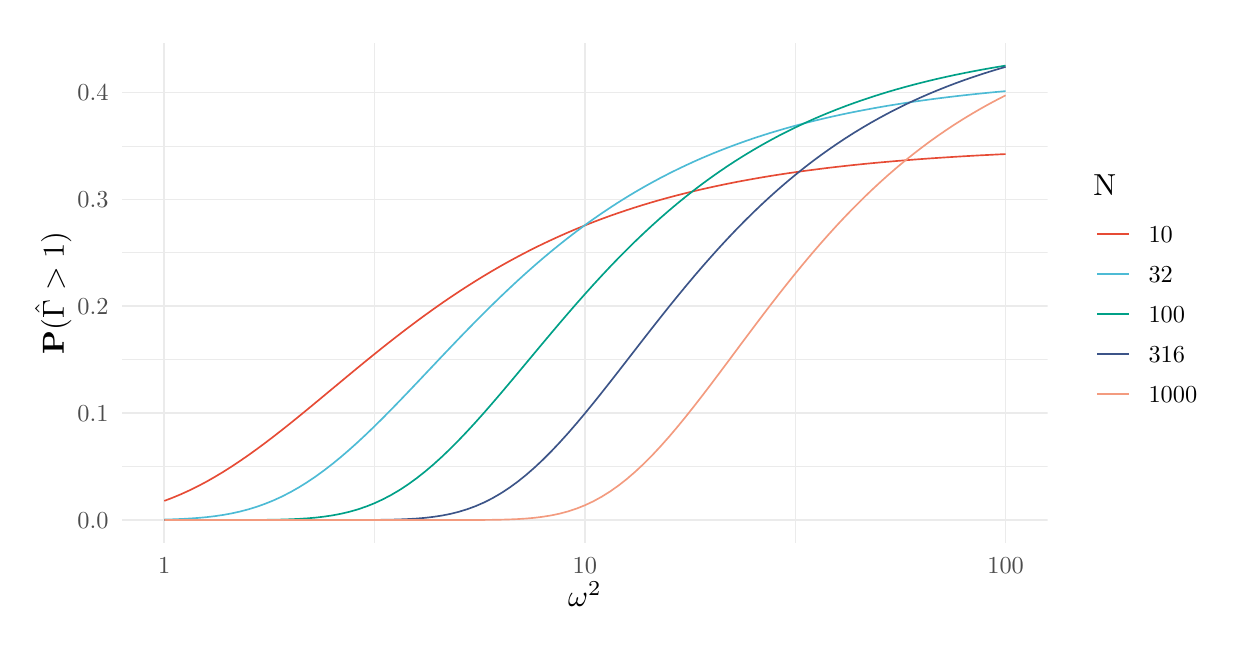
\begin{tikzpicture}[x=1pt,y=1pt]
\definecolor{fillColor}{RGB}{255,255,255}
\path[use as bounding box,fill=fillColor,fill opacity=0.00] (0,0) rectangle (433.62,216.81);
\begin{scope}
\path[clip] ( 34.16, 30.69) rectangle (368.57,211.31);
\definecolor{drawColor}{gray}{0.92}

\path[draw=drawColor,line width= 0.3pt,line join=round] ( 34.16, 58.20) --
	(368.57, 58.20);

\path[draw=drawColor,line width= 0.3pt,line join=round] ( 34.16, 96.82) --
	(368.57, 96.82);

\path[draw=drawColor,line width= 0.3pt,line join=round] ( 34.16,135.43) --
	(368.57,135.43);

\path[draw=drawColor,line width= 0.3pt,line join=round] ( 34.16,174.05) --
	(368.57,174.05);

\path[draw=drawColor,line width= 0.3pt,line join=round] (125.36, 30.69) --
	(125.36,211.31);

\path[draw=drawColor,line width= 0.3pt,line join=round] (277.37, 30.69) --
	(277.37,211.31);

\path[draw=drawColor,line width= 0.6pt,line join=round] ( 34.16, 38.90) --
	(368.57, 38.90);

\path[draw=drawColor,line width= 0.6pt,line join=round] ( 34.16, 77.51) --
	(368.57, 77.51);

\path[draw=drawColor,line width= 0.6pt,line join=round] ( 34.16,116.13) --
	(368.57,116.13);

\path[draw=drawColor,line width= 0.6pt,line join=round] ( 34.16,154.74) --
	(368.57,154.74);

\path[draw=drawColor,line width= 0.6pt,line join=round] ( 34.16,193.35) --
	(368.57,193.35);

\path[draw=drawColor,line width= 0.6pt,line join=round] ( 49.36, 30.69) --
	( 49.36,211.31);

\path[draw=drawColor,line width= 0.6pt,line join=round] (201.36, 30.69) --
	(201.36,211.31);

\path[draw=drawColor,line width= 0.6pt,line join=round] (353.37, 30.69) --
	(353.37,211.31);
\definecolor{drawColor}{RGB}{230,75,53}

\path[draw=drawColor,line width= 0.6pt,line join=round] ( 49.36, 45.81) --
	( 52.40, 46.97) --
	( 55.44, 48.24) --
	( 58.48, 49.62) --
	( 61.52, 51.12) --
	( 64.56, 52.73) --
	( 67.60, 54.46) --
	( 70.64, 56.28) --
	( 73.68, 58.21) --
	( 76.72, 60.23) --
	( 79.76, 62.33) --
	( 82.80, 64.52) --
	( 85.84, 66.77) --
	( 88.88, 69.09) --
	( 91.92, 71.46) --
	( 94.96, 73.88) --
	( 98.00, 76.34) --
	(101.04, 78.83) --
	(104.08, 81.34) --
	(107.12, 83.86) --
	(110.16, 86.39) --
	(113.20, 88.92) --
	(116.24, 91.44) --
	(119.28, 93.95) --
	(122.32, 96.44) --
	(125.36, 98.90) --
	(128.40,101.34) --
	(131.44,103.74) --
	(134.48,106.10) --
	(137.52,108.43) --
	(140.56,110.71) --
	(143.60,112.94) --
	(146.64,115.12) --
	(149.68,117.26) --
	(152.72,119.34) --
	(155.76,121.37) --
	(158.80,123.34) --
	(161.84,125.26) --
	(164.88,127.13) --
	(167.92,128.94) --
	(170.96,130.70) --
	(174.00,132.40) --
	(177.04,134.04) --
	(180.08,135.64) --
	(183.12,137.18) --
	(186.16,138.67) --
	(189.20,140.10) --
	(192.24,141.49) --
	(195.28,142.83) --
	(198.32,144.12) --
	(201.36,145.36) --
	(204.40,146.56) --
	(207.44,147.71) --
	(210.48,148.82) --
	(213.52,149.88) --
	(216.56,150.91) --
	(219.60,151.89) --
	(222.64,152.84) --
	(225.68,153.75) --
	(228.72,154.62) --
	(231.76,155.46) --
	(234.80,156.26) --
	(237.84,157.03) --
	(240.88,157.77) --
	(243.92,158.48) --
	(246.97,159.16) --
	(250.01,159.81) --
	(253.05,160.44) --
	(256.09,161.04) --
	(259.13,161.61) --
	(262.17,162.16) --
	(265.21,162.69) --
	(268.25,163.20) --
	(271.29,163.68) --
	(274.33,164.14) --
	(277.37,164.58) --
	(280.41,165.01) --
	(283.45,165.41) --
	(286.49,165.80) --
	(289.53,166.18) --
	(292.57,166.53) --
	(295.61,166.87) --
	(298.65,167.20) --
	(301.69,167.51) --
	(304.73,167.81) --
	(307.77,168.09) --
	(310.81,168.36) --
	(313.85,168.62) --
	(316.89,168.87) --
	(319.93,169.11) --
	(322.97,169.34) --
	(326.01,169.56) --
	(329.05,169.76) --
	(332.09,169.96) --
	(335.13,170.15) --
	(338.17,170.34) --
	(341.21,170.51) --
	(344.25,170.68) --
	(347.29,170.83) --
	(350.33,170.99) --
	(353.37,171.13);
\definecolor{drawColor}{RGB}{77,187,213}

\path[draw=drawColor,line width= 0.6pt,line join=round] ( 49.36, 39.07) --
	( 52.40, 39.15) --
	( 55.44, 39.27) --
	( 58.48, 39.44) --
	( 61.52, 39.65) --
	( 64.56, 39.93) --
	( 67.60, 40.29) --
	( 70.64, 40.74) --
	( 73.68, 41.29) --
	( 76.72, 41.96) --
	( 79.76, 42.76) --
	( 82.80, 43.69) --
	( 85.84, 44.78) --
	( 88.88, 46.01) --
	( 91.92, 47.41) --
	( 94.96, 48.97) --
	( 98.00, 50.70) --
	(101.04, 52.59) --
	(104.08, 54.64) --
	(107.12, 56.85) --
	(110.16, 59.20) --
	(113.20, 61.69) --
	(116.24, 64.31) --
	(119.28, 67.04) --
	(122.32, 69.88) --
	(125.36, 72.81) --
	(128.40, 75.82) --
	(131.44, 78.90) --
	(134.48, 82.03) --
	(137.52, 85.20) --
	(140.56, 88.39) --
	(143.60, 91.61) --
	(146.64, 94.82) --
	(149.68, 98.04) --
	(152.72,101.23) --
	(155.76,104.41) --
	(158.80,107.55) --
	(161.84,110.65) --
	(164.88,113.71) --
	(167.92,116.71) --
	(170.96,119.66) --
	(174.00,122.55) --
	(177.04,125.38) --
	(180.08,128.14) --
	(183.12,130.83) --
	(186.16,133.45) --
	(189.20,136.00) --
	(192.24,138.47) --
	(195.28,140.87) --
	(198.32,143.20) --
	(201.36,145.45) --
	(204.40,147.63) --
	(207.44,149.74) --
	(210.48,151.77) --
	(213.52,153.74) --
	(216.56,155.63) --
	(219.60,157.46) --
	(222.64,159.22) --
	(225.68,160.91) --
	(228.72,162.55) --
	(231.76,164.11) --
	(234.80,165.62) --
	(237.84,167.07) --
	(240.88,168.47) --
	(243.92,169.81) --
	(246.97,171.09) --
	(250.01,172.32) --
	(253.05,173.51) --
	(256.09,174.64) --
	(259.13,175.73) --
	(262.17,176.78) --
	(265.21,177.78) --
	(268.25,178.74) --
	(271.29,179.65) --
	(274.33,180.54) --
	(277.37,181.38) --
	(280.41,182.19) --
	(283.45,182.96) --
	(286.49,183.70) --
	(289.53,184.41) --
	(292.57,185.09) --
	(295.61,185.74) --
	(298.65,186.36) --
	(301.69,186.95) --
	(304.73,187.52) --
	(307.77,188.07) --
	(310.81,188.59) --
	(313.85,189.08) --
	(316.89,189.56) --
	(319.93,190.02) --
	(322.97,190.45) --
	(326.01,190.87) --
	(329.05,191.27) --
	(332.09,191.65) --
	(335.13,192.01) --
	(338.17,192.36) --
	(341.21,192.69) --
	(344.25,193.01) --
	(347.29,193.31) --
	(350.33,193.60) --
	(353.37,193.88);
\definecolor{drawColor}{RGB}{0,160,135}

\path[draw=drawColor,line width= 0.6pt,line join=round] ( 49.36, 38.90) --
	( 52.40, 38.90) --
	( 55.44, 38.90) --
	( 58.48, 38.90) --
	( 61.52, 38.90) --
	( 64.56, 38.90) --
	( 67.60, 38.90) --
	( 70.64, 38.90) --
	( 73.68, 38.90) --
	( 76.72, 38.91) --
	( 79.76, 38.92) --
	( 82.80, 38.93) --
	( 85.84, 38.96) --
	( 88.88, 39.00) --
	( 91.92, 39.07) --
	( 94.96, 39.17) --
	( 98.00, 39.31) --
	(101.04, 39.51) --
	(104.08, 39.77) --
	(107.12, 40.13) --
	(110.16, 40.58) --
	(113.20, 41.16) --
	(116.24, 41.87) --
	(119.28, 42.74) --
	(122.32, 43.77) --
	(125.36, 44.99) --
	(128.40, 46.40) --
	(131.44, 48.00) --
	(134.48, 49.80) --
	(137.52, 51.81) --
	(140.56, 54.01) --
	(143.60, 56.41) --
	(146.64, 58.99) --
	(149.68, 61.75) --
	(152.72, 64.66) --
	(155.76, 67.73) --
	(158.80, 70.92) --
	(161.84, 74.23) --
	(164.88, 77.63) --
	(167.92, 81.12) --
	(170.96, 84.67) --
	(174.00, 88.27) --
	(177.04, 91.90) --
	(180.08, 95.55) --
	(183.12, 99.20) --
	(186.16,102.84) --
	(189.20,106.46) --
	(192.24,110.05) --
	(195.28,113.60) --
	(198.32,117.10) --
	(201.36,120.53) --
	(204.40,123.91) --
	(207.44,127.21) --
	(210.48,130.45) --
	(213.52,133.60) --
	(216.56,136.67) --
	(219.60,139.66) --
	(222.64,142.56) --
	(225.68,145.38) --
	(228.72,148.11) --
	(231.76,150.75) --
	(234.80,153.31) --
	(237.84,155.78) --
	(240.88,158.17) --
	(243.92,160.47) --
	(246.97,162.69) --
	(250.01,164.83) --
	(253.05,166.89) --
	(256.09,168.87) --
	(259.13,170.77) --
	(262.17,172.60) --
	(265.21,174.36) --
	(268.25,176.05) --
	(271.29,177.68) --
	(274.33,179.24) --
	(277.37,180.73) --
	(280.41,182.16) --
	(283.45,183.54) --
	(286.49,184.86) --
	(289.53,186.12) --
	(292.57,187.33) --
	(295.61,188.49) --
	(298.65,189.60) --
	(301.69,190.66) --
	(304.73,191.68) --
	(307.77,192.65) --
	(310.81,193.59) --
	(313.85,194.48) --
	(316.89,195.33) --
	(319.93,196.15) --
	(322.97,196.93) --
	(326.01,197.68) --
	(329.05,198.40) --
	(332.09,199.08) --
	(335.13,199.74) --
	(338.17,200.36) --
	(341.21,200.96) --
	(344.25,201.53) --
	(347.29,202.08) --
	(350.33,202.60) --
	(353.37,203.10);
\definecolor{drawColor}{RGB}{60,84,136}

\path[draw=drawColor,line width= 0.6pt,line join=round] ( 49.36, 38.90) --
	( 52.40, 38.90) --
	( 55.44, 38.90) --
	( 58.48, 38.90) --
	( 61.52, 38.90) --
	( 64.56, 38.90) --
	( 67.60, 38.90) --
	( 70.64, 38.90) --
	( 73.68, 38.90) --
	( 76.72, 38.90) --
	( 79.76, 38.90) --
	( 82.80, 38.90) --
	( 85.84, 38.90) --
	( 88.88, 38.90) --
	( 91.92, 38.90) --
	( 94.96, 38.90) --
	( 98.00, 38.90) --
	(101.04, 38.90) --
	(104.08, 38.90) --
	(107.12, 38.90) --
	(110.16, 38.90) --
	(113.20, 38.90) --
	(116.24, 38.90) --
	(119.28, 38.91) --
	(122.32, 38.92) --
	(125.36, 38.94) --
	(128.40, 38.98) --
	(131.44, 39.03) --
	(134.48, 39.12) --
	(137.52, 39.25) --
	(140.56, 39.43) --
	(143.60, 39.69) --
	(146.64, 40.05) --
	(149.68, 40.51) --
	(152.72, 41.11) --
	(155.76, 41.87) --
	(158.80, 42.79) --
	(161.84, 43.91) --
	(164.88, 45.23) --
	(167.92, 46.77) --
	(170.96, 48.53) --
	(174.00, 50.52) --
	(177.04, 52.73) --
	(180.08, 55.17) --
	(183.12, 57.82) --
	(186.16, 60.67) --
	(189.20, 63.71) --
	(192.24, 66.93) --
	(195.28, 70.29) --
	(198.32, 73.80) --
	(201.36, 77.42) --
	(204.40, 81.14) --
	(207.44, 84.94) --
	(210.48, 88.79) --
	(213.52, 92.68) --
	(216.56, 96.60) --
	(219.60,100.52) --
	(222.64,104.44) --
	(225.68,108.33) --
	(228.72,112.18) --
	(231.76,116.00) --
	(234.80,119.75) --
	(237.84,123.44) --
	(240.88,127.06) --
	(243.92,130.60) --
	(246.97,134.06) --
	(250.01,137.44) --
	(253.05,140.72) --
	(256.09,143.91) --
	(259.13,147.01) --
	(262.17,150.01) --
	(265.21,152.92) --
	(268.25,155.73) --
	(271.29,158.45) --
	(274.33,161.07) --
	(277.37,163.60) --
	(280.41,166.04) --
	(283.45,168.39) --
	(286.49,170.65) --
	(289.53,172.82) --
	(292.57,174.91) --
	(295.61,176.92) --
	(298.65,178.85) --
	(301.69,180.70) --
	(304.73,182.48) --
	(307.77,184.18) --
	(310.81,185.82) --
	(313.85,187.39) --
	(316.89,188.89) --
	(319.93,190.33) --
	(322.97,191.71) --
	(326.01,193.03) --
	(329.05,194.29) --
	(332.09,195.50) --
	(335.13,196.66) --
	(338.17,197.77) --
	(341.21,198.83) --
	(344.25,199.85) --
	(347.29,200.82) --
	(350.33,201.75) --
	(353.37,202.64);
\definecolor{drawColor}{RGB}{243,155,127}

\path[draw=drawColor,line width= 0.6pt,line join=round] ( 49.36, 38.90) --
	( 52.40, 38.90) --
	( 55.44, 38.90) --
	( 58.48, 38.90) --
	( 61.52, 38.90) --
	( 64.56, 38.90) --
	( 67.60, 38.90) --
	( 70.64, 38.90) --
	( 73.68, 38.90) --
	( 76.72, 38.90) --
	( 79.76, 38.90) --
	( 82.80, 38.90) --
	( 85.84, 38.90) --
	( 88.88, 38.90) --
	( 91.92, 38.90) --
	( 94.96, 38.90) --
	( 98.00, 38.90) --
	(101.04, 38.90) --
	(104.08, 38.90) --
	(107.12, 38.90) --
	(110.16, 38.90) --
	(113.20, 38.90) --
	(116.24, 38.90) --
	(119.28, 38.90) --
	(122.32, 38.90) --
	(125.36, 38.90) --
	(128.40, 38.90) --
	(131.44, 38.90) --
	(134.48, 38.90) --
	(137.52, 38.90) --
	(140.56, 38.90) --
	(143.60, 38.90) --
	(146.64, 38.90) --
	(149.68, 38.90) --
	(152.72, 38.90) --
	(155.76, 38.90) --
	(158.80, 38.91) --
	(161.84, 38.92) --
	(164.88, 38.93) --
	(167.92, 38.97) --
	(170.96, 39.02) --
	(174.00, 39.11) --
	(177.04, 39.24) --
	(180.08, 39.43) --
	(183.12, 39.70) --
	(186.16, 40.08) --
	(189.20, 40.57) --
	(192.24, 41.21) --
	(195.28, 42.02) --
	(198.32, 43.02) --
	(201.36, 44.23) --
	(204.40, 45.66) --
	(207.44, 47.33) --
	(210.48, 49.23) --
	(213.52, 51.38) --
	(216.56, 53.77) --
	(219.60, 56.40) --
	(222.64, 59.24) --
	(225.68, 62.30) --
	(228.72, 65.56) --
	(231.76, 68.98) --
	(234.80, 72.57) --
	(237.84, 76.29) --
	(240.88, 80.12) --
	(243.92, 84.04) --
	(246.97, 88.03) --
	(250.01, 92.07) --
	(253.05, 96.14) --
	(256.09,100.23) --
	(259.13,104.31) --
	(262.17,108.36) --
	(265.21,112.39) --
	(268.25,116.37) --
	(271.29,120.30) --
	(274.33,124.15) --
	(277.37,127.94) --
	(280.41,131.64) --
	(283.45,135.26) --
	(286.49,138.78) --
	(289.53,142.21) --
	(292.57,145.55) --
	(295.61,148.78) --
	(298.65,151.91) --
	(301.69,154.95) --
	(304.73,157.88) --
	(307.77,160.71) --
	(310.81,163.45) --
	(313.85,166.08) --
	(316.89,168.62) --
	(319.93,171.06) --
	(322.97,173.42) --
	(326.01,175.68) --
	(329.05,177.85) --
	(332.09,179.93) --
	(335.13,181.94) --
	(338.17,183.86) --
	(341.21,185.70) --
	(344.25,187.47) --
	(347.29,189.17) --
	(350.33,190.79) --
	(353.37,192.35);
\end{scope}
\begin{scope}
\path[clip] (  0.00,  0.00) rectangle (433.62,216.81);
\definecolor{drawColor}{gray}{0.30}

\node[text=drawColor,anchor=base east,inner sep=0pt, outer sep=0pt, scale=  0.88] at ( 29.21, 35.87) {0.0};

\node[text=drawColor,anchor=base east,inner sep=0pt, outer sep=0pt, scale=  0.88] at ( 29.21, 74.48) {0.1};

\node[text=drawColor,anchor=base east,inner sep=0pt, outer sep=0pt, scale=  0.88] at ( 29.21,113.09) {0.2};

\node[text=drawColor,anchor=base east,inner sep=0pt, outer sep=0pt, scale=  0.88] at ( 29.21,151.71) {0.3};

\node[text=drawColor,anchor=base east,inner sep=0pt, outer sep=0pt, scale=  0.88] at ( 29.21,190.32) {0.4};
\end{scope}
\begin{scope}
\path[clip] (  0.00,  0.00) rectangle (433.62,216.81);
\definecolor{drawColor}{gray}{0.30}

\node[text=drawColor,anchor=base,inner sep=0pt, outer sep=0pt, scale=  0.88] at ( 49.36, 19.68) {1};

\node[text=drawColor,anchor=base,inner sep=0pt, outer sep=0pt, scale=  0.88] at (201.36, 19.68) {10};

\node[text=drawColor,anchor=base,inner sep=0pt, outer sep=0pt, scale=  0.88] at (353.37, 19.68) {100};
\end{scope}
\begin{scope}
\path[clip] (  0.00,  0.00) rectangle (433.62,216.81);
\definecolor{drawColor}{RGB}{0,0,0}

\node[text=drawColor,anchor=base,inner sep=0pt, outer sep=0pt, scale=  1.10] at (201.36,  7.64) {$\omega^2$};
\end{scope}
\begin{scope}
\path[clip] (  0.00,  0.00) rectangle (433.62,216.81);
\definecolor{drawColor}{RGB}{0,0,0}

\node[text=drawColor,rotate= 90.00,anchor=base,inner sep=0pt, outer sep=0pt, scale=  1.10] at ( 13.08,121.00) {$\mathbf P ( \hat \Gamma > 1 )$};
\end{scope}
\begin{scope}
\path[clip] (  0.00,  0.00) rectangle (433.62,216.81);
\definecolor{drawColor}{RGB}{0,0,0}

\node[text=drawColor,anchor=base west,inner sep=0pt, outer sep=0pt, scale=  1.10] at (385.07,156.09) {N};
\end{scope}
\begin{scope}
\path[clip] (  0.00,  0.00) rectangle (433.62,216.81);
\definecolor{drawColor}{RGB}{230,75,53}

\path[draw=drawColor,line width= 0.6pt,line join=round] (386.52,142.30) -- (398.08,142.30);
\end{scope}
\begin{scope}
\path[clip] (  0.00,  0.00) rectangle (433.62,216.81);
\definecolor{drawColor}{RGB}{77,187,213}

\path[draw=drawColor,line width= 0.6pt,line join=round] (386.52,127.84) -- (398.08,127.84);
\end{scope}
\begin{scope}
\path[clip] (  0.00,  0.00) rectangle (433.62,216.81);
\definecolor{drawColor}{RGB}{0,160,135}

\path[draw=drawColor,line width= 0.6pt,line join=round] (386.52,113.39) -- (398.08,113.39);
\end{scope}
\begin{scope}
\path[clip] (  0.00,  0.00) rectangle (433.62,216.81);
\definecolor{drawColor}{RGB}{60,84,136}

\path[draw=drawColor,line width= 0.6pt,line join=round] (386.52, 98.94) -- (398.08, 98.94);
\end{scope}
\begin{scope}
\path[clip] (  0.00,  0.00) rectangle (433.62,216.81);
\definecolor{drawColor}{RGB}{243,155,127}

\path[draw=drawColor,line width= 0.6pt,line join=round] (386.52, 84.48) -- (398.08, 84.48);
\end{scope}
\begin{scope}
\path[clip] (  0.00,  0.00) rectangle (433.62,216.81);
\definecolor{drawColor}{RGB}{0,0,0}

\node[text=drawColor,anchor=base west,inner sep=0pt, outer sep=0pt, scale=  0.88] at (405.02,139.27) {10};
\end{scope}
\begin{scope}
\path[clip] (  0.00,  0.00) rectangle (433.62,216.81);
\definecolor{drawColor}{RGB}{0,0,0}

\node[text=drawColor,anchor=base west,inner sep=0pt, outer sep=0pt, scale=  0.88] at (405.02,124.81) {32};
\end{scope}
\begin{scope}
\path[clip] (  0.00,  0.00) rectangle (433.62,216.81);
\definecolor{drawColor}{RGB}{0,0,0}

\node[text=drawColor,anchor=base west,inner sep=0pt, outer sep=0pt, scale=  0.88] at (405.02,110.36) {100};
\end{scope}
\begin{scope}
\path[clip] (  0.00,  0.00) rectangle (433.62,216.81);
\definecolor{drawColor}{RGB}{0,0,0}

\node[text=drawColor,anchor=base west,inner sep=0pt, outer sep=0pt, scale=  0.88] at (405.02, 95.91) {316};
\end{scope}
\begin{scope}
\path[clip] (  0.00,  0.00) rectangle (433.62,216.81);
\definecolor{drawColor}{RGB}{0,0,0}

\node[text=drawColor,anchor=base west,inner sep=0pt, outer sep=0pt, scale=  0.88] at (405.02, 81.45) {1000};
\end{scope}
\end{tikzpicture}
%
    }
    \caption{
        We show the probability that the estimated posterior variance $\hat \Gamma$ is bigger than the prior variance $1$ when varying the noise variance $\omega^{2}$. {\color{red} todo: ausführlicher beschreiben} %
        % for small N: N / N-1 difference in estimation
        % as omega grows, prob. increases
        % as N increases, larger omega necessary
    }
    \label{fig:ce_prob_failure}
\end{figure}

% all of these even worse if dimension grows
In higher-dimensional settings, e.g. when applying the \gls{cem} to \glspl{ssm}, we can expect this phenomenon to occur even more often. In the extreme case of independent marginals, i.e. when $\Sigma$ is a diagonal matrix, \Cref{eq:gamma_post} reduces to $(n + 1)p$ many decoupled equations, where $\hat \Gamma_{i,i}, i =1, \dots, (n + 1)p$ are independent. If all $q_{i} = \P \left(\Gamma_{i,i} > \Sigma_{i,i}\right)$ are identical to $q \in (0, 1)$, e.g. because $\Sigma$ and $\Omega$ are multiples of the identity, the number of failures follows a $\operatorname{Binom} \left( (n + 1)p, q \right)$ distribution, so that even small $q$ may lead to a non-negligible number of failures if the number of observations is high. 

% numerical scheme to solve eq.
Finally, in the multivariate setting, the system \eqref{eq:gamma_post} has no analytical solution. Instead, we have to resort to numerical methods to find a solution $\Omega$. Unfortunately, even evaluating the right-hand side of \eqref{eq:gamma_post} requires $\mathcal O(m^3)$ operations, as we have to invert $\Sigma + \Omega$. Additionally, we cannot hope to reuse a singular-value, LR, or eigenvalue-decomposition for further evaluations, as $\Sigma$ and $\Omega$ are not guaranteed to be jointly diagonalizable.
In the \gls{ssm} context we may use the Kalman-smoother to compute the marginal variances, but have to re-run the smoother for every evaluation. 

If we admit noise variance $\infty$ in the univariate setting, then $\Gamma > 1$ implies that the \gls{cem} chooses this as the estimate, i.e. $\G_{\hpce}$ is $\mathcal N(0, 1)$, which is equal to the prior. We can interpret this as having a missing observation, which, going back to the \gls{ssm} context, the Kalman-filter (\Cref{alg:kalman_filter}) can handle with only simple modifications, see e.g. \citep[Section 4.10]{Durbin2012Time}. However, if there are a lot of failures, the optimally chosen $\G_{\hpce}$ will be close to the prior distribution of states $X$, and importance sampling is unlikely to be effective. Hence, we turn to another approach that allows us to apply the \gls{cem} to \glspl{ssm}.

\subsection{The Markov-approach}
\label{subsec:markov-approach}
% second: Gaussian Markov process 
% discuss more flexible vs. fewer parameters
An alternative family of Gaussian proposals is given by directly modeling a Gaussian Markov process on the states $X_{:n}$. Again, this is sensible given the Markov structure of the target. This parametrization is more flexible than using the posterior of a \gls{glssm} with fixed prior as the proposal. This flexibility, however, comes at the cost of requiring a larger number of parameters. Here we propose with $\G_{\psi}$ where
\begin{align}
    \begin{split}
    \label{eq:markov-proposal}
    \G_{\psi} &= \mathcal L (U + v), \\
    v &\in \R^{(n + 1)m}, \\
    U_{0} &\sim \mathcal N(0, R_{0}R_{0}^T),\\
    U_{t} &= C_{t}U_{t - 1} + R_{t}\nu_{t}, \\
    C_{t} &\in \R^{m\times m},\\
    \nu_{t} &\sim \mathcal N(0,I_{m}), \\
    R_{t}&\in\R^{m \times m} \text{ lower triangular with positive diagonal}
    \end{split}
\end{align}
for $t = 1, \dots, n$, with $U_{0}$ and $\nu_{1}, \dots, \nu_{n}$ independent. The number of parameters in $$\psi= \left( v, C_{1}, \dots, C_{n}, R_{0}, \dots, R_{n} \right)$$ is $(n + 1)\cdot m$ for the mean $v$, $n \cdot m^{2}$ for the transition matrices $C_{t}$ and $(n + 1) \frac{m (m - 1)}{2}$ for the Cholesky roots of innovation covariances, totaling $\mathcal O(n\cdot m^{2})$ many parameters. 
While these are considerably more parameters than for the \gls{glssm}-approach for large state dimension $m$, we will see in the later part of this section that finding the optimal parameters for the \gls{cem} can be done analytically. 

This approach, which we term the \textbf{Markov-approach}, was originally proposed by \citep{Richard2007Efficient} for general unnormalized transition kernels as \gls{eis} proposals. However, because of its lower number of parameters, one should favor the \gls{glssm}-approach for \gls{eis} that operates on the signals, see \citep{Koopman2019Modified}.

To perform importance sampling with $\G_{\psi}$ in model \eqref{eq:markov-proposal} we not only need to simulate from $\G_{\psi}$ but also evaluate the unnormalized importance sampling weights $w(x) = \frac{p(x|y)}{g_{\psi}(x)}$. Simulation from $\G_{\psi}$ is achieved by a simple recursion. For the weights note that 
\begin{align}
\label{eq:weights_markov}
w(x) \propto \frac{p(y|x)p(x)}{g_{\psi}(x)} = \prod_{t = 0}^n \frac{p(y_{t}|x_{t})p(x_{t}|x_{t - 1})}{g_{\psi}(x_{t}|x_{t - 1})},
\end{align}
where $p(x_{0}|x_{-1}) = p(x_{0})$ and $g_{\psi}(x_{0}|x_{-1}) = g_{\psi}(x_{0})$.

The Markov structure of model \eqref{eq:markov-proposal} implies that the precision matrix of $\G_{\psi}$ is sparse, i.e. it has a block-tridiagonal form. This is a well-known property of the precision matrix of Gaussian random vectors, as the following two classical lemmas show. We show their proofs here for completeness. For a general treatment, we refer the reader to \citep[Chapters 3 and 5]{Lauritzen1996Graphical}.

\begin{lemma}
    \label{lem:gaussian_precision}
    Let $(X,Y)$ be jointly Gaussian with distribution $\mathcal N \left( \mu, \Sigma \right)$ where 
    $$
    \mu = \left(\mu_{X}, \mu_{Y}\right)
    $$
    and 
    $$
    \Sigma = \begin{pmatrix}
        \Sigma_{XX} & \Sigma_{XY} \\
        \Sigma_{YX} & \Sigma_{YY}
    \end{pmatrix},
    $$
    are partitioned according to the dimensions of $X$ and $Y$ and $\Sigma$ is non-singular.
    If $$P = \Sigma^{-1} = \begin{pmatrix} \Sigma_{XX} &  \Sigma_{XY} \\ \Sigma_{XY} & \Sigma_{YY} \end{pmatrix}^{-1}=  \begin{pmatrix} P_{XX} & P_{XY} \\ P_{YX} & P_{YY} \end{pmatrix}$$ 
    is the precision matrix of $(X,Y)$, partitioned as is $\Sigma$, then $\cov(X|Y) = P_{XX}^{-1}$.
\end{lemma}
\begin{proof}
    Without loss of generality, assume that both $X$ and $Y$ are centered. 
    The conditional density $p(x|y)$ is proportional (in $x$) to the joint density $p(x,y)$ with 
    $$\log p(x,y) = -\frac 1 2 \begin{pmatrix} x & y\end{pmatrix}  P \begin{pmatrix} x\\y\end{pmatrix} + C = -\frac 12 \left(x^TP_{XX}x + 2x^TP_{XY}y\right) + C',$$
    for constants $C, C'$ that do not depend on $x$. 
    As the conditional distribution of $X$ given $Y=y$ is Gaussian (by \Cref{lem:gaussian_conditional}), its covariance matrix is $P_{XX}^{-1}$.
\end{proof}

\begin{lemma}
    \label{lem:gaussian_precision_zeros}
    Let $(X,Y,Z) \sim \mathcal N \left( \mu, \Sigma \right)$ be jointly Gaussian with non-singular $\Sigma$. Then $X \perp Y | Z$ if, and only if, the sub-matrix of the precision matrix $P = \Sigma^{-1}$ whose rows correspond to the entries of $X$ and columns correspond to the entries of $Y$ is the $0$ matrix.
\end{lemma}
\begin{proof}
    Partition the conditional covariance matrix into
    $$
    \cov \left((X,Y) | Z\right) = \begin{pmatrix}
        \Sigma_{XX|Z} & \Sigma_{XY|Z} \\
        \Sigma_{YX|Z} & \Sigma_{YY|Z}
    \end{pmatrix}.
    $$

    As all distributions involved are Gaussian, $X \perp Y | Z$ is equivalent to $\cov \left( (X,Y) |Z \right)$ being a block-diagonal matrix with blocks $\Sigma_{XX|Z}$ and $\Sigma_{YY|Z}$, which is equivalent to its inverse being a block-diagonal matrix with blocks $\Sigma_{XX|Z}^{-1}$ and $\Sigma_{YY|Z}^{-1}$. Its inverse is, by \Cref{lem:gaussian_precision}, the sub-matrix of $P$ whose rows and columns correspond to $X$ and $Y$. 
\end{proof}

Applying \Cref{lem:gaussian_precision_zeros} to model \eqref{eq:markov-proposal}, we see that its precision matrix $P$ is sparse, i.e. it is a block-tri-diagonal matrix, as $U_{t} \perp U_{s} | U_{-t,-s}$ for $\lvert t - s\rvert > 1$ and $U_{-t,-s}$ being the vector of all $U_{0}, \dots, U_{n}$ except for $U_{t}, U_{s}$. Thus, the only entries of $P$ that are potentially non-zero are those whose row and column correspond to $(U_{t}, U_{t})$ for $t = 0, \dots, n$, $(U_{t}, U_{t - 1})$ and $(U_{t - 1}, U_{t})$ for $t=1, \dots, n$. 
Therefore, $P$ has the following block-tridiagonal structure:
\begin{align}
    \label{eq:P_structure}
P = \begin{pmatrix}
    P_{0,0} & P_{0, 1} & 0 & \cdots & \cdots & 0 & 0 \\
    P_{1, 0} & P_{1,1} & P_{1,2} & 0 & \cdots & 0 & 0\\
    0 & P_{2,1} & P_{2,2} & P_{2,3} & \cdots & 0 & 0 \\
    \vdots & \ddots & \ddots  & \ddots & \ddots & 0 & 0 \\
    0 & 0& 0& \cdots& P_{n - 1, n - 2}& P_{n - 1, n- 1} & P_{n - 1, n} \\
    0 & 0 & 0 & \cdots & 0 & P_{n, n - 1} & P_{n,n} 
\end{pmatrix}.
\end{align}
As the precision matrix is the natural parameter for the multivariate Gaussian exponential family, we see that model \eqref{eq:markov-proposal}, parameterized by $(P^{-1}v, P)$ form a natural exponential family and we can apply \Cref{thm:cem-clt} to obtain a central limit theorem when applying the \acrshort{cem} for this model. 

% show Cholesky root of precision matrix is also sparse -> Katzfuss (or refs therein), Lauritzen, Bernstein?, same as Schäfer paper?
The sparsity of $P$ implies that $P = LL^{T}$ has a sparse Cholesky root $L$, which will make computations efficient. 
To see that $L$ is sparse, we apply the following Theorem, slightly adapted to our notation, from the theory of Gaussian-Markov-Random-fields (GMRF), i.e. Gaussian models whose dependency structure is given by a graph, with edges between nodes indicating non-zero entries in the precision matrix.
\begin{theorem}[{\citep[Theorem 12.14]{Gelfand2010Discrete}}] 
    \label{thm:gelfand_gmrf}
    Let $X = (X_{0}, \dots, X_{n}) \in \R^{(n + 1)m}$ be a GMRF wrt to the labeled graph $G$, with mean $\mu$ and symmetric positive-definite precision matrix $P$. Let $L$ be the Cholesky factor of $P$ and define for $0 \leq t < s \leq n$ the future of $t$ except $s$ as 
    $$
        F(t,s) = \{t + 1, \dots, s - 1, s+ 1, n\}.
    $$
    Then
    $$
        X_{t} \perp X_{s} | X_{F(t,s)} \Leftrightarrow L_{t,s} = 0.
    $$
\end{theorem}
In the preceding theorem $X_{F(t,s)}$ is the vector of all $X_{u}$ for $u\in F(t,s)$ and $L_{t,s} \in \R^{m\times m}$ is the sub-matrix of $L$  whose rows correspond to $X_{t}$ and columns to $X_{s}$. 
From \Cref{thm:gelfand_gmrf} we immediately obtain the following:

\begin{corollary}[sparsity of $L$ in model \eqref{eq:markov-proposal}]
    \label{cor:sparsity_L}
    Let $U \sim \G_{\psi}$ as in \Cref{eq:markov-proposal}, $P \succ 0$ be the precision matrix of $\overset{\leftarrow}{U} = \left( U_{n}, \dots, U_{0} \right)$ and $L$ be the Cholesky root of $P$. 
    Then $L$ is a lower-block-diagonal matrix, with at most $n\,m^{2} + (n + 1)\,m\frac{m - 1}{2}$ non-zero entries:
    
    \begin{align}
        \label{eq:L_structure}
    L = \begin{pmatrix}
        L_{n,n} & 0 & \cdots & \cdots & \cdots & 0 & 0 \\
        L_{n-1, n} & L_{n-1,n-1} & 0 & \cdots & \cdots & 0 & 0\\
        0 & L_{n-2,n-1} & L_{n-2,n-2} & 0 & \cdots & 0 & 0 \\
        \vdots & \ddots & \ddots  & \ddots & \ddots & 0 & 0 \\
        0 & 0& 0& \cdots& L_{1, 2}& L_{1, 1} & 0 \\
        0 & 0 & 0 & \cdots & 0 & L_{0, 1} & L_{0,0} 
    \end{pmatrix},
    \end{align}
    where $L_{t,t} \in \R^{m\times m}, t = 0, \dots, n$ are lower triangular matrices with positive diagonal entries and $L_{t-1,t}\in\R^{m \times m}, t = 1, \dots, n$ are square matrices.
\end{corollary}

From $L$ in \Cref{cor:sparsity_L} we obtain an iterative method of sampling from $\G_{\psi}$: If $v + U \sim \G_{\psi}$, then, as $\cov U = \left( L L^{T} \right)^{-1} = L^{-T}L^{-1}$, it holds that $L^{T}U \sim \mathcal N(0, I)$ follows a standard normal distribution. Thus to simulate from $\G_{\psi}$ we may solve
$$
L^{T}U = \overset{\leftarrow} Z
$$
where $\overset{\leftarrow}Z = \left( Z_{n}, \dots, Z_{0} \right) \sim \mathcal N(0, I)$. Using the structure available in $L$, we see that this is equivalent to first solving
$$
L_{0,0}^T U_{0} = Z_{0}
$$
and then recursively solving for $t = 1, \dots, n$
$$
L_{t,t}^T U_{t} + L_{t-1, }^{T} U_{t-1} = Z_{t - 1}.
$$
Rearranging terms, provided $L_{t,t}$ is non-singular, we end up with the Markov-process
\begin{align}
\label{eq:rev_time_u}
    U_{t} = L^{-T}_{t,t} L_{t-1, t }^T U_{t - 1} +L^{-T}_{t,t} Z_{t},
\end{align}
where $Z_{t}$ is, by construction, independent of $U_{t - 1}$. Thus for model \eqref{eq:markov-proposal}, we obtain
\begin{align}
    \label{eq:parameters_markov_from_L}
    \begin{split}
    R_{t} &= L^{-T}_{t,t} \text{ for } t = 0, \dots, n,\\
    C_{t} &= L^{-T}_{t,t} L_{t-1, t }^T \text{ for } t =1, \dots, n.
    \end{split}
\end{align}
Here we see why we chose to use $\overset{\leftarrow}U$ in \Cref{cor:sparsity_L}: had we applied \Cref{thm:gelfand_gmrf} to $U$ directly we would have ended up with a Markov process in reverse time.

% show how to estimate Cholesky root analytically -> Schäfer
We now turn our attention to applying the \gls{cem} to model \eqref{eq:markov-proposal}. Following a similar argument as in the discussion surrounding \Cref{eq:cem_reparametrization}, we see that we may match the mean $v$ to that of $\P$ and it suffices to choose $P$, the precision matrix of $U$, such that it minimizes
\begin{align}
\label{eq:markov_ce_target}
\frac{1}{2} \operatorname{trace} \left( P \hat\Gamma \right) - \frac{1}{2}\log\det P
\end{align}
where $\hat\Gamma$ is the importance sampling estimate of the joint covariance matrix of all states $X$. This is equivalent to minimizing 
$$
\Dkl{\mathcal N(0,\hat\Gamma)}{\mathcal N(0, P^{-1})}.
$$
Here $P$ is restricted to precision matrices that may arise in model \eqref{eq:markov-proposal}, i.e., by \Cref{cor:sparsity_L}, $P = LL^{T}$ where $L$ possess structure as in \eqref{eq:L_structure}. 
At first glance, this problem seems more involved than solving \Cref{eq:gamma_post}: after all, the optimal $P$ depends on the whole covariance matrix $\hat\Gamma$. 
However, it turns out that the sparsity we enforce in $L$ allows us to compute analytically the optimal $\hat L$  that minimizes 
\Cref{eq:markov_ce_target}. Additionally, due to the Markov-structure of our proposal, $\hat L$ depends only on the block-tri-diagonal component of $\hat \Gamma$, i.e. only the covariances $\cov(X_{t}, X_{t-1})$ and $\cov (X_{0})$ are required. This is sensible - all information about the Markov transitions is encoded in these covariances if we assume that $X$ is a Gaussian Markov process.

To make this argument rigorous, let us apply the following result (stated in our notation).
\begin{theorem}[{\citep[Theorem 2.1]{Schafer2021Sparse}}]
    \label{thm:schafer_cholesky_analytical}
    Let $\Gamma$ be a positive-definite matrix of size $n\times n$. Given a lower-triangular sparsity set $S \subset \{1, \dots, n\}^{2}$, i.e. $i \geq j$ for all $(i,j) \in S$, let 
    $$
    \hat L = \argmin_{L \in \mathcal S} \Dkl{\mathcal N (0, \Gamma)}{\mathcal N \left( 0, (LL^{T})^{-1} \right)}
    $$
    be the Cholesky root of the closest Gaussian (wrt. the \gls{kld}) with sparsity $\mathcal S = \{A \in \R^{n \times n}: A_{i,j} \neq 0 \Rightarrow (i,j) \in S\}$. 

    Then the following holds:
    The nonzero entries of the $i$-th column of $\hat L$ are given by 
    
    \begin{align}
    \label{eq:schafer_gamma}
        L_{s_{i}, i} &= \frac{\Gamma_{s_{i}, s_{i}}^{-1} e_{1}}{\sqrt{e_{1}^{T}\Gamma_{s_{i}, s_{i}}^{-1} e_{1}}},
    \end{align}
    where $s_{i} = \{j : (i,j) \in \mathcal S\}$, $\Gamma_{s_{i}, s_{i}}$ is the restriction of $\Gamma$ to the set of indices $s_{i}$ and $e_{1} \in\R^{\lvert s_{i}\rvert}$ is the first unit vector.
\end{theorem}
Exploiting the Markov structure of our proposals, we immediately obtain the following:
\begin{corollary}
    \label{cor:markov_sparsity}
    Let $\mathcal S$ be the sparsity set of a Gaussian Markov process of the form \Cref{eq:markov-proposal}, i.e. 
    $$
        \mathcal S = \left\{ ((t,i),(s,j)) \in \left(\{0,\dots, n\}\times \{1,\dots, m\}\right)^{2} \,|\, (t = s \text{ and } i \geq  j) \text{ or } t = s + 1 \right\},
    $$
    see also \Cref{eq:L_structure},
    and let $\Gamma$ be a positive definite matrix of size $((n+1)m)\times(n + 1)m$ with blocks
    $$
        \Gamma_{s,t} = (\Gamma_{(s,i),(t,j)})_{i,j =1,\dots,m}.
    $$
    Then $\hat L$ in \Cref{thm:schafer_cholesky_analytical} depends only on the block-diagonal entries $\Gamma_{t, t}$, $ t = 0, \dots, n$ and block off-diagonal entries $\Gamma_{t, t + 1}$, $t = 0, \dots, n$.

    If, in particular, $\Gamma$ is the covariance matrix of Gaussian Markov process, $\hat L = \operatorname{chol} (\Gamma ^{-1})$.
\end{corollary}

We have thus shown the following: The covariance matrix of the KL-optimal Gaussian Markov process for the positive definite covariance matrix $\Gamma$ with $\mathcal O(n^{2}m^{2})$ entries only depends on $\mathcal O(n m^{2})$ many entries, the marginal covariances. In particular, if we can find a centered Gaussian Markov process $(X_{t})_{t = 0, \dots, n}$ whose marginal covariances fulfill 
\begin{align*}
    \cov (X_{t}) = \Gamma_{t}  && t = 0, \dots, n\\
    \cov (X_{t}, X_{t + 1}) = \Gamma_{t, t + 1} && t = 0, \dots, n,
\end{align*}
then its law $\mathcal L (X)$ is the one we seek. The following proposition puts all the pieces together.

\begin{proposition}[the \acrshort{cem} for the Markov proposal]
    \label{prop:cem-for-markov-proposal}
    Let $\P$ be a probability measure on $\R^{(n+1)\times m}$ with mean $\mu$ and positive definite covariance matrix $\Gamma$, partitioned into blocks 
    $$
        \Gamma_{s,t} = (\Gamma_{(s,i),(t,j)})_{i,j =1,\dots,m}.
    $$
    Let
    $$
        \begin{pmatrix}
            J_{t,t} & 0 \\
            J_{t + 1, t} & Z_{t+1, t+1}
        \end{pmatrix} = \operatorname{chol} \begin{pmatrix}
            \Gamma_{t,t} & \Gamma_{t, t + 1} \\
            \Gamma_{t + 1, t} & \Gamma_{t + 1, t + 1}
        \end{pmatrix}.
    $$

    Then the optimal cross-entropy parameter
    $$
        \pce = \argmin_{\psi = (v, C_{1}, \dots, C_{n}, R_{0}, \dots, R_{n})} \Dkl{\P}{\G_{\psi}}
    $$
    \todo{adapt notation to model? use tildes as cholesky roots}
    for the Markov proposal $\G_{\psi}$ from model \eqref{eq:markov-proposal} exists and is unique. The components of $\pce$ are given by 
    \begin{align*}
        v &= \mu\\
        R_{0} &= \operatorname{chol} (\Gamma_{0,0}) 
    \end{align*}
    and for $t = 1, \dots, n$
    \begin{align*}
        C_{t} &= J_{t + 1, t} J_{t, t}^{-1}\\
        R_{t} &= Z_{t + 1, t + 1}
    \end{align*}

    Thus, given $\nu$ and $\Gamma$, $\pce$ can be obtained in $\mathcal O(n\,m^{3})$ many operations.
\end{proposition}

\begin{proof}
    It only remains to show the uniqueness and existence of $\pce$, as well as its representation.
    The discussion surrounding \Cref{eq:markov_ce_target} shows that $v = \mu$ has to hold, so we may assume that $\P$ and the proposal are both centered.
    As $\Gamma$ is positive definite, so are all of its sub-matrices, and we may apply \Cref{cor:markov_sparsity}. Therefore, if we can show that there is a unique Gaussian Markovian probability measure whose covariance matrix matches $\Gamma$ as in that corollary we are done. 

    Let $(U_{t})_{t = 0, \dots, n} \sim \G_{\pce}$. Then 
    $$
        \cov (U_{0}) = R_{0}R_{0}^T = \Gamma_{0,0},
    $$
    and from the Cholesky decomposition we obtain for $t = 0, \dots, n - 1$
    $$
        \begin{pmatrix}
            J_{t,t}J_{t,t}^T & J_{t,t}J_{t + 1, t}^T\\
            J_{t +1, t}J_{t,t}^T & J_{t + 1, t}J_{t + 1, t}^{T} + Z_{t + 1, t + 1} Z_{t + 1, t + 1}^T.
        \end{pmatrix} = \begin{pmatrix}
            \Gamma_{t,t} & \Gamma_{t, t + 1} \\
            \Gamma_{t + 1, t} & \Gamma_{t + 1, t + 1}
        \end{pmatrix}.
    $$
    As $Z_{t + 1, t + 1}$ is a lower triangular matrix with positive diagonal and
    $$
        \Gamma_{t + 1, t + 1} - \Gamma_{t+1, t}\Gamma_{t}^{-1}\Gamma_{t, t +1} = Z_{t + 1, t + 1} Z_{t + 1, t + 1}^T,
    $$
    it is the Cholesky root of the Schur complement $\Gamma_{t + 1, t + 1} - \Gamma_{t+1, t}\Gamma_{t}^{-1}\Gamma_{t, t +1}$, which, recalling \Cref{lem:gaussian_conditional}, we can think of as a conditional covariance matrix. 
    Therefore, using induction over $t = 0, \dots, n - 1$, we obtain
    \begin{align*}
        \cov \left( U_{t + 1} \right) &= C_{t + 1}\cov \left( U_{t} \right) C^T_{t + 1} + R_{t + 1}R_{t + 1}^T \\
            &= J_{t + 1, t}J_{t,t}^{-1}\Gamma_{t,t}J_{t,t}^{-T}J_{t+1,t}^T + \Gamma_{t + 1, t + 1} - \Gamma_{t+1, t}\Gamma_{t}^{-1}\Gamma_{t, t +1}\\
            &= \Gamma_{t + 1, t + 1}
    \end{align*}
    and
    \begin{align*}
        \cov \left( U_{t + 1}, U_{t} \right) &= C_{t}\cov \left( U_{t} \right) = J_{t + 1, t}J_{t,t}^{-1} J_{t,t} J_{t, t}^T = \Gamma_{t + 1, t}.
    \end{align*}
    This shows the existence. For uniqueness, note that model \eqref{eq:markov-proposal} enforces that $R_{t}$ is a lower triangular matrix with positive diagonals. As $R_{t + 1}R_{t + 1}^T$ is the conditional covariance of $U_{t + 1}$ given $U_{t}$ which is, by \Cref{lem:gaussian_conditional} given by $\Gamma_{t + 1, t + 1} - \Gamma_{t + 1, t}\Gamma_{t,t}^{-1}\Gamma_{t + 1, t}$. Thus the $R$ matrices are unique as well. As $\cov (U_{t + 1}, U_{t}) = C_{t}\cov (U_{t})$, we can show that, additionally, also $C_{t}$ is unique.
\end{proof}

\todo{rewrite everything in terms of this prop}
When using the \acrshort{cem}, we do not have access to the mean and covariances necessary to apply this proposition. Instead, we may apply the \gls{cem} to estimate $\psi$ in model \eqref{eq:markov-proposal} by replacing these unknown moments with their importance sampling estimates. Given importance samples $U^{1}, \dots, U^{N}$ for $\mathcal L (X| Y = y)$ and associated auto-normalized weights $W^{1}, \dots, W^{N}$, we estimate $v$ by 
\begin{align}
\label{eq:hat_v}
\hat v = \sum_{i = 1}^N W^{i}X^{i}
\end{align}
and the empirical covariance matrices
\begin{align}
    \label{eq:empirical_covs}
    \begin{split}
    \widehat{\cov} \left( X_{t}, X_{t - 1} \right) &= \sum_{i = 1}^N W^{i}(X_{t:t-1}^{i} - \hat v_{t-1:t}) (X_{t:t-1}^{i} - \hat v_{t-1:t})^{T}\\
\widehat{\cov} \left( X_{0}\right) &= \sum_{i = 1}^N W^{i}(X_{0}^{i} - \hat v_{0}) (X_{0}^{i} - \hat v_{0})^{T}
    \end{split}
\end{align}
These steps are summarized in \Cref{alg:cem-markov-proposal}. 

\begin{algorithm}
    \caption{The \gls{cem} for the Markov proposal \eqref{eq:markov-proposal}}
    \label{alg:cem-markov-proposal}
    \begin{algorithmic}[1]
        \Require \gls{lcssm} (\Cref{def:lcssm}), observations $Y$, initial estimate $\hat\psi^0 = \left( v^{0}, C^{0}, R^{0}\right)$, sample size $N$
        \State set $l = 0$
        \Repeat 
            \State\label{step:cem-simulate} sample $U^{1} + v^{l}, \dots, U^{N} + v^{l} \iid \G_{\hat\psi^{l}}$ with fixed seed \Comment{\Cref{eq:markov-proposal}} 
            \State\label{step:cem-weights} determine auto-normalized weights $W^{1}, \dots, W^{N}$ \Comment{\Cref{eq:weights_markov}}
            \State\label{step:cem-est_v} estimate $\hat v^{l + 1}$ \Comment{\Cref{eq:hat_v}} 
            \State\label{step:cem-est_cov} estimate $\widehat{\cov} (U_{t}, U_{t-1}), t=1, \dots, n$, and $\widehat\cov (U_{0})$ \Comment{\Cref{eq:empirical_covs}}
            %\State\label{step:cem-L} determine $\hat L^{l + 1}$ \Comment{\Cref{thm:schafer_cholesky_analytical}}
            \State\label{step:cem-C_R} determine $C^{l + 1}$ and $R^{l + 1}$ \Comment{\Cref{prop:cem-for-markov-proposal}}
            \State\label{step:cem-est_phi} set $\hat\psi^{l + 1} = \left( \hat v^{l + 1}, C^{l + 1}, R^{l + 1}\right)$ 
            \State set $l = l + 1$
        \Until{$\hat\psi^{l}$ converged}
        \State \textbf{return} $\hpce = \hat \psi^{l}$
    \end{algorithmic}
\end{algorithm}

% initial value: could also use LA/EIS
To run \Cref{alg:cem-markov-proposal} we require an initial value for $\hat\psi^{0}$. If a suitable $\hat\psi^{0}$ is not available, we can obtain one from the \gls{la} by sampling $X^{1}, \dots, X^{N}$ from the \gls{la} and performing steps \ref{step:cem-est_v} to \ref{step:cem-est_phi} from the loop.
Alternatively, we could also directly base our initial value on the smoothing distribution of the \gls{glssm} that the \gls{la} is based on. The Kalman smoother (\Cref{alg:kalman_smoother}) provides us with the analytically available covariances $\cov \left( X_{t}, X_{t - 1} | Z = z \right)$ and the marginal covariance $\cov \left( X_{0} | Z = z \right)$ can be computed as well. 

% convergence: number of iterations, rel. change in psi
The convergence criteria in \Cref{alg:cem-markov-proposal} is similar to that used for \gls{eis}: we stop until the absolute or entry-wise relative difference of $\hat\psi^{l}$ and $\hat \psi^{l + 1}$ is smaller than a predetermined threshold, or a fixed number of iterations has passed. For the matrices involved, we use the Frobenius norm and the Euclidean distance for the mean $v$. 

In \Cref{step:cem-simulate} we use the standard praxis of \glspl{crn} to ensure numerical convergence. This is similar to \gls{eis} and the maximum likelihood estimates from \Cref{sec:maximum_likelihood_estimation}.

% runtime
We give an overview of the time and space complexities of each line in \Cref{alg:cem-markov-proposal} in \Cref{tab:cem-time-space-complexity}
The total time complexity of a single iteration of \Cref{alg:cem-markov-proposal} is $\mathcal O \left( N\,n\,m^{2} + n\,m^{3}\right)$ and its space complexity is $\mathcal O \left( N\,n\,m + n\,m^{2}\right)$. Let us elaborate on the complexities of each step:
\begin{enumerate}
    \item[\Cref{step:cem-simulate}] Generate $N$ i.i.d. samples from model \eqref{eq:markov-proposal}, where each simulation requires $\mathcal O(n)$ matrix-vector multiplications of dimension $m$. 
    \item[\Cref{step:cem-weights}] To evaluate the weights, \Cref{eq:weights_markov}, we have to evaluate for every sample $\mathcal O(n)$-times the density of a $m$-variate Gaussian distribution, while this usually has time-complexity $\mathcal O(m^{3})$, we have access to the Cholesky root $R_{t}$, so this step has only time-complexity $\mathcal O(m^{2})$. In \Cref{eq:weights_markov} we also need to compute $p(y_{t}|x_{t})$ and $p(x_{t}|x_{t - 1})$. Assuming conditional independence of observations, $p(y_{t}|x_{t}) = \prod_{i = 1}^{m}p(y_{t}^i|(B_{t}x_{t})^{i})$, evaluating the first term requires only $\mathcal O(m^{2})$ operations. For the second term, if we allow pre-computation of the Cholesky roots of innovations off-line (in $\mathcal O(m^{3})$ time), this step reduces to $\mathcal O(m^{2})$ as well.  
    \item[\Cref{step:cem-est_v}] Calculating the weighted mean $\hat v \in\R^{(n+1)m}$, \Cref{eq:hat_v}, requires $\mathcal O(N\,n\,m)$ operations.
    \item[\Cref{step:cem-est_cov}] Calculating the weighted covariance matrices, \Cref{eq:empirical_covs}, requires $(n+1)$ times multiplying $N$ many $m\times 1$ with $1 \times m$ vectors. 
    %\item[\Cref{step:cem-L}] To determine $L_{t,t}$ and $L_{t - 1, t}$ we have to solve $m$ times the linear systems of equations given in \Cref{eq:schafer_gamma}, where the dimension of the system is $2m,\dots, m + 1$. This requires $\mathcal O(m^{4})$ many operations, and we have to perform it for every one of the $n + 1$ time points. The result is $L$ with sparsity structure given by \Cref{eq:L_structure}, which has $\mathcal O (n m^{2})$ many non-zero entries.
    \item[\Cref{step:cem-C_R}] For each of the $\mathcal O(n)$ many $C_{t}$ and $R_{t}$ we have to calculate Cholesky decompositions and invert triangular matrices of dimension $m$. 
\end{enumerate}

\begin{table}
    \centering
    \begin{tabular}{lcc}
        \toprule
        step & time complexity & space complexity \\
        \midrule 
        simulation (\Cref{step:cem-simulate}) & $\mathcal O \left( N\,n\,m^{2}\right)$ & $\mathcal O \left( N\,n\,m \right)$\\
        weights (\Cref{step:cem-weights}) & $\mathcal O (N\,n\,m^{2})$ & $\mathcal O \left( N \right)$\\
        estimating $v$ (\Cref{step:cem-est_v}) & $\mathcal O (N\,n\,m)$ & $\mathcal O \left( n\,m \right)$\\
        estimating covariances (\Cref{step:cem-est_cov}) & $\mathcal O (N\,n\,m^{2})$ & $\mathcal O \left( n\,m \right)$\\
        determining $C$ and $R$ (\Cref{step:cem-C_R}) & $\mathcal O (n\,m^{3})$ & $\mathcal O (n\,m^{2})$\\
        \bottomrule
    \end{tabular}
    \caption{Time and space complexities of individual steps in \Cref{alg:cem-markov-proposal}.}
    \label{tab:cem-time-space-complexity}
\end{table}

An efficient implementation of \Cref{alg:cem-markov-proposal} can improve on the practically relevant computational time. There is no need to calculate the $C_{t}$ matrices explicitly, instead we can calculate $C_{t}U_{t - 1} = J_{t + 1, t}J_{t,t}^{-1}U_{t - 1}$ efficiently by back-substitution, as $J_{t,t}$ is a lower triangular matrix. 

% if space complexity is problematic, can compute weights first with fixed seed and then iterate forwards
The main bottleneck for space lies in the $\mathcal O(N\,n\,m)$ simulation part, and we may reduce this by simulating twice from model \eqref{eq:markov-proposal} using \glspl{crn}, and only storing the samples for a single time step (dimension $\mathcal O (N\,m)$) in each simulation. In the first pass, we only calculate the weights, and in the second pass, we calculate $\hat v$ and the required covariance matrices. For this, we only need the $2N$ samples of dimension $m$ from time $t$ and $t + 1$, i.e. $\mathcal O(N\,m)$ space. This reduces the total space complexity to $\mathcal O(N\,m + n\,m^{2})$. 

We demonstrate these improvements in \Cref{alg:cem-markov-proposal-fast}. Additionally, we calculate the weights on the log scale for numerical stability.

\begin{algorithm}
    \begin{algorithmic}[1]
        \Require \gls{lcssm} (\Cref{def:lcssm}), observations $Y$, initial estimate $\hat\psi^0 = \left( v^{0}, R^{0}, J^{0}\right)$, sample size $N$
        \State set $l = 0$
        \Repeat 
            \State simulate $\nu^{1}_0, \dots, \nu^{N}_0 \iid \mathcal N(0, I)$ 
            \State set $U^{i}_0 = R^{l}_{0}\nu_{0}^{i}$ 
            \State set $X_{0}^{i} = v^{l}_{0} + U^{i}_0$ 
            \State set $\log w^{i} = \log p(y_{0}|X_{0}^{i}) + \log p(X_{0}^i) + \frac{1}{2} \lVert \nu^{i}_0\rVert^{2}$ \Comment{$\log g(X_{0}^{i}) = -\frac{1}{2}\lVert \nu^{i}_{0}\rVert^{2}_2 + C$ }
            \State store current RNG state
            \For {$t \gets 1, \dots, n$}
                \State simulate $\nu^{1}_t, \dots, \nu^{N}_t \iid \mathcal N(0, I)$ 
                \State set $U^{i}_t = (J_{t + 1, t})^{T}(J_{t,t})^{-1}U^{i}_{t - 1} + R^{l}_{t}\nu_{t}^{i}$ \Comment{backsubstitution}
                \State set $X_{t}^{i} = v^{l}_{t} + U^{i}_t$ 
                \State set $\log w^{i} = \log w^{i} + \log p(y_{t}|X_{t}^{i}) + \log p(X_{t}^i|X_{t - 1}^i) + \frac{1}{2} \lVert \nu^{i}_t\rVert^{2}$ 
            \EndFor
            \State set $\log w^{i} = \log w^{i} - \max_{i = 1,\dots, N} \log w^{i}$ \Comment{ensure $\log w^{i} \leq 0$}
            \State set $w^{i} = \exp (\log w^{i})$
            \State set $W^{i} = \frac{w^{i}}{\sum_{i = 1}^N w^{i}}$ \Comment{auto-normalized weights}
            \State set $v^{l + 1}_0 = \sum_{i = 1}^{N}W^{i}X_{0}^i$
            \State restore RNG state
            \For {$t \gets 1, \dots, n$}
                \State simulate $\nu^{1}_t, \dots, \nu^{N}_t \iid \mathcal N(0, I)$ 
                \State set $U^{i}_t = (J_{t + 1, t})^{T}(J_{t,t})^{-1}U^{i}_{t - 1} + R^{l}_{t}\nu_{t}^{i}$ \Comment{backsubstitution}
                \State set $X_{t}^{i} = v^{l}_{t} + U^{i}_t$ 
                \State calculate $\hat v^{l + 1}_{t}$ \Comment{\Cref{eq:hat_v}}
                \State calculate covariances \Comment{\Cref{eq:hat_v}}
            \EndFor
            \State set $\hat\psi^{l + 1} = \left( \hat v^{l + 1}, \hat R^{l + 1}, \hat J^{l + 1}\right)$ 
            \State set $l = l + 1$
        \Until{$\hat\psi^{l}$ converged}
        \State \textbf{return} $\hpce = \hat \psi^{l}$
        
    \end{algorithmic}
    \caption{Time and space improved version of \Cref{alg:cem-markov-proposal}. Instructions involving the free index $i$ are to be performed for all $i = 1, \dots, N$ samples. For simplicity of notation we let $R^{l} = (R^{l}_0, \dots, R^{l}_n)$ and $J^l = (J^{l}_{0,0}, J^{l}_{1, 0}, \dots, J^{l}_{n - 1, n -1}, J^{l}_{n, n - 1} )$ for $l \in \N_{0}$.}
    \label{alg:cem-markov-proposal-fast}
\end{algorithm}

The advantage of \Cref{alg:cem-markov-proposal,alg:cem-markov-proposal-fast} over applying the \gls{cem} to the \gls{glssm} model \eqref{eq:glssm-proposal} are multiple: First of all, as long as the involved covariance matrices are positive definite, the two algorithms produce valid proposals, i.e. they do not have the degeneracy problem we observed in \Cref{subsec:glssm-approach}. When matrices are only positive-semi definite, replacing inverses with generalized inverses still yields a valid model.
% no numerical issues w/ determining optimal parameters
Additionally, determining the optimal parameters $(v, C,R)$ or $(v,J,R)$ is numerically stable, involving only inversion of small matrices. Compare this with solving \Cref{eq:gamma_post}, where we need to employ a numerical scheme to solve for the diagonal entries of $\Omega$.

% sampling faster 
After having determined $\hpce$ for model \eqref{eq:markov-proposal}, generating $N$ samples requires only $\mathcal O(N\,n\,m^{2})$ operations, whereas sampling from model \eqref{eq:glssm-proposal} requires $\mathcal O(n\,m^{3} + N\,n\,m^{2})$ operations, as we need an initial run of the Kalman filter. Unless $N < m$, this difference is negligible, and the case where $N < m$ is not really of interest, as we would expect importance sampling to require a much larger number of samples, i.e. $N \gg m$. 

% problems: large state dimension: both $L$ and number of parameters
However, the two algorithms presented in this section also come with some drawbacks, especially if the dimension $m$ of states is large. This affects the algorithms in multiple ways: when $m$ is large, computation of the Cholesky decomposition in \Cref{prop:cem-for-markov-proposal} becomes more time-intensive. Additionally, the dimension of the parameter $\psi$ increases quadratically in $m$, so we expect convergence to be slower, requiring a larger sample size $N$ to find the optimal $\hpce$. For an empirical study in this direction, see \Cref{sec:simulation_studies}.
%
\section{Accouting for multimodality and heavy tails}
\label{sec:accouting_for_multimodality_and_heavy_tails}
Performing importance sampling with the Gaussian models discussed so far will work well only if the smoothing distribution  $p(x|y)$ is well approximated by a Gaussian distribution. However, a Gaussian distribution is a very specific kind of distribution, in particular, it is an unimodal distribution
%that is constant on elliptical contours 
and has light tails \todo{check for correct wording}.

If the smoothing distribution violates any of these assumptions, importance sampling with the models presented so far is likely to fail, i.e. requiring large sample sizes for both finding the optimal importance sampling parameter $\hat \psi$ as well as the final importance sampling evaluation.

There are however techniques to keep most of the computational efficiency discussed in the above sections to address both multimodality as well as heavy tails.

We start with heavier than gaussian tails: the textbook example of a heavy tailed distribution is the multivariate $t$-distribution with density
$$
    \dots .
$$
for degrees of freedom  $\nu > 1$ \todo{?}, location $\mu$ and scale matrix $\Sigma$. When $\nu > 2$ then this distribution has mean $\mu$ and if $\nu > 3$ it has covariance matrix $?$ \todo{check}.

The main properties necessary to facilitate Gaussian importance sampling strategies above are that the distribution $p(x|y)$ is analytically tractable and simulation from it is possible. These properties still hold for the multivariate $t$-distribution and, in fact, for the even larger class of elliptical distributions:

\begin{theorem}[Conditional distribution of elliptical distributions]
    \label{thm:elliptical-conditional}
    \todo{cite the correct book}
\end{theorem}

As one can readily see from \Cref{thm:elliptical-conditional} the parameters of the smoothing distribution $p(x|y)$ if $p(x,y)$ follows an elliptical distribution is again elliptical and its parameters only depend on quantities that are computed by the Kalman smoother. \todo{elaborate}

\todo{present some models with heavy tails}


\section{Maximum likelihood estimation in SSMs}
\label{sec:maximum_likelihood_estimation}

% region introduction
%% need for MLE: hyperparameters
Until now, we have assumed that the \acrshort{ssm} under consideration is completely known, i.e. we have access to the true transition and observation kernels. For the models considered in this thesis (\Cref{cha:analysis_of_selected_models}), this is unrealistic, as they are not based on concrete physical processes but are rather statistical approximations of the true underlying dynamics. The transition densities of, e.g., \Cref{eq:glssm_states} will depend on the covariance matrix of innovations, of which we have no a priori knowledge and for negative binomially distributed observations the overdispersion parameter $r$ will be unknown. Let us denote by $\theta\in\R^{l}$ the vector of these hyperparameters. \todo{check l / k with psis}
To make this dependence explicit, we will introduce subscripts $\theta$ where appropriate, i.e. $\P_{\theta}$ is a target distribution that additionally depends on $\theta$, $p_{\theta}$ its density et cetera. This section is loosely based on \citep[Chapter 7 \& 11]{Durbin2012Time} and \citep[Chapter 14]{Chopin2020Introduction}

To determine a suitable value of $\theta$, multiple options are available. Here, we opt for a frequentist approach, using maximum likelihood estimation to determine an optimal $\hat \theta$. Therefore, given observations $y\in\R^{(n+1)\times p}$, $\hat\theta$ maximizes the likelihood $p_{\theta}(y)$ and can be obtained as the global maximum of the following optimization problem: 
$$
    \max_{\theta \in \Theta} p_{\theta}(y).
$$
For numerical stability, we should maximize the log-likelihood instead, i.e. solve 
\begin{align}
    \label{eq:max-log-p}
    \max_{\theta \in \Theta} \log p_{\theta}(y).
\end{align}
Here $\Theta \subseteq \R^{l}$ is the parameter space. To solve this optimization problem using gradient ascent algorithms, we need access to both the likelihood and its derivatives. Thus, in the following, we will assume that $\theta \mapsto \log p_{\theta}(y)$ is sufficiently smooth, to apply these methods, i.e. it has continuous derivatives of second order. 

%% GLSSM analytically available, still need to use gradient descent algs. 
%% analytically impossible
%% high dimensional integral -> importance sampling
While the Kalman-filter (\Cref{alg:kalman_filter}) allows analytical computation of this likelihood \acrshortpl{glssm}, in general \acrshortpl{ssm} it is numerically intractable. The reason for this is that
$$
    p_{\theta}(y) = \int p_{\theta}(x,y) \mathrm d \mu(x)
$$
is a high-dimensional integral, which is hard to evaluate numerically. Instead, we will use importance sampling to estimate the likelihood. For this, let us regard $p_{\theta}(x,y)$ as an unnormalized density in $x$. The missing integration constant is then just $p_{\theta}(y)$ and the normalized density is $p_{\theta}(x|y)$. If $\G \gg \P$ is a proposal distribution whose density $g$ with respect to $\mu$ we can evaluate analytically, i.e. not only up to a constant, we see that for the unnormalized weights $\tilde w_{\theta}(x) = \frac{p_{\theta}(x,y)}{g(x)}$, that $p_{\theta}(y) = \G [\tilde w_{\theta}]$. Thus we may estimate the likelihood by 
$$
    \verywidehat{p_{\theta}(y)} = \frac{1}{N}\sum_{i = 1}^N \tilde w_{\theta} (X^{i})
$$
for $X^{1}, \dots, X^{N} \iid \G$ and $N \in \N$. To evaluate the gradient, notice that as $\nabla_{\theta} p_{\theta}(x,y) = p_{\theta}(x,y) \nabla_{\theta} \log p_{\theta}(x,y)$, we have, provided we can exchange integration and differentiation,
\begin{align*}
     \nabla_{\theta} p_{\theta}(y) &= \nabla_{\theta}\int p_{\theta}(x,y)\d \mu(x) = \int p_{\theta}(x,y) \nabla_{\theta} \log p_{\theta}(x,y)\d \mu(x) \\
     &= \G [\tilde w_{\theta} \nabla_{\theta} \log p_{\theta}(x,y)],
\end{align*}
and so we may estimate the gradient by 
\begin{align*}
    \verywidehat{\nabla_{\theta} p_{\theta}(y)} &= \frac{1}{N}\sum_{i = 1}^N \tilde w_{\theta}(X^{i}) \nabla_{\theta} \log p_{\theta}(X^{i}, y)
    %&= \sum_{i = 1}^N \tilde w_{\theta}(X^{i}) \sum_{t = 0}^n \nabla_{\theta} \left( \log p_{\theta}(y_{t} | X^{i}_{t}) + \log p_{\theta}(X^{i}_t|X^{i}_{t - 1}) \right).
\end{align*}
Similarly, we can estimate the log-likelihood by Plug-In
\begin{align}
    \label{eq:loglik-hat-standard}
    \verywidehat{\log p_{\theta}(y)} = \log \left( \frac{1}{N}\sum_{i = 1}^N \tilde w_{\theta}(X^{i}) \right)
\end{align}
and its gradient, using the fact that the gradient of $\log f$ for $f: \R^{l} \to \R$ is $ \frac{1}{f} \nabla_{\theta} f$, by 
\begin{align*}
    \verywidehat{\nabla_{\theta} \log p_{\theta}(y)} &= \left(\frac{1}{N} \sum_{i = 1}^N \tilde w_{\theta}(X^{i}) \right)^{-1} \left( \frac{1}{N}\sum_{i = 1}^N \tilde w_{\theta}(X^{i}) \nabla_{\theta} \log p_{\theta}(X^{i}, y) \right) \\
    &=\sum_{i = 1}^N W_{\theta}^{i} \nabla_{\theta} \log p_{\theta}(X^{i}, y)
\end{align*}
where $W_{\theta}^{i} = \frac{\tilde w_{\theta}(X^{i})}{\sum_{i= 1}^N \tilde w_{\theta}(X^{i})}$ are the auto-normalized weights.
Note that, by Jensen's inequality, these estimates are biased.


%% optimizatino using CRNs, advantage over particle filters
To solve the optimization problem \eqref{eq:max-log-p} we will again employ \acrshortpl{crn}. If the densities involved are twice differentiable, this device ensures that the random objective function $\theta \mapsto \sum_{i = 1}^N \tilde w_{\theta}(X^{i})$ is twice differentiable, and so we can indeed apply gradient ascent to find a local maximum. This is an advantage of performing global importance sampling over \acrshort{smc}, i.e. particle filter, methods. To avoid collapse to a single particle, \acrshort{smc} methods perform intermediate resampling steps, which make the objective function discontinuous. While particle smoothing methods can mitigate this problem, they are more expensive than standard \acrshort{smc} and, as the importance sampling estimates of the log-likelihood and its gradient are biased, the usual requirements for stochastic approximation methods are not fulfilled. 
For a more thorough discussion of the challenges maximum likelihood estimation with \acrshort{smc} methods faces, we recommend \citep[Chapter 14]{Chopin2020Introduction}.

%% discuss not really frequentist setting
While \acrshortpl{mle} have a strong frequentist foundation, let us stress that, for the models that we investigate in \Cref{cha:analysis_of_selected_models}, the frequentist properties of the estimates are not of interest. The reason for this is that a frequentist interpretation requires us to imagine, at least hypothetically, an infinite repetition of the data-generating process. For the data at hand, such repetition is nonsensical: the pandemic is a \glqq{}one-off\grqq{} event that will not be replicated under even approximately similar circumstances. Therefore, we will choose to view the estimation procedure more as a hyper-parameter tuning step, rather than true frequentist inference. While we can compute asymptotic confidence intervals for $\hat\theta$, see, e.g., \citep[Chapter 11.6]{Durbin2012Time}, \citep[Chapter 14.8]{Chopin2020Introduction}, these are not of practical interest for similar reasons. 

%% alternative: fully Bayesian
As an alternative to modeling $\theta$ as fixed, but unknown, and performing maximum-likelihood estimation to obtain $\hat \theta$, one might also model $\theta$ as random with prior density $p(\theta)$, such that the full model becomes $p(x,y,\theta) = p(x,y|\theta)p(\theta)$. In this setup, sometimes called the Bayesian treatment of \acrshortpl{ssm} \citep[Section 13.1]{Durbin2012Time}, the main interest still lies in the posterior density $p(x,\theta|y)$, which, depending on the model at hand, can drastically increase the difficulty of the problem: even if $p(x,y|\theta)$ is an analytically tractable model such as a \acrshort{glssm}, unless the prior is chosen to be conjugate, one has to resort to, e.g., \acrshort{mcmc}-methods. 

% endregion

% region GLSSM proposal

%% joint density easy to calculate
By the structure of the model, \Cref{eq:joint_density}, the log density and its gradient can be computed efficiently by
\begin{align*}
    \log p_{\theta}(x,y) &= \log p_{\theta}(x_{0}) + \sum_{t = 1}^{n} \log p_{\theta}(x_{t}|x_{t-1}) + \log p_{\theta} (y_{t}|x_{t},y_{t - 1})\\
    \nabla_{\theta}\log p_{\theta}(x,y) &= \nabla_{\theta}\log p_{\theta}(x_{0}) + \sum_{t = 1}^{n} \nabla_{\theta}\log p_{\theta}(x_{t}|x_{t-1}) + \nabla_{\theta}\log p_{\theta} (y_{t}|x_{t},y_{t - 1}),
\end{align*}
respectively. 

Similarly, when proposing with a \acrshort{glssm} or Markov-proposal for a \acrshort{pgssm}, the weights have similar structure, see\Cref{eq:weights_markov,eq:weights_only_on_signal}, which makes calculation of $\tilde w$ efficient. 

For the remainder of this section, let us consider the \acrshort{glssm}-proposal obtained by \acrshort{eis} for a \acrshort{pgssm} with linear signal, as this is the main setting of \Cref{cha:analysis_of_selected_models}. For this we obtain 
$$
    \tilde w_{\theta}(x) = \tilde w_{\theta}(s) g(z)\frac{p_{\theta}(y|s)}{g(z|s)} = g(z) \prod_{t = 0}^n \frac{p_{\theta}(y_{t}|s_{t})}{g(z_{t}|s_{t})},
$$
where $s_{t} = B_{t}x_{t}$, $t = 0, \dots, n$, is the signal, and so the log-likelihood is given by 
\begin{align}
    \label{eq:loglik-pgssm-exact}
    \log p_{\theta}(y) = \log g_{\theta}(z) + \log \E \left(w_{\theta}(S)|Y = y\right)
\end{align}
and can be estimated by
\begin{align}
    \label{eq:loglik-hat-linearsignal}
    \verywidehat{\log p_{\theta}(y)} = \log g_{\theta}(z) + \log \left(\frac{1}{N}\sum_{i=1}^{N}\prod_{t = 0}^{n} \frac{p_{\theta}(y_{t}|S^{i}_{t})}{ g(z_{t}|S^{i}_{t})}\right).
\end{align}
Notice that $\log g_{\theta}(z)$ is the likelihood in a \acrshort{glssm}, which can be computed efficiently by the standard Kalman filter (\Cref{alg:kalman_filter}). As in the \acrshort{glssm}-approach we propose with an \acrshort{glssm} whose state density $g(x)$ and observation matrices $B_{t}$, $t = 0, \dots, n$ are equal to those of the target, the log-likelihood $\log g_{\theta}(z)$ also depends on $\theta$. The estimated gradient of the log-likelihood is 
$$
    \verywidehat{\nabla_{\theta} \log p_{\theta}(y)} = \nabla_{\theta} \log g_{\theta}(z) + \sum_{i=1}^N W^{i}_\theta \sum_{t = 0}^n \nabla_{\theta} \log p_{\theta}(y_{t}|S_{t}^{i}).
$$
The gradient of the \acrshort{glssm} log-likelihood can be obtained either numerically or analytically by employing the Kalman filter and smoother \citep{Koopman1992Exact}, however, numerical evaluation may be faster if the dimension of $\theta$ is small compared to the length of the time series, as evaluating the likelihood only requires a single application of the Kalman filter. 

As the observation densities $g(z_{t}|s_{t})$ do not depend on $\theta$, their derivatives do not appear in the above estimate. However, when using \acrshort{eis} to determine an optimal proposal, the parameter $\psi = (z, \omega)$ implicitly depends on $\theta$. Accounting for this yields the gradient 
$$
    \verywidehat{\nabla_{\theta} \log p_{\theta}(y)} = \nabla_{\theta} \log g_{\theta}(z) + \sum_{i=1}^N W^{i}_\theta \left(\sum_{t = 0}^n \nabla_{\theta} \log p_{\theta}(y_{t}|S_{t}^{i}) - \nabla_{\theta} \log g_{\theta}(z_{t}|S^{i}_{t})\right),
$$
as $\nabla_{\theta} \frac{1}{g_{\theta}(z|s)} = - \frac{1}{g_{\theta}(z|s)} \nabla_{\theta} \log g_{\theta}(z|s)$. The computation of this additional term is much more involved, as the parameters $z,\Omega$ are found through an iterative numerical scheme. Instead, we favor numerical differentiation of the whole procedure to evaluate the likelihood at $\theta$, including the method of finding an optimal importance sampling scheme. 


As a single evaluation of the log-likelihood can become very expensive we want our procedure to be as efficient as possible. To this end, \citep{Durbin1997Monte} provides several improvements to the basic algorithm if the model is a \acrshort{pgssm} with a linear signal. Their contributions consist of a bias correction for the log-likelihood, the use of antithetic and control variables to reduce Monte-Carlo error for importance sampling and a deterministic initialization procedure.
Let us briefly summarize these ideas, adapted to our notation. As the computational gains for control variates in the presence of antithetic variables seem to be limited, we do not give the same level of detail here, for an in-depth analysis, we refer the reader to the source. 

% bias reduction
For bias reduction, a second-order Taylor series expansion shows that for $\tilde{w}_\cdot = \frac{1}{N} \sum_{i =1}^N \tilde w(X^{i})$,
\begin{align*}
    \E \left(\log \tilde{w}_\cdot\right) - \log \G \tilde w &= \E \log \left(1 + \frac{\tilde{w}_\cdot - \G \tilde w}{\G \tilde w} \right)\\
                                                           &=  \frac{\tilde{w}_\cdot - \G \tilde w}{\G \tilde w}  - \frac{1}{2} \left(\frac{\tilde{w}_\cdot - \G \tilde w}{\G \tilde w} \right)^{2} + \mathcal O_{p}(N^{-\frac{3}{2}}),
\end{align*}
provided $\tilde w \in L^{3}(\G)$. Thus, estimating the second order term by $- \frac{\hat\sigma^2}{2N \tilde{w}_\cdot} $, where $\hat \sigma^{2}$ is the empirical variance of the unnormalized weights, we can perform a bias reduction by estimating 
\begin{align}
    \label{eq:loglik-hat-bias-reduction}
    \widehat{\log p_{\theta}(y)} = \log \left(\tilde w_{\cdot}\right) + \log g_{\theta}(z) + \frac{\hat\sigma^{2}}{2N\tilde w_{\cdot}}
\end{align}

% antithetics
The second improvement of \citep{Durbin1997Monte} is the use of antithetic variables and control variates, a device to reduce Monte-Carlo variance. The main idea of an antithetic variable is to construct for each sample $X^{i}$, $i = 1,\dots, N$, another sample $\tilde X^{i}$ that has the same distribution as $X^{i}$, but is negatively correlated with $X^{i}$. This has two effects: first of all, we increase the number of samples used for importance sampling and second, as the new samples are negatively correlated with the old samples, the Monte-Carlo variance is reduced. The computation of these samples is usually much faster than creating new samples, which requires the use of the expensive \acrshort{ffbs} or simulation smoother algorithms. 
\begin{definition}[antithetic variable]
    Let $X, \tilde X\in\R^{k}$ be two random variables with the same distribution, $\mathcal L (X) = \mathcal L(\tilde X)$ and $f: \R^{k} \to \R$. Then $\tilde X$ is called an antithetic variable of $X$ for $f$, if $\cov \left( f(\tilde X), f(X) \right) < 0$. If $k = 1$ and $f$ is the identity, we just say that $\tilde X$ is an antithetic variable of $X$.
\end{definition}

% location & scale
\citep{Durbin1997Monte} introduce two antithetic variables: balanced for location and balanced for scale, both of which are tailored to the multivariate normal distribution. 
\begin{definition}[antithetic variable balanced for location and scale, \citep{Durbin1997Monte}]
    Let $X\sim \mathcal N(\mu, \Sigma)$ for $\mu \in \R^{k}$ and $\Sigma \in \R^{k\times k}$ positive definite. We call
    \begin{align}
        \label{eq:antithetic-location}
    \tilde X = \mu + (\mu - X)
    \end{align}
    the antithetic balanced for location. If $L\in\R^{k\times k}$ is a Cholesky root of $\Sigma$ and 
    $$
        X = \mu + L \varepsilon
    $$
    with $\varepsilon \sim \mathcal N(0, I)$, let $c = \varepsilon^{T}\varepsilon \sim \chi^{2}_k$ and $c' = F^{-1}_{\chi^{2}_{k}}(1 - F_{\chi^{2}_k}(\sqrt{c}))$. We call
    \begin{align}
        \label{eq:antithetic-scale}
        \check X = \mu + \sqrt{\frac{c'}{c}} \left( X - \mu \right)
    \end{align}
    the antithetic balanced for location.
\end{definition}
\begin{lemma}
    In the above definition, $\tilde X_{i}$ is an antithetic variable of $X$ for the coordinate functions $f_{i}:\R^{k} \to \R$, $f_{i}(x) = x_{i}$, $i = 1, \dots, k$.
    Furthermore, $\tilde c$ is an antithetic variable of $c$.
\end{lemma}
\begin{proof}
    It is easy to see that $\tilde X$ has the same distribution as $X$. Furthermore 
    $$
        \cov \left( f_{i}(X), f_{i}(\tilde X)\right) = \cov \left( 2 \mu_{i} - X_{i}, X_{i} \right) = - \Sigma_{i,i} < 0.
    $$

    For $c$ and $\tilde c$, let $U = F_{\chi^{2}_{k}}(c)$, then $U \sim \operatorname{Unif}(0,1)$ and $\tilde U = 1 - U = F_{\chi^{2}_k}(\tilde c)$. 
    As $\tilde U \sim \operatorname{Unif}(0, 1)$ as well, $\mathcal L (c) = \mathcal L (\tilde c)$.
    In \citep[Lemma 2.3]{Whitt1976Bivariate} it is shown that for any pair of real-valued random variables $(Y,W)$ with CDF $H$ and marginal CDFs $F, G$, it holds
    $$
        \cov \left(Y,W \right) = \int_{\R^{2}} H(y,w) - F(y)G(w) \d y \d w,
    $$
    and, furthermore, by \citep[Theorem 2.1 and Lemma 2.4]{Whitt1976Bivariate} that the joint CDF of $(c, \tilde c)$ is $(y,w) \mapsto \max \{0, F(y) + G(w) - 1\}$, where $F$ is the CDF of $c$ and $G$ the CDF of $\tilde c$. 
    As 
    $$
        a + b - 1 = ab + a(1-b) + b - 1 = ab - (1 - a)(1 - b) < ab
    $$
    for all $a,b \in (0,1)$, we have 
    \begin{align*}
        \cov \left( c, \tilde c \right) &= \int_{\R^{2}} H(y,w) - F(y)G(w) \d y \d w \\
        &= \int_{\R^{2}} \max\{0, F(y) + G(w) - 1\} - F(y)G(w) \d y \d w < 0.
    \end{align*}
\end{proof}
Let us mention that, by the properties of the standard multivariate normal distribution, $ c = \lVert u \rVert $ and $ \frac{u}{ \lVert u \rVert }$ are independent. Writing 
$$
    X = \mu + \lVert u \rVert L \frac{u}{ \lVert u \rVert } = \mu + \lVert u \rVert \frac{X - \mu}{\sqrt{c}},
$$
we see that 
$$
    \check X = \mu + \sqrt{\tilde c}\frac{X - \mu}{\sqrt{c}}
$$
has the same distribution as $X$, as $\tilde c \sim \mathcal L( \lVert u \rVert^{2})$ and is independent of $ \frac{X - \mu}{\sqrt{c}}$. 

Given a \acrshort{glssm}-proposal and samples $X^{1}, \dots, X^{N}$ from it, we can cheaply calculate these antithetic variables: for the location balanced antithetic we can calculate the mean using the Kalman-smoother and for the scale balanced antithetic we can calculate $c$ and $c'$ using the inverse CDF of the $\chi^{2}_{k}$ distribution and the standard normal samples used to sample $X^{i}$ in the first place, for which fast implementations are readily available. Incidental, we obtain a third antithetic, 
\begin{align}
    \label{eq:antithetic-scale-location}
    \breve{X} = \mu - \sqrt{ \frac{c'}{c}} (X - \mu)
\end{align}
for free. We can then estimate the log-likelihood in \Cref{eq:loglik-hat-bias-reduction} by replacing each occurrence of $\tilde w_{\theta}(X^{i})$ by 
\begin{align}
    \label{eq:antithetic-weights}
    \frac{1}{4} \left( \tilde w_{\theta} (X^{i}) + \tilde w_{\theta}(\tilde{X^{i}}) + \tilde w_{\theta}(\check{X^{i}}) + \tilde w_{\theta}(\breve{{X^{i}}}) \right).
\end{align}



% intialization
As the procedure to evaluate the likelihood by importance sampling becomes expensive as the dimension of the model increases, \citep{Durbin1997Monte} recommend finding an initial value $\hat \theta_{0}$ by maximizing a deterministic version of \Cref{eq:loglik-hat-standard}. For this, denote by $s^{\ast}$ the mode of the linear signal, conditional on the pseudo-observations $z$. As $S$ follows a multivariate Gaussian, $s^{\ast}$ is also the mean which can be computed efficiently by the Kalman or signal-smoother. Approximating the conditional expectation in \Cref{eq:loglik-pgssm-exact} by $w_{\theta}(s^{\ast})$ then yields 
\begin{align}
    \label{eq:loglik-initial-approx-mode}
    \log p_{\theta}(y) \approx \log g_{\theta}(z) + \log w_{\theta}(s^{\ast}),
\end{align}
which can be evaluated without simulation by the \acrshort{la}. A better approximation can be obtained by performing a fourth-order Taylor expansion of $s\mapsto w_{\theta}(s)$ around the mode $s^\ast$, which yields 
\begin{align}
    \label{eq:loglik-initial-tayolor-approx-mode}
    \log p_{\theta}(y) \approx \log g_{\theta}(z) + \log w_{\theta}(s^{\ast}) + \log \left( 1 + \frac{1}{8} \sum_{t = 1}^n\sum_{j = 1}^m l^{(4)}_{t,j}(s^{\ast}) v_{t,j}^2 \right),
\end{align}
where $l^{(4)}$ is the fourth derivative of the log-weights $s\mapsto \log w_{\theta}(s)$ and $v_{t,j}$ is the conditional variance $\var \left( S_{t,j} | Z = z \right)$ in the proposal. Again, we refer the interested reader to the source for the details.

% endregion
\begin{algorithm}
    \label{alg:mle}
    \begin{algorithmic}[1]
        \Require parameterized \acrshort{pgssm} with linear signal, initial $\theta^{0} \in \Theta$, observations $y \in \R^{(n+1)p}$, number of samples $N$
        % initialization
        \Function{approx\_loglik}{$\theta$}
            \State obtain \acrshort{la} of the \acrshort{pgssm} for $\theta$ \Comment{\Cref{alg:la}}
            \State obtain mode $s^{\ast}$ and conditional variances $v_{t,j}$ from the \acrshort{la} \Comment{\Cref{alg:kalman_filter,alg:kalman_smoother}}
            \State \textbf{return} approximate log-likelihood \Comment{\Cref{eq:loglik-initial-approx-mode} or \Cref{eq:loglik-initial-tayolor-approx-mode}}
        \EndFunction 
        \Statex

        \Function{estimate\_loglik}{$\theta$}
            \State obtain \acrshort{la} of the \acrshort{pgssm} for $\theta$ \Comment{\Cref{alg:la}}
            \State obtain \acrshort{eis} proposal $\G_{(z,\Omega)}$ \Comment{\Cref{alg:eis}, \acrshort{la} as initial values}
            \State sample $N$ signals $S^{i}$ from $S|Z = z$ in \acrshort{eis} \Comment{\Cref{alg:ffbs} or signal smoother}
            \State obtain mode $s^{\ast}$ in \acrshort{eis} proposal \Comment{\Cref{alg:kalman_smoother} or signal smoother}
            \State calculate antithetic variables $\tilde{S^{i}},\check{S^{i}}, \breve{{S^{i}}}$ \Comment{\Cref{eq:antithetic-location,eq:antithetic-scale,eq:antithetic-scale-location}}
            \State set $\tilde w_{\theta}^i = \frac{1}{4} \left( \tilde w_{\theta} (X^{i}) + \tilde w_{\theta}(\tilde{X^{i}}) + \tilde w_{\theta}(\check{X^{i}}) + \tilde w_{\theta}(\breve{{X^{i}}}) \right)$ \Cref{eq:antithetic-weights}
            \State set $\tilde w_{\cdot} = \frac{1}{N}\sum_{i = 1}^N \tilde w^{i}_{\theta}$
            \State set $\hat \sigma^{2} = \frac{1}{N - 1} \sum_{i = 1}^N \left( \tilde w_{\theta}^{i} - \tilde w_{\cdot}\right)^{2}$
            \State calculate $\log g_{\theta}(z)$ \Comment{\Cref{alg:kalman_filter}}
            \State \textbf{return} $\verywidehat{\log p_{\theta}(y)}$ \Comment{\Cref{eq:loglik-hat-bias-reduction}}
        \EndFunction
        \Statex

        \State maximize \textrm{APPROX\_LOGLIK} with initial value $\theta^{0}$  \Comment{numerically}
        \State set $\theta^{0} $ to optimal value
        \State maximize \textrm{ESTIMATE\_LOGLIK} with initial value $\theta^{0}$ and \acrshortpl{crn}  \Comment{numerically}
        \State set $\hat \theta$ to optimal value
        \State \textbf{return} $\hat \theta $
    \end{algorithmic}
    \caption{Maximum likelihood estimation in a \acrshort{pgssm} with linear signal using \acrshort{eis}.}
\end{algorithm}

The resulting procedure to find the MLE $\hat \theta$ in a \acrshort{pgssm} with linear signal is summarized in \Cref{alg:mle}. Notice that we use \acrshortpl{crn} to ensure numerical convergence. The numerical optimization can be performed using any standard solver such as the BFGS algorithm \citep[Chapter 6.1]{Nocedal2006Numerical}. We cannot give guarantees that this procedure produces the true \acrshort{mle}, i.e. finds the global maximizer. However, as we have discussed earlier, we are not interested in frequentist properties of $\hat \theta$ but see the estimation procedure as a hyperparameter tuning step. Thus, a local maximum may well be sufficient. Nevertheless, checking different starting points and random number seeds should be used to get as close as possible to the global maximum.

% region outlook
Notice that our discussion implies that we cannot reuse a \acrshort{glssm} proposal used for $\theta$ at another $\theta'$, as $p_{\theta'}(x) \neq g_{\theta}(x)$. While we can still calculate the weights using the general \Cref{eq:loglik-hat-standard}, we presume that the old proposal is not a good choice for the new target. The reason for this is that $\theta$ will usually contain parameters related to the covariance structure of the innovations and observations, and these parameters usually affect many, if not all states or observations. For example, it is common to model states that perform a random walk with common innovation variance $\sigma^{2}$ as an element of $\theta$. As the distributions lie in a high-dimensional space, slight misspecification of the covariance structure will drastically deteriorate the performance of importance sampling. 

If computations are so involved that we want to avoid running the optimal importance sampling scheme as much as possible, one could try, if the model under investigation allows for it, to split $\theta$ into $(\theta_{x}, \theta_y)$ where $\theta_{x}$ only affects the state transitions and $\theta_{y}$ only affects the observation densities. Then a coordinate ascent scheme could be employed, where the update step for $\theta_{y}$ can reuse the proposal, provided that $\theta_{y}$ does not change too much and the observation density $p_{\theta}(y|x)$ is not too sensitive to changes in $\theta_{y}$, which should imply that the proposal is still close enough to give good importance sampling performance. Then numerical differentiation is only required to update $\theta_{x}$. 

% endregion

\section{Comparison of Importance Sampling method}
\label{sec:simulation_studies}

We now have three tools to produce Gaussian importance sampling proposals: the \gls{la}, the \gls{cem} and \gls{eis}. Naturally, we want to choose the optimal tool for the problem at hand. In this section, we investigate under which circumstances which method is to be preferred over the others. To judge the performance of each method, we will discuss the following criteria:
\begin{itemize}
    % speed of convergence, i.e. asymptotic variance
    % performance at the optimum
    % computation time - though not hard, only theoretical
    % numerical stability (?)
    \item breakdown of methods,
    \item time and space complexity of the method,
    \item speed of stochastic convergence, as indicated by the asymptotic variance, for the \gls{cem} and \gls{eis}, and
    %\item speed of numerical convergence, as indicated by the number of iterations until \Cref{alg:cem-markov-proposal-fast,alg:eis} reach numerical convergence for fixed sample size $N$ and precision $\epsilon$, and
    \item performance of the optimal proposal, as measured by the efficiency factor, with a focus on degradation as the dimension of the target grows.
\end{itemize}

Let us elaborate on these criteria. With a breakdown of the methods, we mean settings in which either the numerical scheme diverges, produces parameters that lead to invalid proposals, i.e. negative variances, or where the proposals fail to produce consistent importance sampling estimates. 

Time and space complexity of a single iteration of each method allow us to compare the theoretical computational resources required to apply the method in practice and can be used to inform our choice, provided there is no relevant difference in performance of the achieved importance sampling proposals.
The speed of stochastic convergence is relevant for the \acrshort{cem} and \acrshort{eis} as well: The smaller the asymptotic variance, the smaller we can choose the sample size $N$ and thus decrease computation time. 
Similarly, numerical convergence directly affects computation time. 

Finally, if one method has vastly better performance at the optimum, we might be willing to spend more time initially to save time later when we use the proposal to perform inference. Of special interest is the performance for long (large $n$) or fat (large $m$) time series, as the models we fit in \Cref{cha:analysis_of_selected_models} usually fall into one of these categories.

\subsection{Breakdown of methods}

It is generally difficult to determine whether the proposals produced by the three methods under consideration are valid, i.e. whether the second moment $\rho$ is finite, see the discussion surrounding \Cref{ex:ess_failure}. Nevertheless, by focusing on Gaussian targets, one can employ \Cref{lem:gaussian_proposal_factor_2}.  Let us thus begin with a classical example in which the \gls{la} fails to produce consistent importance sampling estimates. 
\begin{example}[Failure of \gls{la}]
  \label{ex:la_failure}
  Consider the Gaussian scale mixture $\P = \frac{1}{2} \left(\mathcal N (0,1) + \mathcal N(0, \varepsilon^{-2})\right)$ with mode $x^{\ast}=0$, this is the same setup as in \Cref{ex:ess_failure}. We will perform importance sampling with a normal distribution $\G_{\psi} = \mathcal N (\mu, \sigma^{2})$ for $\psi = \left( \mu, \sigma^{2} \right)$.

  The \gls{la} is $\G_{\text{LA}} = \mathcal N \left( 0, \frac{1}{\varepsilon^{2} - \varepsilon + 1} \right)$, whose variance goes to $1$ as $\varepsilon$ goes to $0$, so the \gls{la} will miss close to $\frac 1 2$ of the total mass.
  For $\varepsilon$ small enough, the variance of the \gls{la} will be smaller than $\frac{1}{2\varepsilon^{2}}$, whence the second moment of the weights is infinite (\Cref{lem:gaussian_proposal_factor_2}) and importance sampling with $\G_{\text{LA}}$ is inconsistent.

  The \gls{cem} minimizes the KL-divergence between $\P$ and $\G_{\psi}$ and the optimal proposal is given by $\G_{\text{CE}} = \mathcal N (0, \sigma_{\ce}^{2})$, where $\sigma_{\ce}^{2} = \frac{1}{2}\left( 1 + \varepsilon^{-2} \right)$ is the variance of $\P$, as the \acrshort{cem} matches the first and second moments in this case.
  As $\sigma^{2} > \frac{1}{2}\varepsilon^{-2}$, the weights have finite second moment, and importance sampling with $\G_{\ce}$ is consistent.

  As \Gls{eis} does not yield analytically tractable proposals in this setting, we resort to a simulation study. Using the same setup as described in \Cref{ex:univ-gaussian-s2-fixed}, we replicate $M = 100$ times $\hpeis$ for varying levels of $\varepsilon^{2}$, averaging over the $M$ runs. The resulting excess variances, i.e. $\widehat{\sigma^{2}}_{\eis} - \left( \frac{1}{2} + \frac{1}{2 \varepsilon^{2}} \right)$ and $\sigma^{2}_{\ce} - \left( \frac{1}{2} + \frac{1}{2 \varepsilon^{2}} \right)$, efficiency factors and asymptotic efficiencies are displayed in \Cref{fig:gsmm_eps}. We see that for small $\varepsilon^{2}$, \aeis is inconsistent, while the \acem stays consistent. However, as is to be expected, for small $\varepsilon^{2}$, the efficiency factor becomes very small for both methods, as the tails of both proposals are thinner than those of the target.

  Regarding the asymptotic relative efficiencies, we see that $V_{\eis} < V_{\ce}$ when $\varepsilon^{2}$ is large, and only for very small $\varepsilon^{2}$, i.e. mixtures where one component has very different tail behavior than the other, the \acrshort{cem} has smaller asymptotic variance. 
    \begin{figure}
        \centering

        \resizebox{\textwidth}{!}{%
            % Created by tikzDevice version 0.12.6 on 2024-06-12 09:53:24
% !TEX encoding = UTF-8 Unicode
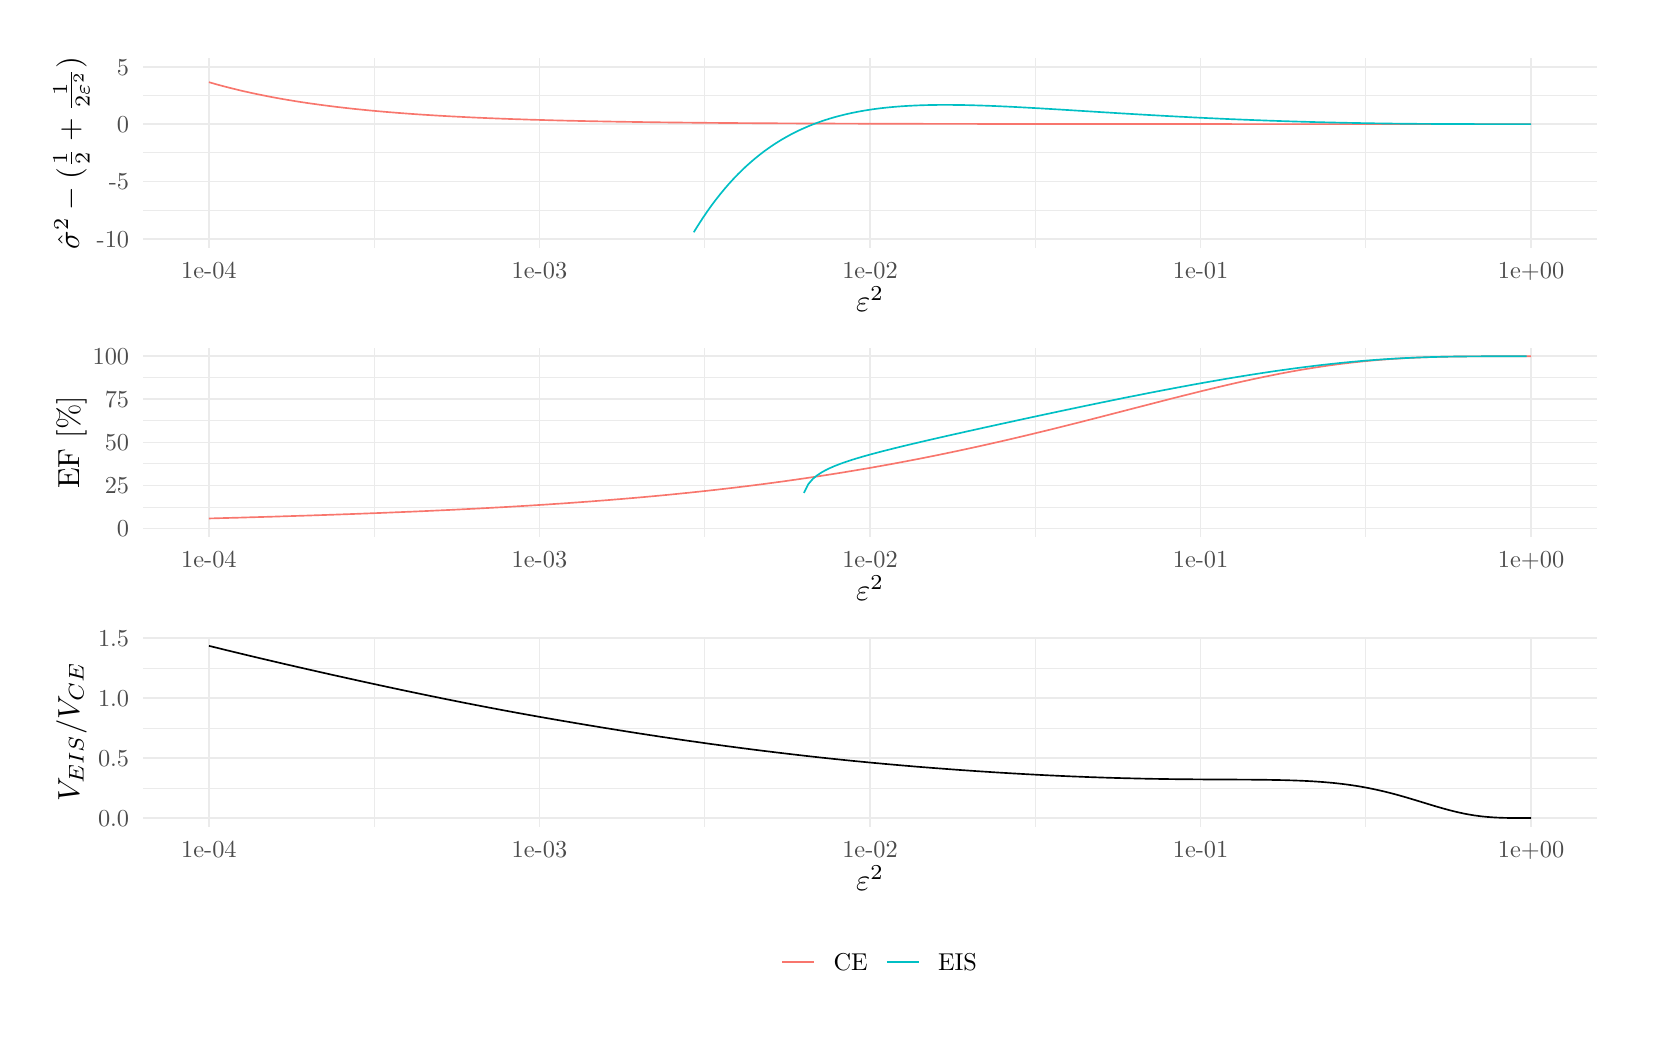
\begin{tikzpicture}[x=1pt,y=1pt]
\definecolor{fillColor}{RGB}{255,255,255}
\path[use as bounding box,fill=fillColor,fill opacity=0.00] (0,0) rectangle (578.16,361.35);
\begin{scope}
\path[clip] ( 41.61,281.90) rectangle (567.16,350.35);
\definecolor{drawColor}{gray}{0.92}

\path[draw=drawColor,line width= 0.3pt,line join=round] ( 41.61,295.39) --
	(567.16,295.39);

\path[draw=drawColor,line width= 0.3pt,line join=round] ( 41.61,316.13) --
	(567.16,316.13);

\path[draw=drawColor,line width= 0.3pt,line join=round] ( 41.61,336.87) --
	(567.16,336.87);

\path[draw=drawColor,line width= 0.3pt,line join=round] (125.22,281.90) --
	(125.22,350.35);

\path[draw=drawColor,line width= 0.3pt,line join=round] (244.66,281.90) --
	(244.66,350.35);

\path[draw=drawColor,line width= 0.3pt,line join=round] (364.11,281.90) --
	(364.11,350.35);

\path[draw=drawColor,line width= 0.3pt,line join=round] (483.55,281.90) --
	(483.55,350.35);

\path[draw=drawColor,line width= 0.6pt,line join=round] ( 41.61,285.02) --
	(567.16,285.02);

\path[draw=drawColor,line width= 0.6pt,line join=round] ( 41.61,305.76) --
	(567.16,305.76);

\path[draw=drawColor,line width= 0.6pt,line join=round] ( 41.61,326.50) --
	(567.16,326.50);

\path[draw=drawColor,line width= 0.6pt,line join=round] ( 41.61,347.24) --
	(567.16,347.24);

\path[draw=drawColor,line width= 0.6pt,line join=round] ( 65.50,281.90) --
	( 65.50,350.35);

\path[draw=drawColor,line width= 0.6pt,line join=round] (184.94,281.90) --
	(184.94,350.35);

\path[draw=drawColor,line width= 0.6pt,line join=round] (304.39,281.90) --
	(304.39,350.35);

\path[draw=drawColor,line width= 0.6pt,line join=round] (423.83,281.90) --
	(423.83,350.35);

\path[draw=drawColor,line width= 0.6pt,line join=round] (543.27,281.90) --
	(543.27,350.35);
\definecolor{drawColor}{RGB}{248,118,109}

\path[draw=drawColor,line width= 0.6pt,line join=round] ( 65.50,341.65) --
	( 67.09,341.19) --
	( 68.68,340.74) --
	( 70.28,340.31) --
	( 71.87,339.90) --
	( 73.46,339.49) --
	( 75.06,339.10) --
	( 76.65,338.71) --
	( 78.24,338.34) --
	( 79.83,337.99) --
	( 81.43,337.64) --
	( 83.02,337.30) --
	( 84.61,336.98) --
	( 86.20,336.66) --
	( 87.80,336.35) --
	( 89.39,336.05) --
	( 90.98,335.76) --
	( 92.57,335.48) --
	( 94.17,335.21) --
	( 95.76,334.95) --
	( 97.35,334.69) --
	( 98.94,334.44) --
	(100.54,334.20) --
	(102.13,333.97) --
	(103.72,333.75) --
	(105.31,333.53) --
	(106.91,333.31) --
	(108.50,333.11) --
	(110.09,332.91) --
	(111.68,332.71) --
	(113.28,332.53) --
	(114.87,332.34) --
	(116.46,332.17) --
	(118.05,331.99) --
	(119.65,331.83) --
	(121.24,331.67) --
	(122.83,331.51) --
	(124.42,331.36) --
	(126.02,331.21) --
	(127.61,331.07) --
	(129.20,330.93) --
	(130.80,330.80) --
	(132.39,330.67) --
	(133.98,330.54) --
	(135.57,330.42) --
	(137.17,330.30) --
	(138.76,330.18) --
	(140.35,330.07) --
	(141.94,329.96) --
	(143.54,329.86) --
	(145.13,329.76) --
	(146.72,329.66) --
	(148.31,329.56) --
	(149.91,329.47) --
	(151.50,329.38) --
	(153.09,329.29) --
	(154.68,329.21) --
	(156.28,329.13) --
	(157.87,329.05) --
	(159.46,328.97) --
	(161.05,328.89) --
	(162.65,328.82) --
	(164.24,328.75) --
	(165.83,328.68) --
	(167.42,328.62) --
	(169.02,328.55) --
	(170.61,328.49) --
	(172.20,328.43) --
	(173.79,328.37) --
	(175.39,328.31) --
	(176.98,328.26) --
	(178.57,328.21) --
	(180.16,328.15) --
	(181.76,328.10) --
	(183.35,328.06) --
	(184.94,328.01) --
	(186.54,327.96) --
	(188.13,327.92) --
	(189.72,327.87) --
	(191.31,327.83) --
	(192.91,327.79) --
	(194.50,327.75) --
	(196.09,327.71) --
	(197.68,327.68) --
	(199.28,327.64) --
	(200.87,327.61) --
	(202.46,327.57) --
	(204.05,327.54) --
	(205.65,327.51) --
	(207.24,327.48) --
	(208.83,327.45) --
	(210.42,327.42) --
	(212.02,327.39) --
	(213.61,327.36) --
	(215.20,327.34) --
	(216.79,327.31) --
	(218.39,327.29) --
	(219.98,327.26) --
	(221.57,327.24) --
	(223.16,327.22) --
	(224.76,327.20) --
	(226.35,327.17) --
	(227.94,327.15) --
	(229.53,327.13) --
	(231.13,327.11) --
	(232.72,327.10) --
	(234.31,327.08) --
	(235.90,327.06) --
	(237.50,327.04) --
	(239.09,327.03) --
	(240.68,327.01) --
	(242.28,326.99) --
	(243.87,326.98) --
	(245.46,326.96) --
	(247.05,326.95) --
	(248.65,326.94) --
	(250.24,326.92) --
	(251.83,326.91) --
	(253.42,326.90) --
	(255.02,326.89) --
	(256.61,326.87) --
	(258.20,326.86) --
	(259.79,326.85) --
	(261.39,326.84) --
	(262.98,326.83) --
	(264.57,326.82) --
	(266.16,326.81) --
	(267.76,326.80) --
	(269.35,326.79) --
	(270.94,326.78) --
	(272.53,326.77) --
	(274.13,326.76) --
	(275.72,326.76) --
	(277.31,326.75) --
	(278.90,326.74) --
	(280.50,326.73) --
	(282.09,326.73) --
	(283.68,326.72) --
	(285.27,326.71) --
	(286.87,326.71) --
	(288.46,326.70) --
	(290.05,326.69) --
	(291.65,326.69) --
	(293.24,326.68) --
	(294.83,326.67) --
	(296.42,326.67) --
	(298.02,326.66) --
	(299.61,326.66) --
	(301.20,326.65) --
	(302.79,326.65) --
	(304.39,326.64) --
	(305.98,326.64) --
	(307.57,326.64) --
	(309.16,326.63) --
	(310.76,326.63) --
	(312.35,326.62) --
	(313.94,326.62) --
	(315.53,326.62) --
	(317.13,326.61) --
	(318.72,326.61) --
	(320.31,326.60) --
	(321.90,326.60) --
	(323.50,326.60) --
	(325.09,326.59) --
	(326.68,326.59) --
	(328.27,326.59) --
	(329.87,326.59) --
	(331.46,326.58) --
	(333.05,326.58) --
	(334.64,326.58) --
	(336.24,326.57) --
	(337.83,326.57) --
	(339.42,326.57) --
	(341.01,326.57) --
	(342.61,326.57) --
	(344.20,326.56) --
	(345.79,326.56) --
	(347.39,326.56) --
	(348.98,326.56) --
	(350.57,326.55) --
	(352.16,326.55) --
	(353.76,326.55) --
	(355.35,326.55) --
	(356.94,326.55) --
	(358.53,326.55) --
	(360.13,326.54) --
	(361.72,326.54) --
	(363.31,326.54) --
	(364.90,326.54) --
	(366.50,326.54) --
	(368.09,326.54) --
	(369.68,326.54) --
	(371.27,326.53) --
	(372.87,326.53) --
	(374.46,326.53) --
	(376.05,326.53) --
	(377.64,326.53) --
	(379.24,326.53) --
	(380.83,326.53) --
	(382.42,326.53) --
	(384.01,326.53) --
	(385.61,326.52) --
	(387.20,326.52) --
	(388.79,326.52) --
	(390.38,326.52) --
	(391.98,326.52) --
	(393.57,326.52) --
	(395.16,326.52) --
	(396.75,326.52) --
	(398.35,326.52) --
	(399.94,326.52) --
	(401.53,326.52) --
	(403.13,326.52) --
	(404.72,326.51) --
	(406.31,326.51) --
	(407.90,326.51) --
	(409.50,326.51) --
	(411.09,326.51) --
	(412.68,326.51) --
	(414.27,326.51) --
	(415.87,326.51) --
	(417.46,326.51) --
	(419.05,326.51) --
	(420.64,326.51) --
	(422.24,326.51) --
	(423.83,326.51) --
	(425.42,326.51) --
	(427.01,326.51) --
	(428.61,326.51) --
	(430.20,326.51) --
	(431.79,326.51) --
	(433.38,326.51) --
	(434.98,326.51) --
	(436.57,326.50) --
	(438.16,326.50) --
	(439.75,326.50) --
	(441.35,326.50) --
	(442.94,326.50) --
	(444.53,326.50) --
	(446.12,326.50) --
	(447.72,326.50) --
	(449.31,326.50) --
	(450.90,326.50) --
	(452.49,326.50) --
	(454.09,326.50) --
	(455.68,326.50) --
	(457.27,326.50) --
	(458.87,326.50) --
	(460.46,326.50) --
	(462.05,326.50) --
	(463.64,326.50) --
	(465.24,326.50) --
	(466.83,326.50) --
	(468.42,326.50) --
	(470.01,326.50) --
	(471.61,326.50) --
	(473.20,326.50) --
	(474.79,326.50) --
	(476.38,326.50) --
	(477.98,326.50) --
	(479.57,326.50) --
	(481.16,326.50) --
	(482.75,326.50) --
	(484.35,326.50) --
	(485.94,326.50) --
	(487.53,326.50) --
	(489.12,326.50) --
	(490.72,326.50) --
	(492.31,326.50) --
	(493.90,326.50) --
	(495.49,326.50) --
	(497.09,326.50) --
	(498.68,326.50) --
	(500.27,326.50) --
	(501.86,326.50) --
	(503.46,326.50) --
	(505.05,326.50) --
	(506.64,326.50) --
	(508.23,326.50) --
	(509.83,326.50) --
	(511.42,326.50) --
	(513.01,326.50) --
	(514.61,326.50) --
	(516.20,326.50) --
	(517.79,326.50) --
	(519.38,326.50) --
	(520.98,326.50) --
	(522.57,326.50) --
	(524.16,326.49) --
	(525.75,326.49) --
	(527.35,326.49) --
	(528.94,326.49) --
	(530.53,326.49) --
	(532.12,326.49) --
	(533.72,326.49) --
	(535.31,326.49) --
	(536.90,326.49) --
	(538.49,326.49) --
	(540.09,326.49) --
	(541.68,326.49) --
	(543.27,326.49);
\definecolor{drawColor}{RGB}{0,191,196}

\path[draw=drawColor,line width= 0.6pt,line join=round] (240.68,287.41) --
	(242.28,289.98) --
	(243.87,292.44) --
	(245.46,294.79) --
	(247.05,297.02) --
	(248.65,299.15) --
	(250.24,301.17) --
	(251.83,303.10) --
	(253.42,304.94) --
	(255.02,306.69) --
	(256.61,308.35) --
	(258.20,309.92) --
	(259.79,311.42) --
	(261.39,312.84) --
	(262.98,314.19) --
	(264.57,315.47) --
	(266.16,316.69) --
	(267.76,317.84) --
	(269.35,318.93) --
	(270.94,319.96) --
	(272.53,320.93) --
	(274.13,321.85) --
	(275.72,322.72) --
	(277.31,323.54) --
	(278.90,324.31) --
	(280.50,325.03) --
	(282.09,325.72) --
	(283.68,326.36) --
	(285.27,326.96) --
	(286.87,327.53) --
	(288.46,328.06) --
	(290.05,328.56) --
	(291.65,329.02) --
	(293.24,329.45) --
	(294.83,329.85) --
	(296.42,330.23) --
	(298.02,330.57) --
	(299.61,330.89) --
	(301.20,331.19) --
	(302.79,331.46) --
	(304.39,331.71) --
	(305.98,331.94) --
	(307.57,332.15) --
	(309.16,332.34) --
	(310.76,332.51) --
	(312.35,332.66) --
	(313.94,332.80) --
	(315.53,332.92) --
	(317.13,333.03) --
	(318.72,333.12) --
	(320.31,333.20) --
	(321.90,333.27) --
	(323.50,333.33) --
	(325.09,333.37) --
	(326.68,333.40) --
	(328.27,333.43) --
	(329.87,333.44) --
	(331.46,333.45) --
	(333.05,333.44) --
	(334.64,333.43) --
	(336.24,333.41) --
	(337.83,333.39) --
	(339.42,333.36) --
	(341.01,333.32) --
	(342.61,333.27) --
	(344.20,333.22) --
	(345.79,333.17) --
	(347.39,333.11) --
	(348.98,333.05) --
	(350.57,332.98) --
	(352.16,332.91) --
	(353.76,332.84) --
	(355.35,332.76) --
	(356.94,332.68) --
	(358.53,332.59) --
	(360.13,332.51) --
	(361.72,332.42) --
	(363.31,332.33) --
	(364.90,332.24) --
	(366.50,332.15) --
	(368.09,332.05) --
	(369.68,331.96) --
	(371.27,331.86) --
	(372.87,331.77) --
	(374.46,331.67) --
	(376.05,331.57) --
	(377.64,331.47) --
	(379.24,331.37) --
	(380.83,331.27) --
	(382.42,331.17) --
	(384.01,331.07) --
	(385.61,330.97) --
	(387.20,330.87) --
	(388.79,330.77) --
	(390.38,330.68) --
	(391.98,330.58) --
	(393.57,330.48) --
	(395.16,330.38) --
	(396.75,330.29) --
	(398.35,330.19) --
	(399.94,330.10) --
	(401.53,330.00) --
	(403.13,329.91) --
	(404.72,329.82) --
	(406.31,329.73) --
	(407.90,329.64) --
	(409.50,329.55) --
	(411.09,329.46) --
	(412.68,329.37) --
	(414.27,329.29) --
	(415.87,329.20) --
	(417.46,329.12) --
	(419.05,329.04) --
	(420.64,328.95) --
	(422.24,328.87) --
	(423.83,328.80) --
	(425.42,328.72) --
	(427.01,328.64) --
	(428.61,328.57) --
	(430.20,328.50) --
	(431.79,328.42) --
	(433.38,328.35) --
	(434.98,328.28) --
	(436.57,328.22) --
	(438.16,328.15) --
	(439.75,328.09) --
	(441.35,328.02) --
	(442.94,327.96) --
	(444.53,327.90) --
	(446.12,327.84) --
	(447.72,327.78) --
	(449.31,327.72) --
	(450.90,327.67) --
	(452.49,327.61) --
	(454.09,327.56) --
	(455.68,327.51) --
	(457.27,327.46) --
	(458.87,327.41) --
	(460.46,327.37) --
	(462.05,327.32) --
	(463.64,327.28) --
	(465.24,327.23) --
	(466.83,327.19) --
	(468.42,327.15) --
	(470.01,327.11) --
	(471.61,327.07) --
	(473.20,327.04) --
	(474.79,327.00) --
	(476.38,326.97) --
	(477.98,326.94) --
	(479.57,326.91) --
	(481.16,326.88) --
	(482.75,326.85) --
	(484.35,326.82) --
	(485.94,326.79) --
	(487.53,326.77) --
	(489.12,326.75) --
	(490.72,326.72) --
	(492.31,326.70) --
	(493.90,326.68) --
	(495.49,326.66) --
	(497.09,326.65) --
	(498.68,326.63) --
	(500.27,326.62) --
	(501.86,326.60) --
	(503.46,326.59) --
	(505.05,326.58) --
	(506.64,326.57) --
	(508.23,326.56) --
	(509.83,326.55) --
	(511.42,326.54) --
	(513.01,326.53) --
	(514.61,326.53) --
	(516.20,326.52) --
	(517.79,326.52) --
	(519.38,326.51) --
	(520.98,326.51) --
	(522.57,326.51) --
	(524.16,326.50) --
	(525.75,326.50) --
	(527.35,326.50) --
	(528.94,326.50) --
	(530.53,326.50) --
	(532.12,326.50) --
	(533.72,326.50) --
	(535.31,326.50) --
	(536.90,326.50) --
	(538.49,326.50) --
	(540.09,326.50) --
	(541.68,326.50) --
	(543.27,326.50);
\end{scope}
\begin{scope}
\path[clip] (  0.00,  0.00) rectangle (578.16,361.35);
\definecolor{drawColor}{gray}{0.30}

\node[text=drawColor,anchor=base east,inner sep=0pt, outer sep=0pt, scale=  0.88] at ( 36.66,281.98) {-10};

\node[text=drawColor,anchor=base east,inner sep=0pt, outer sep=0pt, scale=  0.88] at ( 36.66,302.73) {-5};

\node[text=drawColor,anchor=base east,inner sep=0pt, outer sep=0pt, scale=  0.88] at ( 36.66,323.47) {0};

\node[text=drawColor,anchor=base east,inner sep=0pt, outer sep=0pt, scale=  0.88] at ( 36.66,344.21) {5};
\end{scope}
\begin{scope}
\path[clip] (  0.00,  0.00) rectangle (578.16,361.35);
\definecolor{drawColor}{gray}{0.30}

\node[text=drawColor,anchor=base,inner sep=0pt, outer sep=0pt, scale=  0.88] at ( 65.50,270.89) {1e-04};

\node[text=drawColor,anchor=base,inner sep=0pt, outer sep=0pt, scale=  0.88] at (184.94,270.89) {1e-03};

\node[text=drawColor,anchor=base,inner sep=0pt, outer sep=0pt, scale=  0.88] at (304.39,270.89) {1e-02};

\node[text=drawColor,anchor=base,inner sep=0pt, outer sep=0pt, scale=  0.88] at (423.83,270.89) {1e-01};

\node[text=drawColor,anchor=base,inner sep=0pt, outer sep=0pt, scale=  0.88] at (543.27,270.89) {1e+00};
\end{scope}
\begin{scope}
\path[clip] (  0.00,  0.00) rectangle (578.16,361.35);
\definecolor{drawColor}{RGB}{0,0,0}

\node[text=drawColor,anchor=base,inner sep=0pt, outer sep=0pt, scale=  1.10] at (304.39,258.86) {$\varepsilon^2$};
\end{scope}
\begin{scope}
\path[clip] (  0.00,  0.00) rectangle (578.16,361.35);
\definecolor{drawColor}{RGB}{0,0,0}

\node[text=drawColor,rotate= 90.00,anchor=base,inner sep=0pt, outer sep=0pt, scale=  1.10] at ( 18.58,316.13) {$\hat \sigma^2 - (\frac 1 2 + \frac 1 {2\varepsilon^2})$};
\end{scope}
\begin{scope}
\path[clip] ( 41.61,177.27) rectangle (567.16,245.72);
\definecolor{drawColor}{gray}{0.92}

\path[draw=drawColor,line width= 0.3pt,line join=round] ( 41.61,188.16) --
	(567.16,188.16);

\path[draw=drawColor,line width= 0.3pt,line join=round] ( 41.61,203.72) --
	(567.16,203.72);

\path[draw=drawColor,line width= 0.3pt,line join=round] ( 41.61,219.27) --
	(567.16,219.27);

\path[draw=drawColor,line width= 0.3pt,line join=round] ( 41.61,234.83) --
	(567.16,234.83);

\path[draw=drawColor,line width= 0.3pt,line join=round] (125.22,177.27) --
	(125.22,245.72);

\path[draw=drawColor,line width= 0.3pt,line join=round] (244.66,177.27) --
	(244.66,245.72);

\path[draw=drawColor,line width= 0.3pt,line join=round] (364.11,177.27) --
	(364.11,245.72);

\path[draw=drawColor,line width= 0.3pt,line join=round] (483.55,177.27) --
	(483.55,245.72);

\path[draw=drawColor,line width= 0.6pt,line join=round] ( 41.61,180.38) --
	(567.16,180.38);

\path[draw=drawColor,line width= 0.6pt,line join=round] ( 41.61,195.94) --
	(567.16,195.94);

\path[draw=drawColor,line width= 0.6pt,line join=round] ( 41.61,211.49) --
	(567.16,211.49);

\path[draw=drawColor,line width= 0.6pt,line join=round] ( 41.61,227.05) --
	(567.16,227.05);

\path[draw=drawColor,line width= 0.6pt,line join=round] ( 41.61,242.61) --
	(567.16,242.61);

\path[draw=drawColor,line width= 0.6pt,line join=round] ( 65.50,177.27) --
	( 65.50,245.72);

\path[draw=drawColor,line width= 0.6pt,line join=round] (184.94,177.27) --
	(184.94,245.72);

\path[draw=drawColor,line width= 0.6pt,line join=round] (304.39,177.27) --
	(304.39,245.72);

\path[draw=drawColor,line width= 0.6pt,line join=round] (423.83,177.27) --
	(423.83,245.72);

\path[draw=drawColor,line width= 0.6pt,line join=round] (543.27,177.27) --
	(543.27,245.72);
\definecolor{drawColor}{RGB}{248,118,109}

\path[draw=drawColor,line width= 0.6pt,line join=round] ( 65.50,184.00) --
	( 67.09,184.04) --
	( 68.68,184.09) --
	( 70.28,184.13) --
	( 71.87,184.17) --
	( 73.46,184.22) --
	( 75.06,184.26) --
	( 76.65,184.30) --
	( 78.24,184.35) --
	( 79.83,184.40) --
	( 81.43,184.44) --
	( 83.02,184.49) --
	( 84.61,184.54) --
	( 86.20,184.58) --
	( 87.80,184.63) --
	( 89.39,184.68) --
	( 90.98,184.73) --
	( 92.57,184.78) --
	( 94.17,184.83) --
	( 95.76,184.88) --
	( 97.35,184.93) --
	( 98.94,184.98) --
	(100.54,185.03) --
	(102.13,185.08) --
	(103.72,185.14) --
	(105.31,185.19) --
	(106.91,185.24) --
	(108.50,185.30) --
	(110.09,185.35) --
	(111.68,185.41) --
	(113.28,185.47) --
	(114.87,185.52) --
	(116.46,185.58) --
	(118.05,185.64) --
	(119.65,185.70) --
	(121.24,185.76) --
	(122.83,185.82) --
	(124.42,185.88) --
	(126.02,185.94) --
	(127.61,186.00) --
	(129.20,186.07) --
	(130.80,186.13) --
	(132.39,186.20) --
	(133.98,186.26) --
	(135.57,186.33) --
	(137.17,186.40) --
	(138.76,186.46) --
	(140.35,186.53) --
	(141.94,186.60) --
	(143.54,186.67) --
	(145.13,186.74) --
	(146.72,186.82) --
	(148.31,186.89) --
	(149.91,186.96) --
	(151.50,187.04) --
	(153.09,187.11) --
	(154.68,187.19) --
	(156.28,187.27) --
	(157.87,187.35) --
	(159.46,187.43) --
	(161.05,187.51) --
	(162.65,187.59) --
	(164.24,187.68) --
	(165.83,187.76) --
	(167.42,187.85) --
	(169.02,187.94) --
	(170.61,188.02) --
	(172.20,188.11) --
	(173.79,188.20) --
	(175.39,188.30) --
	(176.98,188.39) --
	(178.57,188.49) --
	(180.16,188.58) --
	(181.76,188.68) --
	(183.35,188.78) --
	(184.94,188.88) --
	(186.54,188.98) --
	(188.13,189.08) --
	(189.72,189.19) --
	(191.31,189.30) --
	(192.91,189.40) --
	(194.50,189.51) --
	(196.09,189.62) --
	(197.68,189.74) --
	(199.28,189.85) --
	(200.87,189.97) --
	(202.46,190.08) --
	(204.05,190.20) --
	(205.65,190.33) --
	(207.24,190.45) --
	(208.83,190.57) --
	(210.42,190.70) --
	(212.02,190.83) --
	(213.61,190.96) --
	(215.20,191.09) --
	(216.79,191.23) --
	(218.39,191.36) --
	(219.98,191.50) --
	(221.57,191.64) --
	(223.16,191.78) --
	(224.76,191.93) --
	(226.35,192.07) --
	(227.94,192.22) --
	(229.53,192.37) --
	(231.13,192.52) --
	(232.72,192.68) --
	(234.31,192.84) --
	(235.90,193.00) --
	(237.50,193.16) --
	(239.09,193.32) --
	(240.68,193.49) --
	(242.28,193.66) --
	(243.87,193.83) --
	(245.46,194.00) --
	(247.05,194.18) --
	(248.65,194.35) --
	(250.24,194.54) --
	(251.83,194.72) --
	(253.42,194.90) --
	(255.02,195.09) --
	(256.61,195.28) --
	(258.20,195.48) --
	(259.79,195.67) --
	(261.39,195.87) --
	(262.98,196.07) --
	(264.57,196.27) --
	(266.16,196.48) --
	(267.76,196.69) --
	(269.35,196.90) --
	(270.94,197.12) --
	(272.53,197.33) --
	(274.13,197.55) --
	(275.72,197.78) --
	(277.31,198.00) --
	(278.90,198.23) --
	(280.50,198.46) --
	(282.09,198.70) --
	(283.68,198.93) --
	(285.27,199.17) --
	(286.87,199.42) --
	(288.46,199.66) --
	(290.05,199.91) --
	(291.65,200.16) --
	(293.24,200.42) --
	(294.83,200.67) --
	(296.42,200.94) --
	(298.02,201.20) --
	(299.61,201.47) --
	(301.20,201.74) --
	(302.79,202.01) --
	(304.39,202.28) --
	(305.98,202.56) --
	(307.57,202.85) --
	(309.16,203.13) --
	(310.76,203.42) --
	(312.35,203.71) --
	(313.94,204.00) --
	(315.53,204.30) --
	(317.13,204.60) --
	(318.72,204.91) --
	(320.31,205.21) --
	(321.90,205.52) --
	(323.50,205.84) --
	(325.09,206.15) --
	(326.68,206.47) --
	(328.27,206.79) --
	(329.87,207.12) --
	(331.46,207.45) --
	(333.05,207.78) --
	(334.64,208.11) --
	(336.24,208.45) --
	(337.83,208.79) --
	(339.42,209.13) --
	(341.01,209.48) --
	(342.61,209.82) --
	(344.20,210.18) --
	(345.79,210.53) --
	(347.39,210.89) --
	(348.98,211.25) --
	(350.57,211.61) --
	(352.16,211.97) --
	(353.76,212.34) --
	(355.35,212.71) --
	(356.94,213.09) --
	(358.53,213.46) --
	(360.13,213.84) --
	(361.72,214.22) --
	(363.31,214.60) --
	(364.90,214.99) --
	(366.50,215.37) --
	(368.09,215.76) --
	(369.68,216.15) --
	(371.27,216.55) --
	(372.87,216.94) --
	(374.46,217.34) --
	(376.05,217.74) --
	(377.64,218.14) --
	(379.24,218.54) --
	(380.83,218.94) --
	(382.42,219.35) --
	(384.01,219.75) --
	(385.61,220.16) --
	(387.20,220.57) --
	(388.79,220.98) --
	(390.38,221.39) --
	(391.98,221.80) --
	(393.57,222.21) --
	(395.16,222.62) --
	(396.75,223.03) --
	(398.35,223.45) --
	(399.94,223.86) --
	(401.53,224.27) --
	(403.13,224.68) --
	(404.72,225.09) --
	(406.31,225.50) --
	(407.90,225.91) --
	(409.50,226.32) --
	(411.09,226.73) --
	(412.68,227.14) --
	(414.27,227.54) --
	(415.87,227.94) --
	(417.46,228.35) --
	(419.05,228.74) --
	(420.64,229.14) --
	(422.24,229.54) --
	(423.83,229.93) --
	(425.42,230.32) --
	(427.01,230.70) --
	(428.61,231.09) --
	(430.20,231.47) --
	(431.79,231.84) --
	(433.38,232.22) --
	(434.98,232.58) --
	(436.57,232.95) --
	(438.16,233.31) --
	(439.75,233.66) --
	(441.35,234.01) --
	(442.94,234.36) --
	(444.53,234.70) --
	(446.12,235.03) --
	(447.72,235.36) --
	(449.31,235.68) --
	(450.90,236.00) --
	(452.49,236.31) --
	(454.09,236.61) --
	(455.68,236.91) --
	(457.27,237.20) --
	(458.87,237.48) --
	(460.46,237.76) --
	(462.05,238.02) --
	(463.64,238.28) --
	(465.24,238.54) --
	(466.83,238.78) --
	(468.42,239.02) --
	(470.01,239.25) --
	(471.61,239.47) --
	(473.20,239.68) --
	(474.79,239.89) --
	(476.38,240.08) --
	(477.98,240.27) --
	(479.57,240.45) --
	(481.16,240.62) --
	(482.75,240.78) --
	(484.35,240.94) --
	(485.94,241.08) --
	(487.53,241.22) --
	(489.12,241.35) --
	(490.72,241.47) --
	(492.31,241.59) --
	(493.90,241.70) --
	(495.49,241.79) --
	(497.09,241.89) --
	(498.68,241.97) --
	(500.27,242.05) --
	(501.86,242.12) --
	(503.46,242.19) --
	(505.05,242.24) --
	(506.64,242.30) --
	(508.23,242.34) --
	(509.83,242.39) --
	(511.42,242.42) --
	(513.01,242.46) --
	(514.61,242.48) --
	(516.20,242.51) --
	(517.79,242.53) --
	(519.38,242.55) --
	(520.98,242.56) --
	(522.57,242.57) --
	(524.16,242.58) --
	(525.75,242.59) --
	(527.35,242.59) --
	(528.94,242.60) --
	(530.53,242.60) --
	(532.12,242.60) --
	(533.72,242.61) --
	(535.31,242.61) --
	(536.90,242.61) --
	(538.49,242.61) --
	(540.09,242.61) --
	(541.68,242.61) --
	(543.27,242.61);
\definecolor{drawColor}{RGB}{0,191,196}

\path[draw=drawColor,line width= 0.6pt,line join=round] (280.50,193.24) --
	(282.09,196.41) --
	(283.68,198.26) --
	(285.27,199.59) --
	(286.87,200.64) --
	(288.46,201.52) --
	(290.05,202.28) --
	(291.65,202.97) --
	(293.24,203.59) --
	(294.83,204.17) --
	(296.42,204.72) --
	(298.02,205.23) --
	(299.61,205.72) --
	(301.20,206.19) --
	(302.79,206.65) --
	(304.39,207.09) --
	(305.98,207.52) --
	(307.57,207.94) --
	(309.16,208.36) --
	(310.76,208.76) --
	(312.35,209.16) --
	(313.94,209.56) --
	(315.53,209.94) --
	(317.13,210.33) --
	(318.72,210.71) --
	(320.31,211.09) --
	(321.90,211.46) --
	(323.50,211.83) --
	(325.09,212.20) --
	(326.68,212.57) --
	(328.27,212.93) --
	(329.87,213.30) --
	(331.46,213.66) --
	(333.05,214.02) --
	(334.64,214.38) --
	(336.24,214.73) --
	(337.83,215.09) --
	(339.42,215.45) --
	(341.01,215.80) --
	(342.61,216.15) --
	(344.20,216.51) --
	(345.79,216.86) --
	(347.39,217.21) --
	(348.98,217.56) --
	(350.57,217.91) --
	(352.16,218.26) --
	(353.76,218.60) --
	(355.35,218.95) --
	(356.94,219.30) --
	(358.53,219.64) --
	(360.13,219.99) --
	(361.72,220.33) --
	(363.31,220.68) --
	(364.90,221.02) --
	(366.50,221.36) --
	(368.09,221.70) --
	(369.68,222.04) --
	(371.27,222.38) --
	(372.87,222.72) --
	(374.46,223.06) --
	(376.05,223.39) --
	(377.64,223.73) --
	(379.24,224.06) --
	(380.83,224.40) --
	(382.42,224.73) --
	(384.01,225.06) --
	(385.61,225.39) --
	(387.20,225.72) --
	(388.79,226.05) --
	(390.38,226.37) --
	(391.98,226.70) --
	(393.57,227.02) --
	(395.16,227.35) --
	(396.75,227.67) --
	(398.35,227.99) --
	(399.94,228.30) --
	(401.53,228.62) --
	(403.13,228.93) --
	(404.72,229.25) --
	(406.31,229.56) --
	(407.90,229.87) --
	(409.50,230.17) --
	(411.09,230.48) --
	(412.68,230.78) --
	(414.27,231.08) --
	(415.87,231.38) --
	(417.46,231.68) --
	(419.05,231.97) --
	(420.64,232.27) --
	(422.24,232.56) --
	(423.83,232.84) --
	(425.42,233.13) --
	(427.01,233.41) --
	(428.61,233.69) --
	(430.20,233.96) --
	(431.79,234.24) --
	(433.38,234.51) --
	(434.98,234.78) --
	(436.57,235.04) --
	(438.16,235.30) --
	(439.75,235.56) --
	(441.35,235.82) --
	(442.94,236.07) --
	(444.53,236.31) --
	(446.12,236.56) --
	(447.72,236.80) --
	(449.31,237.04) --
	(450.90,237.27) --
	(452.49,237.50) --
	(454.09,237.72) --
	(455.68,237.94) --
	(457.27,238.16) --
	(458.87,238.37) --
	(460.46,238.58) --
	(462.05,238.78) --
	(463.64,238.98) --
	(465.24,239.18) --
	(466.83,239.37) --
	(468.42,239.55) --
	(470.01,239.73) --
	(471.61,239.90) --
	(473.20,240.07) --
	(474.79,240.24) --
	(476.38,240.39) --
	(477.98,240.55) --
	(479.57,240.69) --
	(481.16,240.83) --
	(482.75,240.97) --
	(484.35,241.10) --
	(485.94,241.22) --
	(487.53,241.34) --
	(489.12,241.45) --
	(490.72,241.56) --
	(492.31,241.66) --
	(493.90,241.76) --
	(495.49,241.84) --
	(497.09,241.93) --
	(498.68,242.00) --
	(500.27,242.07) --
	(501.86,242.14) --
	(503.46,242.20) --
	(505.05,242.26) --
	(506.64,242.31) --
	(508.23,242.35) --
	(509.83,242.39) --
	(511.42,242.43) --
	(513.01,242.46) --
	(514.61,242.49) --
	(516.20,242.51) --
	(517.79,242.53) --
	(519.38,242.55) --
	(520.98,242.56) --
	(522.57,242.57) --
	(524.16,242.58) --
	(525.75,242.59) --
	(527.35,242.59) --
	(528.94,242.60) --
	(530.53,242.60) --
	(532.12,242.60) --
	(533.72,242.61) --
	(535.31,242.61) --
	(536.90,242.61) --
	(538.49,242.61) --
	(540.09,242.61) --
	(541.68,242.61);
\end{scope}
\begin{scope}
\path[clip] (  0.00,  0.00) rectangle (578.16,361.35);
\definecolor{drawColor}{gray}{0.30}

\node[text=drawColor,anchor=base east,inner sep=0pt, outer sep=0pt, scale=  0.88] at ( 36.66,177.35) {0};

\node[text=drawColor,anchor=base east,inner sep=0pt, outer sep=0pt, scale=  0.88] at ( 36.66,192.91) {25};

\node[text=drawColor,anchor=base east,inner sep=0pt, outer sep=0pt, scale=  0.88] at ( 36.66,208.46) {50};

\node[text=drawColor,anchor=base east,inner sep=0pt, outer sep=0pt, scale=  0.88] at ( 36.66,224.02) {75};

\node[text=drawColor,anchor=base east,inner sep=0pt, outer sep=0pt, scale=  0.88] at ( 36.66,239.58) {100};
\end{scope}
\begin{scope}
\path[clip] (  0.00,  0.00) rectangle (578.16,361.35);
\definecolor{drawColor}{gray}{0.30}

\node[text=drawColor,anchor=base,inner sep=0pt, outer sep=0pt, scale=  0.88] at ( 65.50,166.26) {1e-04};

\node[text=drawColor,anchor=base,inner sep=0pt, outer sep=0pt, scale=  0.88] at (184.94,166.26) {1e-03};

\node[text=drawColor,anchor=base,inner sep=0pt, outer sep=0pt, scale=  0.88] at (304.39,166.26) {1e-02};

\node[text=drawColor,anchor=base,inner sep=0pt, outer sep=0pt, scale=  0.88] at (423.83,166.26) {1e-01};

\node[text=drawColor,anchor=base,inner sep=0pt, outer sep=0pt, scale=  0.88] at (543.27,166.26) {1e+00};
\end{scope}
\begin{scope}
\path[clip] (  0.00,  0.00) rectangle (578.16,361.35);
\definecolor{drawColor}{RGB}{0,0,0}

\node[text=drawColor,anchor=base,inner sep=0pt, outer sep=0pt, scale=  1.10] at (304.39,154.22) {$\varepsilon^2$};
\end{scope}
\begin{scope}
\path[clip] (  0.00,  0.00) rectangle (578.16,361.35);
\definecolor{drawColor}{RGB}{0,0,0}

\node[text=drawColor,rotate= 90.00,anchor=base,inner sep=0pt, outer sep=0pt, scale=  1.10] at ( 18.58,211.49) {EF [\%]};
\end{scope}
\begin{scope}
\path[clip] ( 41.61, 72.64) rectangle (567.16,141.09);
\definecolor{drawColor}{gray}{0.92}

\path[draw=drawColor,line width= 0.3pt,line join=round] ( 41.61, 86.59) --
	(567.16, 86.59);

\path[draw=drawColor,line width= 0.3pt,line join=round] ( 41.61,108.27) --
	(567.16,108.27);

\path[draw=drawColor,line width= 0.3pt,line join=round] ( 41.61,129.94) --
	(567.16,129.94);

\path[draw=drawColor,line width= 0.3pt,line join=round] (125.22, 72.64) --
	(125.22,141.09);

\path[draw=drawColor,line width= 0.3pt,line join=round] (244.66, 72.64) --
	(244.66,141.09);

\path[draw=drawColor,line width= 0.3pt,line join=round] (364.11, 72.64) --
	(364.11,141.09);

\path[draw=drawColor,line width= 0.3pt,line join=round] (483.55, 72.64) --
	(483.55,141.09);

\path[draw=drawColor,line width= 0.6pt,line join=round] ( 41.61, 75.75) --
	(567.16, 75.75);

\path[draw=drawColor,line width= 0.6pt,line join=round] ( 41.61, 97.43) --
	(567.16, 97.43);

\path[draw=drawColor,line width= 0.6pt,line join=round] ( 41.61,119.10) --
	(567.16,119.10);

\path[draw=drawColor,line width= 0.6pt,line join=round] ( 41.61,140.78) --
	(567.16,140.78);

\path[draw=drawColor,line width= 0.6pt,line join=round] ( 65.50, 72.64) --
	( 65.50,141.09);

\path[draw=drawColor,line width= 0.6pt,line join=round] (184.94, 72.64) --
	(184.94,141.09);

\path[draw=drawColor,line width= 0.6pt,line join=round] (304.39, 72.64) --
	(304.39,141.09);

\path[draw=drawColor,line width= 0.6pt,line join=round] (423.83, 72.64) --
	(423.83,141.09);

\path[draw=drawColor,line width= 0.6pt,line join=round] (543.27, 72.64) --
	(543.27,141.09);
\definecolor{drawColor}{RGB}{0,0,0}

\path[draw=drawColor,line width= 0.6pt,line join=round] ( 65.50,137.97) --
	( 67.09,137.58) --
	( 68.68,137.19) --
	( 70.28,136.80) --
	( 71.87,136.40) --
	( 73.46,136.02) --
	( 75.06,135.63) --
	( 76.65,135.25) --
	( 78.24,134.86) --
	( 79.83,134.48) --
	( 81.43,134.10) --
	( 83.02,133.72) --
	( 84.61,133.34) --
	( 86.20,132.97) --
	( 87.80,132.60) --
	( 89.39,132.22) --
	( 90.98,131.85) --
	( 92.57,131.48) --
	( 94.17,131.11) --
	( 95.76,130.75) --
	( 97.35,130.38) --
	( 98.94,130.02) --
	(100.54,129.65) --
	(102.13,129.29) --
	(103.72,128.93) --
	(105.31,128.57) --
	(106.91,128.21) --
	(108.50,127.85) --
	(110.09,127.49) --
	(111.68,127.14) --
	(113.28,126.79) --
	(114.87,126.43) --
	(116.46,126.08) --
	(118.05,125.73) --
	(119.65,125.37) --
	(121.24,125.03) --
	(122.83,124.68) --
	(124.42,124.33) --
	(126.02,123.99) --
	(127.61,123.64) --
	(129.20,123.30) --
	(130.80,122.96) --
	(132.39,122.62) --
	(133.98,122.28) --
	(135.57,121.94) --
	(137.17,121.61) --
	(138.76,121.27) --
	(140.35,120.94) --
	(141.94,120.61) --
	(143.54,120.28) --
	(145.13,119.95) --
	(146.72,119.62) --
	(148.31,119.30) --
	(149.91,118.97) --
	(151.50,118.65) --
	(153.09,118.33) --
	(154.68,118.01) --
	(156.28,117.70) --
	(157.87,117.38) --
	(159.46,117.07) --
	(161.05,116.76) --
	(162.65,116.45) --
	(164.24,116.14) --
	(165.83,115.84) --
	(167.42,115.53) --
	(169.02,115.23) --
	(170.61,114.93) --
	(172.20,114.63) --
	(173.79,114.34) --
	(175.39,114.04) --
	(176.98,113.75) --
	(178.57,113.46) --
	(180.16,113.17) --
	(181.76,112.89) --
	(183.35,112.60) --
	(184.94,112.32) --
	(186.54,112.04) --
	(188.13,111.76) --
	(189.72,111.48) --
	(191.31,111.21) --
	(192.91,110.93) --
	(194.50,110.66) --
	(196.09,110.39) --
	(197.68,110.12) --
	(199.28,109.85) --
	(200.87,109.58) --
	(202.46,109.31) --
	(204.05,109.05) --
	(205.65,108.79) --
	(207.24,108.52) --
	(208.83,108.26) --
	(210.42,108.01) --
	(212.02,107.75) --
	(213.61,107.49) --
	(215.20,107.24) --
	(216.79,106.98) --
	(218.39,106.73) --
	(219.98,106.48) --
	(221.57,106.23) --
	(223.16,105.99) --
	(224.76,105.74) --
	(226.35,105.50) --
	(227.94,105.25) --
	(229.53,105.01) --
	(231.13,104.78) --
	(232.72,104.54) --
	(234.31,104.31) --
	(235.90,104.07) --
	(237.50,103.84) --
	(239.09,103.61) --
	(240.68,103.39) --
	(242.28,103.16) --
	(243.87,102.94) --
	(245.46,102.71) --
	(247.05,102.49) --
	(248.65,102.28) --
	(250.24,102.06) --
	(251.83,101.84) --
	(253.42,101.63) --
	(255.02,101.42) --
	(256.61,101.21) --
	(258.20,101.00) --
	(259.79,100.80) --
	(261.39,100.59) --
	(262.98,100.39) --
	(264.57,100.19) --
	(266.16, 99.99) --
	(267.76, 99.80) --
	(269.35, 99.60) --
	(270.94, 99.41) --
	(272.53, 99.22) --
	(274.13, 99.03) --
	(275.72, 98.84) --
	(277.31, 98.66) --
	(278.90, 98.47) --
	(280.50, 98.29) --
	(282.09, 98.11) --
	(283.68, 97.93) --
	(285.27, 97.76) --
	(286.87, 97.58) --
	(288.46, 97.41) --
	(290.05, 97.24) --
	(291.65, 97.07) --
	(293.24, 96.91) --
	(294.83, 96.74) --
	(296.42, 96.58) --
	(298.02, 96.42) --
	(299.61, 96.26) --
	(301.20, 96.11) --
	(302.79, 95.96) --
	(304.39, 95.80) --
	(305.98, 95.65) --
	(307.57, 95.51) --
	(309.16, 95.36) --
	(310.76, 95.22) --
	(312.35, 95.08) --
	(313.94, 94.94) --
	(315.53, 94.80) --
	(317.13, 94.66) --
	(318.72, 94.53) --
	(320.31, 94.39) --
	(321.90, 94.26) --
	(323.50, 94.13) --
	(325.09, 94.01) --
	(326.68, 93.88) --
	(328.27, 93.76) --
	(329.87, 93.64) --
	(331.46, 93.52) --
	(333.05, 93.40) --
	(334.64, 93.28) --
	(336.24, 93.16) --
	(337.83, 93.05) --
	(339.42, 92.94) --
	(341.01, 92.83) --
	(342.61, 92.72) --
	(344.20, 92.61) --
	(345.79, 92.51) --
	(347.39, 92.41) --
	(348.98, 92.30) --
	(350.57, 92.20) --
	(352.16, 92.10) --
	(353.76, 92.01) --
	(355.35, 91.91) --
	(356.94, 91.82) --
	(358.53, 91.73) --
	(360.13, 91.64) --
	(361.72, 91.55) --
	(363.31, 91.47) --
	(364.90, 91.38) --
	(366.50, 91.30) --
	(368.09, 91.22) --
	(369.68, 91.14) --
	(371.27, 91.07) --
	(372.87, 90.99) --
	(374.46, 90.92) --
	(376.05, 90.85) --
	(377.64, 90.78) --
	(379.24, 90.72) --
	(380.83, 90.66) --
	(382.42, 90.59) --
	(384.01, 90.53) --
	(385.61, 90.48) --
	(387.20, 90.42) --
	(388.79, 90.37) --
	(390.38, 90.32) --
	(391.98, 90.27) --
	(393.57, 90.22) --
	(395.16, 90.18) --
	(396.75, 90.13) --
	(398.35, 90.10) --
	(399.94, 90.06) --
	(401.53, 90.02) --
	(403.13, 89.99) --
	(404.72, 89.95) --
	(406.31, 89.92) --
	(407.90, 89.90) --
	(409.50, 89.87) --
	(411.09, 89.85) --
	(412.68, 89.82) --
	(414.27, 89.80) --
	(415.87, 89.78) --
	(417.46, 89.77) --
	(419.05, 89.75) --
	(420.64, 89.74) --
	(422.24, 89.73) --
	(423.83, 89.71) --
	(425.42, 89.70) --
	(427.01, 89.69) --
	(428.61, 89.69) --
	(430.20, 89.68) --
	(431.79, 89.67) --
	(433.38, 89.66) --
	(434.98, 89.66) --
	(436.57, 89.65) --
	(438.16, 89.64) --
	(439.75, 89.63) --
	(441.35, 89.62) --
	(442.94, 89.61) --
	(444.53, 89.59) --
	(446.12, 89.58) --
	(447.72, 89.56) --
	(449.31, 89.53) --
	(450.90, 89.50) --
	(452.49, 89.47) --
	(454.09, 89.44) --
	(455.68, 89.39) --
	(457.27, 89.34) --
	(458.87, 89.28) --
	(460.46, 89.22) --
	(462.05, 89.14) --
	(463.64, 89.06) --
	(465.24, 88.96) --
	(466.83, 88.85) --
	(468.42, 88.73) --
	(470.01, 88.59) --
	(471.61, 88.45) --
	(473.20, 88.28) --
	(474.79, 88.10) --
	(476.38, 87.90) --
	(477.98, 87.68) --
	(479.57, 87.44) --
	(481.16, 87.19) --
	(482.75, 86.91) --
	(484.35, 86.61) --
	(485.94, 86.29) --
	(487.53, 85.95) --
	(489.12, 85.59) --
	(490.72, 85.21) --
	(492.31, 84.81) --
	(493.90, 84.40) --
	(495.49, 83.96) --
	(497.09, 83.51) --
	(498.68, 83.05) --
	(500.27, 82.57) --
	(501.86, 82.09) --
	(503.46, 81.60) --
	(505.05, 81.12) --
	(506.64, 80.63) --
	(508.23, 80.15) --
	(509.83, 79.68) --
	(511.42, 79.23) --
	(513.01, 78.79) --
	(514.61, 78.37) --
	(516.20, 77.98) --
	(517.79, 77.62) --
	(519.38, 77.29) --
	(520.98, 76.99) --
	(522.57, 76.73) --
	(524.16, 76.51) --
	(525.75, 76.31) --
	(527.35, 76.16) --
	(528.94, 76.03) --
	(530.53, 75.93) --
	(532.12, 75.86) --
	(533.72, 75.81) --
	(535.31, 75.78) --
	(536.90, 75.76) --
	(538.49, 75.76) --
	(540.09, 75.75) --
	(541.68, 75.75) --
	(543.27, 75.75);
\end{scope}
\begin{scope}
\path[clip] (  0.00,  0.00) rectangle (578.16,361.35);
\definecolor{drawColor}{gray}{0.30}

\node[text=drawColor,anchor=base east,inner sep=0pt, outer sep=0pt, scale=  0.88] at ( 36.66, 72.72) {0.0};

\node[text=drawColor,anchor=base east,inner sep=0pt, outer sep=0pt, scale=  0.88] at ( 36.66, 94.40) {0.5};

\node[text=drawColor,anchor=base east,inner sep=0pt, outer sep=0pt, scale=  0.88] at ( 36.66,116.07) {1.0};

\node[text=drawColor,anchor=base east,inner sep=0pt, outer sep=0pt, scale=  0.88] at ( 36.66,137.75) {1.5};
\end{scope}
\begin{scope}
\path[clip] (  0.00,  0.00) rectangle (578.16,361.35);
\definecolor{drawColor}{gray}{0.30}

\node[text=drawColor,anchor=base,inner sep=0pt, outer sep=0pt, scale=  0.88] at ( 65.50, 61.63) {1e-04};

\node[text=drawColor,anchor=base,inner sep=0pt, outer sep=0pt, scale=  0.88] at (184.94, 61.63) {1e-03};

\node[text=drawColor,anchor=base,inner sep=0pt, outer sep=0pt, scale=  0.88] at (304.39, 61.63) {1e-02};

\node[text=drawColor,anchor=base,inner sep=0pt, outer sep=0pt, scale=  0.88] at (423.83, 61.63) {1e-01};

\node[text=drawColor,anchor=base,inner sep=0pt, outer sep=0pt, scale=  0.88] at (543.27, 61.63) {1e+00};
\end{scope}
\begin{scope}
\path[clip] (  0.00,  0.00) rectangle (578.16,361.35);
\definecolor{drawColor}{RGB}{0,0,0}

\node[text=drawColor,anchor=base,inner sep=0pt, outer sep=0pt, scale=  1.10] at (304.39, 49.59) {$\varepsilon^2$};
\end{scope}
\begin{scope}
\path[clip] (  0.00,  0.00) rectangle (578.16,361.35);
\definecolor{drawColor}{RGB}{0,0,0}

\node[text=drawColor,rotate= 90.00,anchor=base,inner sep=0pt, outer sep=0pt, scale=  1.10] at ( 18.58,106.86) {$V_{EIS} / V_{CE}$};
\end{scope}
\begin{scope}
\path[clip] (  0.00,  0.00) rectangle (578.16,361.35);
\definecolor{drawColor}{RGB}{248,118,109}

\path[draw=drawColor,line width= 0.6pt,line join=round] (272.68, 23.73) -- (284.24, 23.73);
\end{scope}
\begin{scope}
\path[clip] (  0.00,  0.00) rectangle (578.16,361.35);
\definecolor{drawColor}{RGB}{0,191,196}

\path[draw=drawColor,line width= 0.6pt,line join=round] (310.48, 23.73) -- (322.04, 23.73);
\end{scope}
\begin{scope}
\path[clip] (  0.00,  0.00) rectangle (578.16,361.35);
\definecolor{drawColor}{RGB}{0,0,0}

\node[text=drawColor,anchor=base west,inner sep=0pt, outer sep=0pt, scale=  0.88] at (291.19, 20.70) {CE};
\end{scope}
\begin{scope}
\path[clip] (  0.00,  0.00) rectangle (578.16,361.35);
\definecolor{drawColor}{RGB}{0,0,0}

\node[text=drawColor,anchor=base west,inner sep=0pt, outer sep=0pt, scale=  0.88] at (328.98, 20.70) {EIS};
\end{scope}
\end{tikzpicture}
%
        }
        \caption{Performance of the \acrshort{cem} and \acrshort{eis} for \Cref{ex:la_failure}. The \textbf{top} figure shows the excess variance, with positive values corresponding to importance sampling proposals that provide consistent estimates. The \textbf{middle} figure shows the degeneration of the efficiency factor as $\varepsilon^{2}$ goes to $0$. The \textbf{bottom} figure shows the asymptotic relative efficiencies of both methods, with \acrshort{eis} outperforming the \acrshort{cem} for practically relevant values of $\varepsilon^{2}$.}
        \label{fig:gsmm_eps}
    \end{figure}

\end{example}
\vspace{15pt}
In the \gls{egssm} setting \gls{eis} may produce invalid proposals, as estimates of the variance component in the weighted least squares regression are not guaranteed to be negative. Thus \gls{eis} may produce negative variances. To deal with this, the original \gls{eis} paper \citep[Section 3.2]{Richard2007Efficient} recommends either inflating the prior or setting the parameters in question to arbitrary fixed values. Alternatively using a more expensive constrained linear least squares solver, such as a conjugate-gradient method \citep{Branch1999Subspace} or the BVLS (bounded variable least squares) solver \citep{Stark1995Boundedvariable} may be appropriate, as is re-running the \gls{eis} procedure with a different random seed. Finally, in the \gls{egssm} setting, we could also identify the corresponding observation as missing, similar to the argument presented in \Cref{subsec:glssm-approach} for the \gls{cem}. 

% CE failure?
The \gls{cem} presented in \Cref{subsec:markov-approach} (\Cref{alg:cem-markov-proposal-fast}) depends on the fact that the covariance matrix of the posterior $\cov \left( X | Y = y \right)$ is \gls{spd}, i.e. non-singular. This might be violated if, e.g., the model contains seasonal components whose associated innovations have variance $0$. In this case, the Cholesky roots involved will not be unique. Still \Cref{alg:cem-markov-proposal-fast} will, as $N\to\infty$ converge a globally optimal solution, though it may not be unique. 


\subsection{Computational complexity}
Throughout this section, we assume that the model in question is an \gls{egssm} with linear signal (c.f. \Cref{def:egssm}) to simplify the treatment. This assumption benefits the \gls{la} and \gls{eis} approaches, enabling the use of the efficient simulation and signal smoother. If the observation dimension $p$ is smaller than that of states $m$, these algorithms are more efficient, and we will adopt them as well.
An overview of computational complexities is presented in \Cref{tab:comparison-time-space-complexity}. It is important to acknowledge that most operations can be parallelized in one way or the other, e.g. sampling from the proposals. Therefore the time-complexities may not accurately reflect real-world-performance. Nevertheless, they provide theoretical insight into the performance of the three methods considered.

\begin{table}
    \centering
    \begin{tabular}{lccc}
        \toprule 
        method & single iteration (time) & single iteration (space) & simulation (time)\\
        \midrule
        \gls{la} & $\mathcal O (n p^{3})$ & $\mathcal O (np^{2})$ & $\mathcal O(n (p^{3} + m^{3} + Nm^{2}))$ \\
        \gls{eis} & $\mathcal O (n(m^{2} + p^{3} + Np^{2}))$ & $\mathcal O (Np + n(p^{2} + m^{2}))$ & $\mathcal O(n (p^{3} + m^{3} + Nm^{2}))$\\
        \gls{cem} & $\mathcal O (n (Nm^{2} + m^{3}))$& $\mathcal O (Nm + nm^{2})$ & $\mathcal O (Nnm^{2})$\\
        \bottomrule
    \end{tabular}
    \caption{Computational complexities of importance sampling algorithms for \acrshort{egssm} with linear signals.}
    \label{tab:comparison-time-space-complexity}
\end{table}

% of fitting 
Let us begin with a discussion of the computational complexity associated with determining the optimal parameters, $\psi_{\la}, \hat\psi_{\eis}$ and $\hat\psi_{\ce}$. In this context we focus on a single iteration and consider the number of iterations as fixed.

As the \gls{la} is based on the Kalman-smoother, the time complexity of a single iteration is $\mathcal O(n(m^{2} + p^{3}))$. The \gls{cem} and \gls{eis} need to generate $N$ samples from the current proposal. For the \gls{cem} this amounts to $\mathcal O(Nn m^{2})$ operations (see \Cref{subsec:markov-approach}). For \gls{eis}, using the simulation smoother \citep{Durbin2002Simple} requires $\mathcal O (n(m^{2} + p^{3} + Np^2))$ operations: we need to run the Kalman filter once, while preparing the matrices required for the simulation smoother. Then, assuming Cholesky roots of the innovation covariance matrices $\Sigma_{t}$ are already available, only matrix-vector multiplications are necessary for the simulation smoother. Obtaining the \gls{eis} model parameters is efficient, requiring only $\mathcal O(n(Np^2 + p^{3}))$ operations for constructing the $n$ $p\times p$ design matrices and estimating the optimal parameters. 

% of simulation 
Another concern is the time required to generate $N$ samples from the fitted model. For both the \gls{la} and \gls{eis}, this procedure requires using either the simulation smoother or the FFBS algorithm. This necessitates inverting $p\times p$ matrices in the Kalman filter and $m \times m$ matrices when simulating the states. Notably, these computational steps can be performed offline, after which the simulation of a single sample requires only $\mathcal O(n)$ matrix-vector multiplications. The \gls{cem} simulation is based on applying \Cref{eq:markov-proposal}, which requires $\mathcal O(nm^{2})$ time per sample. 

% of space
With respect to space complexity, the \gls{la} implementation has to run the Kalman filter which requires $\mathcal O(n (p^{2} + m^{2}))$ space and storage of $\mathcal O(n p)$ parameters. 
\gls{eis} has the same space requirement, yet requires needs additional $\mathcal O(Np)$ storage for the simulated signals --- it is sufficient to store just a single set of signals at once, as we can integrate the marginal \acrshort{eis} step into the simulation smoother. As the weights $w_{t}$ in \gls{eis} depend only on the current signals $S^{1}_{t}, \dots, S^{N}_{t}$, they can be discarded afterwards. See \Cref{subsec:markov-approach} for the derivation of the $\mathcal O(Nm + nm^{2})$ space requirement of the \gls{cem}.

% interpretation
The \gls{la} has the fastest and most space-efficient iteration of the three methods because it does not require the simulation of $N$ samples. This makes it an ideal candidate as an initial guess for the other two methods. 
For $p \ll m$, \gls{eis} is faster than \gls{cem} as it is based on the signals $S$ only, thus having access to the efficient simulation and signal smoother algorithms. The same is true for the space complexity. If, however, $p\approx m$, there is no linear signal or the observations are not conditionally independent given the states or signals, the speed of a single iteration of \gls{eis} and \gls{cem} are comparable. 
While theoretically, the \gls{cem} performs sampling faster than the other two methods, for large numbers of samples $N$ the difference is negligible because the additional computations only have to be performed once. 

\subsection{Asymptotic variance and relative efficiencies}
As we have seen in the previous section, the number of samples $N$ used to estimate $\pce$ and $\peis$ enter linearly into the computational complexities. Naturally, we want to know how big a sample size we should choose for our procedures to estimate a proposal that is close to the true optimal value and whether one of the two simulation-based procedures requires fewer samples than the other. To answer this question we turn to the two central limit theorems, \Cref{thm:cem-clt,thm:eis-clt}. If $N$ is large, the asymptotic variances (or rather: the asymptotic standard deviations) tell us how much stochastic variation we should expect around the optimal value, and can thus guide us in choosing $N$. 
We start with two examples in an univariate setting, where both the \gls{cem} and \gls{eis} use Gaussian proposals with either fixed variance (\Cref{ex:univ-gaussian-s2-fixed}) or mean (\Cref{ex:univ-gaussian-mu-fixed}).
%This allows us to compare the methods for either the mean (variance) if the variance (mean) is fixed and potentially misspecified, i.e. not the global optimum. Additionally, the univariate setting allows us, in some cases, to derive analytical expressions of the efficiencies involved, allowing us to interpret them.

To compare both methods we will determine the asymptotic relative efficiencies, i.e. $ \frac{\var \left( \hpeis \right)}{\var \left( \hpce \right)}$, with values smaller than $1$ indicating that \gls{eis} requires (asymptotically) fewer samples for the same precision as the \gls{cem}.
Let us note that we are comparing the efficiencies of parameters $\psi$, not those of derived parameters such as the standard deviation or the \gls{ess}. However, should both methods have the same optimal value, the relative efficiencies are the same for all parameters derived from $\psi$, by the delta method. By a continuity argument, the same is approximately true if the optimal values of the \gls{cem} and \gls{eis} are close.

To make as much the of the following examples analytically tractable, we will apply the \acrshort{cem} and \acrshort{eis} in a univariate and single-parameter setting. This allows us to focus on the distinctive properties of the two methods, investigating under which circumstances each method performs well or poorly. In addition, we will use Gaussian proposals where mean (or variance) is fixed and the optimal variance (mean) is obtained by the \acrshortpl{cem} or \acrshort{eis}.
As such, we are able to focus on specifying of either the mean or variance and determine which of the two is more crucial to specify accurately. Additionally, the univariate setting allows us, in some cases, to derive analytical expressions of the efficiencies involved.

\begin{example}[univariate Gaussian proposal, $\sigma^{2}$ fixed]
    \label{ex:univ-gaussian-s2-fixed}
    On $\R$, consider the probability measure $\P = p\lambda$ for the Lebesgue measure $\lambda$ and assume that $\P$ is symmetric around $0$, i.e. $p(-x) = p(x)$ for $\lambda$-a.e. $x\in\R$ and possesses up to third order moments.
    Let $\G=\P$ be a proposal, so $W\equiv1$ and let $\G_{\psi} = \mathcal N \left( \sigma\psi, \sigma^{2} \right)$ be the single parameter natural exponential family of Gaussians with fixed variance $\sigma^{2} > 0$. Then 
    $$
    \log g_{\psi}(x) = \psi T(x) - \frac{\psi^{2}}{2} + \log h(x),
    $$
    where $T(x) = \frac{x}{\sigma}$ and $h(x)$ is the density of $\mathcal N(0, \sigma^{2})$ w.r.t. Lebesgue measure. 
    Note that $T$ is centered under $\P$. To compare the asymptotic behavior of the \gls{cem} and \gls{eis} we compute the asymptotic variances arising from their respective central limit theorems (\Cref{thm:cem-clt,thm:eis-clt}).

    By symmetry, both $\pce$ and $\peis$ are equal to $0$. 
    The Fisher information $I(\psi)$ is equal to $1$ for all $\psi$, so 
    \begin{align}
    \label{eq:ce-gaussian-mean-var}
        V_{\ce} = \cov_{\P}(T) = \frac{\tau^{2}}{\sigma^{2}},
    \end{align}
    where $\tau^{2}=\P \operatorname{id}^{2}$ is the second moment of $\P$. 

    Additionally, $B_{\eis} = (\cov_{\P}(T))^{-1} = \frac{\sigma^{2}}{\tau^{2}}$ and
    \begin{align*}
    M_{\eis} &= \cov_{\P} \left( (\log \frac{p(x)}{h(x)} - \lambda_{\eis})T\right) \\
        &= \cov_{\P} \left(\left( \log p - \log h - \P (\log p - \log h) \right) T \right) \\
        &= \frac{1}{\sigma^{2}}\int_{-\infty}^{\infty} p(x) x^{2}\left(\log p(x) + \frac{x^{2}}{2\sigma^{2}} - \P\left(\log p + \frac{\tau^{2}}{2\sigma^{2}}\right)\right)^{2} \d x.
    \end{align*}
    Thus
    $$
    V_{\eis} = B_{\eis}M_{\eis}B_{\eis}= \sigma^{2}\frac{\gamma}{\tau^{4}},
    $$
    where $\gamma = \int_{-\infty}^\infty p(x) x^{2}\left(\log p(x) + \frac{x^{2}}{2\sigma^{2}} - \P(\log p + \frac{\tau^{2}}{2\sigma^{2}})\right)^{2} \d x,$ and the efficiency of \acrshort{eis} relative to the \acrshort{cem} is 
    $$
        \frac{V_{\eis}}{V_{\ce}} = \frac{\sigma^{4}}{\tau^{6}} \gamma.
    $$
    
    Let us now consider three exemplary choices of $\P$ that illustrate a target that is well-behaved (the standard normal), multimodal (a Gaussian location mixture) and has different behavior in the tails than indicated at the mode (a Gaussian scale mixture). 
    For each target, we vary $\sigma^{2}$ from $\frac{1}{2}$ to $3$ and obtain relative efficiencies of the \gls{cem} and \gls{eis} either analytically or by simulation, the results are shown in the left-hand side of \Cref{fig:are}.

    \begin{figure}
        \centering

        \resizebox{\textwidth}{!}{%
            % Created by tikzDevice version 0.12.6 on 2024-06-10 10:41:28
% !TEX encoding = UTF-8 Unicode
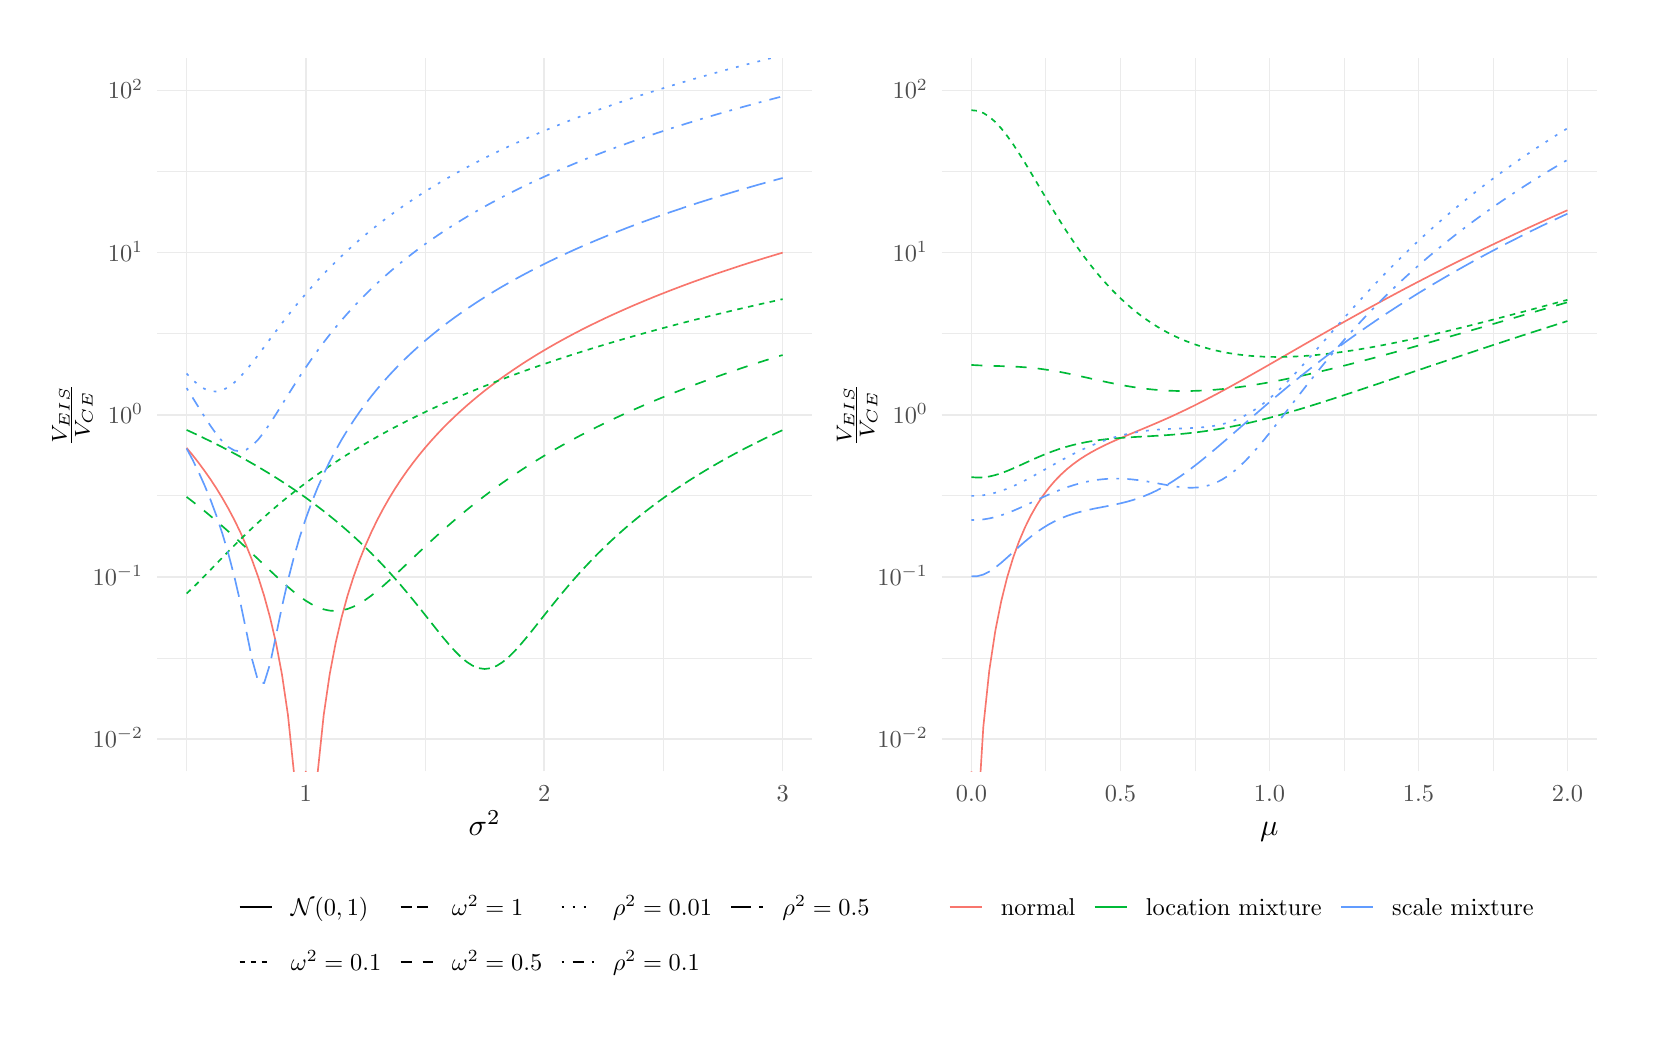
\begin{tikzpicture}[x=1pt,y=1pt]
\definecolor{fillColor}{RGB}{255,255,255}
\path[use as bounding box,fill=fillColor,fill opacity=0.00] (0,0) rectangle (578.16,361.35);
\begin{scope}
\path[clip] ( 46.66, 92.59) rectangle (283.58,350.35);
\definecolor{drawColor}{gray}{0.92}

\path[draw=drawColor,line width= 0.3pt,line join=round] ( 46.66,133.60) --
	(283.58,133.60);

\path[draw=drawColor,line width= 0.3pt,line join=round] ( 46.66,192.18) --
	(283.58,192.18);

\path[draw=drawColor,line width= 0.3pt,line join=round] ( 46.66,250.76) --
	(283.58,250.76);

\path[draw=drawColor,line width= 0.3pt,line join=round] ( 46.66,309.34) --
	(283.58,309.34);

\path[draw=drawColor,line width= 0.3pt,line join=round] ( 57.43, 92.59) --
	( 57.43,350.35);

\path[draw=drawColor,line width= 0.3pt,line join=round] (143.58, 92.59) --
	(143.58,350.35);

\path[draw=drawColor,line width= 0.3pt,line join=round] (229.74, 92.59) --
	(229.74,350.35);

\path[draw=drawColor,line width= 0.6pt,line join=round] ( 46.66,104.31) --
	(283.58,104.31);

\path[draw=drawColor,line width= 0.6pt,line join=round] ( 46.66,162.89) --
	(283.58,162.89);

\path[draw=drawColor,line width= 0.6pt,line join=round] ( 46.66,221.47) --
	(283.58,221.47);

\path[draw=drawColor,line width= 0.6pt,line join=round] ( 46.66,280.05) --
	(283.58,280.05);

\path[draw=drawColor,line width= 0.6pt,line join=round] ( 46.66,338.63) --
	(283.58,338.63);

\path[draw=drawColor,line width= 0.6pt,line join=round] (100.51, 92.59) --
	(100.51,350.35);

\path[draw=drawColor,line width= 0.6pt,line join=round] (186.66, 92.59) --
	(186.66,350.35);

\path[draw=drawColor,line width= 0.6pt,line join=round] (272.81, 92.59) --
	(272.81,350.35);
\definecolor{drawColor}{RGB}{248,118,109}

\path[draw=drawColor,line width= 0.6pt,line join=round] ( 57.43,209.51) --
	( 59.59,206.90) --
	( 61.74,204.15) --
	( 63.89,201.24) --
	( 66.05,198.16) --
	( 68.20,194.88) --
	( 70.35,191.37) --
	( 72.51,187.59) --
	( 74.66,183.52) --
	( 76.82,179.09) --
	( 78.97,174.25) --
	( 81.12,168.88) --
	( 83.28,162.89) --
	( 85.43,156.10) --
	( 87.58,148.25) --
	( 89.74,138.98) --
	( 91.89,127.62) --
	( 94.05,112.98) --
	( 96.20, 92.35) --
	( 98.35, 57.08) --
	(100.51, 92.59) --
	(102.66, 57.08) --
	(104.81, 92.35) --
	(106.97,112.98) --
	(109.12,127.62) --
	(111.28,138.98) --
	(113.43,148.25) --
	(115.58,156.10) --
	(117.74,162.89) --
	(119.89,168.88) --
	(122.05,174.25) --
	(124.20,179.09) --
	(126.35,183.52) --
	(128.51,187.59) --
	(130.66,191.37) --
	(132.81,194.88) --
	(134.97,198.16) --
	(137.12,201.24) --
	(139.28,204.15) --
	(141.43,206.90) --
	(143.58,209.51) --
	(145.74,212.00) --
	(147.89,214.36) --
	(150.04,216.63) --
	(152.20,218.79) --
	(154.35,220.87) --
	(156.51,222.86) --
	(158.66,224.78) --
	(160.81,226.63) --
	(162.97,228.42) --
	(165.12,230.15) --
	(167.27,231.81) --
	(169.43,233.43) --
	(171.58,235.00) --
	(173.74,236.51) --
	(175.89,237.99) --
	(178.04,239.42) --
	(180.20,240.82) --
	(182.35,242.17) --
	(184.51,243.50) --
	(186.66,244.78) --
	(188.81,246.04) --
	(190.97,247.27) --
	(193.12,248.46) --
	(195.27,249.63) --
	(197.43,250.78) --
	(199.58,251.90) --
	(201.74,252.99) --
	(203.89,254.06) --
	(206.04,255.11) --
	(208.20,256.14) --
	(210.35,257.15) --
	(212.50,258.13) --
	(214.66,259.10) --
	(216.81,260.05) --
	(218.97,260.99) --
	(221.12,261.90) --
	(223.27,262.80) --
	(225.43,263.69) --
	(227.58,264.56) --
	(229.74,265.41) --
	(231.89,266.26) --
	(234.04,267.08) --
	(236.20,267.90) --
	(238.35,268.70) --
	(240.50,269.49) --
	(242.66,270.26) --
	(244.81,271.03) --
	(246.97,271.78) --
	(249.12,272.53) --
	(251.27,273.26) --
	(253.43,273.98) --
	(255.58,274.69) --
	(257.73,275.39) --
	(259.89,276.09) --
	(262.04,276.77) --
	(264.20,277.44) --
	(266.35,278.11) --
	(268.50,278.76) --
	(270.66,279.41) --
	(272.81,280.05);
\definecolor{drawColor}{RGB}{0,186,56}

\path[draw=drawColor,line width= 0.6pt,dash pattern=on 2pt off 2pt ,line join=round] ( 57.43,156.87) --
	( 59.59,158.89) --
	( 61.74,161.01) --
	( 63.89,163.20) --
	( 66.05,165.41) --
	( 68.20,167.64) --
	( 70.35,169.87) --
	( 72.51,172.07) --
	( 74.66,174.24) --
	( 76.82,176.38) --
	( 78.97,178.48) --
	( 81.12,180.53) --
	( 83.28,182.53) --
	( 85.43,184.48) --
	( 87.58,186.39) --
	( 89.74,188.25) --
	( 91.89,190.06) --
	( 94.05,191.82) --
	( 96.20,193.53) --
	( 98.35,195.21) --
	(100.51,196.83) --
	(102.66,198.42) --
	(104.81,199.97) --
	(106.97,201.48) --
	(109.12,202.95) --
	(111.28,204.38) --
	(113.43,205.78) --
	(115.58,207.15) --
	(117.74,208.49) --
	(119.89,209.79) --
	(122.05,211.07) --
	(124.20,212.32) --
	(126.35,213.54) --
	(128.51,214.73) --
	(130.66,215.90) --
	(132.81,217.05) --
	(134.97,218.17) --
	(137.12,219.27) --
	(139.28,220.34) --
	(141.43,221.40) --
	(143.58,222.44) --
	(145.74,223.45) --
	(147.89,224.45) --
	(150.04,225.43) --
	(152.20,226.39) --
	(154.35,227.34) --
	(156.51,228.27) --
	(158.66,229.18) --
	(160.81,230.08) --
	(162.97,230.96) --
	(165.12,231.83) --
	(167.27,232.68) --
	(169.43,233.53) --
	(171.58,234.35) --
	(173.74,235.17) --
	(175.89,235.97) --
	(178.04,236.76) --
	(180.20,237.54) --
	(182.35,238.31) --
	(184.51,239.06) --
	(186.66,239.81) --
	(188.81,240.54) --
	(190.97,241.27) --
	(193.12,241.98) --
	(195.27,242.69) --
	(197.43,243.38) --
	(199.58,244.07) --
	(201.74,244.75) --
	(203.89,245.42) --
	(206.04,246.08) --
	(208.20,246.73) --
	(210.35,247.38) --
	(212.50,248.01) --
	(214.66,248.64) --
	(216.81,249.26) --
	(218.97,249.88) --
	(221.12,250.48) --
	(223.27,251.08) --
	(225.43,251.67) --
	(227.58,252.26) --
	(229.74,252.84) --
	(231.89,253.41) --
	(234.04,253.98) --
	(236.20,254.54) --
	(238.35,255.10) --
	(240.50,255.64) --
	(242.66,256.19) --
	(244.81,256.73) --
	(246.97,257.26) --
	(249.12,257.78) --
	(251.27,258.30) --
	(253.43,258.82) --
	(255.58,259.33) --
	(257.73,259.84) --
	(259.89,260.34) --
	(262.04,260.83) --
	(264.20,261.33) --
	(266.35,261.81) --
	(268.50,262.29) --
	(270.66,262.77) --
	(272.81,263.25);

\path[draw=drawColor,line width= 0.6pt,dash pattern=on 4pt off 2pt ,line join=round] ( 57.43,215.99) --
	( 59.59,215.00) --
	( 61.74,213.99) --
	( 63.89,212.95) --
	( 66.05,211.90) --
	( 68.20,210.83) --
	( 70.35,209.74) --
	( 72.51,208.62) --
	( 74.66,207.48) --
	( 76.82,206.31) --
	( 78.97,205.12) --
	( 81.12,203.90) --
	( 83.28,202.65) --
	( 85.43,201.37) --
	( 87.58,200.07) --
	( 89.74,198.73) --
	( 91.89,197.35) --
	( 94.05,195.94) --
	( 96.20,194.50) --
	( 98.35,193.01) --
	(100.51,191.49) --
	(102.66,189.92) --
	(104.81,188.31) --
	(106.97,186.65) --
	(109.12,184.94) --
	(111.28,183.19) --
	(113.43,181.37) --
	(115.58,179.50) --
	(117.74,177.57) --
	(119.89,175.58) --
	(122.05,173.53) --
	(124.20,171.41) --
	(126.35,169.22) --
	(128.51,166.95) --
	(130.66,164.62) --
	(132.81,162.21) --
	(134.97,159.73) --
	(137.12,157.18) --
	(139.28,154.56) --
	(141.43,151.89) --
	(143.58,149.18) --
	(145.74,146.46) --
	(147.89,143.74) --
	(150.04,141.07) --
	(152.20,138.51) --
	(154.35,136.12) --
	(156.51,133.97) --
	(158.66,132.17) --
	(160.81,130.79) --
	(162.97,129.92) --
	(165.12,129.61) --
	(167.27,129.88) --
	(169.43,130.72) --
	(171.58,132.07) --
	(173.74,133.85) --
	(175.89,135.98) --
	(178.04,138.36) --
	(180.20,140.91) --
	(182.35,143.57) --
	(184.51,146.29) --
	(186.66,149.02) --
	(188.81,151.73) --
	(190.97,154.40) --
	(193.12,157.02) --
	(195.27,159.57) --
	(197.43,162.06) --
	(199.58,164.47) --
	(201.74,166.81) --
	(203.89,169.08) --
	(206.04,171.28) --
	(208.20,173.40) --
	(210.35,175.46) --
	(212.50,177.45) --
	(214.66,179.39) --
	(216.81,181.26) --
	(218.97,183.08) --
	(221.12,184.84) --
	(223.27,186.55) --
	(225.43,188.21) --
	(227.58,189.82) --
	(229.74,191.39) --
	(231.89,192.92) --
	(234.04,194.41) --
	(236.20,195.86) --
	(238.35,197.27) --
	(240.50,198.64) --
	(242.66,199.98) --
	(244.81,201.29) --
	(246.97,202.57) --
	(249.12,203.82) --
	(251.27,205.04) --
	(253.43,206.24) --
	(255.58,207.41) --
	(257.73,208.55) --
	(259.89,209.67) --
	(262.04,210.76) --
	(264.20,211.84) --
	(266.35,212.89) --
	(268.50,213.92) --
	(270.66,214.94) --
	(272.81,215.93);

\path[draw=drawColor,line width= 0.6pt,dash pattern=on 4pt off 4pt ,line join=round] ( 57.43,191.79) --
	( 59.59,190.13) --
	( 61.74,188.43) --
	( 63.89,186.69) --
	( 66.05,184.90) --
	( 68.20,183.08) --
	( 70.35,181.21) --
	( 72.51,179.31) --
	( 74.66,177.36) --
	( 76.82,175.38) --
	( 78.97,173.37) --
	( 81.12,171.34) --
	( 83.28,169.29) --
	( 85.43,167.23) --
	( 87.58,165.18) --
	( 89.74,163.15) --
	( 91.89,161.17) --
	( 94.05,159.26) --
	( 96.20,157.45) --
	( 98.35,155.77) --
	(100.51,154.27) --
	(102.66,152.97) --
	(104.81,151.92) --
	(106.97,151.16) --
	(109.12,150.70) --
	(111.28,150.57) --
	(113.43,150.78) --
	(115.58,151.30) --
	(117.74,152.13) --
	(119.89,153.24) --
	(122.05,154.59) --
	(124.20,156.14) --
	(126.35,157.85) --
	(128.51,159.68) --
	(130.66,161.61) --
	(132.81,163.61) --
	(134.97,165.64) --
	(137.12,167.69) --
	(139.28,169.75) --
	(141.43,171.80) --
	(143.58,173.83) --
	(145.74,175.83) --
	(147.89,177.80) --
	(150.04,179.74) --
	(152.20,181.63) --
	(154.35,183.49) --
	(156.51,185.31) --
	(158.66,187.08) --
	(160.81,188.81) --
	(162.97,190.50) --
	(165.12,192.16) --
	(167.27,193.77) --
	(169.43,195.34) --
	(171.58,196.88) --
	(173.74,198.37) --
	(175.89,199.84) --
	(178.04,201.27) --
	(180.20,202.66) --
	(182.35,204.03) --
	(184.51,205.36) --
	(186.66,206.66) --
	(188.81,207.94) --
	(190.97,209.19) --
	(193.12,210.41) --
	(195.27,211.60) --
	(197.43,212.77) --
	(199.58,213.92) --
	(201.74,215.04) --
	(203.89,216.15) --
	(206.04,217.23) --
	(208.20,218.29) --
	(210.35,219.32) --
	(212.50,220.34) --
	(214.66,221.35) --
	(216.81,222.33) --
	(218.97,223.29) --
	(221.12,224.24) --
	(223.27,225.18) --
	(225.43,226.09) --
	(227.58,226.99) --
	(229.74,227.88) --
	(231.89,228.75) --
	(234.04,229.61) --
	(236.20,230.45) --
	(238.35,231.29) --
	(240.50,232.10) --
	(242.66,232.91) --
	(244.81,233.70) --
	(246.97,234.49) --
	(249.12,235.26) --
	(251.27,236.02) --
	(253.43,236.76) --
	(255.58,237.50) --
	(257.73,238.23) --
	(259.89,238.95) --
	(262.04,239.66) --
	(264.20,240.36) --
	(266.35,241.05) --
	(268.50,241.73) --
	(270.66,242.40) --
	(272.81,243.06);
\definecolor{drawColor}{RGB}{97,156,255}

\path[draw=drawColor,line width= 0.6pt,dash pattern=on 1pt off 3pt ,line join=round] ( 57.43,236.38) --
	( 59.59,234.11) --
	( 61.74,232.23) --
	( 63.89,230.84) --
	( 66.05,230.03) --
	( 68.20,229.86) --
	( 70.35,230.35) --
	( 72.51,231.46) --
	( 74.66,233.10) --
	( 76.82,235.19) --
	( 78.97,237.61) --
	( 81.12,240.26) --
	( 83.28,243.06) --
	( 85.43,245.93) --
	( 87.58,248.83) --
	( 89.74,251.71) --
	( 91.89,254.55) --
	( 94.05,257.33) --
	( 96.20,260.04) --
	( 98.35,262.67) --
	(100.51,265.21) --
	(102.66,267.68) --
	(104.81,270.06) --
	(106.97,272.37) --
	(109.12,274.59) --
	(111.28,276.74) --
	(113.43,278.82) --
	(115.58,280.84) --
	(117.74,282.78) --
	(119.89,284.67) --
	(122.05,286.50) --
	(124.20,288.27) --
	(126.35,289.98) --
	(128.51,291.65) --
	(130.66,293.27) --
	(132.81,294.84) --
	(134.97,296.37) --
	(137.12,297.86) --
	(139.28,299.31) --
	(141.43,300.72) --
	(143.58,302.10) --
	(145.74,303.44) --
	(147.89,304.75) --
	(150.04,306.03) --
	(152.20,307.28) --
	(154.35,308.50) --
	(156.51,309.70) --
	(158.66,310.86) --
	(160.81,312.01) --
	(162.97,313.12) --
	(165.12,314.22) --
	(167.27,315.29) --
	(169.43,316.34) --
	(171.58,317.37) --
	(173.74,318.39) --
	(175.89,319.38) --
	(178.04,320.35) --
	(180.20,321.31) --
	(182.35,322.25) --
	(184.51,323.17) --
	(186.66,324.07) --
	(188.81,324.96) --
	(190.97,325.84) --
	(193.12,326.70) --
	(195.27,327.55) --
	(197.43,328.38) --
	(199.58,329.20) --
	(201.74,330.01) --
	(203.89,330.81) --
	(206.04,331.59) --
	(208.20,332.36) --
	(210.35,333.12) --
	(212.50,333.87) --
	(214.66,334.61) --
	(216.81,335.34) --
	(218.97,336.06) --
	(221.12,336.76) --
	(223.27,337.46) --
	(225.43,338.15) --
	(227.58,338.83) --
	(229.74,339.50) --
	(231.89,340.17) --
	(234.04,340.82) --
	(236.20,341.47) --
	(238.35,342.11) --
	(240.50,342.74) --
	(242.66,343.36) --
	(244.81,343.97) --
	(246.97,344.58) --
	(249.12,345.18) --
	(251.27,345.78) --
	(253.43,346.37) --
	(255.58,346.95) --
	(257.73,347.52) --
	(259.89,348.09) --
	(262.04,348.65) --
	(264.20,349.20) --
	(266.35,349.75) --
	(268.50,350.30) --
	(270.66,350.84) --
	(272.81,351.37);

\path[draw=drawColor,line width= 0.6pt,dash pattern=on 1pt off 3pt on 4pt off 3pt ,line join=round] ( 57.43,231.11) --
	( 59.59,227.68) --
	( 61.74,224.21) --
	( 63.89,220.79) --
	( 66.05,217.49) --
	( 68.20,214.46) --
	( 70.35,211.84) --
	( 72.51,209.82) --
	( 74.66,208.58) --
	( 76.82,208.24) --
	( 78.97,208.83) --
	( 81.12,210.29) --
	( 83.28,212.49) --
	( 85.43,215.23) --
	( 87.58,218.35) --
	( 89.74,221.70) --
	( 91.89,225.14) --
	( 94.05,228.60) --
	( 96.20,232.02) --
	( 98.35,235.36) --
	(100.51,238.60) --
	(102.66,241.72) --
	(104.81,244.73) --
	(106.97,247.63) --
	(109.12,250.40) --
	(111.28,253.07) --
	(113.43,255.63) --
	(115.58,258.09) --
	(117.74,260.45) --
	(119.89,262.73) --
	(122.05,264.92) --
	(124.20,267.03) --
	(126.35,269.06) --
	(128.51,271.02) --
	(130.66,272.92) --
	(132.81,274.76) --
	(134.97,276.53) --
	(137.12,278.25) --
	(139.28,279.92) --
	(141.43,281.54) --
	(143.58,283.11) --
	(145.74,284.63) --
	(147.89,286.12) --
	(150.04,287.56) --
	(152.20,288.97) --
	(154.35,290.34) --
	(156.51,291.67) --
	(158.66,292.98) --
	(160.81,294.25) --
	(162.97,295.49) --
	(165.12,296.70) --
	(167.27,297.89) --
	(169.43,299.04) --
	(171.58,300.18) --
	(173.74,301.29) --
	(175.89,302.38) --
	(178.04,303.44) --
	(180.20,304.48) --
	(182.35,305.51) --
	(184.51,306.51) --
	(186.66,307.49) --
	(188.81,308.46) --
	(190.97,309.41) --
	(193.12,310.34) --
	(195.27,311.25) --
	(197.43,312.15) --
	(199.58,313.04) --
	(201.74,313.91) --
	(203.89,314.76) --
	(206.04,315.60) --
	(208.20,316.43) --
	(210.35,317.24) --
	(212.50,318.04) --
	(214.66,318.83) --
	(216.81,319.61) --
	(218.97,320.38) --
	(221.12,321.13) --
	(223.27,321.87) --
	(225.43,322.61) --
	(227.58,323.33) --
	(229.74,324.04) --
	(231.89,324.75) --
	(234.04,325.44) --
	(236.20,326.12) --
	(238.35,326.80) --
	(240.50,327.46) --
	(242.66,328.12) --
	(244.81,328.77) --
	(246.97,329.41) --
	(249.12,330.05) --
	(251.27,330.67) --
	(253.43,331.29) --
	(255.58,331.90) --
	(257.73,332.51) --
	(259.89,333.10) --
	(262.04,333.69) --
	(264.20,334.28) --
	(266.35,334.85) --
	(268.50,335.42) --
	(270.66,335.99) --
	(272.81,336.54);

\path[draw=drawColor,line width= 0.6pt,dash pattern=on 7pt off 3pt ,line join=round] ( 57.43,209.27) --
	( 59.59,205.22) --
	( 61.74,200.82) --
	( 63.89,196.04) --
	( 66.05,190.80) --
	( 68.20,185.00) --
	( 70.35,178.54) --
	( 72.51,171.28) --
	( 74.66,163.07) --
	( 76.82,153.77) --
	( 78.97,143.46) --
	( 81.12,132.99) --
	( 83.28,125.18) --
	( 85.43,124.48) --
	( 87.58,131.42) --
	( 89.74,141.72) --
	( 91.89,152.14) --
	( 94.05,161.62) --
	( 96.20,170.01) --
	( 98.35,177.41) --
	(100.51,183.99) --
	(102.66,189.89) --
	(104.81,195.22) --
	(106.97,200.07) --
	(109.12,204.52) --
	(111.28,208.63) --
	(113.43,212.44) --
	(115.58,215.99) --
	(117.74,219.32) --
	(119.89,222.45) --
	(122.05,225.40) --
	(124.20,228.19) --
	(126.35,230.84) --
	(128.51,233.36) --
	(130.66,235.76) --
	(132.81,238.05) --
	(134.97,240.25) --
	(137.12,242.36) --
	(139.28,244.38) --
	(141.43,246.33) --
	(143.58,248.20) --
	(145.74,250.01) --
	(147.89,251.76) --
	(150.04,253.45) --
	(152.20,255.09) --
	(154.35,256.67) --
	(156.51,258.21) --
	(158.66,259.70) --
	(160.81,261.15) --
	(162.97,262.56) --
	(165.12,263.94) --
	(167.27,265.27) --
	(169.43,266.58) --
	(171.58,267.85) --
	(173.74,269.08) --
	(175.89,270.29) --
	(178.04,271.48) --
	(180.20,272.63) --
	(182.35,273.76) --
	(184.51,274.87) --
	(186.66,275.95) --
	(188.81,277.01) --
	(190.97,278.05) --
	(193.12,279.06) --
	(195.27,280.06) --
	(197.43,281.04) --
	(199.58,282.00) --
	(201.74,282.94) --
	(203.89,283.86) --
	(206.04,284.77) --
	(208.20,285.66) --
	(210.35,286.54) --
	(212.50,287.40) --
	(214.66,288.25) --
	(216.81,289.09) --
	(218.97,289.91) --
	(221.12,290.71) --
	(223.27,291.51) --
	(225.43,292.29) --
	(227.58,293.06) --
	(229.74,293.82) --
	(231.89,294.57) --
	(234.04,295.31) --
	(236.20,296.03) --
	(238.35,296.75) --
	(240.50,297.46) --
	(242.66,298.16) --
	(244.81,298.84) --
	(246.97,299.52) --
	(249.12,300.19) --
	(251.27,300.85) --
	(253.43,301.50) --
	(255.58,302.15) --
	(257.73,302.78) --
	(259.89,303.41) --
	(262.04,304.03) --
	(264.20,304.65) --
	(266.35,305.25) --
	(268.50,305.85) --
	(270.66,306.44) --
	(272.81,307.03);
\end{scope}
\begin{scope}
\path[clip] (  0.00,  0.00) rectangle (578.16,361.35);
\definecolor{drawColor}{gray}{0.30}

\node[text=drawColor,anchor=base east,inner sep=0pt, outer sep=0pt, scale=  0.88] at ( 41.71,101.28) {$10^{-2}$};

\node[text=drawColor,anchor=base east,inner sep=0pt, outer sep=0pt, scale=  0.88] at ( 41.71,159.86) {$10^{-1}$};

\node[text=drawColor,anchor=base east,inner sep=0pt, outer sep=0pt, scale=  0.88] at ( 41.71,218.44) {$10^{0}$};

\node[text=drawColor,anchor=base east,inner sep=0pt, outer sep=0pt, scale=  0.88] at ( 41.71,277.02) {$10^{1}$};

\node[text=drawColor,anchor=base east,inner sep=0pt, outer sep=0pt, scale=  0.88] at ( 41.71,335.60) {$10^{2}$};
\end{scope}
\begin{scope}
\path[clip] (  0.00,  0.00) rectangle (578.16,361.35);
\definecolor{drawColor}{gray}{0.30}

\node[text=drawColor,anchor=base,inner sep=0pt, outer sep=0pt, scale=  0.88] at (100.51, 81.58) {1};

\node[text=drawColor,anchor=base,inner sep=0pt, outer sep=0pt, scale=  0.88] at (186.66, 81.58) {2};

\node[text=drawColor,anchor=base,inner sep=0pt, outer sep=0pt, scale=  0.88] at (272.81, 81.58) {3};
\end{scope}
\begin{scope}
\path[clip] (  0.00,  0.00) rectangle (578.16,361.35);
\definecolor{drawColor}{RGB}{0,0,0}

\node[text=drawColor,anchor=base,inner sep=0pt, outer sep=0pt, scale=  1.10] at (165.12, 69.55) {$\sigma^2$};
\end{scope}
\begin{scope}
\path[clip] (  0.00,  0.00) rectangle (578.16,361.35);
\definecolor{drawColor}{RGB}{0,0,0}

\node[text=drawColor,rotate= 90.00,anchor=base,inner sep=0pt, outer sep=0pt, scale=  1.10] at ( 18.58,221.47) {$\frac{V_{EIS}}{V_{CE}}$};
\end{scope}
\begin{scope}
\path[clip] (330.24, 92.59) rectangle (567.16,350.35);
\definecolor{drawColor}{gray}{0.92}

\path[draw=drawColor,line width= 0.3pt,line join=round] (330.24,133.60) --
	(567.16,133.60);

\path[draw=drawColor,line width= 0.3pt,line join=round] (330.24,192.18) --
	(567.16,192.18);

\path[draw=drawColor,line width= 0.3pt,line join=round] (330.24,250.76) --
	(567.16,250.76);

\path[draw=drawColor,line width= 0.3pt,line join=round] (330.24,309.34) --
	(567.16,309.34);

\path[draw=drawColor,line width= 0.3pt,line join=round] (367.93, 92.59) --
	(367.93,350.35);

\path[draw=drawColor,line width= 0.3pt,line join=round] (421.78, 92.59) --
	(421.78,350.35);

\path[draw=drawColor,line width= 0.3pt,line join=round] (475.62, 92.59) --
	(475.62,350.35);

\path[draw=drawColor,line width= 0.3pt,line join=round] (529.47, 92.59) --
	(529.47,350.35);

\path[draw=drawColor,line width= 0.6pt,line join=round] (330.24,104.31) --
	(567.16,104.31);

\path[draw=drawColor,line width= 0.6pt,line join=round] (330.24,162.89) --
	(567.16,162.89);

\path[draw=drawColor,line width= 0.6pt,line join=round] (330.24,221.47) --
	(567.16,221.47);

\path[draw=drawColor,line width= 0.6pt,line join=round] (330.24,280.05) --
	(567.16,280.05);

\path[draw=drawColor,line width= 0.6pt,line join=round] (330.24,338.63) --
	(567.16,338.63);

\path[draw=drawColor,line width= 0.6pt,line join=round] (341.01, 92.59) --
	(341.01,350.35);

\path[draw=drawColor,line width= 0.6pt,line join=round] (394.86, 92.59) --
	(394.86,350.35);

\path[draw=drawColor,line width= 0.6pt,line join=round] (448.70, 92.59) --
	(448.70,350.35);

\path[draw=drawColor,line width= 0.6pt,line join=round] (502.55, 92.59) --
	(502.55,350.35);

\path[draw=drawColor,line width= 0.6pt,line join=round] (556.39, 92.59) --
	(556.39,350.35);
\definecolor{drawColor}{RGB}{248,118,109}

\path[draw=drawColor,line width= 0.6pt,line join=round] (341.01, 92.59) --
	(343.17, 73.62) --
	(345.32,108.70) --
	(347.47,129.03) --
	(349.63,143.25) --
	(351.78,154.07) --
	(353.93,162.71) --
	(356.09,169.81) --
	(358.24,175.76) --
	(360.40,180.82) --
	(362.55,185.16) --
	(364.70,188.93) --
	(366.86,192.20) --
	(369.01,195.06) --
	(371.16,197.58) --
	(373.32,199.80) --
	(375.47,201.77) --
	(377.63,203.52) --
	(379.78,205.09) --
	(381.93,206.51) --
	(384.09,207.79) --
	(386.24,208.97) --
	(388.39,210.07) --
	(390.55,211.10) --
	(392.70,212.07) --
	(394.86,213.01) --
	(397.01,213.92) --
	(399.16,214.82) --
	(401.32,215.72) --
	(403.47,216.61) --
	(405.63,217.52) --
	(407.78,218.43) --
	(409.93,219.37) --
	(412.09,220.32) --
	(414.24,221.30) --
	(416.39,222.31) --
	(418.55,223.33) --
	(420.70,224.38) --
	(422.86,225.46) --
	(425.01,226.55) --
	(427.16,227.67) --
	(429.32,228.80) --
	(431.47,229.96) --
	(433.62,231.13) --
	(435.78,232.31) --
	(437.93,233.51) --
	(440.09,234.72) --
	(442.24,235.94) --
	(444.39,237.16) --
	(446.55,238.39) --
	(448.70,239.62) --
	(450.85,240.86) --
	(453.01,242.10) --
	(455.16,243.34) --
	(457.32,244.58) --
	(459.47,245.82) --
	(461.62,247.06) --
	(463.78,248.29) --
	(465.93,249.53) --
	(468.09,250.75) --
	(470.24,251.98) --
	(472.39,253.19) --
	(474.55,254.41) --
	(476.70,255.61) --
	(478.85,256.81) --
	(481.01,258.01) --
	(483.16,259.20) --
	(485.32,260.38) --
	(487.47,261.55) --
	(489.62,262.72) --
	(491.78,263.88) --
	(493.93,265.03) --
	(496.08,266.18) --
	(498.24,267.32) --
	(500.39,268.45) --
	(502.55,269.57) --
	(504.70,270.69) --
	(506.85,271.80) --
	(509.01,272.90) --
	(511.16,273.99) --
	(513.32,275.08) --
	(515.47,276.16) --
	(517.62,277.23) --
	(519.78,278.30) --
	(521.93,279.36) --
	(524.08,280.41) --
	(526.24,281.45) --
	(528.39,282.49) --
	(530.55,283.52) --
	(532.70,284.55) --
	(534.85,285.56) --
	(537.01,286.58) --
	(539.16,287.58) --
	(541.31,288.58) --
	(543.47,289.57) --
	(545.62,290.55) --
	(547.78,291.53) --
	(549.93,292.50) --
	(552.08,293.47) --
	(554.24,294.43) --
	(556.39,295.38);
\definecolor{drawColor}{RGB}{0,186,56}

\path[draw=drawColor,line width= 0.6pt,dash pattern=on 2pt off 2pt ,line join=round] (341.01,331.52) --
	(343.17,331.31) --
	(345.32,330.52) --
	(347.47,329.16) --
	(349.63,327.29) --
	(351.78,324.96) --
	(353.93,322.24) --
	(356.09,319.21) --
	(358.24,315.92) --
	(360.40,312.46) --
	(362.55,308.89) --
	(364.70,305.26) --
	(366.86,301.63) --
	(369.01,298.02) --
	(371.16,294.47) --
	(373.32,291.01) --
	(375.47,287.65) --
	(377.63,284.42) --
	(379.78,281.32) --
	(381.93,278.36) --
	(384.09,275.54) --
	(386.24,272.87) --
	(388.39,270.34) --
	(390.55,267.95) --
	(392.70,265.70) --
	(394.86,263.59) --
	(397.01,261.61) --
	(399.16,259.76) --
	(401.32,258.03) --
	(403.47,256.42) --
	(405.63,254.93) --
	(407.78,253.54) --
	(409.93,252.26) --
	(412.09,251.08) --
	(414.24,250.00) --
	(416.39,249.01) --
	(418.55,248.10) --
	(420.70,247.27) --
	(422.86,246.53) --
	(425.01,245.85) --
	(427.16,245.25) --
	(429.32,244.71) --
	(431.47,244.24) --
	(433.62,243.83) --
	(435.78,243.48) --
	(437.93,243.18) --
	(440.09,242.93) --
	(442.24,242.73) --
	(444.39,242.57) --
	(446.55,242.46) --
	(448.70,242.39) --
	(450.85,242.37) --
	(453.01,242.37) --
	(455.16,242.42) --
	(457.32,242.49) --
	(459.47,242.60) --
	(461.62,242.74) --
	(463.78,242.91) --
	(465.93,243.10) --
	(468.09,243.32) --
	(470.24,243.56) --
	(472.39,243.83) --
	(474.55,244.11) --
	(476.70,244.42) --
	(478.85,244.74) --
	(481.01,245.08) --
	(483.16,245.44) --
	(485.32,245.82) --
	(487.47,246.21) --
	(489.62,246.62) --
	(491.78,247.03) --
	(493.93,247.47) --
	(496.08,247.91) --
	(498.24,248.36) --
	(500.39,248.83) --
	(502.55,249.30) --
	(504.70,249.78) --
	(506.85,250.28) --
	(509.01,250.77) --
	(511.16,251.28) --
	(513.32,251.80) --
	(515.47,252.32) --
	(517.62,252.85) --
	(519.78,253.38) --
	(521.93,253.92) --
	(524.08,254.46) --
	(526.24,255.01) --
	(528.39,255.56) --
	(530.55,256.12) --
	(532.70,256.68) --
	(534.85,257.24) --
	(537.01,257.81) --
	(539.16,258.38) --
	(541.31,258.95) --
	(543.47,259.52) --
	(545.62,260.10) --
	(547.78,260.68) --
	(549.93,261.26) --
	(552.08,261.84) --
	(554.24,262.42) --
	(556.39,263.00);

\path[draw=drawColor,line width= 0.6pt,dash pattern=on 4pt off 2pt ,line join=round] (341.01,198.93) --
	(343.17,198.77) --
	(345.32,198.85) --
	(347.47,199.16) --
	(349.63,199.68) --
	(351.78,200.35) --
	(353.93,201.17) --
	(356.09,202.08) --
	(358.24,203.04) --
	(360.40,204.03) --
	(362.55,205.01) --
	(364.70,205.97) --
	(366.86,206.89) --
	(369.01,207.75) --
	(371.16,208.55) --
	(373.32,209.28) --
	(375.47,209.93) --
	(377.63,210.52) --
	(379.78,211.03) --
	(381.93,211.48) --
	(384.09,211.87) --
	(386.24,212.20) --
	(388.39,212.48) --
	(390.55,212.73) --
	(392.70,212.93) --
	(394.86,213.10) --
	(397.01,213.25) --
	(399.16,213.38) --
	(401.32,213.51) --
	(403.47,213.62) --
	(405.63,213.74) --
	(407.78,213.87) --
	(409.93,214.00) --
	(412.09,214.15) --
	(414.24,214.31) --
	(416.39,214.50) --
	(418.55,214.71) --
	(420.70,214.94) --
	(422.86,215.20) --
	(425.01,215.48) --
	(427.16,215.80) --
	(429.32,216.14) --
	(431.47,216.51) --
	(433.62,216.91) --
	(435.78,217.33) --
	(437.93,217.78) --
	(440.09,218.25) --
	(442.24,218.75) --
	(444.39,219.27) --
	(446.55,219.81) --
	(448.70,220.37) --
	(450.85,220.95) --
	(453.01,221.55) --
	(455.16,222.16) --
	(457.32,222.79) --
	(459.47,223.43) --
	(461.62,224.08) --
	(463.78,224.75) --
	(465.93,225.42) --
	(468.09,226.11) --
	(470.24,226.80) --
	(472.39,227.49) --
	(474.55,228.19) --
	(476.70,228.90) --
	(478.85,229.62) --
	(481.01,230.33) --
	(483.16,231.06) --
	(485.32,231.78) --
	(487.47,232.50) --
	(489.62,233.23) --
	(491.78,233.96) --
	(493.93,234.69) --
	(496.08,235.42) --
	(498.24,236.15) --
	(500.39,236.88) --
	(502.55,237.61) --
	(504.70,238.34) --
	(506.85,239.07) --
	(509.01,239.80) --
	(511.16,240.52) --
	(513.32,241.25) --
	(515.47,241.98) --
	(517.62,242.70) --
	(519.78,243.42) --
	(521.93,244.14) --
	(524.08,244.86) --
	(526.24,245.57) --
	(528.39,246.28) --
	(530.55,246.99) --
	(532.70,247.70) --
	(534.85,248.41) --
	(537.01,249.11) --
	(539.16,249.81) --
	(541.31,250.51) --
	(543.47,251.21) --
	(545.62,251.90) --
	(547.78,252.59) --
	(549.93,253.28) --
	(552.08,253.96) --
	(554.24,254.65) --
	(556.39,255.33);

\path[draw=drawColor,line width= 0.6pt,dash pattern=on 4pt off 4pt ,line join=round] (341.01,239.47) --
	(343.17,239.35) --
	(345.32,239.26) --
	(347.47,239.18) --
	(349.63,239.11) --
	(351.78,239.05) --
	(353.93,238.98) --
	(356.09,238.89) --
	(358.24,238.78) --
	(360.40,238.63) --
	(362.55,238.45) --
	(364.70,238.22) --
	(366.86,237.94) --
	(369.01,237.63) --
	(371.16,237.28) --
	(373.32,236.89) --
	(375.47,236.46) --
	(377.63,236.01) --
	(379.78,235.54) --
	(381.93,235.06) --
	(384.09,234.57) --
	(386.24,234.08) --
	(388.39,233.61) --
	(390.55,233.14) --
	(392.70,232.70) --
	(394.86,232.28) --
	(397.01,231.89) --
	(399.16,231.53) --
	(401.32,231.22) --
	(403.47,230.93) --
	(405.63,230.68) --
	(407.78,230.48) --
	(409.93,230.31) --
	(412.09,230.19) --
	(414.24,230.10) --
	(416.39,230.06) --
	(418.55,230.05) --
	(420.70,230.08) --
	(422.86,230.15) --
	(425.01,230.25) --
	(427.16,230.38) --
	(429.32,230.54) --
	(431.47,230.74) --
	(433.62,230.96) --
	(435.78,231.21) --
	(437.93,231.49) --
	(440.09,231.79) --
	(442.24,232.11) --
	(444.39,232.46) --
	(446.55,232.82) --
	(448.70,233.20) --
	(450.85,233.60) --
	(453.01,234.02) --
	(455.16,234.46) --
	(457.32,234.90) --
	(459.47,235.37) --
	(461.62,235.84) --
	(463.78,236.33) --
	(465.93,236.83) --
	(468.09,237.34) --
	(470.24,237.86) --
	(472.39,238.39) --
	(474.55,238.92) --
	(476.70,239.47) --
	(478.85,240.02) --
	(481.01,240.58) --
	(483.16,241.15) --
	(485.32,241.72) --
	(487.47,242.30) --
	(489.62,242.88) --
	(491.78,243.47) --
	(493.93,244.06) --
	(496.08,244.66) --
	(498.24,245.26) --
	(500.39,245.87) --
	(502.55,246.48) --
	(504.70,247.09) --
	(506.85,247.70) --
	(509.01,248.32) --
	(511.16,248.94) --
	(513.32,249.56) --
	(515.47,250.18) --
	(517.62,250.80) --
	(519.78,251.43) --
	(521.93,252.05) --
	(524.08,252.68) --
	(526.24,253.31) --
	(528.39,253.94) --
	(530.55,254.57) --
	(532.70,255.20) --
	(534.85,255.83) --
	(537.01,256.45) --
	(539.16,257.09) --
	(541.31,257.72) --
	(543.47,258.35) --
	(545.62,258.98) --
	(547.78,259.61) --
	(549.93,260.23) --
	(552.08,260.86) --
	(554.24,261.49) --
	(556.39,262.11);
\definecolor{drawColor}{RGB}{97,156,255}

\path[draw=drawColor,line width= 0.6pt,dash pattern=on 1pt off 3pt ,line join=round] (341.01,192.15) --
	(343.17,192.20) --
	(345.32,192.40) --
	(347.47,192.77) --
	(349.63,193.29) --
	(351.78,193.95) --
	(353.93,194.75) --
	(356.09,195.66) --
	(358.24,196.67) --
	(360.40,197.75) --
	(362.55,198.90) --
	(364.70,200.08) --
	(366.86,201.29) --
	(369.01,202.51) --
	(371.16,203.72) --
	(373.32,204.91) --
	(375.47,206.07) --
	(377.63,207.19) --
	(379.78,208.26) --
	(381.93,209.27) --
	(384.09,210.22) --
	(386.24,211.10) --
	(388.39,211.92) --
	(390.55,212.66) --
	(392.70,213.33) --
	(394.86,213.92) --
	(397.01,214.45) --
	(399.16,214.90) --
	(401.32,215.28) --
	(403.47,215.60) --
	(405.63,215.86) --
	(407.78,216.07) --
	(409.93,216.22) --
	(412.09,216.34) --
	(414.24,216.43) --
	(416.39,216.51) --
	(418.55,216.59) --
	(420.70,216.68) --
	(422.86,216.81) --
	(425.01,216.98) --
	(427.16,217.23) --
	(429.32,217.56) --
	(431.47,218.01) --
	(433.62,218.60) --
	(435.78,219.33) --
	(437.93,220.23) --
	(440.09,221.30) --
	(442.24,222.54) --
	(444.39,223.97) --
	(446.55,225.56) --
	(448.70,227.32) --
	(450.85,229.22) --
	(453.01,231.26) --
	(455.16,233.41) --
	(457.32,235.66) --
	(459.47,237.98) --
	(461.62,240.36) --
	(463.78,242.79) --
	(465.93,245.24) --
	(468.09,247.72) --
	(470.24,250.19) --
	(472.39,252.67) --
	(474.55,255.13) --
	(476.70,257.57) --
	(478.85,259.99) --
	(481.01,262.38) --
	(483.16,264.74) --
	(485.32,267.06) --
	(487.47,269.35) --
	(489.62,271.60) --
	(491.78,273.82) --
	(493.93,276.00) --
	(496.08,278.14) --
	(498.24,280.24) --
	(500.39,282.30) --
	(502.55,284.33) --
	(504.70,286.32) --
	(506.85,288.27) --
	(509.01,290.19) --
	(511.16,292.07) --
	(513.32,293.92) --
	(515.47,295.74) --
	(517.62,297.52) --
	(519.78,299.27) --
	(521.93,300.99) --
	(524.08,302.68) --
	(526.24,304.34) --
	(528.39,305.97) --
	(530.55,307.58) --
	(532.70,309.16) --
	(534.85,310.71) --
	(537.01,312.24) --
	(539.16,313.75) --
	(541.31,315.23) --
	(543.47,316.68) --
	(545.62,318.12) --
	(547.78,319.53) --
	(549.93,320.92) --
	(552.08,322.30) --
	(554.24,323.65) --
	(556.39,324.98);

\path[draw=drawColor,line width= 0.6pt,dash pattern=on 1pt off 3pt on 4pt off 3pt ,line join=round] (341.01,183.46) --
	(343.17,183.48) --
	(345.32,183.66) --
	(347.47,184.01) --
	(349.63,184.51) --
	(351.78,185.14) --
	(353.93,185.90) --
	(356.09,186.76) --
	(358.24,187.69) --
	(360.40,188.68) --
	(362.55,189.68) --
	(364.70,190.70) --
	(366.86,191.70) --
	(369.01,192.66) --
	(371.16,193.59) --
	(373.32,194.45) --
	(375.47,195.24) --
	(377.63,195.95) --
	(379.78,196.58) --
	(381.93,197.12) --
	(384.09,197.56) --
	(386.24,197.92) --
	(388.39,198.17) --
	(390.55,198.34) --
	(392.70,198.41) --
	(394.86,198.39) --
	(397.01,198.28) --
	(399.16,198.10) --
	(401.32,197.85) --
	(403.47,197.53) --
	(405.63,197.18) --
	(407.78,196.78) --
	(409.93,196.38) --
	(412.09,195.99) --
	(414.24,195.63) --
	(416.39,195.34) --
	(418.55,195.15) --
	(420.70,195.10) --
	(422.86,195.21) --
	(425.01,195.53) --
	(427.16,196.08) --
	(429.32,196.89) --
	(431.47,197.97) --
	(433.62,199.33) --
	(435.78,200.94) --
	(437.93,202.80) --
	(440.09,204.89) --
	(442.24,207.17) --
	(444.39,209.60) --
	(446.55,212.17) --
	(448.70,214.83) --
	(450.85,217.55) --
	(453.01,220.32) --
	(455.16,223.11) --
	(457.32,225.90) --
	(459.47,228.68) --
	(461.62,231.44) --
	(463.78,234.17) --
	(465.93,236.87) --
	(468.09,239.52) --
	(470.24,242.12) --
	(472.39,244.68) --
	(474.55,247.18) --
	(476.70,249.64) --
	(478.85,252.04) --
	(481.01,254.40) --
	(483.16,256.71) --
	(485.32,258.96) --
	(487.47,261.17) --
	(489.62,263.34) --
	(491.78,265.45) --
	(493.93,267.53) --
	(496.08,269.56) --
	(498.24,271.55) --
	(500.39,273.50) --
	(502.55,275.40) --
	(504.70,277.28) --
	(506.85,279.11) --
	(509.01,280.91) --
	(511.16,282.68) --
	(513.32,284.41) --
	(515.47,286.11) --
	(517.62,287.78) --
	(519.78,289.43) --
	(521.93,291.04) --
	(524.08,292.62) --
	(526.24,294.18) --
	(528.39,295.71) --
	(530.55,297.22) --
	(532.70,298.70) --
	(534.85,300.15) --
	(537.01,301.59) --
	(539.16,303.00) --
	(541.31,304.39) --
	(543.47,305.76) --
	(545.62,307.11) --
	(547.78,308.44) --
	(549.93,309.75) --
	(552.08,311.04) --
	(554.24,312.32) --
	(556.39,313.57);

\path[draw=drawColor,line width= 0.6pt,dash pattern=on 7pt off 3pt ,line join=round] (341.01,163.08) --
	(343.17,163.15) --
	(345.32,163.73) --
	(347.47,164.79) --
	(349.63,166.24) --
	(351.78,167.98) --
	(353.93,169.88) --
	(356.09,171.84) --
	(358.24,173.81) --
	(360.40,175.69) --
	(362.55,177.46) --
	(364.70,179.09) --
	(366.86,180.56) --
	(369.01,181.87) --
	(371.16,183.02) --
	(373.32,184.02) --
	(375.47,184.88) --
	(377.63,185.62) --
	(379.78,186.25) --
	(381.93,186.80) --
	(384.09,187.28) --
	(386.24,187.72) --
	(388.39,188.13) --
	(390.55,188.55) --
	(392.70,188.98) --
	(394.86,189.46) --
	(397.01,189.99) --
	(399.16,190.60) --
	(401.32,191.30) --
	(403.47,192.10) --
	(405.63,193.00) --
	(407.78,194.01) --
	(409.93,195.14) --
	(412.09,196.37) --
	(414.24,197.71) --
	(416.39,199.14) --
	(418.55,200.66) --
	(420.70,202.27) --
	(422.86,203.93) --
	(425.01,205.66) --
	(427.16,207.43) --
	(429.32,209.24) --
	(431.47,211.08) --
	(433.62,212.94) --
	(435.78,214.81) --
	(437.93,216.69) --
	(440.09,218.57) --
	(442.24,220.44) --
	(444.39,222.31) --
	(446.55,224.17) --
	(448.70,226.02) --
	(450.85,227.84) --
	(453.01,229.65) --
	(455.16,231.45) --
	(457.32,233.21) --
	(459.47,234.96) --
	(461.62,236.69) --
	(463.78,238.40) --
	(465.93,240.08) --
	(468.09,241.74) --
	(470.24,243.38) --
	(472.39,244.99) --
	(474.55,246.58) --
	(476.70,248.15) --
	(478.85,249.70) --
	(481.01,251.23) --
	(483.16,252.73) --
	(485.32,254.22) --
	(487.47,255.69) --
	(489.62,257.13) --
	(491.78,258.56) --
	(493.93,259.96) --
	(496.08,261.35) --
	(498.24,262.72) --
	(500.39,264.07) --
	(502.55,265.41) --
	(504.70,266.72) --
	(506.85,268.02) --
	(509.01,269.31) --
	(511.16,270.58) --
	(513.32,271.83) --
	(515.47,273.07) --
	(517.62,274.29) --
	(519.78,275.50) --
	(521.93,276.70) --
	(524.08,277.88) --
	(526.24,279.05) --
	(528.39,280.20) --
	(530.55,281.34) --
	(532.70,282.47) --
	(534.85,283.59) --
	(537.01,284.69) --
	(539.16,285.78) --
	(541.31,286.87) --
	(543.47,287.94) --
	(545.62,288.99) --
	(547.78,290.04) --
	(549.93,291.08) --
	(552.08,292.11) --
	(554.24,293.12) --
	(556.39,294.13);
\end{scope}
\begin{scope}
\path[clip] (  0.00,  0.00) rectangle (578.16,361.35);
\definecolor{drawColor}{gray}{0.30}

\node[text=drawColor,anchor=base east,inner sep=0pt, outer sep=0pt, scale=  0.88] at (325.29,101.28) {$10^{-2}$};

\node[text=drawColor,anchor=base east,inner sep=0pt, outer sep=0pt, scale=  0.88] at (325.29,159.86) {$10^{-1}$};

\node[text=drawColor,anchor=base east,inner sep=0pt, outer sep=0pt, scale=  0.88] at (325.29,218.44) {$10^{0}$};

\node[text=drawColor,anchor=base east,inner sep=0pt, outer sep=0pt, scale=  0.88] at (325.29,277.02) {$10^{1}$};

\node[text=drawColor,anchor=base east,inner sep=0pt, outer sep=0pt, scale=  0.88] at (325.29,335.60) {$10^{2}$};
\end{scope}
\begin{scope}
\path[clip] (  0.00,  0.00) rectangle (578.16,361.35);
\definecolor{drawColor}{gray}{0.30}

\node[text=drawColor,anchor=base,inner sep=0pt, outer sep=0pt, scale=  0.88] at (341.01, 81.58) {0.0};

\node[text=drawColor,anchor=base,inner sep=0pt, outer sep=0pt, scale=  0.88] at (394.86, 81.58) {0.5};

\node[text=drawColor,anchor=base,inner sep=0pt, outer sep=0pt, scale=  0.88] at (448.70, 81.58) {1.0};

\node[text=drawColor,anchor=base,inner sep=0pt, outer sep=0pt, scale=  0.88] at (502.55, 81.58) {1.5};

\node[text=drawColor,anchor=base,inner sep=0pt, outer sep=0pt, scale=  0.88] at (556.39, 81.58) {2.0};
\end{scope}
\begin{scope}
\path[clip] (  0.00,  0.00) rectangle (578.16,361.35);
\definecolor{drawColor}{RGB}{0,0,0}

\node[text=drawColor,anchor=base,inner sep=0pt, outer sep=0pt, scale=  1.10] at (448.70, 69.55) {$\mu$};
\end{scope}
\begin{scope}
\path[clip] (  0.00,  0.00) rectangle (578.16,361.35);
\definecolor{drawColor}{RGB}{0,0,0}

\node[text=drawColor,rotate= 90.00,anchor=base,inner sep=0pt, outer sep=0pt, scale=  1.10] at (302.16,221.47) {$\frac{V_{EIS}}{V_{CE}}$};
\end{scope}
\begin{scope}
\path[clip] (  0.00,  0.00) rectangle (578.16,361.35);
\definecolor{drawColor}{RGB}{0,0,0}

\path[draw=drawColor,line width= 0.6pt,line join=round] ( 76.56, 43.68) -- ( 88.13, 43.68);
\end{scope}
\begin{scope}
\path[clip] (  0.00,  0.00) rectangle (578.16,361.35);
\definecolor{drawColor}{RGB}{0,0,0}

\path[draw=drawColor,line width= 0.6pt,dash pattern=on 2pt off 2pt ,line join=round] ( 76.56, 23.73) -- ( 88.13, 23.73);
\end{scope}
\begin{scope}
\path[clip] (  0.00,  0.00) rectangle (578.16,361.35);
\definecolor{drawColor}{RGB}{0,0,0}

\path[draw=drawColor,line width= 0.6pt,dash pattern=on 4pt off 2pt ,line join=round] (134.74, 43.68) -- (146.30, 43.68);
\end{scope}
\begin{scope}
\path[clip] (  0.00,  0.00) rectangle (578.16,361.35);
\definecolor{drawColor}{RGB}{0,0,0}

\path[draw=drawColor,line width= 0.6pt,dash pattern=on 4pt off 4pt ,line join=round] (134.74, 23.73) -- (146.30, 23.73);
\end{scope}
\begin{scope}
\path[clip] (  0.00,  0.00) rectangle (578.16,361.35);
\definecolor{drawColor}{RGB}{0,0,0}

\path[draw=drawColor,line width= 0.6pt,dash pattern=on 1pt off 3pt ,line join=round] (192.91, 43.68) -- (204.47, 43.68);
\end{scope}
\begin{scope}
\path[clip] (  0.00,  0.00) rectangle (578.16,361.35);
\definecolor{drawColor}{RGB}{0,0,0}

\path[draw=drawColor,line width= 0.6pt,dash pattern=on 1pt off 3pt on 4pt off 3pt ,line join=round] (192.91, 23.73) -- (204.47, 23.73);
\end{scope}
\begin{scope}
\path[clip] (  0.00,  0.00) rectangle (578.16,361.35);
\definecolor{drawColor}{RGB}{0,0,0}

\path[draw=drawColor,line width= 0.6pt,dash pattern=on 7pt off 3pt ,line join=round] (254.24, 43.68) -- (265.80, 43.68);
\end{scope}
\begin{scope}
\path[clip] (  0.00,  0.00) rectangle (578.16,361.35);
\definecolor{drawColor}{RGB}{0,0,0}

\node[text=drawColor,anchor=base west,inner sep=0pt, outer sep=0pt, scale=  0.88] at ( 95.07, 40.65) {$\mathcal N (0, 1)$};
\end{scope}
\begin{scope}
\path[clip] (  0.00,  0.00) rectangle (578.16,361.35);
\definecolor{drawColor}{RGB}{0,0,0}

\node[text=drawColor,anchor=base west,inner sep=0pt, outer sep=0pt, scale=  0.88] at ( 95.07, 20.70) {$\omega^2 = 0.1$};
\end{scope}
\begin{scope}
\path[clip] (  0.00,  0.00) rectangle (578.16,361.35);
\definecolor{drawColor}{RGB}{0,0,0}

\node[text=drawColor,anchor=base west,inner sep=0pt, outer sep=0pt, scale=  0.88] at (153.24, 40.65) {$\omega^2 = 1$};
\end{scope}
\begin{scope}
\path[clip] (  0.00,  0.00) rectangle (578.16,361.35);
\definecolor{drawColor}{RGB}{0,0,0}

\node[text=drawColor,anchor=base west,inner sep=0pt, outer sep=0pt, scale=  0.88] at (153.24, 20.70) {$\omega^2= 0.5$};
\end{scope}
\begin{scope}
\path[clip] (  0.00,  0.00) rectangle (578.16,361.35);
\definecolor{drawColor}{RGB}{0,0,0}

\node[text=drawColor,anchor=base west,inner sep=0pt, outer sep=0pt, scale=  0.88] at (211.42, 40.65) {$\rho^2 = 0.01$};
\end{scope}
\begin{scope}
\path[clip] (  0.00,  0.00) rectangle (578.16,361.35);
\definecolor{drawColor}{RGB}{0,0,0}

\node[text=drawColor,anchor=base west,inner sep=0pt, outer sep=0pt, scale=  0.88] at (211.42, 20.70) {$\rho^2 = 0.1$};
\end{scope}
\begin{scope}
\path[clip] (  0.00,  0.00) rectangle (578.16,361.35);
\definecolor{drawColor}{RGB}{0,0,0}

\node[text=drawColor,anchor=base west,inner sep=0pt, outer sep=0pt, scale=  0.88] at (272.75, 40.65) {$\rho^2 = 0.5$};
\end{scope}
\begin{scope}
\path[clip] (  0.00,  0.00) rectangle (578.16,361.35);
\definecolor{drawColor}{RGB}{248,118,109}

\path[draw=drawColor,line width= 0.6pt,line join=round] (333.17, 43.68) -- (344.73, 43.68);
\end{scope}
\begin{scope}
\path[clip] (  0.00,  0.00) rectangle (578.16,361.35);
\definecolor{drawColor}{RGB}{0,186,56}

\path[draw=drawColor,line width= 0.6pt,line join=round] (385.53, 43.68) -- (397.09, 43.68);
\end{scope}
\begin{scope}
\path[clip] (  0.00,  0.00) rectangle (578.16,361.35);
\definecolor{drawColor}{RGB}{97,156,255}

\path[draw=drawColor,line width= 0.6pt,line join=round] (474.55, 43.68) -- (486.11, 43.68);
\end{scope}
\begin{scope}
\path[clip] (  0.00,  0.00) rectangle (578.16,361.35);
\definecolor{drawColor}{RGB}{0,0,0}

\node[text=drawColor,anchor=base west,inner sep=0pt, outer sep=0pt, scale=  0.88] at (351.68, 40.65) {normal};
\end{scope}
\begin{scope}
\path[clip] (  0.00,  0.00) rectangle (578.16,361.35);
\definecolor{drawColor}{RGB}{0,0,0}

\node[text=drawColor,anchor=base west,inner sep=0pt, outer sep=0pt, scale=  0.88] at (404.04, 40.65) {location mixture};
\end{scope}
\begin{scope}
\path[clip] (  0.00,  0.00) rectangle (578.16,361.35);
\definecolor{drawColor}{RGB}{0,0,0}

\node[text=drawColor,anchor=base west,inner sep=0pt, outer sep=0pt, scale=  0.88] at (493.06, 40.65) {scale mixture};
\end{scope}
\end{tikzpicture}
%
        }
        \caption{Asymptotic relative efficiency $\frac{V_{\eis}}{V_{\ce}}$ for the normal distribution from \Cref{ex:univ-gaussian-s2-fixed} (left hand side) and \Cref{ex:univ-gaussian-mu-fixed} (right hand side). Here $\P$ is either the standard normal distribution, a Gaussian location mixture, or a Gaussian scale mixture. $\G_{\psi}$ is the normal distribution $\mathcal N(\mu, \sigma^{2})$, where either $\sigma^{2}$ is fixed (left) and $\mu$ determined by the \gls{cem} / \gls{eis}, or the other way around (right). Notice the log scale of the $y$-axis. As $\mu$ or $\sigma^{2}$ get close to their true values, \gls{eis} outperforms the \gls{cem} in terms of asymptotic variance, see \Cref{prop:eis-finite-sample}. }
        \label{fig:are}
    \end{figure}

    
    \paragraph{Normal distribution}
    If $\P = \mathcal N(0, \tau^{2})$ is a normal distribution, this reduces to
    \begin{align*}
        V_{\eis} &= \frac{5}{2} \left( \frac{\tau^{2}}{\sigma^{2}} - 1 \right)^{2} \frac{\sigma^{2}}{\tau^{2}} = \frac{5}{2} \frac{\left( V_{\ce} - 1\right)^{2}}{V_{\ce}}
    \end{align*}
    and so for $\tau^{2} = \sigma^{2}$ we have $V_{\eis} = 0$, so $\hpeis$ might converge faster than the standard $\mathcal O( N^{-\frac{1}{2}})$ rate. Indeed, in this case $\hpeis = \peis$ a.s. for $N > 1$, see \Cref{prop:eis-finite-sample}.

    %For importance sampling to be consistent, it is necessary that $\sigma^{2} > \frac{\tau^{2}}{2}$. The left-hand side of \Cref{fig:are} displays the behavior of the relative efficiency
    %$$
    %\frac{V_{\eis}}{V_{\ce}} = \frac{5}{2} \frac{(V_{\ce} - 1)^{2}}{V_{\ce}^{2}} = \frac{5}{2} \left( 1 - \frac{2}{V_{\ce}} + \frac{1}{V_{\ce}^2} \right).
    %$$
    
    \paragraph{Gaussian location mixture}
    Consider now the case where $\P = \frac{1}{2} \mathcal N(-1, \omega^{2}) + \frac{1}{2}\mathcal N(1, \omega^{2})$ is a Gaussian location mixture. The second moment is $\tau^{2} = 1 + \omega^{2} = -\frac{1}{2\pce}$. Unfortunately, there is no closed-form expression for many of the terms required for the analysis of \gls{eis}. Instead, we resort to a simulation study to determine the asymptotic variances and relative efficiencies for three different values of $\omega^{2} \in \{0.1, 0.5, 1.0\}$. 
    
    To this end we draw $M = 400$ times from the distribution of $\hpce$ and $\hpeis$, where we use $N=1\,000$ samples from the tractable $\P$ as importance samples\footnote{Code for all simulation studies is available in the associated GitHub repository, see \Cref{cha:reproducibility_and_code}.}. We only iterate a single time for both procedures. From individual estimates, we estimate the asymptotic variances $V_{\ce}$ and $V_{\eis}$ by the respective empirical variances, and determine the relative efficiency of \gls{eis} over the \gls{cem} as $ \frac{\hat V_{\eis}}{\hat V_{\ce}}$. Again, we vary the fixed variance of the proposals, $\sigma^{2}$, from $\frac{1}{2}$ to $3$. 
    To quantify uncertainty in these asymptotic relative efficiencies, we perform the non-parametric bootstrap with $10\,000$ samples to estimate their standard errors $\widehat{\text{se}}_{b}$. $M=400$ has been chosen to ensure that the relative bootstrap standard error $ \frac{\widehat{\text{se}}_{b}}{\hat V_{\eis} / \hat V_{\ce}}$ is less than $10\%$ across all simulations. 
    
    \paragraph{Gaussian scale mixture}
    Finally we consider $\P = \frac{1}{2} \left(\mathcal N \left( 0, 1 \right) + \mathcal N (0, \varepsilon^{-2}) \right)$ for $\varepsilon^{2} \in \{2, 10, 100\}$, a scale mixture similar to the one seen in \Cref{ex:la_failure}. Contrary to that example, we choose $\varepsilon$ big, making the $\mathcal N(0,1)$ component the one with large variance, to make importance sampling with $\sigma^{2}$ in the range considered consistent. 
    Here $\tau^{2} = \frac{1}{2} + \frac{1}{2\varepsilon^{2}}$. 
    Again, we estimate the asymptotic $V_{\eis}$ in the same way as for the Gaussian location mixture, with $M=100$ estimates using $N=1000$ samples each and obtain a Monte-Carlo standard error for the asymptotic variances of $1.1 \times 10^{-3}$.
\end{example}
\vspace{16pt}
Note that for fixed $\sigma^{2}$ the asymptotic variance of the \acrshort{cem} $V_{\ce}$ is the same in all of the examples considered, as we sample directly from the tractable $\P$, so $V_{\ce}$ only depends on $\P$ through its second moment $\tau^{2}$. 
The asymptotic variance of \acrshort{eis} however depends on both $\tau^{2}$ and $\gamma$, which depends on higher order moments of $\P$.

From the left-hand side of \Cref{fig:are} we can observe that in the case of $\P = \mathcal N(0,1)$ \acrshort{eis} has smaller asymptotic variance compared to the \acrshort{cem}, as long as $\sigma^{2}$ is not heavily misspecified. Indeed, if $\sigma^{2} = 1$ is correctly specified, by \Cref{prop:eis-finite-sample}, \acrshort{eis} has asymptotic variance $0$ and converges already for a single sample. 

Consider now the case where $\P$ is a Gaussian location mixture. For $\omega^{2} = 1$, the location mixture is unimodal with variance $2$ and \aeis outperforms the \acem in terms of asymptotic variance in the range considered. For the smaller values of $\omega^{2}$ considered here, the location mixture is bimodal. Close to the true variance $1 + \omega^{2}$, \aeis still outperforms the \acem. 

For the Gaussian scale mixture, the case is less clear. Here the true variance is $\frac{1}{2} + \frac{1}{2 \varepsilon^{2}}$. The location of the minimal relative efficiency is still close to this true variance, however, as $\varepsilon^{2}$ grows, the \acem starts to dominate \aeis. Additionally, recall from \Cref{ex:la_failure} that for large $\varepsilon^{2}$ \aeis becomes inadmissible. 

\begin{example}[univariate Gaussian, $\mu$ fixed]
    \label{ex:univ-gaussian-mu-fixed}
    Consider the same setup as in \Cref{ex:univ-gaussian-s2-fixed}, i.e. $\P$ is symmetric around $0$ with second moment $\tau^{2}$, but let $\G_{\psi} = \mathcal N(\mu, -\frac{1}{2\psi})$ be the single parameter natural exponential family of Gaussians with fixed mean $\mu$ and variance $\sigma^{2} = -\frac{1}{2 \psi}$. 
    
    Then
    $$
    \log g_{\psi}(x) = \psi T(x) + \frac{1}{2}\log \left( - 2 \psi \right) - \frac{1}{2} \log 2\pi
    $$
    for $T(x) = (x - \mu)^{2}$. Thus $\P T = \tau^{2} + \mu^{2}$ and $\cov_{\P} T = \nu - \tau^{4} + 4\tau^{2}\mu^{2}$ where $\nu = \P \operatorname{id}^{4}$ and $\tau^{2} = \P \id^{2}$. 
    %\paragraph{\Acrlong{cem}}

    By matching moments, we obtain $\pce = -\frac{1}{2(\tau^{2} + \mu^{2})}$ and $I(\pce) = \frac{1}{2\psi^{2}_\ce} = 2(\tau^{2} + \mu^{2})^{2}$. In total 
    \begin{align}
        V_{\ce} &= \frac{1}{4 (\tau^{2} + \mu^{2})^{4}} \left( \nu - \tau^{4} + 4\tau^{2}\mu^{2} \right)
    \end{align}

    %\paragraph{\Acrlong{eis}}
    For \gls{eis},
    \begin{align*}
    \peis &= \left( \cov_{\P} T \right)^{-1} \cov_{\P} \left( T, \log p \right) \\
        &= \left( \nu - \tau^{4} + 4\tau^{2}\mu^{2} \right)^{-1} \underbrace{\int p(x)((x-\mu)^{2}-\tau^{2} - \mu^{2})(\log p(x) - \P\log p(x)) \d x}_{=\gamma}.
    \end{align*}
    
    As $B_{\eis} = \cov_{\P} T ^{-1} = \left( \nu - \tau^{4} + 4 \tau^{2}\mu^{2} \right)^{-1}$, we have
    \begin{align*}
        V_{\eis} = \left( \nu - \tau^{4} + 4 \tau^{2}\mu^{2}\right)^{-2} \P \left( (\id - \mu)^{4} \left( \log p - \peis (\id - \mu)^{2} - \P \log p + \psi (\tau^{2} + \mu^{2}) \right)^{2} \right),
    \end{align*}
    where the last term is equal to $M_{\eis}$. 

    We now perform the same analysis as in \Cref{ex:univ-gaussian-s2-fixed}, the resulting ratio of asymptotic variances is displayed in the right-hand side of \Cref{fig:are}. In general, the variances $\sigma^{2}_{\ce} = -\frac{1}{2\pce}$ and $\sigma^{2}_{\eis} = -\frac{1}{2\peis}$ are different, so the ratio is no longer an asymptotic relative efficiency. However, it is still relevant as a measure of the relative speed of stochastic convergence of both methods. Additionally, we display the resulting optimal variances in \Cref{fig:cem_eis_sigma2}.

    \paragraph{Normal distribution}
    For the normal distribution $\P = \mathcal N (0, \tau^{2})$ where $\nu = 3 \tau^{4}$ and $\gamma = -\tau^{2}$, so 
    \begin{align*}
        \peis &= \frac{-\tau^{2}}{2\tau^{2} \left( \tau^{2} + 2\mu^{2} \right)} = \frac{-1}{2(\tau^{2} + 2\mu^{2})}.
    \end{align*}
    Thus the \gls{eis} proposal uses variance $\sigma^{2}_{\eis} = \tau^{2} + 2\mu^{2}$, which is bigger than the variance of $\sigma^{2}_{\ce} = \tau^{2} + \mu^{2}$ optimal for the \gls{cem}.

    In this case the asymptotic variances are
    \begin{align*}
    %\label{eq:asymptotic-vars}
        V_{\ce} &= \frac{\tau^{2}(\tau^{2} + 2\mu^{2})}{2 \left( \tau^{2} + \mu^{2} \right)^{4}}\\
        \intertext{and}
        V_{\eis} &= \frac{\mu^{2} \left(2 \mu^{6} + 45 \mu^{4} \tau^{2} + 15 \tau^{6}\right)}{4 \tau^{4} \left(2 \mu^{2} + \tau^{2}\right)^{4}},
    \end{align*}
    see the Appendix for details. 

    \paragraph{Gaussian location and scale mixture}
    To estimate asymptotic relative efficiencies for the Gaussian location and scale mixtures, for the same targets as in \Cref{ex:univ-gaussian-s2-fixed}, we again perform a simulation study with the same parameters ($M = 400 $ repetitions, $10\,000$ bootstrap samples estimate the standard error of estimation).
    Here the choice of $M$ leads to a relative standard error of at most $11\%$. 
\end{example}
\begin{figure}
    \centering

    \resizebox{\textwidth}{!}{%
        % Created by tikzDevice version 0.12.6 on 2025-04-23 11:51:08
% !TEX encoding = UTF-8 Unicode
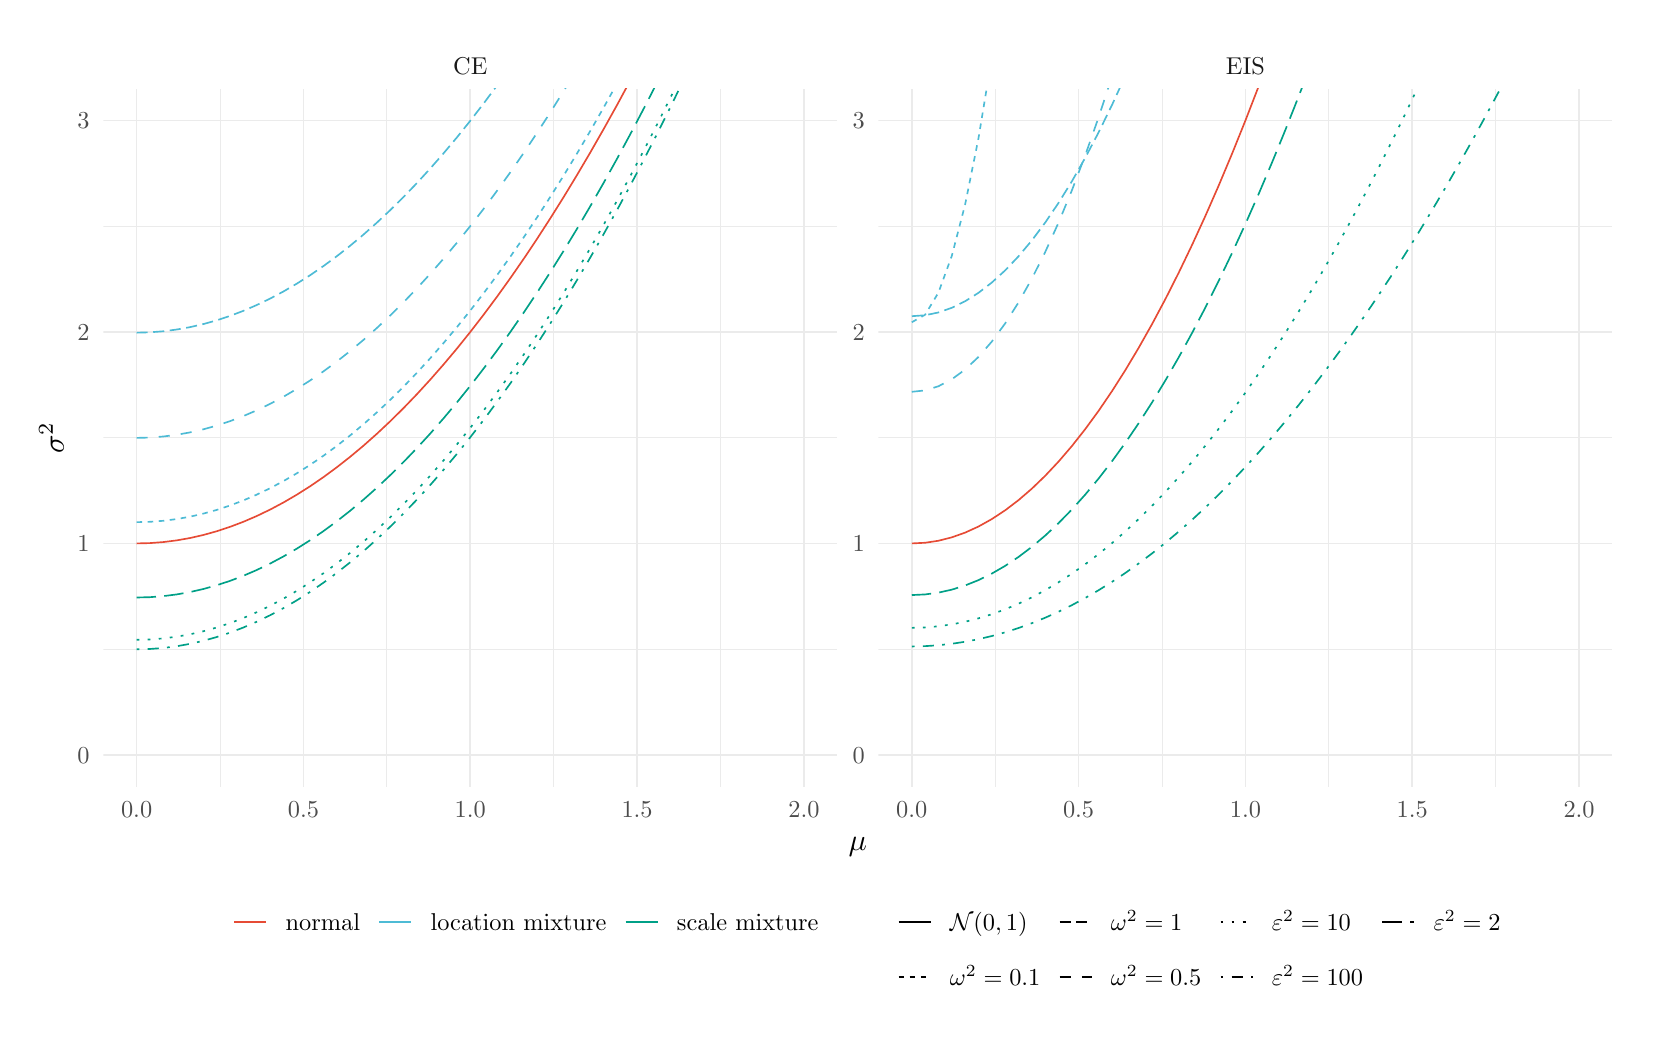
\begin{tikzpicture}[x=1pt,y=1pt]
\definecolor{fillColor}{RGB}{255,255,255}
\path[use as bounding box,fill=fillColor,fill opacity=0.00] (0,0) rectangle (578.16,361.35);
\begin{scope}
\path[clip] ( 27.31, 87.09) rectangle (292.56,339.28);
\definecolor{drawColor}{gray}{0.92}

\path[draw=drawColor,line width= 0.3pt,line join=round] ( 27.31,136.77) --
	(292.56,136.77);

\path[draw=drawColor,line width= 0.3pt,line join=round] ( 27.31,213.19) --
	(292.56,213.19);

\path[draw=drawColor,line width= 0.3pt,line join=round] ( 27.31,289.61) --
	(292.56,289.61);

\path[draw=drawColor,line width= 0.3pt,line join=round] ( 69.51, 87.09) --
	( 69.51,339.28);

\path[draw=drawColor,line width= 0.3pt,line join=round] (129.80, 87.09) --
	(129.80,339.28);

\path[draw=drawColor,line width= 0.3pt,line join=round] (190.08, 87.09) --
	(190.08,339.28);

\path[draw=drawColor,line width= 0.3pt,line join=round] (250.36, 87.09) --
	(250.36,339.28);

\path[draw=drawColor,line width= 0.6pt,line join=round] ( 27.31, 98.56) --
	(292.56, 98.56);

\path[draw=drawColor,line width= 0.6pt,line join=round] ( 27.31,174.98) --
	(292.56,174.98);

\path[draw=drawColor,line width= 0.6pt,line join=round] ( 27.31,251.40) --
	(292.56,251.40);

\path[draw=drawColor,line width= 0.6pt,line join=round] ( 27.31,327.82) --
	(292.56,327.82);

\path[draw=drawColor,line width= 0.6pt,line join=round] ( 39.37, 87.09) --
	( 39.37,339.28);

\path[draw=drawColor,line width= 0.6pt,line join=round] ( 99.65, 87.09) --
	( 99.65,339.28);

\path[draw=drawColor,line width= 0.6pt,line join=round] (159.94, 87.09) --
	(159.94,339.28);

\path[draw=drawColor,line width= 0.6pt,line join=round] (220.22, 87.09) --
	(220.22,339.28);

\path[draw=drawColor,line width= 0.6pt,line join=round] (280.51, 87.09) --
	(280.51,339.28);
\definecolor{drawColor}{RGB}{230,75,53}

\path[draw=drawColor,line width= 0.6pt,line join=round] ( 39.37,174.98) --
	( 44.19,175.10) --
	( 49.02,175.47) --
	( 53.84,176.08) --
	( 58.66,176.93) --
	( 63.48,178.03) --
	( 68.31,179.38) --
	( 73.13,180.97) --
	( 77.95,182.80) --
	( 82.77,184.88) --
	( 87.60,187.20) --
	( 92.42,189.77) --
	( 97.24,192.58) --
	(102.07,195.64) --
	(106.89,198.94) --
	(111.71,202.49) --
	(116.53,206.28) --
	(121.36,210.31) --
	(126.18,214.59) --
	(131.00,219.12) --
	(135.82,223.88) --
	(140.65,228.90) --
	(145.47,234.16) --
	(150.29,239.66) --
	(155.12,245.40) --
	(159.94,251.40) --
	(164.76,257.63) --
	(169.58,264.11) --
	(174.41,270.84) --
	(179.23,277.81) --
	(184.05,285.02) --
	(188.87,292.48) --
	(193.70,300.18) --
	(198.52,308.13) --
	(203.34,316.32) --
	(208.16,324.76) --
	(212.99,333.44) --
	(217.81,342.37) --
	(222.63,351.54) --
	(227.46,360.95) --
	(232.28,370.61) --
	(237.10,380.51) --
	(241.92,390.66) --
	(246.75,401.06) --
	(251.57,411.69) --
	(256.39,422.58) --
	(261.21,433.70) --
	(266.04,445.07) --
	(270.86,456.69) --
	(275.68,468.55) --
	(280.51,480.65);
\definecolor{drawColor}{RGB}{77,187,213}

\path[draw=drawColor,line width= 0.6pt,dash pattern=on 2pt off 2pt ,line join=round] ( 39.37,182.66) --
	( 44.19,182.79) --
	( 49.02,183.16) --
	( 53.84,183.78) --
	( 58.66,184.64) --
	( 63.48,185.75) --
	( 68.31,187.09) --
	( 73.13,188.69) --
	( 77.95,190.52) --
	( 82.77,192.61) --
	( 87.60,194.93) --
	( 92.42,197.50) --
	( 97.24,200.31) --
	(102.07,203.37) --
	(106.89,206.67) --
	(111.71,210.22) --
	(116.53,214.01) --
	(121.36,218.05) --
	(126.18,222.33) --
	(131.00,226.85) --
	(135.82,231.62) --
	(140.65,236.64) --
	(145.47,241.90) --
	(150.29,247.40) --
	(155.12,253.15) --
	(159.94,259.14) --
	(164.76,265.38) --
	(169.58,271.87) --
	(174.41,278.59) --
	(179.23,285.57) --
	(184.05,292.78) --
	(188.87,300.25) --
	(193.70,307.95) --
	(198.52,315.91) --
	(203.34,324.10) --
	(208.16,332.54) --
	(212.99,341.23) --
	(217.81,350.16) --
	(222.63,359.34) --
	(227.46,368.76) --
	(232.28,378.42) --
	(237.10,388.33) --
	(241.92,398.49) --
	(246.75,408.89) --
	(251.57,419.53) --
	(256.39,430.42) --
	(261.21,441.55) --
	(266.04,452.93) --
	(270.86,464.55) --
	(275.68,476.42) --
	(280.51,488.53);

\path[draw=drawColor,line width= 0.6pt,dash pattern=on 4pt off 2pt ,line join=round] ( 39.37,251.13) --
	( 44.19,251.27) --
	( 49.02,251.64) --
	( 53.84,252.27) --
	( 58.66,253.13) --
	( 63.48,254.24) --
	( 68.31,255.59) --
	( 73.13,257.19) --
	( 77.95,259.03) --
	( 82.77,261.12) --
	( 87.60,263.45) --
	( 92.42,266.02) --
	( 97.24,268.84) --
	(102.07,271.90) --
	(106.89,275.21) --
	(111.71,278.76) --
	(116.53,282.55) --
	(121.36,286.59) --
	(126.18,290.88) --
	(131.00,295.40) --
	(135.82,300.18) --
	(140.65,305.19) --
	(145.47,310.46) --
	(150.29,315.96) --
	(155.12,321.71) --
	(159.94,327.71) --
	(164.76,333.95) --
	(169.58,340.43) --
	(174.41,347.16) --
	(179.23,354.14) --
	(184.05,361.36) --
	(188.87,368.82) --
	(193.70,376.53) --
	(198.52,384.48) --
	(203.34,392.68) --
	(208.16,401.12) --
	(212.99,409.81) --
	(217.81,418.74) --
	(222.63,427.92) --
	(227.46,437.34) --
	(232.28,447.01) --
	(237.10,456.92) --
	(241.92,467.07) --
	(246.75,477.47) --
	(251.57,488.12) --
	(256.39,499.01) --
	(261.21,510.14) --
	(266.04,521.52) --
	(270.86,533.15) --
	(275.68,545.01) --
	(280.51,557.13);

\path[draw=drawColor,line width= 0.6pt,dash pattern=on 4pt off 4pt ,line join=round] ( 39.37,213.11) --
	( 44.19,213.24) --
	( 49.02,213.62) --
	( 53.84,214.24) --
	( 58.66,215.10) --
	( 63.48,216.21) --
	( 68.31,217.56) --
	( 73.13,219.16) --
	( 77.95,221.00) --
	( 82.77,223.08) --
	( 87.60,225.41) --
	( 92.42,227.98) --
	( 97.24,230.80) --
	(102.07,233.86) --
	(106.89,237.16) --
	(111.71,240.71) --
	(116.53,244.50) --
	(121.36,248.54) --
	(126.18,252.82) --
	(131.00,257.35) --
	(135.82,262.12) --
	(140.65,267.14) --
	(145.47,272.40) --
	(150.29,277.90) --
	(155.12,283.66) --
	(159.94,289.65) --
	(164.76,295.89) --
	(169.58,302.37) --
	(174.41,309.10) --
	(179.23,316.08) --
	(184.05,323.30) --
	(188.87,330.76) --
	(193.70,338.47) --
	(198.52,346.42) --
	(203.34,354.62) --
	(208.16,363.06) --
	(212.99,371.75) --
	(217.81,380.68) --
	(222.63,389.86) --
	(227.46,399.28) --
	(232.28,408.94) --
	(237.10,418.85) --
	(241.92,429.01) --
	(246.75,439.41) --
	(251.57,450.05) --
	(256.39,460.94) --
	(261.21,472.08) --
	(266.04,483.46) --
	(270.86,495.08) --
	(275.68,506.95) --
	(280.51,519.06);
\definecolor{drawColor}{RGB}{0,160,135}

\path[draw=drawColor,line width= 0.6pt,dash pattern=on 1pt off 3pt ,line join=round] ( 39.37,140.16) --
	( 44.19,140.29) --
	( 49.02,140.66) --
	( 53.84,141.28) --
	( 58.66,142.14) --
	( 63.48,143.24) --
	( 68.31,144.60) --
	( 73.13,146.19) --
	( 77.95,148.03) --
	( 82.77,150.12) --
	( 87.60,152.45) --
	( 92.42,155.02) --
	( 97.24,157.84) --
	(102.07,160.91) --
	(106.89,164.21) --
	(111.71,167.77) --
	(116.53,171.57) --
	(121.36,175.61) --
	(126.18,179.90) --
	(131.00,184.43) --
	(135.82,189.20) --
	(140.65,194.22) --
	(145.47,199.49) --
	(150.29,205.00) --
	(155.12,210.75) --
	(159.94,216.75) --
	(164.76,223.00) --
	(169.58,229.49) --
	(174.41,236.22) --
	(179.23,243.20) --
	(184.05,250.42) --
	(188.87,257.88) --
	(193.70,265.59) --
	(198.52,273.55) --
	(203.34,281.75) --
	(208.16,290.19) --
	(212.99,298.88) --
	(217.81,307.82) --
	(222.63,316.99) --
	(227.46,326.42) --
	(232.28,336.08) --
	(237.10,345.99) --
	(241.92,356.15) --
	(246.75,366.55) --
	(251.57,377.20) --
	(256.39,388.09) --
	(261.21,399.22) --
	(266.04,410.60) --
	(270.86,422.22) --
	(275.68,434.09) --
	(280.51,446.20);

\path[draw=drawColor,line width= 0.6pt,dash pattern=on 1pt off 3pt on 4pt off 3pt ,line join=round] ( 39.37,136.71) --
	( 44.19,136.84) --
	( 49.02,137.21) --
	( 53.84,137.83) --
	( 58.66,138.69) --
	( 63.48,139.80) --
	( 68.31,141.15) --
	( 73.13,142.75) --
	( 77.95,144.60) --
	( 82.77,146.68) --
	( 87.60,149.02) --
	( 92.42,151.59) --
	( 97.24,154.41) --
	(102.07,157.48) --
	(106.89,160.79) --
	(111.71,164.35) --
	(116.53,168.15) --
	(121.36,172.19) --
	(126.18,176.48) --
	(131.00,181.02) --
	(135.82,185.79) --
	(140.65,190.82) --
	(145.47,196.08) --
	(150.29,201.60) --
	(155.12,207.35) --
	(159.94,213.35) --
	(164.76,219.60) --
	(169.58,226.09) --
	(174.41,232.82) --
	(179.23,239.80) --
	(184.05,247.02) --
	(188.87,254.49) --
	(193.70,262.20) --
	(198.52,270.16) --
	(203.34,278.36) --
	(208.16,286.81) --
	(212.99,295.50) --
	(217.81,304.43) --
	(222.63,313.61) --
	(227.46,323.03) --
	(232.28,332.70) --
	(237.10,342.61) --
	(241.92,352.77) --
	(246.75,363.17) --
	(251.57,373.82) --
	(256.39,384.71) --
	(261.21,395.85) --
	(266.04,407.23) --
	(270.86,418.85) --
	(275.68,430.72) --
	(280.51,442.83);

\path[draw=drawColor,line width= 0.6pt,dash pattern=on 7pt off 3pt ,line join=round] ( 39.37,155.44) --
	( 44.19,155.56) --
	( 49.02,155.94) --
	( 53.84,156.55) --
	( 58.66,157.41) --
	( 63.48,158.51) --
	( 68.31,159.86) --
	( 73.13,161.45) --
	( 77.95,163.29) --
	( 82.77,165.37) --
	( 87.60,167.70) --
	( 92.42,170.27) --
	( 97.24,173.08) --
	(102.07,176.14) --
	(106.89,179.44) --
	(111.71,182.99) --
	(116.53,186.78) --
	(121.36,190.82) --
	(126.18,195.10) --
	(131.00,199.63) --
	(135.82,204.40) --
	(140.65,209.42) --
	(145.47,214.68) --
	(150.29,220.19) --
	(155.12,225.94) --
	(159.94,231.93) --
	(164.76,238.17) --
	(169.58,244.66) --
	(174.41,251.39) --
	(179.23,258.36) --
	(184.05,265.58) --
	(188.87,273.04) --
	(193.70,280.75) --
	(198.52,288.70) --
	(203.34,296.90) --
	(208.16,305.34) --
	(212.99,314.02) --
	(217.81,322.96) --
	(222.63,332.13) --
	(227.46,341.55) --
	(232.28,351.21) --
	(237.10,361.12) --
	(241.92,371.28) --
	(246.75,381.68) --
	(251.57,392.32) --
	(256.39,403.21) --
	(261.21,414.34) --
	(266.04,425.71) --
	(270.86,437.33) --
	(275.68,449.20) --
	(280.51,461.31);
\end{scope}
\begin{scope}
\path[clip] (307.41, 87.09) rectangle (572.66,339.28);
\definecolor{drawColor}{gray}{0.92}

\path[draw=drawColor,line width= 0.3pt,line join=round] (307.41,136.77) --
	(572.66,136.77);

\path[draw=drawColor,line width= 0.3pt,line join=round] (307.41,213.19) --
	(572.66,213.19);

\path[draw=drawColor,line width= 0.3pt,line join=round] (307.41,289.61) --
	(572.66,289.61);

\path[draw=drawColor,line width= 0.3pt,line join=round] (349.61, 87.09) --
	(349.61,339.28);

\path[draw=drawColor,line width= 0.3pt,line join=round] (409.89, 87.09) --
	(409.89,339.28);

\path[draw=drawColor,line width= 0.3pt,line join=round] (470.18, 87.09) --
	(470.18,339.28);

\path[draw=drawColor,line width= 0.3pt,line join=round] (530.46, 87.09) --
	(530.46,339.28);

\path[draw=drawColor,line width= 0.6pt,line join=round] (307.41, 98.56) --
	(572.66, 98.56);

\path[draw=drawColor,line width= 0.6pt,line join=round] (307.41,174.98) --
	(572.66,174.98);

\path[draw=drawColor,line width= 0.6pt,line join=round] (307.41,251.40) --
	(572.66,251.40);

\path[draw=drawColor,line width= 0.6pt,line join=round] (307.41,327.82) --
	(572.66,327.82);

\path[draw=drawColor,line width= 0.6pt,line join=round] (319.47, 87.09) --
	(319.47,339.28);

\path[draw=drawColor,line width= 0.6pt,line join=round] (379.75, 87.09) --
	(379.75,339.28);

\path[draw=drawColor,line width= 0.6pt,line join=round] (440.04, 87.09) --
	(440.04,339.28);

\path[draw=drawColor,line width= 0.6pt,line join=round] (500.32, 87.09) --
	(500.32,339.28);

\path[draw=drawColor,line width= 0.6pt,line join=round] (560.60, 87.09) --
	(560.60,339.28);
\definecolor{drawColor}{RGB}{230,75,53}

\path[draw=drawColor,line width= 0.6pt,line join=round] (319.47,174.98) --
	(324.29,175.22) --
	(329.11,175.95) --
	(333.94,177.18) --
	(338.76,178.89) --
	(343.58,181.09) --
	(348.40,183.78) --
	(353.23,186.96) --
	(358.05,190.63) --
	(362.87,194.78) --
	(367.69,199.43) --
	(372.52,204.57) --
	(377.34,210.19) --
	(382.16,216.30) --
	(386.99,222.91) --
	(391.81,230.00) --
	(396.63,237.58) --
	(401.45,245.65) --
	(406.28,254.21) --
	(411.10,263.26) --
	(415.92,272.79) --
	(420.74,282.82) --
	(425.57,293.34) --
	(430.39,304.34) --
	(435.21,315.83) --
	(440.04,327.82) --
	(444.86,340.29) --
	(449.68,353.25) --
	(454.50,366.70) --
	(459.33,380.64) --
	(464.15,395.06) --
	(468.97,409.98) --
	(473.79,425.39) --
	(478.62,441.28) --
	(483.44,457.67) --
	(488.26,474.54) --
	(493.09,491.90) --
	(497.91,509.76) --
	(502.73,528.10) --
	(507.55,546.93) --
	(512.38,566.24) --
	(517.20,586.05) --
	(522.02,606.35) --
	(526.84,627.14) --
	(531.67,648.41) --
	(536.49,670.18) --
	(541.31,692.43) --
	(546.14,715.17) --
	(550.96,738.40) --
	(555.78,762.12) --
	(560.60,786.33);
\definecolor{drawColor}{RGB}{77,187,213}

\path[draw=drawColor,line width= 0.6pt,dash pattern=on 2pt off 2pt ,line join=round] (319.47,254.90) --
	(324.29,257.62) --
	(329.11,265.62) --
	(333.94,278.91) --
	(338.76,297.51) --
	(343.58,321.43) --
	(348.40,350.70) --
	(353.23,385.32) --
	(358.05,425.30) --
	(362.87,470.66) --
	(367.69,521.41) --
	(372.52,577.55) --
	(377.34,639.10) --
	(382.16,706.06) --
	(386.99,778.45) --
	(391.81,856.27) --
	(396.63,939.53) --
	(401.45,1028.25) --
	(406.28,1122.43) --
	(411.10,1222.08) --
	(415.92,1327.22) --
	(420.74,1437.86) --
	(425.57,1554.00) --
	(430.39,1675.66) --
	(435.21,1802.84) --
	(440.04,1935.56) --
	(444.86,2073.83) --
	(449.68,2217.65) --
	(454.50,2367.05) --
	(459.33,2522.03) --
	(463.89,2673.99);

\path[draw=drawColor,line width= 0.6pt,dash pattern=on 4pt off 2pt ,line join=round] (319.47,257.09) --
	(324.29,257.43) --
	(329.11,258.44) --
	(333.94,260.13) --
	(338.76,262.50) --
	(343.58,265.54) --
	(348.40,269.26) --
	(353.23,273.66) --
	(358.05,278.74) --
	(362.87,284.49) --
	(367.69,290.93) --
	(372.52,298.06) --
	(377.34,305.86) --
	(382.16,314.36) --
	(386.99,323.53) --
	(391.81,333.39) --
	(396.63,343.94) --
	(401.45,355.18) --
	(406.28,367.10) --
	(411.10,379.71) --
	(415.92,393.00) --
	(420.74,406.99) --
	(425.57,421.66) --
	(430.39,437.02) --
	(435.21,453.06) --
	(440.04,469.80) --
	(444.86,487.22) --
	(449.68,505.33) --
	(454.50,524.12) --
	(459.33,543.61) --
	(464.15,563.78) --
	(468.97,584.64) --
	(473.79,606.19) --
	(478.62,628.42) --
	(483.44,651.34) --
	(488.26,674.95) --
	(493.09,699.25) --
	(497.91,724.23) --
	(502.73,749.90) --
	(507.55,776.26) --
	(512.38,803.31) --
	(517.20,831.04) --
	(522.02,859.46) --
	(526.84,888.57) --
	(531.67,918.36) --
	(536.49,948.84) --
	(541.31,980.01) --
	(546.14,1011.87) --
	(550.96,1044.41) --
	(555.78,1077.64) --
	(560.60,1111.56);

\path[draw=drawColor,line width= 0.6pt,dash pattern=on 4pt off 4pt ,line join=round] (319.47,229.77) --
	(324.29,230.27) --
	(329.11,231.78) --
	(333.94,234.30) --
	(338.76,237.83) --
	(343.58,242.38) --
	(348.40,247.93) --
	(353.23,254.50) --
	(358.05,262.08) --
	(362.87,270.68) --
	(367.69,280.30) --
	(372.52,290.94) --
	(377.34,302.60) --
	(382.16,315.28) --
	(386.99,328.98) --
	(391.81,343.71) --
	(396.63,359.46) --
	(401.45,376.23) --
	(406.28,394.02) --
	(411.10,412.84) --
	(415.92,432.68) --
	(420.74,453.54) --
	(425.57,475.43) --
	(430.39,498.34) --
	(435.21,522.27) --
	(440.04,547.23) --
	(444.86,573.21) --
	(449.68,600.21) --
	(454.50,628.24) --
	(459.33,657.29) --
	(464.15,687.37) --
	(468.97,718.46) --
	(473.79,750.59) --
	(478.62,783.73) --
	(483.44,817.90) --
	(488.26,853.09) --
	(493.09,889.31) --
	(497.91,926.55) --
	(502.73,964.82) --
	(507.55,1004.11) --
	(512.38,1044.42) --
	(517.20,1085.76) --
	(522.02,1128.12) --
	(526.84,1171.51) --
	(531.67,1215.92) --
	(536.49,1261.36) --
	(541.31,1307.83) --
	(546.14,1355.32) --
	(550.96,1403.83) --
	(555.78,1453.37) --
	(560.60,1503.94);
\definecolor{drawColor}{RGB}{0,160,135}

\path[draw=drawColor,line width= 0.6pt,dash pattern=on 1pt off 3pt ,line join=round] (319.47,144.47) --
	(324.29,144.62) --
	(329.11,145.04) --
	(333.94,145.73) --
	(338.76,146.68) --
	(343.58,147.91) --
	(348.40,149.40) --
	(353.23,151.17) --
	(358.05,153.21) --
	(362.87,155.51) --
	(367.69,158.09) --
	(372.52,160.95) --
	(377.34,164.07) --
	(382.16,167.47) --
	(386.99,171.14) --
	(391.81,175.08) --
	(396.63,179.30) --
	(401.45,183.79) --
	(406.28,188.55) --
	(411.10,193.58) --
	(415.92,198.89) --
	(420.74,204.47) --
	(425.57,210.32) --
	(430.39,216.44) --
	(435.21,222.83) --
	(440.04,229.49) --
	(444.86,236.43) --
	(449.68,243.63) --
	(454.50,251.10) --
	(459.33,258.84) --
	(464.15,266.85) --
	(468.97,275.13) --
	(473.79,283.68) --
	(478.62,292.50) --
	(483.44,301.58) --
	(488.26,310.93) --
	(493.09,320.55) --
	(497.91,330.43) --
	(502.73,340.58) --
	(507.55,351.00) --
	(512.38,361.68) --
	(517.20,372.63) --
	(522.02,383.84) --
	(526.84,395.32) --
	(531.67,407.06) --
	(536.49,419.07) --
	(541.31,431.34) --
	(546.14,443.88) --
	(550.96,456.68) --
	(555.78,469.74) --
	(560.60,483.07);

\path[draw=drawColor,line width= 0.6pt,dash pattern=on 1pt off 3pt on 4pt off 3pt ,line join=round] (319.47,137.75) --
	(324.29,137.87) --
	(329.11,138.19) --
	(333.94,138.72) --
	(338.76,139.45) --
	(343.58,140.38) --
	(348.40,141.52) --
	(353.23,142.86) --
	(358.05,144.42) --
	(362.87,146.17) --
	(367.69,148.14) --
	(372.52,150.31) --
	(377.34,152.69) --
	(382.16,155.28) --
	(386.99,158.08) --
	(391.81,161.09) --
	(396.63,164.30) --
	(401.45,167.73) --
	(406.28,171.36) --
	(411.10,175.20) --
	(415.92,179.25) --
	(420.74,183.51) --
	(425.57,187.98) --
	(430.39,192.65) --
	(435.21,197.53) --
	(440.04,202.62) --
	(444.86,207.92) --
	(449.68,213.42) --
	(454.50,219.13) --
	(459.33,225.05) --
	(464.15,231.17) --
	(468.97,237.50) --
	(473.79,244.03) --
	(478.62,250.77) --
	(483.44,257.72) --
	(488.26,264.87) --
	(493.09,272.22) --
	(497.91,279.78) --
	(502.73,287.54) --
	(507.55,295.51) --
	(512.38,303.68) --
	(517.20,312.05) --
	(522.02,320.63) --
	(526.84,329.41) --
	(531.67,338.40) --
	(536.49,347.58) --
	(541.31,356.97) --
	(546.14,366.56) --
	(550.96,376.36) --
	(555.78,386.35) --
	(560.60,396.55);

\path[draw=drawColor,line width= 0.6pt,dash pattern=on 7pt off 3pt ,line join=round] (319.47,156.32) --
	(324.29,156.55) --
	(329.11,157.20) --
	(333.94,158.28) --
	(338.76,159.79) --
	(343.58,161.72) --
	(348.40,164.09) --
	(353.23,166.88) --
	(358.05,170.10) --
	(362.87,173.75) --
	(367.69,177.82) --
	(372.52,182.33) --
	(377.34,187.27) --
	(382.16,192.64) --
	(386.99,198.44) --
	(391.81,204.66) --
	(396.63,211.32) --
	(401.45,218.40) --
	(406.28,225.91) --
	(411.10,233.85) --
	(415.92,242.22) --
	(420.74,251.01) --
	(425.57,260.23) --
	(430.39,269.88) --
	(435.21,279.95) --
	(440.04,290.45) --
	(444.86,301.37) --
	(449.68,312.72) --
	(454.50,324.48) --
	(459.33,336.68) --
	(464.15,349.29) --
	(468.97,362.33) --
	(473.79,375.79) --
	(478.62,389.67) --
	(483.44,403.97) --
	(488.26,418.70) --
	(493.09,433.84) --
	(497.91,449.41) --
	(502.73,465.39) --
	(507.55,481.79) --
	(512.38,498.62) --
	(517.20,515.86) --
	(522.02,533.52) --
	(526.84,551.60) --
	(531.67,570.09) --
	(536.49,589.00) --
	(541.31,608.33) --
	(546.14,628.08) --
	(550.96,648.24) --
	(555.78,668.82) --
	(560.60,689.81);
\end{scope}
\begin{scope}
\path[clip] ( 27.31,339.28) rectangle (292.56,355.85);
\definecolor{drawColor}{gray}{0.10}

\node[text=drawColor,anchor=base,inner sep=0pt, outer sep=0pt, scale=  0.88] at (159.94,344.53) {CE};
\end{scope}
\begin{scope}
\path[clip] (307.41,339.28) rectangle (572.66,355.85);
\definecolor{drawColor}{gray}{0.10}

\node[text=drawColor,anchor=base,inner sep=0pt, outer sep=0pt, scale=  0.88] at (440.04,344.53) {EIS};
\end{scope}
\begin{scope}
\path[clip] (  0.00,  0.00) rectangle (578.16,361.35);
\definecolor{drawColor}{gray}{0.30}

\node[text=drawColor,anchor=base,inner sep=0pt, outer sep=0pt, scale=  0.88] at ( 39.37, 76.08) {0.0};

\node[text=drawColor,anchor=base,inner sep=0pt, outer sep=0pt, scale=  0.88] at ( 99.65, 76.08) {0.5};

\node[text=drawColor,anchor=base,inner sep=0pt, outer sep=0pt, scale=  0.88] at (159.94, 76.08) {1.0};

\node[text=drawColor,anchor=base,inner sep=0pt, outer sep=0pt, scale=  0.88] at (220.22, 76.08) {1.5};

\node[text=drawColor,anchor=base,inner sep=0pt, outer sep=0pt, scale=  0.88] at (280.51, 76.08) {2.0};
\end{scope}
\begin{scope}
\path[clip] (  0.00,  0.00) rectangle (578.16,361.35);
\definecolor{drawColor}{gray}{0.30}

\node[text=drawColor,anchor=base,inner sep=0pt, outer sep=0pt, scale=  0.88] at (319.47, 76.08) {0.0};

\node[text=drawColor,anchor=base,inner sep=0pt, outer sep=0pt, scale=  0.88] at (379.75, 76.08) {0.5};

\node[text=drawColor,anchor=base,inner sep=0pt, outer sep=0pt, scale=  0.88] at (440.04, 76.08) {1.0};

\node[text=drawColor,anchor=base,inner sep=0pt, outer sep=0pt, scale=  0.88] at (500.32, 76.08) {1.5};

\node[text=drawColor,anchor=base,inner sep=0pt, outer sep=0pt, scale=  0.88] at (560.60, 76.08) {2.0};
\end{scope}
\begin{scope}
\path[clip] (  0.00,  0.00) rectangle (578.16,361.35);
\definecolor{drawColor}{gray}{0.30}

\node[text=drawColor,anchor=base east,inner sep=0pt, outer sep=0pt, scale=  0.88] at (302.46, 95.53) {0};

\node[text=drawColor,anchor=base east,inner sep=0pt, outer sep=0pt, scale=  0.88] at (302.46,171.95) {1};

\node[text=drawColor,anchor=base east,inner sep=0pt, outer sep=0pt, scale=  0.88] at (302.46,248.37) {2};

\node[text=drawColor,anchor=base east,inner sep=0pt, outer sep=0pt, scale=  0.88] at (302.46,324.79) {3};
\end{scope}
\begin{scope}
\path[clip] (  0.00,  0.00) rectangle (578.16,361.35);
\definecolor{drawColor}{gray}{0.30}

\node[text=drawColor,anchor=base east,inner sep=0pt, outer sep=0pt, scale=  0.88] at ( 22.36, 95.53) {0};

\node[text=drawColor,anchor=base east,inner sep=0pt, outer sep=0pt, scale=  0.88] at ( 22.36,171.95) {1};

\node[text=drawColor,anchor=base east,inner sep=0pt, outer sep=0pt, scale=  0.88] at ( 22.36,248.37) {2};

\node[text=drawColor,anchor=base east,inner sep=0pt, outer sep=0pt, scale=  0.88] at ( 22.36,324.79) {3};
\end{scope}
\begin{scope}
\path[clip] (  0.00,  0.00) rectangle (578.16,361.35);
\definecolor{drawColor}{RGB}{0,0,0}

\node[text=drawColor,anchor=base,inner sep=0pt, outer sep=0pt, scale=  1.10] at (299.99, 64.05) {$\mu$};
\end{scope}
\begin{scope}
\path[clip] (  0.00,  0.00) rectangle (578.16,361.35);
\definecolor{drawColor}{RGB}{0,0,0}

\node[text=drawColor,rotate= 90.00,anchor=base,inner sep=0pt, outer sep=0pt, scale=  1.10] at ( 13.08,213.19) {$\sigma^2$};
\end{scope}
\begin{scope}
\path[clip] (  0.00,  0.00) rectangle (578.16,361.35);
\definecolor{drawColor}{RGB}{230,75,53}

\path[draw=drawColor,line width= 0.6pt,line join=round] ( 74.73, 38.18) -- ( 86.29, 38.18);
\end{scope}
\begin{scope}
\path[clip] (  0.00,  0.00) rectangle (578.16,361.35);
\definecolor{drawColor}{RGB}{77,187,213}

\path[draw=drawColor,line width= 0.6pt,line join=round] (127.09, 38.18) -- (138.65, 38.18);
\end{scope}
\begin{scope}
\path[clip] (  0.00,  0.00) rectangle (578.16,361.35);
\definecolor{drawColor}{RGB}{0,160,135}

\path[draw=drawColor,line width= 0.6pt,line join=round] (216.11, 38.18) -- (227.67, 38.18);
\end{scope}
\begin{scope}
\path[clip] (  0.00,  0.00) rectangle (578.16,361.35);
\definecolor{drawColor}{RGB}{0,0,0}

\node[text=drawColor,anchor=base west,inner sep=0pt, outer sep=0pt, scale=  0.88] at ( 93.24, 35.15) {normal};
\end{scope}
\begin{scope}
\path[clip] (  0.00,  0.00) rectangle (578.16,361.35);
\definecolor{drawColor}{RGB}{0,0,0}

\node[text=drawColor,anchor=base west,inner sep=0pt, outer sep=0pt, scale=  0.88] at (145.60, 35.15) {location mixture};
\end{scope}
\begin{scope}
\path[clip] (  0.00,  0.00) rectangle (578.16,361.35);
\definecolor{drawColor}{RGB}{0,0,0}

\node[text=drawColor,anchor=base west,inner sep=0pt, outer sep=0pt, scale=  0.88] at (234.62, 35.15) {scale mixture};
\end{scope}
\begin{scope}
\path[clip] (  0.00,  0.00) rectangle (578.16,361.35);
\definecolor{drawColor}{RGB}{0,0,0}

\path[draw=drawColor,line width= 0.6pt,line join=round] (314.71, 38.18) -- (326.28, 38.18);
\end{scope}
\begin{scope}
\path[clip] (  0.00,  0.00) rectangle (578.16,361.35);
\definecolor{drawColor}{RGB}{0,0,0}

\path[draw=drawColor,line width= 0.6pt,dash pattern=on 2pt off 2pt ,line join=round] (314.71, 18.23) -- (326.28, 18.23);
\end{scope}
\begin{scope}
\path[clip] (  0.00,  0.00) rectangle (578.16,361.35);
\definecolor{drawColor}{RGB}{0,0,0}

\path[draw=drawColor,line width= 0.6pt,dash pattern=on 4pt off 2pt ,line join=round] (372.89, 38.18) -- (384.45, 38.18);
\end{scope}
\begin{scope}
\path[clip] (  0.00,  0.00) rectangle (578.16,361.35);
\definecolor{drawColor}{RGB}{0,0,0}

\path[draw=drawColor,line width= 0.6pt,dash pattern=on 4pt off 4pt ,line join=round] (372.89, 18.23) -- (384.45, 18.23);
\end{scope}
\begin{scope}
\path[clip] (  0.00,  0.00) rectangle (578.16,361.35);
\definecolor{drawColor}{RGB}{0,0,0}

\path[draw=drawColor,line width= 0.6pt,dash pattern=on 1pt off 3pt ,line join=round] (431.06, 38.18) -- (442.62, 38.18);
\end{scope}
\begin{scope}
\path[clip] (  0.00,  0.00) rectangle (578.16,361.35);
\definecolor{drawColor}{RGB}{0,0,0}

\path[draw=drawColor,line width= 0.6pt,dash pattern=on 1pt off 3pt on 4pt off 3pt ,line join=round] (431.06, 18.23) -- (442.62, 18.23);
\end{scope}
\begin{scope}
\path[clip] (  0.00,  0.00) rectangle (578.16,361.35);
\definecolor{drawColor}{RGB}{0,0,0}

\path[draw=drawColor,line width= 0.6pt,dash pattern=on 7pt off 3pt ,line join=round] (489.50, 38.18) -- (501.06, 38.18);
\end{scope}
\begin{scope}
\path[clip] (  0.00,  0.00) rectangle (578.16,361.35);
\definecolor{drawColor}{RGB}{0,0,0}

\node[text=drawColor,anchor=base west,inner sep=0pt, outer sep=0pt, scale=  0.88] at (333.22, 35.15) {$\mathcal N (0, 1)$};
\end{scope}
\begin{scope}
\path[clip] (  0.00,  0.00) rectangle (578.16,361.35);
\definecolor{drawColor}{RGB}{0,0,0}

\node[text=drawColor,anchor=base west,inner sep=0pt, outer sep=0pt, scale=  0.88] at (333.22, 15.20) {$\omega^2 = 0.1$};
\end{scope}
\begin{scope}
\path[clip] (  0.00,  0.00) rectangle (578.16,361.35);
\definecolor{drawColor}{RGB}{0,0,0}

\node[text=drawColor,anchor=base west,inner sep=0pt, outer sep=0pt, scale=  0.88] at (391.39, 35.15) {$\omega^2 = 1$};
\end{scope}
\begin{scope}
\path[clip] (  0.00,  0.00) rectangle (578.16,361.35);
\definecolor{drawColor}{RGB}{0,0,0}

\node[text=drawColor,anchor=base west,inner sep=0pt, outer sep=0pt, scale=  0.88] at (391.39, 15.20) {$\omega^2= 0.5$};
\end{scope}
\begin{scope}
\path[clip] (  0.00,  0.00) rectangle (578.16,361.35);
\definecolor{drawColor}{RGB}{0,0,0}

\node[text=drawColor,anchor=base west,inner sep=0pt, outer sep=0pt, scale=  0.88] at (449.57, 35.15) {$\varepsilon^2 = 10$};
\end{scope}
\begin{scope}
\path[clip] (  0.00,  0.00) rectangle (578.16,361.35);
\definecolor{drawColor}{RGB}{0,0,0}

\node[text=drawColor,anchor=base west,inner sep=0pt, outer sep=0pt, scale=  0.88] at (449.57, 15.20) {$\varepsilon^2 = 100$};
\end{scope}
\begin{scope}
\path[clip] (  0.00,  0.00) rectangle (578.16,361.35);
\definecolor{drawColor}{RGB}{0,0,0}

\node[text=drawColor,anchor=base west,inner sep=0pt, outer sep=0pt, scale=  0.88] at (508.01, 35.15) {$\varepsilon^2 = 2$};
\end{scope}
\end{tikzpicture}
%
    }
    \caption{Optimal variances $\sigma^{2}_{\ce}$ / $\sigma^{2}_\eis$ for the \acrshort{cem} (left) and \acrshort{eis} (right) as a function of the misspecified mean $\mu$. The variances produced by \acrshort{eis} tend to be larger than those produced by the \acrshort{cem}.}
    \label{fig:cem_eis_sigma2}
\end{figure}

% AREs
On the left-hand side of \Cref{fig:are} we see that for $\mu$ close to the optimal value, \aeis has smaller asymptotic variance than the \acem, except for the two bimodal location measures. Again, due to the finite sample convergence of \aeis, \Cref{prop:eis-finite-sample}, the asymptotic variance $V_{\eis}$ goes to $0$ as $\mu \to 0$. The more $\mu$ becomes misspecified, the ratio of asymptotic variances starts to grow. 

% sigma2s
In \Cref{fig:cem_eis_sigma2} we see that, except for the extreme scale mixtures, \aeis tends to produce proposals that have a larger variance than those produced by the \acem. As we will see in the discussion of \Cref{fig:rho_mu}, this might be advantageous for \aeis as proposals with a small variance run the risk of missing a large part of the probability mass of the target. 

In applications, e.g. the model studied in \Cref{cha:analysis_of_selected_models}, we are interested in the performance of the importance sampling proposals generated by the \gls{la}, \gls{cem} and \gls{eis} under more complex circumstances than those discussed in \Cref{ex:univ-gaussian-mu-fixed,ex:univ-gaussian-s2-fixed}. In particular, the dimension of $\psi$ is high ($\mathcal O(n \cdot m)$ or even $\mathcal O(n \cdot m^{2})$) and proposals may not come from a natural exponential family, so analysis based on \Cref{thm:cem-clt,thm:eis-clt} is not possible. \todo{really?} Instead, we resort to simulation studies to gain insights into the circumstances when one should prefer one method over the other.
As a leading example, we will use the following vector-autoregressive state space model with negative binomial observations. A similar, though more involved, model is studied in \Cref{sec:regional_growth_factor_model} with real data.

\begin{example}[Negative Binomial $\operatorname{VAR}(1)$ \gls{ssm}]
    \label{ex:negbinom-ar1}
    % setup 
    In this example, we consider a \gls{ssm} where states $X_{t}$ follow a stationary Gaussian $\operatorname{VAR}(1)$ process, initialized in its stationary distribution $\mathcal N(0,\Sigma)$ for \acrshort{spd} $\Sigma$. For simplicity let the transition matrices be given by a multiple of the identity, i.e. $A_{t} = \alpha I_{m}$ for all $t$ where $\alpha \in (-1, 1)$ \todo{add I to symbols}. 
    In total, the states are governed by
    \begin{align*}
    X_{0} &\sim \mathcal N(0,\Sigma) \\
    X_{t} &= \alpha X_{t - 1} + \varepsilon_{t}\\
    \varepsilon_t &\iid \mathcal N(0, (1 - \alpha^{2})\Sigma), t = 1, \dots, n
    \end{align*}
    where the $\varepsilon_{1}, \dots, n$ and $X_{0}$ are jointly independent. The observations follow a conditional negative binomial distribution 
    $$
    Y^{i}_{t} | X_{t} \sim \nbinom \left( \exp(X^{i}_{t}), r \right), \phantom{and} i = 1, \dots, p \phantom{and} t = 0, \dots, n
    $$
    and individual observations are conditionally independent given the current state. The parametrization of the negative binomial distribution $\nbinom \left( \mu, r \right)$ is such that the density is
    $$
        p_{\mu, r}(y) = \binom{y + r - 1}{r} \left( \frac{\mu}{r + \mu} \right)^{y} \left( \frac{r}{r + \mu} \right)^{r} \propto \mu^{y} (\mu + r)^{-(r + y)},
    $$
    where proportionality is in $\mu$, with expectation $\mu$, variance $\mu + \frac{\mu^{2}}{r}$ and support $\N_{0}$. 
\end{example}

%% simulation study on MSE/Bias/Variance

Our first simulation study concerns the non-asymptotic behavior of the \gls{cem} and \gls{eis} estimators, i.e. finite sample analogs of \Cref{thm:cem-clt,thm:eis-clt}. To this end,
we let $m = 1$ in \Cref{ex:negbinom-ar1} and fix $n$ to \todo{...}. 
We then simulate once from the marginal distribution of $Y$ and perform the \gls{la} to a prespecified precision $\epsilon$ and maximum number of iterations $n_{\text{iter}}$, obtaining a proposal distribution $\G_{\la}$. Using a large number of samples $N_{\text{true}}$ from this proposal we find the optimal $\G_{\ce}$ and $\G_{\eis}$ using the same desired precision and number of iterations as for the \gls{la}. For the remainder of this section, we ignore sampling variation in these proposals and treat them as exact. 

%% posterior marginal means and variances
To determine the non-asymptotic sampling behavior we now perform the above procedure again, using only $N \ll N_{\text{true}}$ many samples for both procedures, obtaining proposals $\hat\P^{N}_{\ce}$ and $\hat \P^{N}_{\eis}$. As the full proposals are Gaussian distributions on $\R^{(n+1)\times m}$, either given as the posterior of a \gls{glssm} (\gls{la}, \gls{eis}) or by a Gaussian Markov process(\gls{cem}), see \Cref{sec:gaussian_importance_sampling_for_state_space_models}. 
This procedure is repeated $M$ times for every sample size $N$ considered, with different initial random seeds, obtaining $\hat\P^{N,i}_{\ce}$ and $\hat \P^{N,i}_{\eis}$ for $i = 1, \dots, M$.

To assess the speed of convergence of the \gls{cem} and \gls{eis} we then estimate the mean squared error of means and variances of the $(n+1) \times m$ univariate marginals as $N$, the number of samples used to obtain $\hpce$ or $\hpeis$, grows. For the true value, we take the univariate means and variances of $\G_{\ce}$ and $\G_{\eis}$ respectively. Additionally, we perform a bias-variance decomposition to see where the estimation error originates. 

More concretely, fix $N$ and denote by $\mu, \sigma^{2} \in \mathbf R^{(n + 1) \cdot m}$ the marginal means and variances of $\G_{\ce}$ ($\G_{\eis}$). 
Let $\hat\mu_{i}, \hat\sigma^{2}_{i}\in\mathbf R^{(n + 1) \cdot m}$ be the marginal means and variances of $\G^{N,i}_{\ce}$ ($\G^{N,i}_{\eis}$) for $i = 1,\dots, M$. 
Now 
$$
\widehat{\text{aMSE}} = \frac{1}{M} \frac{1}{(n + 1)m} \sum_{i = 1}^M \lVert \mu - \hat\mu_{i} \rVert_{2}^2 + \lVert \sigma^{2} - \hat\sigma_{i}^2 \rVert^{2}_{2}
$$
is an estimate of the mean-squared error of $(\mu, \sigma^{2})$, where we divide by $(n+1)m$ to make estimates comparable across models of different dimensions. 

%The $\text{ASE}_{i}$ is of interest to the practitioner as they usually only run a single iteration of the optimal importance sampling procedure. So while a low $\text{AMSE}$ is desirable, the variance of $\text{ASE}$ should also be small in practice, as otherwise several runs of the optimal importance sampling procedure may be required to obtain a good proposal.

In \Cref{fig:mse_bias_var_decomposition} we show the $\widehat{\text{aMSE}}$ for both the \gls{cem} and \gls{eis} for varying values of $N$. As is evident from this Figure, the \gls{cem} consistently has a larger aMSE than \gls{eis}, for all values of $N$. Thus the \gls{cem} requires several orders of magnitude more samples to obtain the same precision as \gls{eis}.

For further investigation, we perform a bias-variance decomposition of the aMSE for both the means $\mu$ and variances $\sigma^{2}$. Consider the average means and variances over the $M$ simulations,
\begin{align*}
    \bar \mu = \frac{1}{M} \sum_{i=1}^{M} \hat\mu_{i} && \bar \sigma^{2} = \frac{1}{M} \sum_{i=1}^{M} \hat\sigma^{2}_{i},
\end{align*}
and the state-average squared bias and variance
\begin{align*}
    \text{aBias}^{2}_{\mu} &= \frac{1}{(n+1)m} \lVert \mu - \bar\mu \rVert^{2}_{2}, \\
    \text{aVar}_{\mu} &= \frac{1}{M - 1}\frac{1}{(n+1)m} \sum_{i=1}^M \lVert \bar\mu - \mu_{i} \rVert^{2}_{2},\\
    \text{aBias}^{2}_{\sigma^{2}} &= \frac{1}{(n+1)m} \lVert \sigma^{2} - \bar\sigma^{2} \rVert^{2}_{2}, \\
    \text{aVar}_{\sigma^{2}} &= \frac{1}{M - 1}\frac{1}{(n+1)m} \sum_{i=1}^M \lVert \bar\sigma^{2} - \sigma^{2}_{i} \rVert^{2}_{2}.
\end{align*}
These values are depicted in \Cref{fig:mse_bias_var_decomposition}. 
\begin{figure}
    \resizebox{\textwidth}{!}{%
        % Created by tikzDevice version 0.12.6 on 2024-05-22 14:37:09
% !TEX encoding = UTF-8 Unicode
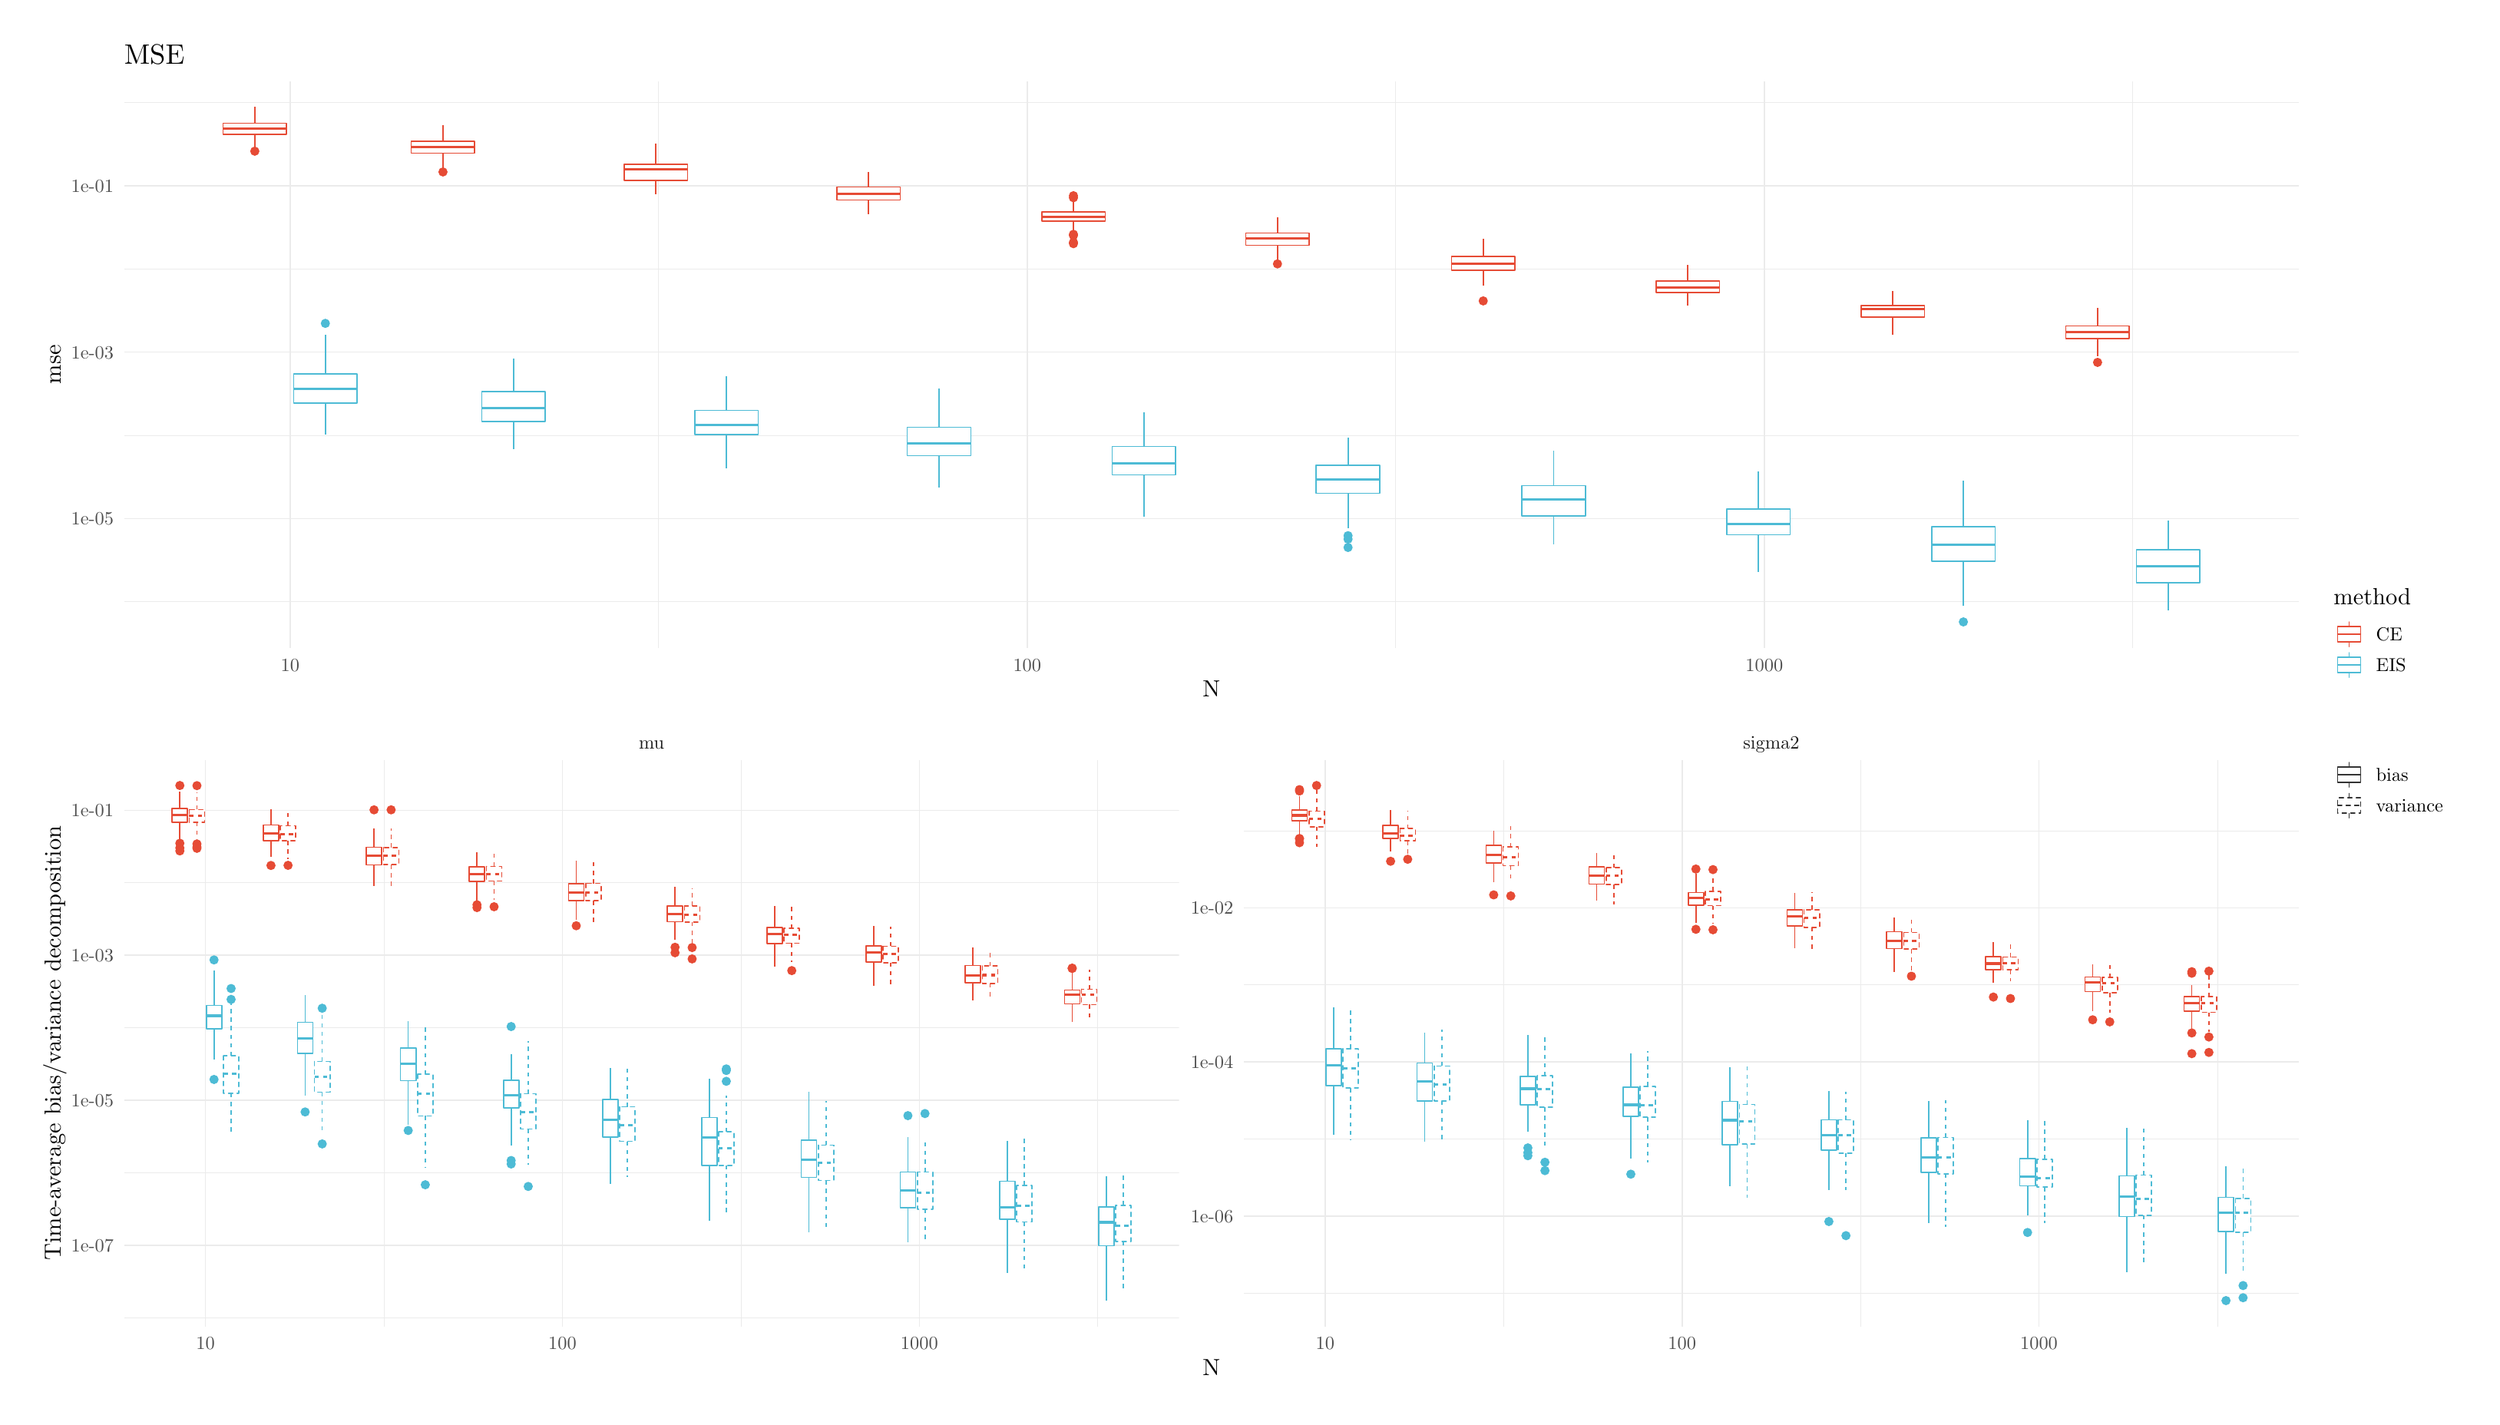
\begin{tikzpicture}[x=1pt,y=1pt]
\definecolor{fillColor}{RGB}{255,255,255}
\path[use as bounding box,fill=fillColor,fill opacity=0.00] (0,0) rectangle (1156.32,650.43);
\begin{scope}
\path[clip] ( 48.45,355.61) rectangle (1071.82,622.27);
\definecolor{drawColor}{gray}{0.92}

\path[draw=drawColor,line width= 0.3pt,line join=round] ( 48.45,377.19) --
	(1071.82,377.19);

\path[draw=drawColor,line width= 0.3pt,line join=round] ( 48.45,455.52) --
	(1071.82,455.52);

\path[draw=drawColor,line width= 0.3pt,line join=round] ( 48.45,533.86) --
	(1071.82,533.86);

\path[draw=drawColor,line width= 0.3pt,line join=round] ( 48.45,612.20) --
	(1071.82,612.20);

\path[draw=drawColor,line width= 0.3pt,line join=round] (299.97,355.61) --
	(299.97,622.27);

\path[draw=drawColor,line width= 0.3pt,line join=round] (646.87,355.61) --
	(646.87,622.27);

\path[draw=drawColor,line width= 0.3pt,line join=round] (993.77,355.61) --
	(993.77,622.27);

\path[draw=drawColor,line width= 0.6pt,line join=round] ( 48.45,416.35) --
	(1071.82,416.35);

\path[draw=drawColor,line width= 0.6pt,line join=round] ( 48.45,494.69) --
	(1071.82,494.69);

\path[draw=drawColor,line width= 0.6pt,line join=round] ( 48.45,573.03) --
	(1071.82,573.03);

\path[draw=drawColor,line width= 0.6pt,line join=round] (126.52,355.61) --
	(126.52,622.27);

\path[draw=drawColor,line width= 0.6pt,line join=round] (473.42,355.61) --
	(473.42,622.27);

\path[draw=drawColor,line width= 0.6pt,line join=round] (820.32,355.61) --
	(820.32,622.27);
\definecolor{drawColor}{RGB}{230,75,53}
\definecolor{fillColor}{RGB}{230,75,53}

\path[draw=drawColor,line width= 0.4pt,line join=round,line cap=round,fill=fillColor] (109.91,589.27) circle (  1.96);

\path[draw=drawColor,line width= 0.6pt,line join=round] (109.91,602.43) -- (109.91,610.15);

\path[draw=drawColor,line width= 0.6pt,line join=round] (109.91,597.18) -- (109.91,589.35);
\definecolor{fillColor}{RGB}{255,255,255}

\path[draw=drawColor,line width= 0.6pt,line join=round,line cap=round,fill=fillColor] ( 94.97,602.43) --
	( 94.97,597.18) --
	(124.86,597.18) --
	(124.86,602.43) --
	( 94.97,602.43) --
	cycle;

\path[draw=drawColor,line width= 1.1pt,line join=round] ( 94.97,599.88) -- (124.86,599.88);
\definecolor{fillColor}{RGB}{230,75,53}

\path[draw=drawColor,line width= 0.4pt,line join=round,line cap=round,fill=fillColor] (198.47,579.50) circle (  1.96);

\path[draw=drawColor,line width= 0.6pt,line join=round] (198.47,594.01) -- (198.47,601.62);

\path[draw=drawColor,line width= 0.6pt,line join=round] (198.47,588.28) -- (198.47,581.12);
\definecolor{fillColor}{RGB}{255,255,255}

\path[draw=drawColor,line width= 0.6pt,line join=round,line cap=round,fill=fillColor] (183.52,594.01) --
	(183.52,588.28) --
	(213.41,588.28) --
	(213.41,594.01) --
	(183.52,594.01) --
	cycle;

\path[draw=drawColor,line width= 1.1pt,line join=round] (183.52,591.17) -- (213.41,591.17);

\path[draw=drawColor,line width= 0.6pt,line join=round] (298.65,583.04) -- (298.65,592.79);

\path[draw=drawColor,line width= 0.6pt,line join=round] (298.65,575.51) -- (298.65,568.86);

\path[draw=drawColor,line width= 0.6pt,line join=round,line cap=round,fill=fillColor] (283.71,583.04) --
	(283.71,575.51) --
	(313.59,575.51) --
	(313.59,583.04) --
	(283.71,583.04) --
	cycle;

\path[draw=drawColor,line width= 1.1pt,line join=round] (283.71,580.63) -- (313.59,580.63);

\path[draw=drawColor,line width= 0.6pt,line join=round] (398.71,572.42) -- (398.71,579.51);

\path[draw=drawColor,line width= 0.6pt,line join=round] (398.71,566.26) -- (398.71,559.75);

\path[draw=drawColor,line width= 0.6pt,line join=round,line cap=round,fill=fillColor] (383.77,572.42) --
	(383.77,566.26) --
	(413.65,566.26) --
	(413.65,572.42) --
	(383.77,572.42) --
	cycle;

\path[draw=drawColor,line width= 1.1pt,line join=round] (383.77,569.10) -- (413.65,569.10);
\definecolor{fillColor}{RGB}{230,75,53}

\path[draw=drawColor,line width= 0.4pt,line join=round,line cap=round,fill=fillColor] (495.18,549.62) circle (  1.96);

\path[draw=drawColor,line width= 0.4pt,line join=round,line cap=round,fill=fillColor] (495.18,568.31) circle (  1.96);

\path[draw=drawColor,line width= 0.4pt,line join=round,line cap=round,fill=fillColor] (495.18,567.37) circle (  1.96);

\path[draw=drawColor,line width= 0.4pt,line join=round,line cap=round,fill=fillColor] (495.18,550.15) circle (  1.96);

\path[draw=drawColor,line width= 0.4pt,line join=round,line cap=round,fill=fillColor] (495.18,546.37) circle (  1.96);

\path[draw=drawColor,line width= 0.4pt,line join=round,line cap=round,fill=fillColor] (495.18,545.75) circle (  1.96);

\path[draw=drawColor,line width= 0.6pt,line join=round] (495.18,560.64) -- (495.18,566.67);

\path[draw=drawColor,line width= 0.6pt,line join=round] (495.18,556.47) -- (495.18,551.07);
\definecolor{fillColor}{RGB}{255,255,255}

\path[draw=drawColor,line width= 0.6pt,line join=round,line cap=round,fill=fillColor] (480.23,560.64) --
	(480.23,556.47) --
	(510.12,556.47) --
	(510.12,560.64) --
	(480.23,560.64) --
	cycle;

\path[draw=drawColor,line width= 1.1pt,line join=round] (480.23,558.41) -- (510.12,558.41);
\definecolor{fillColor}{RGB}{230,75,53}

\path[draw=drawColor,line width= 0.4pt,line join=round,line cap=round,fill=fillColor] (591.20,536.22) circle (  1.96);

\path[draw=drawColor,line width= 0.6pt,line join=round] (591.20,550.79) -- (591.20,558.01);

\path[draw=drawColor,line width= 0.6pt,line join=round] (591.20,545.03) -- (591.20,537.39);
\definecolor{fillColor}{RGB}{255,255,255}

\path[draw=drawColor,line width= 0.6pt,line join=round,line cap=round,fill=fillColor] (576.25,550.79) --
	(576.25,545.03) --
	(606.14,545.03) --
	(606.14,550.79) --
	(576.25,550.79) --
	cycle;

\path[draw=drawColor,line width= 1.1pt,line join=round] (576.25,548.11) -- (606.14,548.11);
\definecolor{fillColor}{RGB}{230,75,53}

\path[draw=drawColor,line width= 0.4pt,line join=round,line cap=round,fill=fillColor] (688.03,518.80) circle (  1.96);

\path[draw=drawColor,line width= 0.6pt,line join=round] (688.03,539.77) -- (688.03,548.16);

\path[draw=drawColor,line width= 0.6pt,line join=round] (688.03,533.22) -- (688.03,525.96);
\definecolor{fillColor}{RGB}{255,255,255}

\path[draw=drawColor,line width= 0.6pt,line join=round,line cap=round,fill=fillColor] (673.08,539.77) --
	(673.08,533.22) --
	(702.97,533.22) --
	(702.97,539.77) --
	(673.08,539.77) --
	cycle;

\path[draw=drawColor,line width= 1.1pt,line join=round] (673.08,536.41) -- (702.97,536.41);

\path[draw=drawColor,line width= 0.6pt,line join=round] (784.28,528.06) -- (784.28,535.76);

\path[draw=drawColor,line width= 0.6pt,line join=round] (784.28,522.86) -- (784.28,516.78);

\path[draw=drawColor,line width= 0.6pt,line join=round,line cap=round,fill=fillColor] (769.34,528.06) --
	(769.34,522.86) --
	(799.23,522.86) --
	(799.23,528.06) --
	(769.34,528.06) --
	cycle;

\path[draw=drawColor,line width= 1.1pt,line join=round] (769.34,525.06) -- (799.23,525.06);

\path[draw=drawColor,line width= 0.6pt,line join=round] (880.79,516.67) -- (880.79,523.61);

\path[draw=drawColor,line width= 0.6pt,line join=round] (880.79,511.12) -- (880.79,502.84);

\path[draw=drawColor,line width= 0.6pt,line join=round,line cap=round,fill=fillColor] (865.85,516.67) --
	(865.85,511.12) --
	(895.73,511.12) --
	(895.73,516.67) --
	(865.85,516.67) --
	cycle;

\path[draw=drawColor,line width= 1.1pt,line join=round] (865.85,514.82) -- (895.73,514.82);
\definecolor{fillColor}{RGB}{230,75,53}

\path[draw=drawColor,line width= 0.4pt,line join=round,line cap=round,fill=fillColor] (977.15,489.87) circle (  1.96);

\path[draw=drawColor,line width= 0.6pt,line join=round] (977.15,507.02) -- (977.15,515.40);

\path[draw=drawColor,line width= 0.6pt,line join=round] (977.15,501.00) -- (977.15,492.74);
\definecolor{fillColor}{RGB}{255,255,255}

\path[draw=drawColor,line width= 0.6pt,line join=round,line cap=round,fill=fillColor] (962.20,507.02) --
	(962.20,501.00) --
	(992.09,501.00) --
	(992.09,507.02) --
	(962.20,507.02) --
	cycle;

\path[draw=drawColor,line width= 1.1pt,line join=round] (962.20,504.08) -- (992.09,504.08);
\definecolor{drawColor}{RGB}{77,187,213}
\definecolor{fillColor}{RGB}{77,187,213}

\path[draw=drawColor,line width= 0.4pt,line join=round,line cap=round,fill=fillColor] (143.12,508.23) circle (  1.96);

\path[draw=drawColor,line width= 0.6pt,line join=round] (143.12,484.52) -- (143.12,502.75);

\path[draw=drawColor,line width= 0.6pt,line join=round] (143.12,470.70) -- (143.12,456.04);
\definecolor{fillColor}{RGB}{255,255,255}

\path[draw=drawColor,line width= 0.6pt,line join=round,line cap=round,fill=fillColor] (128.18,484.52) --
	(128.18,470.70) --
	(158.07,470.70) --
	(158.07,484.52) --
	(128.18,484.52) --
	cycle;

\path[draw=drawColor,line width= 1.1pt,line join=round] (128.18,477.34) -- (158.07,477.34);

\path[draw=drawColor,line width= 0.6pt,line join=round] (231.68,476.16) -- (231.68,491.74);

\path[draw=drawColor,line width= 0.6pt,line join=round] (231.68,461.96) -- (231.68,449.14);

\path[draw=drawColor,line width= 0.6pt,line join=round,line cap=round,fill=fillColor] (216.73,476.16) --
	(216.73,461.96) --
	(246.62,461.96) --
	(246.62,476.16) --
	(216.73,476.16) --
	cycle;

\path[draw=drawColor,line width= 1.1pt,line join=round] (216.73,468.25) -- (246.62,468.25);

\path[draw=drawColor,line width= 0.6pt,line join=round] (331.86,467.34) -- (331.86,483.32);

\path[draw=drawColor,line width= 0.6pt,line join=round] (331.86,455.96) -- (331.86,440.11);

\path[draw=drawColor,line width= 0.6pt,line join=round,line cap=round,fill=fillColor] (316.91,467.34) --
	(316.91,455.96) --
	(346.80,455.96) --
	(346.80,467.34) --
	(316.91,467.34) --
	cycle;

\path[draw=drawColor,line width= 1.1pt,line join=round] (316.91,460.56) -- (346.80,460.56);

\path[draw=drawColor,line width= 0.6pt,line join=round] (431.92,459.29) -- (431.92,477.47);

\path[draw=drawColor,line width= 0.6pt,line join=round] (431.92,446.02) -- (431.92,430.85);

\path[draw=drawColor,line width= 0.6pt,line join=round,line cap=round,fill=fillColor] (416.97,459.29) --
	(416.97,446.02) --
	(446.86,446.02) --
	(446.86,459.29) --
	(416.97,459.29) --
	cycle;

\path[draw=drawColor,line width= 1.1pt,line join=round] (416.97,451.75) -- (446.86,451.75);

\path[draw=drawColor,line width= 0.6pt,line join=round] (528.38,450.25) -- (528.38,466.27);

\path[draw=drawColor,line width= 0.6pt,line join=round] (528.38,436.97) -- (528.38,417.16);

\path[draw=drawColor,line width= 0.6pt,line join=round,line cap=round,fill=fillColor] (513.44,450.25) --
	(513.44,436.97) --
	(543.33,436.97) --
	(543.33,450.25) --
	(513.44,450.25) --
	cycle;

\path[draw=drawColor,line width= 1.1pt,line join=round] (513.44,442.28) -- (543.33,442.28);
\definecolor{fillColor}{RGB}{77,187,213}

\path[draw=drawColor,line width= 0.4pt,line join=round,line cap=round,fill=fillColor] (624.41,406.69) circle (  1.96);

\path[draw=drawColor,line width= 0.4pt,line join=round,line cap=round,fill=fillColor] (624.41,402.77) circle (  1.96);

\path[draw=drawColor,line width= 0.4pt,line join=round,line cap=round,fill=fillColor] (624.41,408.31) circle (  1.96);

\path[draw=drawColor,line width= 0.6pt,line join=round] (624.41,441.40) -- (624.41,454.31);

\path[draw=drawColor,line width= 0.6pt,line join=round] (624.41,428.26) -- (624.41,411.70);
\definecolor{fillColor}{RGB}{255,255,255}

\path[draw=drawColor,line width= 0.6pt,line join=round,line cap=round,fill=fillColor] (609.46,441.40) --
	(609.46,428.26) --
	(639.35,428.26) --
	(639.35,441.40) --
	(609.46,441.40) --
	cycle;

\path[draw=drawColor,line width= 1.1pt,line join=round] (609.46,434.60) -- (639.35,434.60);

\path[draw=drawColor,line width= 0.6pt,line join=round] (721.23,431.86) -- (721.23,448.33);

\path[draw=drawColor,line width= 0.6pt,line join=round] (721.23,417.63) -- (721.23,404.11);

\path[draw=drawColor,line width= 0.6pt,line join=round,line cap=round,fill=fillColor] (706.29,431.86) --
	(706.29,417.63) --
	(736.18,417.63) --
	(736.18,431.86) --
	(706.29,431.86) --
	cycle;

\path[draw=drawColor,line width= 1.1pt,line join=round] (706.29,425.20) -- (736.18,425.20);

\path[draw=drawColor,line width= 0.6pt,line join=round] (817.49,420.78) -- (817.49,438.51);

\path[draw=drawColor,line width= 0.6pt,line join=round] (817.49,408.71) -- (817.49,391.27);

\path[draw=drawColor,line width= 0.6pt,line join=round,line cap=round,fill=fillColor] (802.55,420.78) --
	(802.55,408.71) --
	(832.43,408.71) --
	(832.43,420.78) --
	(802.55,420.78) --
	cycle;

\path[draw=drawColor,line width= 1.1pt,line join=round] (802.55,413.72) -- (832.43,413.72);
\definecolor{fillColor}{RGB}{77,187,213}

\path[draw=drawColor,line width= 0.4pt,line join=round,line cap=round,fill=fillColor] (914.00,367.73) circle (  1.96);

\path[draw=drawColor,line width= 0.6pt,line join=round] (914.00,412.42) -- (914.00,434.20);

\path[draw=drawColor,line width= 0.6pt,line join=round] (914.00,396.33) -- (914.00,375.20);
\definecolor{fillColor}{RGB}{255,255,255}

\path[draw=drawColor,line width= 0.6pt,line join=round,line cap=round,fill=fillColor] (899.06,412.42) --
	(899.06,396.33) --
	(928.94,396.33) --
	(928.94,412.42) --
	(899.06,412.42) --
	cycle;

\path[draw=drawColor,line width= 1.1pt,line join=round] (899.06,404.04) -- (928.94,404.04);

\path[draw=drawColor,line width= 0.6pt,line join=round] (1010.36,401.68) -- (1010.36,415.31);

\path[draw=drawColor,line width= 0.6pt,line join=round] (1010.36,386.17) -- (1010.36,373.01);

\path[draw=drawColor,line width= 0.6pt,line join=round,line cap=round,fill=fillColor] (995.41,401.68) --
	(995.41,386.17) --
	(1025.30,386.17) --
	(1025.30,401.68) --
	(995.41,401.68) --
	cycle;

\path[draw=drawColor,line width= 1.1pt,line join=round] (995.41,393.86) -- (1025.30,393.86);
\end{scope}
\begin{scope}
\path[clip] (  0.00,  0.00) rectangle (1156.32,650.43);
\definecolor{drawColor}{gray}{0.30}

\node[text=drawColor,anchor=base east,inner sep=0pt, outer sep=0pt, scale=  0.88] at ( 43.50,413.32) {1e-05};

\node[text=drawColor,anchor=base east,inner sep=0pt, outer sep=0pt, scale=  0.88] at ( 43.50,491.66) {1e-03};

\node[text=drawColor,anchor=base east,inner sep=0pt, outer sep=0pt, scale=  0.88] at ( 43.50,570.00) {1e-01};
\end{scope}
\begin{scope}
\path[clip] (  0.00,  0.00) rectangle (1156.32,650.43);
\definecolor{drawColor}{gray}{0.30}

\node[text=drawColor,anchor=base,inner sep=0pt, outer sep=0pt, scale=  0.88] at (126.52,344.60) {10};

\node[text=drawColor,anchor=base,inner sep=0pt, outer sep=0pt, scale=  0.88] at (473.42,344.60) {100};

\node[text=drawColor,anchor=base,inner sep=0pt, outer sep=0pt, scale=  0.88] at (820.32,344.60) {1000};
\end{scope}
\begin{scope}
\path[clip] (  0.00,  0.00) rectangle (1156.32,650.43);
\definecolor{drawColor}{RGB}{0,0,0}

\node[text=drawColor,anchor=base,inner sep=0pt, outer sep=0pt, scale=  1.10] at (560.13,332.56) {N};
\end{scope}
\begin{scope}
\path[clip] (  0.00,  0.00) rectangle (1156.32,650.43);
\definecolor{drawColor}{RGB}{0,0,0}

\node[text=drawColor,rotate= 90.00,anchor=base,inner sep=0pt, outer sep=0pt, scale=  1.10] at ( 18.58,488.94) {mse};
\end{scope}
\begin{scope}
\path[clip] (  0.00,  0.00) rectangle (1156.32,650.43);
\definecolor{drawColor}{RGB}{0,0,0}

\node[text=drawColor,anchor=base west,inner sep=0pt, outer sep=0pt, scale=  1.32] at ( 48.45,630.34) {MSE};
\end{scope}
\begin{scope}
\path[clip] ( 48.45, 36.19) rectangle (544.89,302.85);
\definecolor{drawColor}{gray}{0.92}

\path[draw=drawColor,line width= 0.3pt,line join=round] ( 48.45, 40.21) --
	(544.89, 40.21);

\path[draw=drawColor,line width= 0.3pt,line join=round] ( 48.45,108.45) --
	(544.89,108.45);

\path[draw=drawColor,line width= 0.3pt,line join=round] ( 48.45,176.68) --
	(544.89,176.68);

\path[draw=drawColor,line width= 0.3pt,line join=round] ( 48.45,244.91) --
	(544.89,244.91);

\path[draw=drawColor,line width= 0.3pt,line join=round] (170.69, 36.19) --
	(170.69,302.85);

\path[draw=drawColor,line width= 0.3pt,line join=round] (338.67, 36.19) --
	(338.67,302.85);

\path[draw=drawColor,line width= 0.3pt,line join=round] (506.65, 36.19) --
	(506.65,302.85);

\path[draw=drawColor,line width= 0.6pt,line join=round] ( 48.45, 74.33) --
	(544.89, 74.33);

\path[draw=drawColor,line width= 0.6pt,line join=round] ( 48.45,142.56) --
	(544.89,142.56);

\path[draw=drawColor,line width= 0.6pt,line join=round] ( 48.45,210.80) --
	(544.89,210.80);

\path[draw=drawColor,line width= 0.6pt,line join=round] ( 48.45,279.03) --
	(544.89,279.03);

\path[draw=drawColor,line width= 0.6pt,line join=round] ( 86.70, 36.19) --
	( 86.70,302.85);

\path[draw=drawColor,line width= 0.6pt,line join=round] (254.68, 36.19) --
	(254.68,302.85);

\path[draw=drawColor,line width= 0.6pt,line join=round] (422.66, 36.19) --
	(422.66,302.85);
\definecolor{drawColor}{RGB}{230,75,53}
\definecolor{fillColor}{RGB}{230,75,53}

\path[draw=drawColor,line width= 0.4pt,line join=round,line cap=round,fill=fillColor] ( 74.64,290.73) circle (  1.96);

\path[draw=drawColor,line width= 0.4pt,line join=round,line cap=round,fill=fillColor] ( 74.64,259.94) circle (  1.96);

\path[draw=drawColor,line width= 0.4pt,line join=round,line cap=round,fill=fillColor] ( 74.64,263.55) circle (  1.96);

\path[draw=drawColor,line width= 0.4pt,line join=round,line cap=round,fill=fillColor] ( 74.64,261.36) circle (  1.96);

\path[draw=drawColor,line width= 0.6pt,line join=round] ( 74.64,279.83) -- ( 74.64,287.94);

\path[draw=drawColor,line width= 0.6pt,line join=round] ( 74.64,273.38) -- ( 74.64,263.91);
\definecolor{fillColor}{RGB}{255,255,255}

\path[draw=drawColor,line width= 0.6pt,line join=round,line cap=round,fill=fillColor] ( 71.02,279.83) --
	( 71.02,273.38) --
	( 78.26,273.38) --
	( 78.26,279.83) --
	( 71.02,279.83) --
	cycle;

\path[draw=drawColor,line width= 1.1pt,line join=round] ( 71.02,276.71) -- ( 78.26,276.71);
\definecolor{fillColor}{RGB}{230,75,53}

\path[draw=drawColor,line width= 0.4pt,line join=round,line cap=round,fill=fillColor] (117.52,253.10) circle (  1.96);

\path[draw=drawColor,line width= 0.6pt,line join=round] (117.52,272.15) -- (117.52,279.49);

\path[draw=drawColor,line width= 0.6pt,line join=round] (117.52,264.84) -- (117.52,257.32);
\definecolor{fillColor}{RGB}{255,255,255}

\path[draw=drawColor,line width= 0.6pt,line join=round,line cap=round,fill=fillColor] (113.90,272.15) --
	(113.90,264.84) --
	(121.14,264.84) --
	(121.14,272.15) --
	(113.90,272.15) --
	cycle;

\path[draw=drawColor,line width= 1.1pt,line join=round] (113.90,268.24) -- (121.14,268.24);
\definecolor{fillColor}{RGB}{230,75,53}

\path[draw=drawColor,line width= 0.4pt,line join=round,line cap=round,fill=fillColor] (166.03,279.27) circle (  1.96);

\path[draw=drawColor,line width= 0.6pt,line join=round] (166.03,261.68) -- (166.03,270.67);

\path[draw=drawColor,line width= 0.6pt,line join=round] (166.03,253.36) -- (166.03,243.56);
\definecolor{fillColor}{RGB}{255,255,255}

\path[draw=drawColor,line width= 0.6pt,line join=round,line cap=round,fill=fillColor] (162.41,261.68) --
	(162.41,253.36) --
	(169.65,253.36) --
	(169.65,261.68) --
	(162.41,261.68) --
	cycle;

\path[draw=drawColor,line width= 1.1pt,line join=round] (162.41,257.83) -- (169.65,257.83);
\definecolor{fillColor}{RGB}{230,75,53}

\path[draw=drawColor,line width= 0.4pt,line join=round,line cap=round,fill=fillColor] (214.48,233.28) circle (  1.96);

\path[draw=drawColor,line width= 0.4pt,line join=round,line cap=round,fill=fillColor] (214.48,234.60) circle (  1.96);

\path[draw=drawColor,line width= 0.6pt,line join=round] (214.48,252.45) -- (214.48,259.19);

\path[draw=drawColor,line width= 0.6pt,line join=round] (214.48,245.50) -- (214.48,236.52);
\definecolor{fillColor}{RGB}{255,255,255}

\path[draw=drawColor,line width= 0.6pt,line join=round,line cap=round,fill=fillColor] (210.87,252.45) --
	(210.87,245.50) --
	(218.10,245.50) --
	(218.10,252.45) --
	(210.87,252.45) --
	cycle;

\path[draw=drawColor,line width= 1.1pt,line join=round] (210.87,248.89) -- (218.10,248.89);
\definecolor{fillColor}{RGB}{230,75,53}

\path[draw=drawColor,line width= 0.4pt,line join=round,line cap=round,fill=fillColor] (261.20,224.72) circle (  1.96);

\path[draw=drawColor,line width= 0.6pt,line join=round] (261.20,244.46) -- (261.20,255.34);

\path[draw=drawColor,line width= 0.6pt,line join=round] (261.20,236.68) -- (261.20,227.57);
\definecolor{fillColor}{RGB}{255,255,255}

\path[draw=drawColor,line width= 0.6pt,line join=round,line cap=round,fill=fillColor] (257.58,244.46) --
	(257.58,236.68) --
	(264.81,236.68) --
	(264.81,244.46) --
	(257.58,244.46) --
	cycle;

\path[draw=drawColor,line width= 1.1pt,line join=round] (257.58,240.28) -- (264.81,240.28);
\definecolor{fillColor}{RGB}{230,75,53}

\path[draw=drawColor,line width= 0.4pt,line join=round,line cap=round,fill=fillColor] (307.69,212.03) circle (  1.96);

\path[draw=drawColor,line width= 0.4pt,line join=round,line cap=round,fill=fillColor] (307.69,214.60) circle (  1.96);

\path[draw=drawColor,line width= 0.6pt,line join=round] (307.69,234.13) -- (307.69,242.93);

\path[draw=drawColor,line width= 0.6pt,line join=round] (307.69,226.67) -- (307.69,218.03);
\definecolor{fillColor}{RGB}{255,255,255}

\path[draw=drawColor,line width= 0.6pt,line join=round,line cap=round,fill=fillColor] (304.08,234.13) --
	(304.08,226.67) --
	(311.31,226.67) --
	(311.31,234.13) --
	(304.08,234.13) --
	cycle;

\path[draw=drawColor,line width= 1.1pt,line join=round] (304.08,230.28) -- (311.31,230.28);

\path[draw=drawColor,line width= 0.6pt,line join=round] (354.58,223.99) -- (354.58,233.89);

\path[draw=drawColor,line width= 0.6pt,line join=round] (354.58,216.38) -- (354.58,205.43);

\path[draw=drawColor,line width= 0.6pt,line join=round,line cap=round,fill=fillColor] (350.96,223.99) --
	(350.96,216.38) --
	(358.20,216.38) --
	(358.20,223.99) --
	(350.96,223.99) --
	cycle;

\path[draw=drawColor,line width= 1.1pt,line join=round] (350.96,220.73) -- (358.20,220.73);

\path[draw=drawColor,line width= 0.6pt,line join=round] (401.19,215.33) -- (401.19,224.51);

\path[draw=drawColor,line width= 0.6pt,line join=round] (401.19,207.61) -- (401.19,196.40);

\path[draw=drawColor,line width= 0.6pt,line join=round,line cap=round,fill=fillColor] (397.57,215.33) --
	(397.57,207.61) --
	(404.81,207.61) --
	(404.81,215.33) --
	(397.57,215.33) --
	cycle;

\path[draw=drawColor,line width= 1.1pt,line join=round] (397.57,212.04) -- (404.81,212.04);

\path[draw=drawColor,line width= 0.6pt,line join=round] (447.93,206.05) -- (447.93,214.43);

\path[draw=drawColor,line width= 0.6pt,line join=round] (447.93,198.01) -- (447.93,189.49);

\path[draw=drawColor,line width= 0.6pt,line join=round,line cap=round,fill=fillColor] (444.31,206.05) --
	(444.31,198.01) --
	(451.54,198.01) --
	(451.54,206.05) --
	(444.31,206.05) --
	cycle;

\path[draw=drawColor,line width= 1.1pt,line join=round] (444.31,201.25) -- (451.54,201.25);
\definecolor{fillColor}{RGB}{230,75,53}

\path[draw=drawColor,line width= 0.4pt,line join=round,line cap=round,fill=fillColor] (494.59,204.79) circle (  1.96);

\path[draw=drawColor,line width= 0.4pt,line join=round,line cap=round,fill=fillColor] (494.59,204.64) circle (  1.96);

\path[draw=drawColor,line width= 0.6pt,line join=round] (494.59,194.44) -- (494.59,203.20);

\path[draw=drawColor,line width= 0.6pt,line join=round] (494.59,188.00) -- (494.59,179.61);
\definecolor{fillColor}{RGB}{255,255,255}

\path[draw=drawColor,line width= 0.6pt,line join=round,line cap=round,fill=fillColor] (490.97,194.44) --
	(490.97,188.00) --
	(498.20,188.00) --
	(498.20,194.44) --
	(490.97,194.44) --
	cycle;

\path[draw=drawColor,line width= 1.1pt,line join=round] (490.97,192.28) -- (498.20,192.28);
\definecolor{fillColor}{RGB}{230,75,53}

\path[draw=drawColor,line width= 0.4pt,line join=round,line cap=round,fill=fillColor] ( 82.68,290.67) circle (  1.96);

\path[draw=drawColor,line width= 0.4pt,line join=round,line cap=round,fill=fillColor] ( 82.68,261.17) circle (  1.96);

\path[draw=drawColor,line width= 0.4pt,line join=round,line cap=round,fill=fillColor] ( 82.68,263.24) circle (  1.96);

\path[draw=drawColor,line width= 0.4pt,line join=round,line cap=round,fill=fillColor] ( 82.68,261.78) circle (  1.96);

\path[draw=drawColor,line width= 0.6pt,dash pattern=on 2pt off 2pt ,line join=round] ( 82.68,279.43) -- ( 82.68,287.44);

\path[draw=drawColor,line width= 0.6pt,dash pattern=on 2pt off 2pt ,line join=round] ( 82.68,273.46) -- ( 82.68,264.54);
\definecolor{fillColor}{RGB}{255,255,255}

\path[draw=drawColor,line width= 0.6pt,dash pattern=on 2pt off 2pt ,line join=round,line cap=round,fill=fillColor] ( 79.06,279.43) --
	( 79.06,273.46) --
	( 86.30,273.46) --
	( 86.30,279.43) --
	( 79.06,279.43) --
	cycle;

\path[draw=drawColor,line width= 1.1pt,dash pattern=on 2pt off 2pt ,line join=round] ( 79.06,276.46) -- ( 86.30,276.46);
\definecolor{fillColor}{RGB}{230,75,53}

\path[draw=drawColor,line width= 0.4pt,line join=round,line cap=round,fill=fillColor] (125.56,253.16) circle (  1.96);

\path[draw=drawColor,line width= 0.6pt,dash pattern=on 2pt off 2pt ,line join=round] (125.56,271.80) -- (125.56,279.39);

\path[draw=drawColor,line width= 0.6pt,dash pattern=on 2pt off 2pt ,line join=round] (125.56,264.71) -- (125.56,256.05);
\definecolor{fillColor}{RGB}{255,255,255}

\path[draw=drawColor,line width= 0.6pt,dash pattern=on 2pt off 2pt ,line join=round,line cap=round,fill=fillColor] (121.94,271.80) --
	(121.94,264.71) --
	(129.18,264.71) --
	(129.18,271.80) --
	(121.94,271.80) --
	cycle;

\path[draw=drawColor,line width= 1.1pt,dash pattern=on 2pt off 2pt ,line join=round] (121.94,267.87) -- (129.18,267.87);
\definecolor{fillColor}{RGB}{230,75,53}

\path[draw=drawColor,line width= 0.4pt,line join=round,line cap=round,fill=fillColor] (174.07,279.28) circle (  1.96);

\path[draw=drawColor,line width= 0.6pt,dash pattern=on 2pt off 2pt ,line join=round] (174.07,261.55) -- (174.07,270.46);

\path[draw=drawColor,line width= 0.6pt,dash pattern=on 2pt off 2pt ,line join=round] (174.07,253.52) -- (174.07,242.85);
\definecolor{fillColor}{RGB}{255,255,255}

\path[draw=drawColor,line width= 0.6pt,dash pattern=on 2pt off 2pt ,line join=round,line cap=round,fill=fillColor] (170.45,261.55) --
	(170.45,253.52) --
	(177.69,253.52) --
	(177.69,261.55) --
	(170.45,261.55) --
	cycle;

\path[draw=drawColor,line width= 1.1pt,dash pattern=on 2pt off 2pt ,line join=round] (170.45,257.64) -- (177.69,257.64);
\definecolor{fillColor}{RGB}{230,75,53}

\path[draw=drawColor,line width= 0.4pt,line join=round,line cap=round,fill=fillColor] (222.52,233.68) circle (  1.96);

\path[draw=drawColor,line width= 0.6pt,dash pattern=on 2pt off 2pt ,line join=round] (222.52,252.64) -- (222.52,259.52);

\path[draw=drawColor,line width= 0.6pt,dash pattern=on 2pt off 2pt ,line join=round] (222.52,245.82) -- (222.52,236.94);
\definecolor{fillColor}{RGB}{255,255,255}

\path[draw=drawColor,line width= 0.6pt,dash pattern=on 2pt off 2pt ,line join=round,line cap=round,fill=fillColor] (218.91,252.64) --
	(218.91,245.82) --
	(226.14,245.82) --
	(226.14,252.64) --
	(218.91,252.64) --
	cycle;

\path[draw=drawColor,line width= 1.1pt,dash pattern=on 2pt off 2pt ,line join=round] (218.91,249.03) -- (226.14,249.03);

\path[draw=drawColor,line width= 0.6pt,dash pattern=on 2pt off 2pt ,line join=round] (269.24,244.65) -- (269.24,254.67);

\path[draw=drawColor,line width= 0.6pt,dash pattern=on 2pt off 2pt ,line join=round] (269.24,236.54) -- (269.24,224.63);

\path[draw=drawColor,line width= 0.6pt,dash pattern=on 2pt off 2pt ,line join=round,line cap=round,fill=fillColor] (265.62,244.65) --
	(265.62,236.54) --
	(272.85,236.54) --
	(272.85,244.65) --
	(265.62,244.65) --
	cycle;

\path[draw=drawColor,line width= 1.1pt,dash pattern=on 2pt off 2pt ,line join=round] (265.62,240.48) -- (272.85,240.48);
\definecolor{fillColor}{RGB}{230,75,53}

\path[draw=drawColor,line width= 0.4pt,line join=round,line cap=round,fill=fillColor] (315.73,209.12) circle (  1.96);

\path[draw=drawColor,line width= 0.4pt,line join=round,line cap=round,fill=fillColor] (315.73,214.46) circle (  1.96);

\path[draw=drawColor,line width= 0.6pt,dash pattern=on 2pt off 2pt ,line join=round] (315.73,234.15) -- (315.73,242.43);

\path[draw=drawColor,line width= 0.6pt,dash pattern=on 2pt off 2pt ,line join=round] (315.73,226.47) -- (315.73,216.36);
\definecolor{fillColor}{RGB}{255,255,255}

\path[draw=drawColor,line width= 0.6pt,dash pattern=on 2pt off 2pt ,line join=round,line cap=round,fill=fillColor] (312.12,234.15) --
	(312.12,226.47) --
	(319.35,226.47) --
	(319.35,234.15) --
	(312.12,234.15) --
	cycle;

\path[draw=drawColor,line width= 1.1pt,dash pattern=on 2pt off 2pt ,line join=round] (312.12,229.92) -- (319.35,229.92);
\definecolor{fillColor}{RGB}{230,75,53}

\path[draw=drawColor,line width= 0.4pt,line join=round,line cap=round,fill=fillColor] (362.62,203.62) circle (  1.96);

\path[draw=drawColor,line width= 0.6pt,dash pattern=on 2pt off 2pt ,line join=round] (362.62,223.51) -- (362.62,233.83);

\path[draw=drawColor,line width= 0.6pt,dash pattern=on 2pt off 2pt ,line join=round] (362.62,216.53) -- (362.62,207.74);
\definecolor{fillColor}{RGB}{255,255,255}

\path[draw=drawColor,line width= 0.6pt,dash pattern=on 2pt off 2pt ,line join=round,line cap=round,fill=fillColor] (359.00,223.51) --
	(359.00,216.53) --
	(366.24,216.53) --
	(366.24,223.51) --
	(359.00,223.51) --
	cycle;

\path[draw=drawColor,line width= 1.1pt,dash pattern=on 2pt off 2pt ,line join=round] (359.00,220.65) -- (366.24,220.65);

\path[draw=drawColor,line width= 0.6pt,dash pattern=on 2pt off 2pt ,line join=round] (409.23,215.08) -- (409.23,224.39);

\path[draw=drawColor,line width= 0.6pt,dash pattern=on 2pt off 2pt ,line join=round] (409.23,207.35) -- (409.23,196.83);

\path[draw=drawColor,line width= 0.6pt,dash pattern=on 2pt off 2pt ,line join=round,line cap=round,fill=fillColor] (405.61,215.08) --
	(405.61,207.35) --
	(412.85,207.35) --
	(412.85,215.08) --
	(405.61,215.08) --
	cycle;

\path[draw=drawColor,line width= 1.1pt,dash pattern=on 2pt off 2pt ,line join=round] (405.61,211.62) -- (412.85,211.62);

\path[draw=drawColor,line width= 0.6pt,dash pattern=on 2pt off 2pt ,line join=round] (455.97,205.82) -- (455.97,213.74);

\path[draw=drawColor,line width= 0.6pt,dash pattern=on 2pt off 2pt ,line join=round] (455.97,197.57) -- (455.97,190.82);

\path[draw=drawColor,line width= 0.6pt,dash pattern=on 2pt off 2pt ,line join=round,line cap=round,fill=fillColor] (452.35,205.82) --
	(452.35,197.57) --
	(459.58,197.57) --
	(459.58,205.82) --
	(452.35,205.82) --
	cycle;

\path[draw=drawColor,line width= 1.1pt,dash pattern=on 2pt off 2pt ,line join=round] (452.35,201.51) -- (459.58,201.51);

\path[draw=drawColor,line width= 0.6pt,dash pattern=on 2pt off 2pt ,line join=round] (502.63,194.87) -- (502.63,204.15);

\path[draw=drawColor,line width= 0.6pt,dash pattern=on 2pt off 2pt ,line join=round] (502.63,187.61) -- (502.63,179.99);

\path[draw=drawColor,line width= 0.6pt,dash pattern=on 2pt off 2pt ,line join=round,line cap=round,fill=fillColor] (499.01,194.87) --
	(499.01,187.61) --
	(506.24,187.61) --
	(506.24,194.87) --
	(499.01,194.87) --
	cycle;

\path[draw=drawColor,line width= 1.1pt,dash pattern=on 2pt off 2pt ,line join=round] (499.01,192.34) -- (506.24,192.34);
\definecolor{drawColor}{RGB}{77,187,213}
\definecolor{fillColor}{RGB}{77,187,213}

\path[draw=drawColor,line width= 0.4pt,line join=round,line cap=round,fill=fillColor] ( 90.72,152.39) circle (  1.96);

\path[draw=drawColor,line width= 0.4pt,line join=round,line cap=round,fill=fillColor] ( 90.72,208.65) circle (  1.96);

\path[draw=drawColor,line width= 0.6pt,line join=round] ( 90.72,187.19) -- ( 90.72,203.53);

\path[draw=drawColor,line width= 0.6pt,line join=round] ( 90.72,176.20) -- ( 90.72,161.70);
\definecolor{fillColor}{RGB}{255,255,255}

\path[draw=drawColor,line width= 0.6pt,line join=round,line cap=round,fill=fillColor] ( 87.10,187.19) --
	( 87.10,176.20) --
	( 94.34,176.20) --
	( 94.34,187.19) --
	( 87.10,187.19) --
	cycle;

\path[draw=drawColor,line width= 1.1pt,line join=round] ( 87.10,182.36) -- ( 94.34,182.36);
\definecolor{fillColor}{RGB}{77,187,213}

\path[draw=drawColor,line width= 0.4pt,line join=round,line cap=round,fill=fillColor] (133.60,137.10) circle (  1.96);

\path[draw=drawColor,line width= 0.6pt,line join=round] (133.60,179.25) -- (133.60,192.09);

\path[draw=drawColor,line width= 0.6pt,line join=round] (133.60,164.68) -- (133.60,144.66);
\definecolor{fillColor}{RGB}{255,255,255}

\path[draw=drawColor,line width= 0.6pt,line join=round,line cap=round,fill=fillColor] (129.98,179.25) --
	(129.98,164.68) --
	(137.22,164.68) --
	(137.22,179.25) --
	(129.98,179.25) --
	cycle;

\path[draw=drawColor,line width= 1.1pt,line join=round] (129.98,171.68) -- (137.22,171.68);
\definecolor{fillColor}{RGB}{77,187,213}

\path[draw=drawColor,line width= 0.4pt,line join=round,line cap=round,fill=fillColor] (182.11,128.38) circle (  1.96);

\path[draw=drawColor,line width= 0.6pt,line join=round] (182.11,167.23) -- (182.11,179.78);

\path[draw=drawColor,line width= 0.6pt,line join=round] (182.11,151.86) -- (182.11,131.17);
\definecolor{fillColor}{RGB}{255,255,255}

\path[draw=drawColor,line width= 0.6pt,line join=round,line cap=round,fill=fillColor] (178.49,167.23) --
	(178.49,151.86) --
	(185.73,151.86) --
	(185.73,167.23) --
	(178.49,167.23) --
	cycle;

\path[draw=drawColor,line width= 1.1pt,line join=round] (178.49,159.66) -- (185.73,159.66);
\definecolor{fillColor}{RGB}{77,187,213}

\path[draw=drawColor,line width= 0.4pt,line join=round,line cap=round,fill=fillColor] (230.56,114.25) circle (  1.96);

\path[draw=drawColor,line width= 0.4pt,line join=round,line cap=round,fill=fillColor] (230.56,177.29) circle (  1.96);

\path[draw=drawColor,line width= 0.4pt,line join=round,line cap=round,fill=fillColor] (230.56,112.60) circle (  1.96);

\path[draw=drawColor,line width= 0.6pt,line join=round] (230.56,152.00) -- (230.56,164.22);

\path[draw=drawColor,line width= 0.6pt,line join=round] (230.56,138.95) -- (230.56,121.16);
\definecolor{fillColor}{RGB}{255,255,255}

\path[draw=drawColor,line width= 0.6pt,line join=round,line cap=round,fill=fillColor] (226.95,152.00) --
	(226.95,138.95) --
	(234.18,138.95) --
	(234.18,152.00) --
	(226.95,152.00) --
	cycle;

\path[draw=drawColor,line width= 1.1pt,line join=round] (226.95,144.86) -- (234.18,144.86);

\path[draw=drawColor,line width= 0.6pt,line join=round] (277.28,142.93) -- (277.28,157.92);

\path[draw=drawColor,line width= 0.6pt,line join=round] (277.28,125.29) -- (277.28,103.34);

\path[draw=drawColor,line width= 0.6pt,line join=round,line cap=round,fill=fillColor] (273.66,142.93) --
	(273.66,125.29) --
	(280.90,125.29) --
	(280.90,142.93) --
	(273.66,142.93) --
	cycle;

\path[draw=drawColor,line width= 1.1pt,line join=round] (273.66,133.57) -- (280.90,133.57);

\path[draw=drawColor,line width= 0.6pt,line join=round] (323.77,134.43) -- (323.77,152.66);

\path[draw=drawColor,line width= 0.6pt,line join=round] (323.77,111.92) -- (323.77, 85.88);

\path[draw=drawColor,line width= 0.6pt,line join=round,line cap=round,fill=fillColor] (320.16,134.43) --
	(320.16,111.92) --
	(327.39,111.92) --
	(327.39,134.43) --
	(320.16,134.43) --
	cycle;

\path[draw=drawColor,line width= 1.1pt,line join=round] (320.16,125.21) -- (327.39,125.21);

\path[draw=drawColor,line width= 0.6pt,line join=round] (370.66,123.90) -- (370.66,146.49);

\path[draw=drawColor,line width= 0.6pt,line join=round] (370.66,106.33) -- (370.66, 80.55);

\path[draw=drawColor,line width= 0.6pt,line join=round,line cap=round,fill=fillColor] (367.04,123.90) --
	(367.04,106.33) --
	(374.28,106.33) --
	(374.28,123.90) --
	(367.04,123.90) --
	cycle;

\path[draw=drawColor,line width= 1.1pt,line join=round] (367.04,114.72) -- (374.28,114.72);
\definecolor{fillColor}{RGB}{77,187,213}

\path[draw=drawColor,line width= 0.4pt,line join=round,line cap=round,fill=fillColor] (417.27,135.36) circle (  1.96);

\path[draw=drawColor,line width= 0.6pt,line join=round] (417.27,108.83) -- (417.27,125.33);

\path[draw=drawColor,line width= 0.6pt,line join=round] (417.27, 92.08) -- (417.27, 75.75);
\definecolor{fillColor}{RGB}{255,255,255}

\path[draw=drawColor,line width= 0.6pt,line join=round,line cap=round,fill=fillColor] (413.65,108.83) --
	(413.65, 92.08) --
	(420.89, 92.08) --
	(420.89,108.83) --
	(413.65,108.83) --
	cycle;

\path[draw=drawColor,line width= 1.1pt,line join=round] (413.65,100.13) -- (420.89,100.13);

\path[draw=drawColor,line width= 0.6pt,line join=round] (464.01,104.47) -- (464.01,123.47);

\path[draw=drawColor,line width= 0.6pt,line join=round] (464.01, 86.50) -- (464.01, 61.37);

\path[draw=drawColor,line width= 0.6pt,line join=round,line cap=round,fill=fillColor] (460.39,104.47) --
	(460.39, 86.50) --
	(467.62, 86.50) --
	(467.62,104.47) --
	(460.39,104.47) --
	cycle;

\path[draw=drawColor,line width= 1.1pt,line join=round] (460.39, 92.27) -- (467.62, 92.27);

\path[draw=drawColor,line width= 0.6pt,line join=round] (510.67, 92.47) -- (510.67,106.86);

\path[draw=drawColor,line width= 0.6pt,line join=round] (510.67, 74.13) -- (510.67, 48.31);

\path[draw=drawColor,line width= 0.6pt,line join=round,line cap=round,fill=fillColor] (507.05, 92.47) --
	(507.05, 74.13) --
	(514.28, 74.13) --
	(514.28, 92.47) --
	(507.05, 92.47) --
	cycle;

\path[draw=drawColor,line width= 1.1pt,line join=round] (507.05, 85.16) -- (514.28, 85.16);
\definecolor{fillColor}{RGB}{77,187,213}

\path[draw=drawColor,line width= 0.4pt,line join=round,line cap=round,fill=fillColor] ( 98.76,195.20) circle (  1.96);

\path[draw=drawColor,line width= 0.4pt,line join=round,line cap=round,fill=fillColor] ( 98.76,190.07) circle (  1.96);

\path[draw=drawColor,line width= 0.6pt,dash pattern=on 2pt off 2pt ,line join=round] ( 98.76,163.49) -- ( 98.76,189.70);

\path[draw=drawColor,line width= 0.6pt,dash pattern=on 2pt off 2pt ,line join=round] ( 98.76,145.89) -- ( 98.76,126.69);
\definecolor{fillColor}{RGB}{255,255,255}

\path[draw=drawColor,line width= 0.6pt,dash pattern=on 2pt off 2pt ,line join=round,line cap=round,fill=fillColor] ( 95.14,163.49) --
	( 95.14,145.89) --
	(102.38,145.89) --
	(102.38,163.49) --
	( 95.14,163.49) --
	cycle;

\path[draw=drawColor,line width= 1.1pt,dash pattern=on 2pt off 2pt ,line join=round] ( 95.14,155.15) -- (102.38,155.15);
\definecolor{fillColor}{RGB}{77,187,213}

\path[draw=drawColor,line width= 0.4pt,line join=round,line cap=round,fill=fillColor] (141.64,122.05) circle (  1.96);

\path[draw=drawColor,line width= 0.4pt,line join=round,line cap=round,fill=fillColor] (141.64,185.91) circle (  1.96);

\path[draw=drawColor,line width= 0.6pt,dash pattern=on 2pt off 2pt ,line join=round] (141.64,160.89) -- (141.64,182.64);

\path[draw=drawColor,line width= 0.6pt,dash pattern=on 2pt off 2pt ,line join=round] (141.64,146.38) -- (141.64,127.31);
\definecolor{fillColor}{RGB}{255,255,255}

\path[draw=drawColor,line width= 0.6pt,dash pattern=on 2pt off 2pt ,line join=round,line cap=round,fill=fillColor] (138.02,160.89) --
	(138.02,146.38) --
	(145.26,146.38) --
	(145.26,160.89) --
	(138.02,160.89) --
	cycle;

\path[draw=drawColor,line width= 1.1pt,dash pattern=on 2pt off 2pt ,line join=round] (138.02,153.52) -- (145.26,153.52);
\definecolor{fillColor}{RGB}{77,187,213}

\path[draw=drawColor,line width= 0.4pt,line join=round,line cap=round,fill=fillColor] (190.15,102.83) circle (  1.96);

\path[draw=drawColor,line width= 0.6pt,dash pattern=on 2pt off 2pt ,line join=round] (190.15,154.79) -- (190.15,178.49);

\path[draw=drawColor,line width= 0.6pt,dash pattern=on 2pt off 2pt ,line join=round] (190.15,135.25) -- (190.15,111.21);
\definecolor{fillColor}{RGB}{255,255,255}

\path[draw=drawColor,line width= 0.6pt,dash pattern=on 2pt off 2pt ,line join=round,line cap=round,fill=fillColor] (186.53,154.79) --
	(186.53,135.25) --
	(193.77,135.25) --
	(193.77,154.79) --
	(186.53,154.79) --
	cycle;

\path[draw=drawColor,line width= 1.1pt,dash pattern=on 2pt off 2pt ,line join=round] (186.53,145.75) -- (193.77,145.75);
\definecolor{fillColor}{RGB}{77,187,213}

\path[draw=drawColor,line width= 0.4pt,line join=round,line cap=round,fill=fillColor] (238.60,102.03) circle (  1.96);

\path[draw=drawColor,line width= 0.6pt,dash pattern=on 2pt off 2pt ,line join=round] (238.60,145.74) -- (238.60,170.32);

\path[draw=drawColor,line width= 0.6pt,dash pattern=on 2pt off 2pt ,line join=round] (238.60,129.06) -- (238.60,112.21);
\definecolor{fillColor}{RGB}{255,255,255}

\path[draw=drawColor,line width= 0.6pt,dash pattern=on 2pt off 2pt ,line join=round,line cap=round,fill=fillColor] (234.99,145.74) --
	(234.99,129.06) --
	(242.22,129.06) --
	(242.22,145.74) --
	(234.99,145.74) --
	cycle;

\path[draw=drawColor,line width= 1.1pt,dash pattern=on 2pt off 2pt ,line join=round] (234.99,136.93) -- (242.22,136.93);

\path[draw=drawColor,line width= 0.6pt,dash pattern=on 2pt off 2pt ,line join=round] (285.32,139.50) -- (285.32,158.11);

\path[draw=drawColor,line width= 0.6pt,dash pattern=on 2pt off 2pt ,line join=round] (285.32,123.25) -- (285.32,106.37);

\path[draw=drawColor,line width= 0.6pt,dash pattern=on 2pt off 2pt ,line join=round,line cap=round,fill=fillColor] (281.70,139.50) --
	(281.70,123.25) --
	(288.94,123.25) --
	(288.94,139.50) --
	(281.70,139.50) --
	cycle;

\path[draw=drawColor,line width= 1.1pt,dash pattern=on 2pt off 2pt ,line join=round] (281.70,130.79) -- (288.94,130.79);
\definecolor{fillColor}{RGB}{77,187,213}

\path[draw=drawColor,line width= 0.4pt,line join=round,line cap=round,fill=fillColor] (331.81,157.36) circle (  1.96);

\path[draw=drawColor,line width= 0.4pt,line join=round,line cap=round,fill=fillColor] (331.81,156.60) circle (  1.96);

\path[draw=drawColor,line width= 0.4pt,line join=round,line cap=round,fill=fillColor] (331.81,151.52) circle (  1.96);

\path[draw=drawColor,line width= 0.6pt,dash pattern=on 2pt off 2pt ,line join=round] (331.81,127.68) -- (331.81,144.86);

\path[draw=drawColor,line width= 0.6pt,dash pattern=on 2pt off 2pt ,line join=round] (331.81,111.95) -- (331.81, 89.02);
\definecolor{fillColor}{RGB}{255,255,255}

\path[draw=drawColor,line width= 0.6pt,dash pattern=on 2pt off 2pt ,line join=round,line cap=round,fill=fillColor] (328.20,127.68) --
	(328.20,111.95) --
	(335.43,111.95) --
	(335.43,127.68) --
	(328.20,127.68) --
	cycle;

\path[draw=drawColor,line width= 1.1pt,dash pattern=on 2pt off 2pt ,line join=round] (328.20,120.12) -- (335.43,120.12);

\path[draw=drawColor,line width= 0.6pt,dash pattern=on 2pt off 2pt ,line join=round] (378.70,121.49) -- (378.70,142.17);

\path[draw=drawColor,line width= 0.6pt,dash pattern=on 2pt off 2pt ,line join=round] (378.70,104.91) -- (378.70, 81.14);

\path[draw=drawColor,line width= 0.6pt,dash pattern=on 2pt off 2pt ,line join=round,line cap=round,fill=fillColor] (375.08,121.49) --
	(375.08,104.91) --
	(382.32,104.91) --
	(382.32,121.49) --
	(375.08,121.49) --
	cycle;

\path[draw=drawColor,line width= 1.1pt,dash pattern=on 2pt off 2pt ,line join=round] (375.08,113.24) -- (382.32,113.24);
\definecolor{fillColor}{RGB}{77,187,213}

\path[draw=drawColor,line width= 0.4pt,line join=round,line cap=round,fill=fillColor] (425.31,136.34) circle (  1.96);

\path[draw=drawColor,line width= 0.6pt,dash pattern=on 2pt off 2pt ,line join=round] (425.31,108.80) -- (425.31,123.58);

\path[draw=drawColor,line width= 0.6pt,dash pattern=on 2pt off 2pt ,line join=round] (425.31, 91.39) -- (425.31, 76.53);
\definecolor{fillColor}{RGB}{255,255,255}

\path[draw=drawColor,line width= 0.6pt,dash pattern=on 2pt off 2pt ,line join=round,line cap=round,fill=fillColor] (421.70,108.80) --
	(421.70, 91.39) --
	(428.93, 91.39) --
	(428.93,108.80) --
	(421.70,108.80) --
	cycle;

\path[draw=drawColor,line width= 1.1pt,dash pattern=on 2pt off 2pt ,line join=round] (421.70, 99.23) -- (428.93, 99.23);

\path[draw=drawColor,line width= 0.6pt,dash pattern=on 2pt off 2pt ,line join=round] (472.05,102.51) -- (472.05,125.24);

\path[draw=drawColor,line width= 0.6pt,dash pattern=on 2pt off 2pt ,line join=round] (472.05, 85.34) -- (472.05, 62.82);

\path[draw=drawColor,line width= 0.6pt,dash pattern=on 2pt off 2pt ,line join=round,line cap=round,fill=fillColor] (468.43,102.51) --
	(468.43, 85.34) --
	(475.67, 85.34) --
	(475.67,102.51) --
	(468.43,102.51) --
	cycle;

\path[draw=drawColor,line width= 1.1pt,dash pattern=on 2pt off 2pt ,line join=round] (468.43, 93.08) -- (475.67, 93.08);

\path[draw=drawColor,line width= 0.6pt,dash pattern=on 2pt off 2pt ,line join=round] (518.71, 93.19) -- (518.71,108.51);

\path[draw=drawColor,line width= 0.6pt,dash pattern=on 2pt off 2pt ,line join=round] (518.71, 76.16) -- (518.71, 53.55);

\path[draw=drawColor,line width= 0.6pt,dash pattern=on 2pt off 2pt ,line join=round,line cap=round,fill=fillColor] (515.09, 93.19) --
	(515.09, 76.16) --
	(522.32, 76.16) --
	(522.32, 93.19) --
	(515.09, 93.19) --
	cycle;

\path[draw=drawColor,line width= 1.1pt,dash pattern=on 2pt off 2pt ,line join=round] (515.09, 83.62) -- (522.32, 83.62);
\end{scope}
\begin{scope}
\path[clip] (575.38, 36.19) rectangle (1071.82,302.85);
\definecolor{drawColor}{gray}{0.92}

\path[draw=drawColor,line width= 0.3pt,line join=round] (575.38, 51.75) --
	(1071.82, 51.75);

\path[draw=drawColor,line width= 0.3pt,line join=round] (575.38,124.32) --
	(1071.82,124.32);

\path[draw=drawColor,line width= 0.3pt,line join=round] (575.38,196.90) --
	(1071.82,196.90);

\path[draw=drawColor,line width= 0.3pt,line join=round] (575.38,269.47) --
	(1071.82,269.47);

\path[draw=drawColor,line width= 0.3pt,line join=round] (697.61, 36.19) --
	(697.61,302.85);

\path[draw=drawColor,line width= 0.3pt,line join=round] (865.60, 36.19) --
	(865.60,302.85);

\path[draw=drawColor,line width= 0.3pt,line join=round] (1033.58, 36.19) --
	(1033.58,302.85);

\path[draw=drawColor,line width= 0.6pt,line join=round] (575.38, 88.04) --
	(1071.82, 88.04);

\path[draw=drawColor,line width= 0.6pt,line join=round] (575.38,160.61) --
	(1071.82,160.61);

\path[draw=drawColor,line width= 0.6pt,line join=round] (575.38,233.18) --
	(1071.82,233.18);

\path[draw=drawColor,line width= 0.6pt,line join=round] (613.62, 36.19) --
	(613.62,302.85);

\path[draw=drawColor,line width= 0.6pt,line join=round] (781.61, 36.19) --
	(781.61,302.85);

\path[draw=drawColor,line width= 0.6pt,line join=round] (949.59, 36.19) --
	(949.59,302.85);
\definecolor{drawColor}{RGB}{230,75,53}
\definecolor{fillColor}{RGB}{230,75,53}

\path[draw=drawColor,line width= 0.4pt,line join=round,line cap=round,fill=fillColor] (601.56,288.14) circle (  1.96);

\path[draw=drawColor,line width= 0.4pt,line join=round,line cap=round,fill=fillColor] (601.56,288.80) circle (  1.96);

\path[draw=drawColor,line width= 0.4pt,line join=round,line cap=round,fill=fillColor] (601.56,265.78) circle (  1.96);

\path[draw=drawColor,line width= 0.4pt,line join=round,line cap=round,fill=fillColor] (601.56,263.82) circle (  1.96);

\path[draw=drawColor,line width= 0.4pt,line join=round,line cap=round,fill=fillColor] (601.56,265.70) circle (  1.96);

\path[draw=drawColor,line width= 0.6pt,line join=round] (601.56,279.26) -- (601.56,285.67);

\path[draw=drawColor,line width= 0.6pt,line join=round] (601.56,274.03) -- (601.56,267.81);
\definecolor{fillColor}{RGB}{255,255,255}

\path[draw=drawColor,line width= 0.6pt,line join=round,line cap=round,fill=fillColor] (597.94,279.26) --
	(597.94,274.03) --
	(605.18,274.03) --
	(605.18,279.26) --
	(597.94,279.26) --
	cycle;

\path[draw=drawColor,line width= 1.1pt,line join=round] (597.94,276.68) -- (605.18,276.68);
\definecolor{fillColor}{RGB}{230,75,53}

\path[draw=drawColor,line width= 0.4pt,line join=round,line cap=round,fill=fillColor] (644.44,255.08) circle (  1.96);

\path[draw=drawColor,line width= 0.6pt,line join=round] (644.44,272.01) -- (644.44,279.06);

\path[draw=drawColor,line width= 0.6pt,line join=round] (644.44,265.75) -- (644.44,259.71);
\definecolor{fillColor}{RGB}{255,255,255}

\path[draw=drawColor,line width= 0.6pt,line join=round,line cap=round,fill=fillColor] (640.83,272.01) --
	(640.83,265.75) --
	(648.06,265.75) --
	(648.06,272.01) --
	(640.83,272.01) --
	cycle;

\path[draw=drawColor,line width= 1.1pt,line join=round] (640.83,268.07) -- (648.06,268.07);
\definecolor{fillColor}{RGB}{230,75,53}

\path[draw=drawColor,line width= 0.4pt,line join=round,line cap=round,fill=fillColor] (692.96,239.26) circle (  1.96);

\path[draw=drawColor,line width= 0.6pt,line join=round] (692.96,262.51) -- (692.96,269.42);

\path[draw=drawColor,line width= 0.6pt,line join=round] (692.96,254.21) -- (692.96,245.19);
\definecolor{fillColor}{RGB}{255,255,255}

\path[draw=drawColor,line width= 0.6pt,line join=round,line cap=round,fill=fillColor] (689.34,262.51) --
	(689.34,254.21) --
	(696.57,254.21) --
	(696.57,262.51) --
	(689.34,262.51) --
	cycle;

\path[draw=drawColor,line width= 1.1pt,line join=round] (689.34,257.98) -- (696.57,257.98);

\path[draw=drawColor,line width= 0.6pt,line join=round] (741.41,252.56) -- (741.41,258.94);

\path[draw=drawColor,line width= 0.6pt,line join=round] (741.41,244.39) -- (741.41,236.61);

\path[draw=drawColor,line width= 0.6pt,line join=round,line cap=round,fill=fillColor] (737.79,252.56) --
	(737.79,244.39) --
	(745.03,244.39) --
	(745.03,252.56) --
	(737.79,252.56) --
	cycle;

\path[draw=drawColor,line width= 1.1pt,line join=round] (737.79,248.24) -- (745.03,248.24);
\definecolor{fillColor}{RGB}{230,75,53}

\path[draw=drawColor,line width= 0.4pt,line join=round,line cap=round,fill=fillColor] (788.12,251.42) circle (  1.96);

\path[draw=drawColor,line width= 0.4pt,line join=round,line cap=round,fill=fillColor] (788.12,223.05) circle (  1.96);

\path[draw=drawColor,line width= 0.6pt,line join=round] (788.12,240.40) -- (788.12,249.30);

\path[draw=drawColor,line width= 0.6pt,line join=round] (788.12,234.28) -- (788.12,226.20);
\definecolor{fillColor}{RGB}{255,255,255}

\path[draw=drawColor,line width= 0.6pt,line join=round,line cap=round,fill=fillColor] (784.50,240.40) --
	(784.50,234.28) --
	(791.74,234.28) --
	(791.74,240.40) --
	(784.50,240.40) --
	cycle;

\path[draw=drawColor,line width= 1.1pt,line join=round] (784.50,237.69) -- (791.74,237.69);

\path[draw=drawColor,line width= 0.6pt,line join=round] (834.62,232.17) -- (834.62,240.31);

\path[draw=drawColor,line width= 0.6pt,line join=round] (834.62,224.58) -- (834.62,214.34);

\path[draw=drawColor,line width= 0.6pt,line join=round,line cap=round,fill=fillColor] (831.00,232.17) --
	(831.00,224.58) --
	(838.24,224.58) --
	(838.24,232.17) --
	(831.00,232.17) --
	cycle;

\path[draw=drawColor,line width= 1.1pt,line join=round] (831.00,229.24) -- (838.24,229.24);

\path[draw=drawColor,line width= 0.6pt,line join=round] (881.51,221.98) -- (881.51,228.54);

\path[draw=drawColor,line width= 0.6pt,line join=round] (881.51,214.00) -- (881.51,202.99);

\path[draw=drawColor,line width= 0.6pt,line join=round,line cap=round,fill=fillColor] (877.89,221.98) --
	(877.89,214.00) --
	(885.13,214.00) --
	(885.13,221.98) --
	(877.89,221.98) --
	cycle;

\path[draw=drawColor,line width= 1.1pt,line join=round] (877.89,217.42) -- (885.13,217.42);
\definecolor{fillColor}{RGB}{230,75,53}

\path[draw=drawColor,line width= 0.4pt,line join=round,line cap=round,fill=fillColor] (928.12,191.17) circle (  1.96);

\path[draw=drawColor,line width= 0.6pt,line join=round] (928.12,210.10) -- (928.12,217.11);

\path[draw=drawColor,line width= 0.6pt,line join=round] (928.12,204.01) -- (928.12,197.77);
\definecolor{fillColor}{RGB}{255,255,255}

\path[draw=drawColor,line width= 0.6pt,line join=round,line cap=round,fill=fillColor] (924.50,210.10) --
	(924.50,204.01) --
	(931.74,204.01) --
	(931.74,210.10) --
	(924.50,210.10) --
	cycle;

\path[draw=drawColor,line width= 1.1pt,line join=round] (924.50,206.93) -- (931.74,206.93);
\definecolor{fillColor}{RGB}{230,75,53}

\path[draw=drawColor,line width= 0.4pt,line join=round,line cap=round,fill=fillColor] (974.85,180.47) circle (  1.96);

\path[draw=drawColor,line width= 0.6pt,line join=round] (974.85,200.62) -- (974.85,206.64);

\path[draw=drawColor,line width= 0.6pt,line join=round] (974.85,193.69) -- (974.85,184.52);
\definecolor{fillColor}{RGB}{255,255,255}

\path[draw=drawColor,line width= 0.6pt,line join=round,line cap=round,fill=fillColor] (971.23,200.62) --
	(971.23,193.69) --
	(978.47,193.69) --
	(978.47,200.62) --
	(971.23,200.62) --
	cycle;

\path[draw=drawColor,line width= 1.1pt,line join=round] (971.23,197.97) -- (978.47,197.97);
\definecolor{fillColor}{RGB}{230,75,53}

\path[draw=drawColor,line width= 0.4pt,line join=round,line cap=round,fill=fillColor] (1021.51,174.28) circle (  1.96);

\path[draw=drawColor,line width= 0.4pt,line join=round,line cap=round,fill=fillColor] (1021.51,202.38) circle (  1.96);

\path[draw=drawColor,line width= 0.4pt,line join=round,line cap=round,fill=fillColor] (1021.51,164.54) circle (  1.96);

\path[draw=drawColor,line width= 0.4pt,line join=round,line cap=round,fill=fillColor] (1021.51,203.10) circle (  1.96);

\path[draw=drawColor,line width= 0.6pt,line join=round] (1021.51,191.37) -- (1021.51,196.94);

\path[draw=drawColor,line width= 0.6pt,line join=round] (1021.51,184.57) -- (1021.51,175.38);
\definecolor{fillColor}{RGB}{255,255,255}

\path[draw=drawColor,line width= 0.6pt,line join=round,line cap=round,fill=fillColor] (1017.89,191.37) --
	(1017.89,184.57) --
	(1025.13,184.57) --
	(1025.13,191.37) --
	(1017.89,191.37) --
	cycle;

\path[draw=drawColor,line width= 1.1pt,line join=round] (1017.89,188.45) -- (1025.13,188.45);
\definecolor{fillColor}{RGB}{230,75,53}

\path[draw=drawColor,line width= 0.4pt,line join=round,line cap=round,fill=fillColor] (609.60,290.73) circle (  1.96);

\path[draw=drawColor,line width= 0.6pt,dash pattern=on 2pt off 2pt ,line join=round] (609.60,278.68) -- (609.60,288.94);

\path[draw=drawColor,line width= 0.6pt,dash pattern=on 2pt off 2pt ,line join=round] (609.60,271.33) -- (609.60,261.94);
\definecolor{fillColor}{RGB}{255,255,255}

\path[draw=drawColor,line width= 0.6pt,dash pattern=on 2pt off 2pt ,line join=round,line cap=round,fill=fillColor] (605.99,278.68) --
	(605.99,271.33) --
	(613.22,271.33) --
	(613.22,278.68) --
	(605.99,278.68) --
	cycle;

\path[draw=drawColor,line width= 1.1pt,dash pattern=on 2pt off 2pt ,line join=round] (605.99,274.94) -- (613.22,274.94);
\definecolor{fillColor}{RGB}{230,75,53}

\path[draw=drawColor,line width= 0.4pt,line join=round,line cap=round,fill=fillColor] (652.48,256.02) circle (  1.96);

\path[draw=drawColor,line width= 0.6pt,dash pattern=on 2pt off 2pt ,line join=round] (652.48,270.46) -- (652.48,278.67);

\path[draw=drawColor,line width= 0.6pt,dash pattern=on 2pt off 2pt ,line join=round] (652.48,264.73) -- (652.48,257.88);
\definecolor{fillColor}{RGB}{255,255,255}

\path[draw=drawColor,line width= 0.6pt,dash pattern=on 2pt off 2pt ,line join=round,line cap=round,fill=fillColor] (648.87,270.46) --
	(648.87,264.73) --
	(656.10,264.73) --
	(656.10,270.46) --
	(648.87,270.46) --
	cycle;

\path[draw=drawColor,line width= 1.1pt,dash pattern=on 2pt off 2pt ,line join=round] (648.87,266.97) -- (656.10,266.97);
\definecolor{fillColor}{RGB}{230,75,53}

\path[draw=drawColor,line width= 0.4pt,line join=round,line cap=round,fill=fillColor] (701.00,238.77) circle (  1.96);

\path[draw=drawColor,line width= 0.6pt,dash pattern=on 2pt off 2pt ,line join=round] (701.00,261.84) -- (701.00,271.71);

\path[draw=drawColor,line width= 0.6pt,dash pattern=on 2pt off 2pt ,line join=round] (701.00,252.99) -- (701.00,245.20);
\definecolor{fillColor}{RGB}{255,255,255}

\path[draw=drawColor,line width= 0.6pt,dash pattern=on 2pt off 2pt ,line join=round,line cap=round,fill=fillColor] (697.38,261.84) --
	(697.38,252.99) --
	(704.62,252.99) --
	(704.62,261.84) --
	(697.38,261.84) --
	cycle;

\path[draw=drawColor,line width= 1.1pt,dash pattern=on 2pt off 2pt ,line join=round] (697.38,257.04) -- (704.62,257.04);

\path[draw=drawColor,line width= 0.6pt,dash pattern=on 2pt off 2pt ,line join=round] (749.45,252.00) -- (749.45,258.78);

\path[draw=drawColor,line width= 0.6pt,dash pattern=on 2pt off 2pt ,line join=round] (749.45,244.08) -- (749.45,234.92);

\path[draw=drawColor,line width= 0.6pt,dash pattern=on 2pt off 2pt ,line join=round,line cap=round,fill=fillColor] (745.83,252.00) --
	(745.83,244.08) --
	(753.07,244.08) --
	(753.07,252.00) --
	(745.83,252.00) --
	cycle;

\path[draw=drawColor,line width= 1.1pt,dash pattern=on 2pt off 2pt ,line join=round] (745.83,248.38) -- (753.07,248.38);
\definecolor{fillColor}{RGB}{230,75,53}

\path[draw=drawColor,line width= 0.4pt,line join=round,line cap=round,fill=fillColor] (796.16,251.16) circle (  1.96);

\path[draw=drawColor,line width= 0.4pt,line join=round,line cap=round,fill=fillColor] (796.16,222.84) circle (  1.96);

\path[draw=drawColor,line width= 0.6pt,dash pattern=on 2pt off 2pt ,line join=round] (796.16,240.92) -- (796.16,248.64);

\path[draw=drawColor,line width= 0.6pt,dash pattern=on 2pt off 2pt ,line join=round] (796.16,234.18) -- (796.16,225.60);
\definecolor{fillColor}{RGB}{255,255,255}

\path[draw=drawColor,line width= 0.6pt,dash pattern=on 2pt off 2pt ,line join=round,line cap=round,fill=fillColor] (792.54,240.92) --
	(792.54,234.18) --
	(799.78,234.18) --
	(799.78,240.92) --
	(792.54,240.92) --
	cycle;

\path[draw=drawColor,line width= 1.1pt,dash pattern=on 2pt off 2pt ,line join=round] (792.54,237.13) -- (799.78,237.13);

\path[draw=drawColor,line width= 0.6pt,dash pattern=on 2pt off 2pt ,line join=round] (842.66,232.27) -- (842.66,240.46);

\path[draw=drawColor,line width= 0.6pt,dash pattern=on 2pt off 2pt ,line join=round] (842.66,223.96) -- (842.66,212.77);

\path[draw=drawColor,line width= 0.6pt,dash pattern=on 2pt off 2pt ,line join=round,line cap=round,fill=fillColor] (839.04,232.27) --
	(839.04,223.96) --
	(846.28,223.96) --
	(846.28,232.27) --
	(839.04,232.27) --
	cycle;

\path[draw=drawColor,line width= 1.1pt,dash pattern=on 2pt off 2pt ,line join=round] (839.04,228.35) -- (846.28,228.35);
\definecolor{fillColor}{RGB}{230,75,53}

\path[draw=drawColor,line width= 0.4pt,line join=round,line cap=round,fill=fillColor] (889.55,200.99) circle (  1.96);

\path[draw=drawColor,line width= 0.6pt,dash pattern=on 2pt off 2pt ,line join=round] (889.55,221.59) -- (889.55,229.01);

\path[draw=drawColor,line width= 0.6pt,dash pattern=on 2pt off 2pt ,line join=round] (889.55,213.78) -- (889.55,203.62);
\definecolor{fillColor}{RGB}{255,255,255}

\path[draw=drawColor,line width= 0.6pt,dash pattern=on 2pt off 2pt ,line join=round,line cap=round,fill=fillColor] (885.93,221.59) --
	(885.93,213.78) --
	(893.17,213.78) --
	(893.17,221.59) --
	(885.93,221.59) --
	cycle;

\path[draw=drawColor,line width= 1.1pt,dash pattern=on 2pt off 2pt ,line join=round] (885.93,217.76) -- (893.17,217.76);
\definecolor{fillColor}{RGB}{230,75,53}

\path[draw=drawColor,line width= 0.4pt,line join=round,line cap=round,fill=fillColor] (936.16,190.47) circle (  1.96);

\path[draw=drawColor,line width= 0.6pt,dash pattern=on 2pt off 2pt ,line join=round] (936.16,209.96) -- (936.16,216.67);

\path[draw=drawColor,line width= 0.6pt,dash pattern=on 2pt off 2pt ,line join=round] (936.16,204.05) -- (936.16,198.65);
\definecolor{fillColor}{RGB}{255,255,255}

\path[draw=drawColor,line width= 0.6pt,dash pattern=on 2pt off 2pt ,line join=round,line cap=round,fill=fillColor] (932.54,209.96) --
	(932.54,204.05) --
	(939.78,204.05) --
	(939.78,209.96) --
	(932.54,209.96) --
	cycle;

\path[draw=drawColor,line width= 1.1pt,dash pattern=on 2pt off 2pt ,line join=round] (932.54,207.06) -- (939.78,207.06);
\definecolor{fillColor}{RGB}{230,75,53}

\path[draw=drawColor,line width= 0.4pt,line join=round,line cap=round,fill=fillColor] (982.89,179.49) circle (  1.96);

\path[draw=drawColor,line width= 0.6pt,dash pattern=on 2pt off 2pt ,line join=round] (982.89,200.38) -- (982.89,206.91);

\path[draw=drawColor,line width= 0.6pt,dash pattern=on 2pt off 2pt ,line join=round] (982.89,193.11) -- (982.89,183.77);
\definecolor{fillColor}{RGB}{255,255,255}

\path[draw=drawColor,line width= 0.6pt,dash pattern=on 2pt off 2pt ,line join=round,line cap=round,fill=fillColor] (979.27,200.38) --
	(979.27,193.11) --
	(986.51,193.11) --
	(986.51,200.38) --
	(979.27,200.38) --
	cycle;

\path[draw=drawColor,line width= 1.1pt,dash pattern=on 2pt off 2pt ,line join=round] (979.27,197.68) -- (986.51,197.68);
\definecolor{fillColor}{RGB}{230,75,53}

\path[draw=drawColor,line width= 0.4pt,line join=round,line cap=round,fill=fillColor] (1029.55,172.37) circle (  1.96);

\path[draw=drawColor,line width= 0.4pt,line join=round,line cap=round,fill=fillColor] (1029.55,165.12) circle (  1.96);

\path[draw=drawColor,line width= 0.4pt,line join=round,line cap=round,fill=fillColor] (1029.55,203.36) circle (  1.96);

\path[draw=drawColor,line width= 0.6pt,dash pattern=on 2pt off 2pt ,line join=round] (1029.55,191.37) -- (1029.55,201.86);

\path[draw=drawColor,line width= 0.6pt,dash pattern=on 2pt off 2pt ,line join=round] (1029.55,183.93) -- (1029.55,174.64);
\definecolor{fillColor}{RGB}{255,255,255}

\path[draw=drawColor,line width= 0.6pt,dash pattern=on 2pt off 2pt ,line join=round,line cap=round,fill=fillColor] (1025.93,191.37) --
	(1025.93,183.93) --
	(1033.17,183.93) --
	(1033.17,191.37) --
	(1025.93,191.37) --
	cycle;

\path[draw=drawColor,line width= 1.1pt,dash pattern=on 2pt off 2pt ,line join=round] (1025.93,188.21) -- (1033.17,188.21);
\definecolor{drawColor}{RGB}{77,187,213}

\path[draw=drawColor,line width= 0.6pt,line join=round] (617.64,166.82) -- (617.64,186.30);

\path[draw=drawColor,line width= 0.6pt,line join=round] (617.64,149.37) -- (617.64,126.19);

\path[draw=drawColor,line width= 0.6pt,line join=round,line cap=round,fill=fillColor] (614.03,166.82) --
	(614.03,149.37) --
	(621.26,149.37) --
	(621.26,166.82) --
	(614.03,166.82) --
	cycle;

\path[draw=drawColor,line width= 1.1pt,line join=round] (614.03,158.91) -- (621.26,158.91);

\path[draw=drawColor,line width= 0.6pt,line join=round] (660.52,160.10) -- (660.52,174.57);

\path[draw=drawColor,line width= 0.6pt,line join=round] (660.52,142.28) -- (660.52,122.99);

\path[draw=drawColor,line width= 0.6pt,line join=round,line cap=round,fill=fillColor] (656.91,160.10) --
	(656.91,142.28) --
	(664.14,142.28) --
	(664.14,160.10) --
	(656.91,160.10) --
	cycle;

\path[draw=drawColor,line width= 1.1pt,line join=round] (656.91,151.36) -- (664.14,151.36);
\definecolor{fillColor}{RGB}{77,187,213}

\path[draw=drawColor,line width= 0.4pt,line join=round,line cap=round,fill=fillColor] (709.04,116.49) circle (  1.96);

\path[draw=drawColor,line width= 0.4pt,line join=round,line cap=round,fill=fillColor] (709.04,117.95) circle (  1.96);

\path[draw=drawColor,line width= 0.4pt,line join=round,line cap=round,fill=fillColor] (709.04,120.19) circle (  1.96);

\path[draw=drawColor,line width= 0.6pt,line join=round] (709.04,153.93) -- (709.04,173.50);

\path[draw=drawColor,line width= 0.6pt,line join=round] (709.04,140.49) -- (709.04,127.72);
\definecolor{fillColor}{RGB}{255,255,255}

\path[draw=drawColor,line width= 0.6pt,line join=round,line cap=round,fill=fillColor] (705.42,153.93) --
	(705.42,140.49) --
	(712.66,140.49) --
	(712.66,153.93) --
	(705.42,153.93) --
	cycle;

\path[draw=drawColor,line width= 1.1pt,line join=round] (705.42,148.04) -- (712.66,148.04);
\definecolor{fillColor}{RGB}{77,187,213}

\path[draw=drawColor,line width= 0.4pt,line join=round,line cap=round,fill=fillColor] (757.49,107.81) circle (  1.96);

\path[draw=drawColor,line width= 0.6pt,line join=round] (757.49,148.75) -- (757.49,164.58);

\path[draw=drawColor,line width= 0.6pt,line join=round] (757.49,134.91) -- (757.49,115.25);
\definecolor{fillColor}{RGB}{255,255,255}

\path[draw=drawColor,line width= 0.6pt,line join=round,line cap=round,fill=fillColor] (753.87,148.75) --
	(753.87,134.91) --
	(761.11,134.91) --
	(761.11,148.75) --
	(753.87,148.75) --
	cycle;

\path[draw=drawColor,line width= 1.1pt,line join=round] (753.87,140.44) -- (761.11,140.44);

\path[draw=drawColor,line width= 0.6pt,line join=round] (804.20,142.03) -- (804.20,158.24);

\path[draw=drawColor,line width= 0.6pt,line join=round] (804.20,121.69) -- (804.20,102.27);

\path[draw=drawColor,line width= 0.6pt,line join=round,line cap=round,fill=fillColor] (800.58,142.03) --
	(800.58,121.69) --
	(807.82,121.69) --
	(807.82,142.03) --
	(800.58,142.03) --
	cycle;

\path[draw=drawColor,line width= 1.1pt,line join=round] (800.58,133.22) -- (807.82,133.22);
\definecolor{fillColor}{RGB}{77,187,213}

\path[draw=drawColor,line width= 0.4pt,line join=round,line cap=round,fill=fillColor] (850.70, 85.53) circle (  1.96);

\path[draw=drawColor,line width= 0.6pt,line join=round] (850.70,133.41) -- (850.70,147.09);

\path[draw=drawColor,line width= 0.6pt,line join=round] (850.70,119.05) -- (850.70,100.16);
\definecolor{fillColor}{RGB}{255,255,255}

\path[draw=drawColor,line width= 0.6pt,line join=round,line cap=round,fill=fillColor] (847.08,133.41) --
	(847.08,119.05) --
	(854.32,119.05) --
	(854.32,133.41) --
	(847.08,133.41) --
	cycle;

\path[draw=drawColor,line width= 1.1pt,line join=round] (847.08,126.31) -- (854.32,126.31);

\path[draw=drawColor,line width= 0.6pt,line join=round] (897.59,124.97) -- (897.59,142.37);

\path[draw=drawColor,line width= 0.6pt,line join=round] (897.59,108.67) -- (897.59, 84.87);

\path[draw=drawColor,line width= 0.6pt,line join=round,line cap=round,fill=fillColor] (893.97,124.97) --
	(893.97,108.67) --
	(901.21,108.67) --
	(901.21,124.97) --
	(893.97,124.97) --
	cycle;

\path[draw=drawColor,line width= 1.1pt,line join=round] (893.97,115.74) -- (901.21,115.74);
\definecolor{fillColor}{RGB}{77,187,213}

\path[draw=drawColor,line width= 0.4pt,line join=round,line cap=round,fill=fillColor] (944.20, 80.37) circle (  1.96);

\path[draw=drawColor,line width= 0.6pt,line join=round] (944.20,115.07) -- (944.20,133.24);

\path[draw=drawColor,line width= 0.6pt,line join=round] (944.20,102.30) -- (944.20, 88.31);
\definecolor{fillColor}{RGB}{255,255,255}

\path[draw=drawColor,line width= 0.6pt,line join=round,line cap=round,fill=fillColor] (940.58,115.07) --
	(940.58,102.30) --
	(947.82,102.30) --
	(947.82,115.07) --
	(940.58,115.07) --
	cycle;

\path[draw=drawColor,line width= 1.1pt,line join=round] (940.58,106.76) -- (947.82,106.76);

\path[draw=drawColor,line width= 0.6pt,line join=round] (990.93,107.00) -- (990.93,129.58);

\path[draw=drawColor,line width= 0.6pt,line join=round] (990.93, 87.87) -- (990.93, 61.61);

\path[draw=drawColor,line width= 0.6pt,line join=round,line cap=round,fill=fillColor] (987.31,107.00) --
	(987.31, 87.87) --
	(994.55, 87.87) --
	(994.55,107.00) --
	(987.31,107.00) --
	cycle;

\path[draw=drawColor,line width= 1.1pt,line join=round] (987.31, 97.32) -- (994.55, 97.32);
\definecolor{fillColor}{RGB}{77,187,213}

\path[draw=drawColor,line width= 0.4pt,line join=round,line cap=round,fill=fillColor] (1037.59, 48.31) circle (  1.96);

\path[draw=drawColor,line width= 0.6pt,line join=round] (1037.59, 96.91) -- (1037.59,111.52);

\path[draw=drawColor,line width= 0.6pt,line join=round] (1037.59, 80.79) -- (1037.59, 60.99);
\definecolor{fillColor}{RGB}{255,255,255}

\path[draw=drawColor,line width= 0.6pt,line join=round,line cap=round,fill=fillColor] (1033.97, 96.91) --
	(1033.97, 80.79) --
	(1041.21, 80.79) --
	(1041.21, 96.91) --
	(1033.97, 96.91) --
	cycle;

\path[draw=drawColor,line width= 1.1pt,line join=round] (1033.97, 89.60) -- (1041.21, 89.60);

\path[draw=drawColor,line width= 0.6pt,dash pattern=on 2pt off 2pt ,line join=round] (625.68,166.89) -- (625.68,185.70);

\path[draw=drawColor,line width= 0.6pt,dash pattern=on 2pt off 2pt ,line join=round] (625.68,148.29) -- (625.68,124.01);

\path[draw=drawColor,line width= 0.6pt,dash pattern=on 2pt off 2pt ,line join=round,line cap=round,fill=fillColor] (622.07,166.89) --
	(622.07,148.29) --
	(629.30,148.29) --
	(629.30,166.89) --
	(622.07,166.89) --
	cycle;

\path[draw=drawColor,line width= 1.1pt,dash pattern=on 2pt off 2pt ,line join=round] (622.07,157.66) -- (629.30,157.66);

\path[draw=drawColor,line width= 0.6pt,dash pattern=on 2pt off 2pt ,line join=round] (668.56,158.75) -- (668.56,175.88);

\path[draw=drawColor,line width= 0.6pt,dash pattern=on 2pt off 2pt ,line join=round] (668.56,142.35) -- (668.56,122.86);

\path[draw=drawColor,line width= 0.6pt,dash pattern=on 2pt off 2pt ,line join=round,line cap=round,fill=fillColor] (664.95,158.75) --
	(664.95,142.35) --
	(672.18,142.35) --
	(672.18,158.75) --
	(664.95,158.75) --
	cycle;

\path[draw=drawColor,line width= 1.1pt,dash pattern=on 2pt off 2pt ,line join=round] (664.95,150.15) -- (672.18,150.15);
\definecolor{fillColor}{RGB}{77,187,213}

\path[draw=drawColor,line width= 0.4pt,line join=round,line cap=round,fill=fillColor] (717.08,109.49) circle (  1.96);

\path[draw=drawColor,line width= 0.4pt,line join=round,line cap=round,fill=fillColor] (717.08,113.42) circle (  1.96);

\path[draw=drawColor,line width= 0.6pt,dash pattern=on 2pt off 2pt ,line join=round] (717.08,154.10) -- (717.08,172.73);

\path[draw=drawColor,line width= 0.6pt,dash pattern=on 2pt off 2pt ,line join=round] (717.08,139.28) -- (717.08,121.31);
\definecolor{fillColor}{RGB}{255,255,255}

\path[draw=drawColor,line width= 0.6pt,dash pattern=on 2pt off 2pt ,line join=round,line cap=round,fill=fillColor] (713.46,154.10) --
	(713.46,139.28) --
	(720.70,139.28) --
	(720.70,154.10) --
	(713.46,154.10) --
	cycle;

\path[draw=drawColor,line width= 1.1pt,dash pattern=on 2pt off 2pt ,line join=round] (713.46,147.83) -- (720.70,147.83);

\path[draw=drawColor,line width= 0.6pt,dash pattern=on 2pt off 2pt ,line join=round] (765.53,149.18) -- (765.53,165.66);

\path[draw=drawColor,line width= 0.6pt,dash pattern=on 2pt off 2pt ,line join=round] (765.53,134.55) -- (765.53,113.36);

\path[draw=drawColor,line width= 0.6pt,dash pattern=on 2pt off 2pt ,line join=round,line cap=round,fill=fillColor] (761.91,149.18) --
	(761.91,134.55) --
	(769.15,134.55) --
	(769.15,149.18) --
	(761.91,149.18) --
	cycle;

\path[draw=drawColor,line width= 1.1pt,dash pattern=on 2pt off 2pt ,line join=round] (761.91,140.25) -- (769.15,140.25);

\path[draw=drawColor,line width= 0.6pt,dash pattern=on 2pt off 2pt ,line join=round] (812.24,140.64) -- (812.24,160.28);

\path[draw=drawColor,line width= 0.6pt,dash pattern=on 2pt off 2pt ,line join=round] (812.24,122.01) -- (812.24, 96.81);

\path[draw=drawColor,line width= 0.6pt,dash pattern=on 2pt off 2pt ,line join=round,line cap=round,fill=fillColor] (808.62,140.64) --
	(808.62,122.01) --
	(815.86,122.01) --
	(815.86,140.64) --
	(808.62,140.64) --
	cycle;

\path[draw=drawColor,line width= 1.1pt,dash pattern=on 2pt off 2pt ,line join=round] (808.62,132.51) -- (815.86,132.51);
\definecolor{fillColor}{RGB}{77,187,213}

\path[draw=drawColor,line width= 0.4pt,line join=round,line cap=round,fill=fillColor] (858.74, 78.88) circle (  1.96);

\path[draw=drawColor,line width= 0.6pt,dash pattern=on 2pt off 2pt ,line join=round] (858.74,133.36) -- (858.74,146.51);

\path[draw=drawColor,line width= 0.6pt,dash pattern=on 2pt off 2pt ,line join=round] (858.74,117.75) -- (858.74,100.43);
\definecolor{fillColor}{RGB}{255,255,255}

\path[draw=drawColor,line width= 0.6pt,dash pattern=on 2pt off 2pt ,line join=round,line cap=round,fill=fillColor] (855.12,133.36) --
	(855.12,117.75) --
	(862.36,117.75) --
	(862.36,133.36) --
	(855.12,133.36) --
	cycle;

\path[draw=drawColor,line width= 1.1pt,dash pattern=on 2pt off 2pt ,line join=round] (855.12,126.06) -- (862.36,126.06);

\path[draw=drawColor,line width= 0.6pt,dash pattern=on 2pt off 2pt ,line join=round] (905.63,125.09) -- (905.63,142.78);

\path[draw=drawColor,line width= 0.6pt,dash pattern=on 2pt off 2pt ,line join=round] (905.63,108.03) -- (905.63, 82.99);

\path[draw=drawColor,line width= 0.6pt,dash pattern=on 2pt off 2pt ,line join=round,line cap=round,fill=fillColor] (902.01,125.09) --
	(902.01,108.03) --
	(909.25,108.03) --
	(909.25,125.09) --
	(902.01,125.09) --
	cycle;

\path[draw=drawColor,line width= 1.1pt,dash pattern=on 2pt off 2pt ,line join=round] (902.01,115.77) -- (909.25,115.77);

\path[draw=drawColor,line width= 0.6pt,dash pattern=on 2pt off 2pt ,line join=round] (952.24,114.85) -- (952.24,133.55);

\path[draw=drawColor,line width= 0.6pt,dash pattern=on 2pt off 2pt ,line join=round] (952.24,101.78) -- (952.24, 84.85);

\path[draw=drawColor,line width= 0.6pt,dash pattern=on 2pt off 2pt ,line join=round,line cap=round,fill=fillColor] (948.62,114.85) --
	(948.62,101.78) --
	(955.86,101.78) --
	(955.86,114.85) --
	(948.62,114.85) --
	cycle;

\path[draw=drawColor,line width= 1.1pt,dash pattern=on 2pt off 2pt ,line join=round] (948.62,106.00) -- (955.86,106.00);

\path[draw=drawColor,line width= 0.6pt,dash pattern=on 2pt off 2pt ,line join=round] (998.97,107.38) -- (998.97,129.83);

\path[draw=drawColor,line width= 0.6pt,dash pattern=on 2pt off 2pt ,line join=round] (998.97, 88.46) -- (998.97, 65.25);

\path[draw=drawColor,line width= 0.6pt,dash pattern=on 2pt off 2pt ,line join=round,line cap=round,fill=fillColor] (995.35,107.38) --
	(995.35, 88.46) --
	(1002.59, 88.46) --
	(1002.59,107.38) --
	(995.35,107.38) --
	cycle;

\path[draw=drawColor,line width= 1.1pt,dash pattern=on 2pt off 2pt ,line join=round] (995.35, 96.25) -- (1002.59, 96.25);
\definecolor{fillColor}{RGB}{77,187,213}

\path[draw=drawColor,line width= 0.4pt,line join=round,line cap=round,fill=fillColor] (1045.63, 55.39) circle (  1.96);

\path[draw=drawColor,line width= 0.4pt,line join=round,line cap=round,fill=fillColor] (1045.63, 49.66) circle (  1.96);

\path[draw=drawColor,line width= 0.6pt,dash pattern=on 2pt off 2pt ,line join=round] (1045.63, 96.43) -- (1045.63,111.86);

\path[draw=drawColor,line width= 0.6pt,dash pattern=on 2pt off 2pt ,line join=round] (1045.63, 80.43) -- (1045.63, 61.41);
\definecolor{fillColor}{RGB}{255,255,255}

\path[draw=drawColor,line width= 0.6pt,dash pattern=on 2pt off 2pt ,line join=round,line cap=round,fill=fillColor] (1042.01, 96.43) --
	(1042.01, 80.43) --
	(1049.25, 80.43) --
	(1049.25, 96.43) --
	(1042.01, 96.43) --
	cycle;

\path[draw=drawColor,line width= 1.1pt,dash pattern=on 2pt off 2pt ,line join=round] (1042.01, 89.53) -- (1049.25, 89.53);
\end{scope}
\begin{scope}
\path[clip] (  0.00,  0.00) rectangle (1156.32,650.43);
\definecolor{drawColor}{gray}{0.30}

\node[text=drawColor,anchor=base east,inner sep=0pt, outer sep=0pt, scale=  0.88] at (570.43, 85.00) {1e-06};

\node[text=drawColor,anchor=base east,inner sep=0pt, outer sep=0pt, scale=  0.88] at (570.43,157.58) {1e-04};

\node[text=drawColor,anchor=base east,inner sep=0pt, outer sep=0pt, scale=  0.88] at (570.43,230.15) {1e-02};
\end{scope}
\begin{scope}
\path[clip] ( 48.45,302.85) rectangle (544.89,319.42);
\definecolor{drawColor}{gray}{0.10}

\node[text=drawColor,anchor=base,inner sep=0pt, outer sep=0pt, scale=  0.88] at (296.67,308.11) {mu};
\end{scope}
\begin{scope}
\path[clip] (575.38,302.85) rectangle (1071.82,319.42);
\definecolor{drawColor}{gray}{0.10}

\node[text=drawColor,anchor=base,inner sep=0pt, outer sep=0pt, scale=  0.88] at (823.60,308.11) {sigma2};
\end{scope}
\begin{scope}
\path[clip] (  0.00,  0.00) rectangle (1156.32,650.43);
\definecolor{drawColor}{gray}{0.30}

\node[text=drawColor,anchor=base,inner sep=0pt, outer sep=0pt, scale=  0.88] at ( 86.70, 25.18) {10};

\node[text=drawColor,anchor=base,inner sep=0pt, outer sep=0pt, scale=  0.88] at (254.68, 25.18) {100};

\node[text=drawColor,anchor=base,inner sep=0pt, outer sep=0pt, scale=  0.88] at (422.66, 25.18) {1000};
\end{scope}
\begin{scope}
\path[clip] (  0.00,  0.00) rectangle (1156.32,650.43);
\definecolor{drawColor}{gray}{0.30}

\node[text=drawColor,anchor=base,inner sep=0pt, outer sep=0pt, scale=  0.88] at (613.62, 25.18) {10};

\node[text=drawColor,anchor=base,inner sep=0pt, outer sep=0pt, scale=  0.88] at (781.61, 25.18) {100};

\node[text=drawColor,anchor=base,inner sep=0pt, outer sep=0pt, scale=  0.88] at (949.59, 25.18) {1000};
\end{scope}
\begin{scope}
\path[clip] (  0.00,  0.00) rectangle (1156.32,650.43);
\definecolor{drawColor}{gray}{0.30}

\node[text=drawColor,anchor=base east,inner sep=0pt, outer sep=0pt, scale=  0.88] at ( 43.50, 71.30) {1e-07};

\node[text=drawColor,anchor=base east,inner sep=0pt, outer sep=0pt, scale=  0.88] at ( 43.50,139.53) {1e-05};

\node[text=drawColor,anchor=base east,inner sep=0pt, outer sep=0pt, scale=  0.88] at ( 43.50,207.77) {1e-03};

\node[text=drawColor,anchor=base east,inner sep=0pt, outer sep=0pt, scale=  0.88] at ( 43.50,276.00) {1e-01};
\end{scope}
\begin{scope}
\path[clip] (  0.00,  0.00) rectangle (1156.32,650.43);
\definecolor{drawColor}{RGB}{0,0,0}

\node[text=drawColor,anchor=base,inner sep=0pt, outer sep=0pt, scale=  1.10] at (560.13, 13.14) {N};
\end{scope}
\begin{scope}
\path[clip] (  0.00,  0.00) rectangle (1156.32,650.43);
\definecolor{drawColor}{RGB}{0,0,0}

\node[text=drawColor,rotate= 90.00,anchor=base,inner sep=0pt, outer sep=0pt, scale=  1.10] at ( 18.58,169.52) {Time-average bias/variance decomposition};
\end{scope}
\begin{scope}
\path[clip] (  0.00,  0.00) rectangle (1156.32,650.43);
\definecolor{drawColor}{RGB}{0,0,0}

\node[text=drawColor,anchor=base west,inner sep=0pt, outer sep=0pt, scale=  1.10] at (1088.32,375.71) {method};
\end{scope}
\begin{scope}
\path[clip] (  0.00,  0.00) rectangle (1156.32,650.43);
\definecolor{drawColor}{RGB}{230,75,53}

\path[draw=drawColor,line width= 0.6pt,line join=round,line cap=round] (1095.54,356.13) --
	(1095.54,358.30);

\path[draw=drawColor,line width= 0.6pt,line join=round,line cap=round] (1095.54,365.52) --
	(1095.54,367.69);
\definecolor{fillColor}{RGB}{255,255,255}

\path[draw=drawColor,line width= 0.6pt,line join=round,line cap=round,fill=fillColor] (1090.12,358.30) rectangle (1100.96,365.52);

\path[draw=drawColor,line width= 0.6pt,line join=round,line cap=round] (1090.12,361.91) --
	(1100.96,361.91);
\end{scope}
\begin{scope}
\path[clip] (  0.00,  0.00) rectangle (1156.32,650.43);
\definecolor{drawColor}{RGB}{77,187,213}

\path[draw=drawColor,line width= 0.6pt,line join=round,line cap=round] (1095.54,341.67) --
	(1095.54,343.84);

\path[draw=drawColor,line width= 0.6pt,line join=round,line cap=round] (1095.54,351.07) --
	(1095.54,353.24);
\definecolor{fillColor}{RGB}{255,255,255}

\path[draw=drawColor,line width= 0.6pt,line join=round,line cap=round,fill=fillColor] (1090.12,343.84) rectangle (1100.96,351.07);

\path[draw=drawColor,line width= 0.6pt,line join=round,line cap=round] (1090.12,347.46) --
	(1100.96,347.46);
\end{scope}
\begin{scope}
\path[clip] (  0.00,  0.00) rectangle (1156.32,650.43);
\definecolor{drawColor}{RGB}{0,0,0}

\node[text=drawColor,anchor=base west,inner sep=0pt, outer sep=0pt, scale=  0.88] at (1108.27,358.88) {CE};
\end{scope}
\begin{scope}
\path[clip] (  0.00,  0.00) rectangle (1156.32,650.43);
\definecolor{drawColor}{RGB}{0,0,0}

\node[text=drawColor,anchor=base west,inner sep=0pt, outer sep=0pt, scale=  0.88] at (1108.27,344.43) {EIS};
\end{scope}
\begin{scope}
\path[clip] (  0.00,  0.00) rectangle (1156.32,650.43);
\definecolor{drawColor}{gray}{0.20}

\path[draw=drawColor,line width= 0.6pt,line join=round,line cap=round] (1095.54,290.01) --
	(1095.54,292.17);

\path[draw=drawColor,line width= 0.6pt,line join=round,line cap=round] (1095.54,299.40) --
	(1095.54,301.57);
\definecolor{fillColor}{RGB}{255,255,255}

\path[draw=drawColor,line width= 0.6pt,line join=round,line cap=round,fill=fillColor] (1090.12,292.17) rectangle (1100.96,299.40);

\path[draw=drawColor,line width= 0.6pt,line join=round,line cap=round] (1090.12,295.79) --
	(1100.96,295.79);
\end{scope}
\begin{scope}
\path[clip] (  0.00,  0.00) rectangle (1156.32,650.43);
\definecolor{drawColor}{gray}{0.20}

\path[draw=drawColor,line width= 0.6pt,dash pattern=on 2pt off 2pt ,line join=round,line cap=round] (1095.54,275.55) --
	(1095.54,277.72);

\path[draw=drawColor,line width= 0.6pt,dash pattern=on 2pt off 2pt ,line join=round,line cap=round] (1095.54,284.95) --
	(1095.54,287.12);
\definecolor{fillColor}{RGB}{255,255,255}

\path[draw=drawColor,line width= 0.6pt,dash pattern=on 2pt off 2pt ,line join=round,line cap=round,fill=fillColor] (1090.12,277.72) rectangle (1100.96,284.95);

\path[draw=drawColor,line width= 0.6pt,dash pattern=on 2pt off 2pt ,line join=round,line cap=round] (1090.12,281.33) --
	(1100.96,281.33);
\end{scope}
\begin{scope}
\path[clip] (  0.00,  0.00) rectangle (1156.32,650.43);
\definecolor{drawColor}{RGB}{0,0,0}

\node[text=drawColor,anchor=base west,inner sep=0pt, outer sep=0pt, scale=  0.88] at (1108.27,292.76) {bias};
\end{scope}
\begin{scope}
\path[clip] (  0.00,  0.00) rectangle (1156.32,650.43);
\definecolor{drawColor}{RGB}{0,0,0}

\node[text=drawColor,anchor=base west,inner sep=0pt, outer sep=0pt, scale=  0.88] at (1108.27,278.30) {variance};
\end{scope}
\end{tikzpicture}

    }
    \caption{{\color{red} TODO}}
    \label{fig:mse_bias_var_decomposition}
\end{figure}

% fig:mse_bias_var_decomposition
\todo{interpretation of \Cref{fig:mse_bias_var_decomposition}, equal contribution of bias and var, not much to gain from bias correction}
\todo{is bias of CEM really of this order? would expect bias usually to be of order 1/n, bias squared of order 1/n squared, so negligible compared to 1/n mse?}

\subsection{Performance of the optimal proposal}
\label{subsec:performance_at_optimal}
\todo{change EF to aEF (asymptotic EF) everywhere in this section}
For the performance of importance sampling the efficiency factor $ \text{EF} = \frac{\text{ESS}}{N}$ plays an important role, see \Cref{sec:importance_sampling}. Additionally, it allows a comparison of the effectiveness of importance sampling across multiple sample sizes $N$, indeed, as $N\to\infty$, $\text{EF}$ converges to $ \rho^{-1}$, where $\rho$ is the second moment of importance sampling weights, $\int w^{2} \d \G$.

Returning to the distributions studied in \Cref{ex:univ-gaussian-s2-fixed,ex:univ-gaussian-mu-fixed}, we now calculate the asymptotic efficiency factor
$$
\text{EF} = \frac{1}{\rho} \in (0, 1].
$$
As the proposal is always $\mathcal N(\mu, \sigma^{2})$ with either $\mu$ or $\sigma^{2}$ fixed, and $\P$ is a mixture of Gaussians or $\mathcal N(0,1)$, $\rho$ is analytically available. 

For \Cref{ex:univ-gaussian-s2-fixed}, both \aeis and the \acem have, by symmetry, the same optimal $\mu = 0$. Thus the efficiency factor only depends on the fixed $\sigma^{2}$, see \Cref{fig:rho_mu}, and is the same for \aeis and the \acem.

\begin{figure}
    \centering
    \resizebox{\textwidth}{!}{%
        % Created by tikzDevice version 0.12.6 on 2024-07-02 14:23:57
% !TEX encoding = UTF-8 Unicode
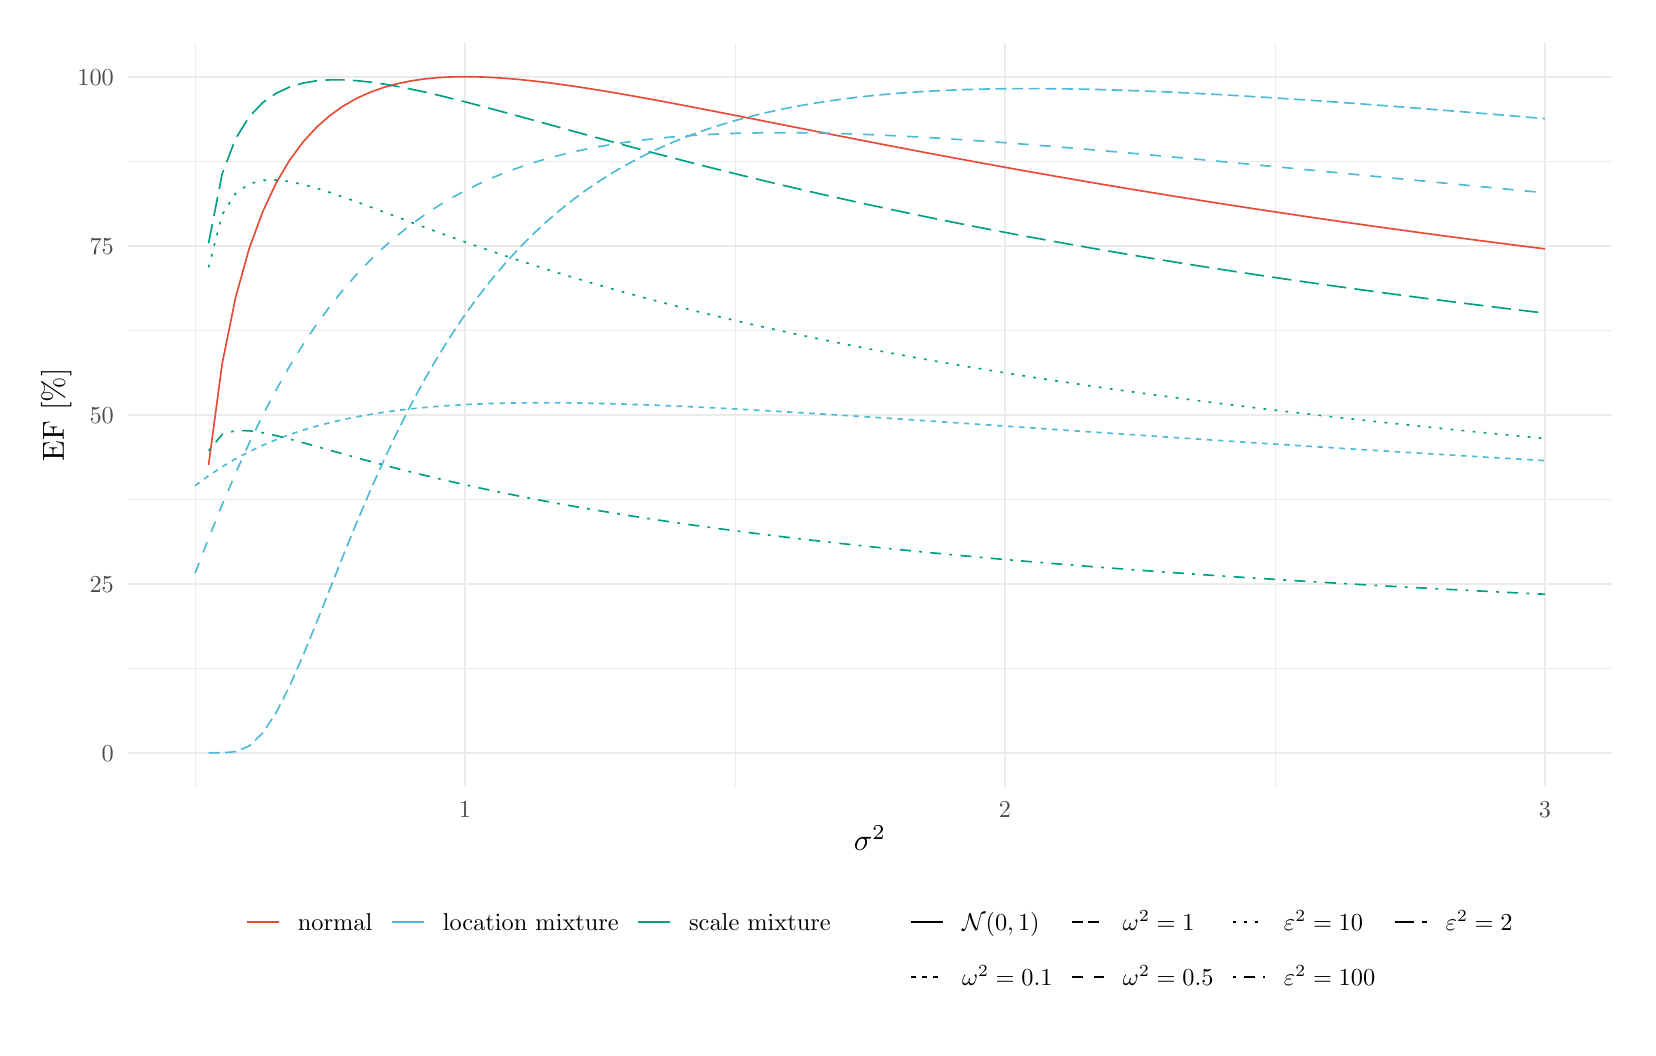
\begin{tikzpicture}[x=1pt,y=1pt]
\definecolor{fillColor}{RGB}{255,255,255}
\path[use as bounding box,fill=fillColor,fill opacity=0.00] (0,0) rectangle (578.16,361.35);
\begin{scope}
\path[clip] ( 36.11, 87.09) rectangle (572.66,355.85);
\definecolor{drawColor}{gray}{0.92}

\path[draw=drawColor,line width= 0.3pt,line join=round] ( 36.11,129.85) --
	(572.66,129.85);

\path[draw=drawColor,line width= 0.3pt,line join=round] ( 36.11,190.93) --
	(572.66,190.93);

\path[draw=drawColor,line width= 0.3pt,line join=round] ( 36.11,252.01) --
	(572.66,252.01);

\path[draw=drawColor,line width= 0.3pt,line join=round] ( 36.11,313.09) --
	(572.66,313.09);

\path[draw=drawColor,line width= 0.3pt,line join=round] ( 60.50, 87.09) --
	( 60.50,355.85);

\path[draw=drawColor,line width= 0.3pt,line join=round] (255.61, 87.09) --
	(255.61,355.85);

\path[draw=drawColor,line width= 0.3pt,line join=round] (450.72, 87.09) --
	(450.72,355.85);

\path[draw=drawColor,line width= 0.6pt,line join=round] ( 36.11, 99.31) --
	(572.66, 99.31);

\path[draw=drawColor,line width= 0.6pt,line join=round] ( 36.11,160.39) --
	(572.66,160.39);

\path[draw=drawColor,line width= 0.6pt,line join=round] ( 36.11,221.47) --
	(572.66,221.47);

\path[draw=drawColor,line width= 0.6pt,line join=round] ( 36.11,282.55) --
	(572.66,282.55);

\path[draw=drawColor,line width= 0.6pt,line join=round] ( 36.11,343.63) --
	(572.66,343.63);

\path[draw=drawColor,line width= 0.6pt,line join=round] (158.05, 87.09) --
	(158.05,355.85);

\path[draw=drawColor,line width= 0.6pt,line join=round] (353.16, 87.09) --
	(353.16,355.85);

\path[draw=drawColor,line width= 0.6pt,line join=round] (548.27, 87.09) --
	(548.27,355.85);
\definecolor{drawColor}{RGB}{230,75,53}

\path[draw=drawColor,line width= 0.6pt,line join=round] ( 65.38,203.37) --
	( 70.26,239.79) --
	( 75.13,263.88) --
	( 80.01,281.42) --
	( 84.89,294.77) --
	( 89.77,305.19) --
	( 94.64,313.45) --
	( 99.52,320.06) --
	(104.40,325.38) --
	(109.28,329.66) --
	(114.15,333.11) --
	(119.03,335.88) --
	(123.91,338.07) --
	(128.79,339.80) --
	(133.67,341.13) --
	(138.54,342.12) --
	(143.42,342.83) --
	(148.30,343.30) --
	(153.18,343.55) --
	(158.05,343.63) --
	(162.93,343.56) --
	(167.81,343.36) --
	(172.69,343.04) --
	(177.56,342.62) --
	(182.44,342.12) --
	(187.32,341.55) --
	(192.20,340.91) --
	(197.08,340.22) --
	(201.95,339.48) --
	(206.83,338.70) --
	(211.71,337.88) --
	(216.59,337.04) --
	(221.46,336.17) --
	(226.34,335.28) --
	(231.22,334.37) --
	(236.10,333.45) --
	(240.98,332.51) --
	(245.85,331.57) --
	(250.73,330.62) --
	(255.61,329.66) --
	(260.49,328.70) --
	(265.36,327.74) --
	(270.24,326.77) --
	(275.12,325.80) --
	(280.00,324.84) --
	(284.87,323.88) --
	(289.75,322.92) --
	(294.63,321.96) --
	(299.51,321.01) --
	(304.39,320.06) --
	(309.26,319.11) --
	(314.14,318.18) --
	(319.02,317.24) --
	(323.90,316.32) --
	(328.77,315.40) --
	(333.65,314.48) --
	(338.53,313.58) --
	(343.41,312.68) --
	(348.29,311.79) --
	(353.16,310.90) --
	(358.04,310.02) --
	(362.92,309.15) --
	(367.80,308.29) --
	(372.67,307.43) --
	(377.55,306.59) --
	(382.43,305.75) --
	(387.31,304.91) --
	(392.18,304.09) --
	(397.06,303.27) --
	(401.94,302.46) --
	(406.82,301.66) --
	(411.70,300.86) --
	(416.57,300.08) --
	(421.45,299.30) --
	(426.33,298.52) --
	(431.21,297.76) --
	(436.08,297.00) --
	(440.96,296.25) --
	(445.84,295.51) --
	(450.72,294.77) --
	(455.59,294.04) --
	(460.47,293.32) --
	(465.35,292.60) --
	(470.23,291.89) --
	(475.11,291.19) --
	(479.98,290.50) --
	(484.86,289.81) --
	(489.74,289.12) --
	(494.62,288.45) --
	(499.49,287.78) --
	(504.37,287.12) --
	(509.25,286.46) --
	(514.13,285.81) --
	(519.01,285.16) --
	(523.88,284.52) --
	(528.76,283.89) --
	(533.64,283.26) --
	(538.52,282.64) --
	(543.39,282.03) --
	(548.27,281.42);
\definecolor{drawColor}{RGB}{77,187,213}

\path[draw=drawColor,line width= 0.6pt,dash pattern=on 2pt off 2pt ,line join=round] ( 60.50,195.82) --
	( 65.38,199.43) --
	( 70.26,202.66) --
	( 75.13,205.55) --
	( 80.01,208.13) --
	( 84.89,210.43) --
	( 89.77,212.49) --
	( 94.64,214.31) --
	( 99.52,215.93) --
	(104.40,217.37) --
	(109.28,218.65) --
	(114.15,219.77) --
	(119.03,220.76) --
	(123.91,221.63) --
	(128.79,222.39) --
	(133.67,223.05) --
	(138.54,223.62) --
	(143.42,224.10) --
	(148.30,224.52) --
	(153.18,224.86) --
	(158.05,225.14) --
	(162.93,225.37) --
	(167.81,225.54) --
	(172.69,225.67) --
	(177.56,225.75) --
	(182.44,225.80) --
	(187.32,225.81) --
	(192.20,225.79) --
	(197.08,225.74) --
	(201.95,225.66) --
	(206.83,225.56) --
	(211.71,225.43) --
	(216.59,225.29) --
	(221.46,225.12) --
	(226.34,224.94) --
	(231.22,224.74) --
	(236.10,224.53) --
	(240.98,224.31) --
	(245.85,224.07) --
	(250.73,223.83) --
	(255.61,223.57) --
	(260.49,223.31) --
	(265.36,223.03) --
	(270.24,222.75) --
	(275.12,222.46) --
	(280.00,222.17) --
	(284.87,221.87) --
	(289.75,221.57) --
	(294.63,221.26) --
	(299.51,220.95) --
	(304.39,220.63) --
	(309.26,220.32) --
	(314.14,220.00) --
	(319.02,219.67) --
	(323.90,219.35) --
	(328.77,219.02) --
	(333.65,218.70) --
	(338.53,218.37) --
	(343.41,218.04) --
	(348.29,217.71) --
	(353.16,217.38) --
	(358.04,217.05) --
	(362.92,216.71) --
	(367.80,216.38) --
	(372.67,216.05) --
	(377.55,215.72) --
	(382.43,215.39) --
	(387.31,215.06) --
	(392.18,214.73) --
	(397.06,214.41) --
	(401.94,214.08) --
	(406.82,213.75) --
	(411.70,213.43) --
	(416.57,213.10) --
	(421.45,212.78) --
	(426.33,212.46) --
	(431.21,212.14) --
	(436.08,211.82) --
	(440.96,211.50) --
	(445.84,211.18) --
	(450.72,210.87) --
	(455.59,210.56) --
	(460.47,210.24) --
	(465.35,209.93) --
	(470.23,209.63) --
	(475.11,209.32) --
	(479.98,209.01) --
	(484.86,208.71) --
	(489.74,208.41) --
	(494.62,208.11) --
	(499.49,207.81) --
	(504.37,207.51) --
	(509.25,207.21) --
	(514.13,206.92) --
	(519.01,206.63) --
	(523.88,206.34) --
	(528.76,206.05) --
	(533.64,205.76) --
	(538.52,205.48) --
	(543.39,205.19) --
	(548.27,204.91);

\path[draw=drawColor,line width= 0.6pt,dash pattern=on 4pt off 2pt ,line join=round] ( 65.38, 99.31) --
	( 70.26, 99.32) --
	( 75.13, 99.73) --
	( 80.01,101.76) --
	( 84.89,106.42) --
	( 89.77,113.81) --
	( 94.64,123.40) --
	( 99.52,134.49) --
	(104.40,146.43) --
	(109.28,158.70) --
	(114.15,170.93) --
	(119.03,182.87) --
	(123.91,194.33) --
	(128.79,205.24) --
	(133.67,215.53) --
	(138.54,225.18) --
	(143.42,234.19) --
	(148.30,242.59) --
	(153.18,250.40) --
	(158.05,257.65) --
	(162.93,264.36) --
	(167.81,270.57) --
	(172.69,276.33) --
	(177.56,281.64) --
	(182.44,286.56) --
	(187.32,291.11) --
	(192.20,295.30) --
	(197.08,299.18) --
	(201.95,302.76) --
	(206.83,306.07) --
	(211.71,309.12) --
	(216.59,311.94) --
	(221.46,314.53) --
	(226.34,316.93) --
	(231.22,319.13) --
	(236.10,321.16) --
	(240.98,323.03) --
	(245.85,324.74) --
	(250.73,326.32) --
	(255.61,327.76) --
	(260.49,329.09) --
	(265.36,330.30) --
	(270.24,331.40) --
	(275.12,332.41) --
	(280.00,333.32) --
	(284.87,334.15) --
	(289.75,334.90) --
	(294.63,335.57) --
	(299.51,336.17) --
	(304.39,336.71) --
	(309.26,337.19) --
	(314.14,337.61) --
	(319.02,337.97) --
	(323.90,338.29) --
	(328.77,338.55) --
	(333.65,338.78) --
	(338.53,338.96) --
	(343.41,339.10) --
	(348.29,339.21) --
	(353.16,339.28) --
	(358.04,339.32) --
	(362.92,339.33) --
	(367.80,339.31) --
	(372.67,339.26) --
	(377.55,339.19) --
	(382.43,339.10) --
	(387.31,338.98) --
	(392.18,338.84) --
	(397.06,338.68) --
	(401.94,338.51) --
	(406.82,338.32) --
	(411.70,338.11) --
	(416.57,337.88) --
	(421.45,337.64) --
	(426.33,337.39) --
	(431.21,337.13) --
	(436.08,336.85) --
	(440.96,336.56) --
	(445.84,336.26) --
	(450.72,335.96) --
	(455.59,335.64) --
	(460.47,335.31) --
	(465.35,334.98) --
	(470.23,334.64) --
	(475.11,334.29) --
	(479.98,333.94) --
	(484.86,333.57) --
	(489.74,333.21) --
	(494.62,332.84) --
	(499.49,332.46) --
	(504.37,332.08) --
	(509.25,331.69) --
	(514.13,331.30) --
	(519.01,330.91) --
	(523.88,330.51) --
	(528.76,330.11) --
	(533.64,329.71) --
	(538.52,329.30) --
	(543.39,328.89) --
	(548.27,328.48);

\path[draw=drawColor,line width= 0.6pt,dash pattern=on 4pt off 4pt ,line join=round] ( 60.50,164.25) --
	( 65.38,176.83) --
	( 70.26,188.93) --
	( 75.13,200.39) --
	( 80.01,211.15) --
	( 84.89,221.17) --
	( 89.77,230.45) --
	( 94.64,239.01) --
	( 99.52,246.89) --
	(104.40,254.12) --
	(109.28,260.75) --
	(114.15,266.83) --
	(119.03,272.38) --
	(123.91,277.45) --
	(128.79,282.09) --
	(133.67,286.32) --
	(138.54,290.17) --
	(143.42,293.69) --
	(148.30,296.89) --
	(153.18,299.81) --
	(158.05,302.46) --
	(162.93,304.87) --
	(167.81,307.06) --
	(172.69,309.05) --
	(177.56,310.84) --
	(182.44,312.46) --
	(187.32,313.93) --
	(192.20,315.25) --
	(197.08,316.43) --
	(201.95,317.49) --
	(206.83,318.43) --
	(211.71,319.26) --
	(216.59,320.00) --
	(221.46,320.65) --
	(226.34,321.21) --
	(231.22,321.70) --
	(236.10,322.11) --
	(240.98,322.46) --
	(245.85,322.74) --
	(250.73,322.97) --
	(255.61,323.15) --
	(260.49,323.27) --
	(265.36,323.35) --
	(270.24,323.39) --
	(275.12,323.39) --
	(280.00,323.35) --
	(284.87,323.27) --
	(289.75,323.17) --
	(294.63,323.04) --
	(299.51,322.88) --
	(304.39,322.69) --
	(309.26,322.48) --
	(314.14,322.25) --
	(319.02,322.00) --
	(323.90,321.72) --
	(328.77,321.44) --
	(333.65,321.13) --
	(338.53,320.81) --
	(343.41,320.48) --
	(348.29,320.13) --
	(353.16,319.77) --
	(358.04,319.40) --
	(362.92,319.02) --
	(367.80,318.63) --
	(372.67,318.24) --
	(377.55,317.83) --
	(382.43,317.42) --
	(387.31,317.00) --
	(392.18,316.57) --
	(397.06,316.14) --
	(401.94,315.70) --
	(406.82,315.26) --
	(411.70,314.81) --
	(416.57,314.36) --
	(421.45,313.90) --
	(426.33,313.45) --
	(431.21,312.99) --
	(436.08,312.52) --
	(440.96,312.06) --
	(445.84,311.59) --
	(450.72,311.12) --
	(455.59,310.65) --
	(460.47,310.18) --
	(465.35,309.71) --
	(470.23,309.24) --
	(475.11,308.76) --
	(479.98,308.29) --
	(484.86,307.81) --
	(489.74,307.34) --
	(494.62,306.86) --
	(499.49,306.39) --
	(504.37,305.92) --
	(509.25,305.44) --
	(514.13,304.97) --
	(519.01,304.50) --
	(523.88,304.02) --
	(528.76,303.55) --
	(533.64,303.08) --
	(538.52,302.61) --
	(543.39,302.15) --
	(548.27,301.68);
\definecolor{drawColor}{RGB}{0,160,135}

\path[draw=drawColor,line width= 0.6pt,dash pattern=on 1pt off 3pt ,line join=round] ( 65.38,274.74) --
	( 70.26,293.74) --
	( 75.13,301.44) --
	( 80.01,304.87) --
	( 84.89,306.20) --
	( 89.77,306.33) --
	( 94.64,305.74) --
	( 99.52,304.68) --
	(104.40,303.33) --
	(109.28,301.78) --
	(114.15,300.11) --
	(119.03,298.35) --
	(123.91,296.55) --
	(128.79,294.72) --
	(133.67,292.88) --
	(138.54,291.05) --
	(143.42,289.23) --
	(148.30,287.43) --
	(153.18,285.66) --
	(158.05,283.91) --
	(162.93,282.19) --
	(167.81,280.51) --
	(172.69,278.86) --
	(177.56,277.24) --
	(182.44,275.65) --
	(187.32,274.10) --
	(192.20,272.58) --
	(197.08,271.09) --
	(201.95,269.63) --
	(206.83,268.21) --
	(211.71,266.82) --
	(216.59,265.45) --
	(221.46,264.12) --
	(226.34,262.81) --
	(231.22,261.54) --
	(236.10,260.28) --
	(240.98,259.06) --
	(245.85,257.86) --
	(250.73,256.68) --
	(255.61,255.53) --
	(260.49,254.41) --
	(265.36,253.30) --
	(270.24,252.22) --
	(275.12,251.16) --
	(280.00,250.12) --
	(284.87,249.09) --
	(289.75,248.09) --
	(294.63,247.11) --
	(299.51,246.15) --
	(304.39,245.20) --
	(309.26,244.27) --
	(314.14,243.36) --
	(319.02,242.46) --
	(323.90,241.58) --
	(328.77,240.72) --
	(333.65,239.87) --
	(338.53,239.04) --
	(343.41,238.22) --
	(348.29,237.41) --
	(353.16,236.62) --
	(358.04,235.84) --
	(362.92,235.07) --
	(367.80,234.32) --
	(372.67,233.58) --
	(377.55,232.85) --
	(382.43,232.13) --
	(387.31,231.42) --
	(392.18,230.72) --
	(397.06,230.04) --
	(401.94,229.36) --
	(406.82,228.70) --
	(411.70,228.04) --
	(416.57,227.40) --
	(421.45,226.76) --
	(426.33,226.13) --
	(431.21,225.51) --
	(436.08,224.91) --
	(440.96,224.31) --
	(445.84,223.71) --
	(450.72,223.13) --
	(455.59,222.55) --
	(460.47,221.99) --
	(465.35,221.43) --
	(470.23,220.87) --
	(475.11,220.33) --
	(479.98,219.79) --
	(484.86,219.26) --
	(489.74,218.73) --
	(494.62,218.22) --
	(499.49,217.71) --
	(504.37,217.20) --
	(509.25,216.70) --
	(514.13,216.21) --
	(519.01,215.72) --
	(523.88,215.24) --
	(528.76,214.77) --
	(533.64,214.30) --
	(538.52,213.84) --
	(543.39,213.38) --
	(548.27,212.93);

\path[draw=drawColor,line width= 0.6pt,dash pattern=on 1pt off 3pt on 4pt off 3pt ,line join=round] ( 65.38,208.48) --
	( 70.26,214.33) --
	( 75.13,215.76) --
	( 80.01,215.71) --
	( 84.89,214.99) --
	( 89.77,213.93) --
	( 94.64,212.70) --
	( 99.52,211.37) --
	(104.40,210.01) --
	(109.28,208.63) --
	(114.15,207.26) --
	(119.03,205.90) --
	(123.91,204.58) --
	(128.79,203.28) --
	(133.67,202.01) --
	(138.54,200.78) --
	(143.42,199.58) --
	(148.30,198.41) --
	(153.18,197.28) --
	(158.05,196.18) --
	(162.93,195.11) --
	(167.81,194.07) --
	(172.69,193.07) --
	(177.56,192.09) --
	(182.44,191.13) --
	(187.32,190.21) --
	(192.20,189.31) --
	(197.08,188.44) --
	(201.95,187.58) --
	(206.83,186.76) --
	(211.71,185.95) --
	(216.59,185.16) --
	(221.46,184.40) --
	(226.34,183.65) --
	(231.22,182.92) --
	(236.10,182.21) --
	(240.98,181.52) --
	(245.85,180.85) --
	(250.73,180.19) --
	(255.61,179.54) --
	(260.49,178.91) --
	(265.36,178.30) --
	(270.24,177.70) --
	(275.12,177.11) --
	(280.00,176.53) --
	(284.87,175.97) --
	(289.75,175.42) --
	(294.63,174.88) --
	(299.51,174.35) --
	(304.39,173.83) --
	(309.26,173.32) --
	(314.14,172.83) --
	(319.02,172.34) --
	(323.90,171.86) --
	(328.77,171.39) --
	(333.65,170.93) --
	(338.53,170.48) --
	(343.41,170.04) --
	(348.29,169.60) --
	(353.16,169.17) --
	(358.04,168.75) --
	(362.92,168.34) --
	(367.80,167.94) --
	(372.67,167.54) --
	(377.55,167.15) --
	(382.43,166.76) --
	(387.31,166.38) --
	(392.18,166.01) --
	(397.06,165.65) --
	(401.94,165.29) --
	(406.82,164.93) --
	(411.70,164.58) --
	(416.57,164.24) --
	(421.45,163.90) --
	(426.33,163.57) --
	(431.21,163.24) --
	(436.08,162.92) --
	(440.96,162.60) --
	(445.84,162.29) --
	(450.72,161.98) --
	(455.59,161.68) --
	(460.47,161.38) --
	(465.35,161.08) --
	(470.23,160.79) --
	(475.11,160.50) --
	(479.98,160.22) --
	(484.86,159.94) --
	(489.74,159.66) --
	(494.62,159.39) --
	(499.49,159.12) --
	(504.37,158.86) --
	(509.25,158.60) --
	(514.13,158.34) --
	(519.01,158.08) --
	(523.88,157.83) --
	(528.76,157.58) --
	(533.64,157.34) --
	(538.52,157.10) --
	(543.39,156.86) --
	(548.27,156.62);

\path[draw=drawColor,line width= 0.6pt,dash pattern=on 7pt off 3pt ,line join=round] ( 65.38,283.45) --
	( 70.26,308.45) --
	( 75.13,321.26) --
	( 80.01,329.09) --
	( 84.89,334.21) --
	( 89.77,337.63) --
	( 94.64,339.90) --
	( 99.52,341.33) --
	(104.40,342.15) --
	(109.28,342.50) --
	(114.15,342.48) --
	(119.03,342.18) --
	(123.91,341.66) --
	(128.79,340.95) --
	(133.67,340.11) --
	(138.54,339.14) --
	(143.42,338.09) --
	(148.30,336.96) --
	(153.18,335.77) --
	(158.05,334.54) --
	(162.93,333.27) --
	(167.81,331.97) --
	(172.69,330.66) --
	(177.56,329.33) --
	(182.44,327.99) --
	(187.32,326.65) --
	(192.20,325.30) --
	(197.08,323.96) --
	(201.95,322.62) --
	(206.83,321.29) --
	(211.71,319.97) --
	(216.59,318.65) --
	(221.46,317.35) --
	(226.34,316.05) --
	(231.22,314.77) --
	(236.10,313.51) --
	(240.98,312.25) --
	(245.85,311.01) --
	(250.73,309.79) --
	(255.61,308.58) --
	(260.49,307.38) --
	(265.36,306.20) --
	(270.24,305.03) --
	(275.12,303.88) --
	(280.00,302.74) --
	(284.87,301.62) --
	(289.75,300.51) --
	(294.63,299.42) --
	(299.51,298.34) --
	(304.39,297.28) --
	(309.26,296.23) --
	(314.14,295.19) --
	(319.02,294.17) --
	(323.90,293.16) --
	(328.77,292.16) --
	(333.65,291.18) --
	(338.53,290.21) --
	(343.41,289.26) --
	(348.29,288.31) --
	(353.16,287.38) --
	(358.04,286.46) --
	(362.92,285.56) --
	(367.80,284.66) --
	(372.67,283.78) --
	(377.55,282.91) --
	(382.43,282.04) --
	(387.31,281.19) --
	(392.18,280.36) --
	(397.06,279.53) --
	(401.94,278.71) --
	(406.82,277.90) --
	(411.70,277.10) --
	(416.57,276.31) --
	(421.45,275.54) --
	(426.33,274.77) --
	(431.21,274.01) --
	(436.08,273.26) --
	(440.96,272.52) --
	(445.84,271.79) --
	(450.72,271.06) --
	(455.59,270.35) --
	(460.47,269.64) --
	(465.35,268.94) --
	(470.23,268.25) --
	(475.11,267.57) --
	(479.98,266.89) --
	(484.86,266.23) --
	(489.74,265.57) --
	(494.62,264.92) --
	(499.49,264.27) --
	(504.37,263.63) --
	(509.25,263.00) --
	(514.13,262.38) --
	(519.01,261.76) --
	(523.88,261.15) --
	(528.76,260.55) --
	(533.64,259.95) --
	(538.52,259.36) --
	(543.39,258.78) --
	(548.27,258.20);
\end{scope}
\begin{scope}
\path[clip] (  0.00,  0.00) rectangle (578.16,361.35);
\definecolor{drawColor}{gray}{0.30}

\node[text=drawColor,anchor=base east,inner sep=0pt, outer sep=0pt, scale=  0.88] at ( 31.16, 96.28) {0};

\node[text=drawColor,anchor=base east,inner sep=0pt, outer sep=0pt, scale=  0.88] at ( 31.16,157.36) {25};

\node[text=drawColor,anchor=base east,inner sep=0pt, outer sep=0pt, scale=  0.88] at ( 31.16,218.44) {50};

\node[text=drawColor,anchor=base east,inner sep=0pt, outer sep=0pt, scale=  0.88] at ( 31.16,279.52) {75};

\node[text=drawColor,anchor=base east,inner sep=0pt, outer sep=0pt, scale=  0.88] at ( 31.16,340.60) {100};
\end{scope}
\begin{scope}
\path[clip] (  0.00,  0.00) rectangle (578.16,361.35);
\definecolor{drawColor}{gray}{0.30}

\node[text=drawColor,anchor=base,inner sep=0pt, outer sep=0pt, scale=  0.88] at (158.05, 76.08) {1};

\node[text=drawColor,anchor=base,inner sep=0pt, outer sep=0pt, scale=  0.88] at (353.16, 76.08) {2};

\node[text=drawColor,anchor=base,inner sep=0pt, outer sep=0pt, scale=  0.88] at (548.27, 76.08) {3};
\end{scope}
\begin{scope}
\path[clip] (  0.00,  0.00) rectangle (578.16,361.35);
\definecolor{drawColor}{RGB}{0,0,0}

\node[text=drawColor,anchor=base,inner sep=0pt, outer sep=0pt, scale=  1.10] at (304.39, 64.05) {$\sigma^2$};
\end{scope}
\begin{scope}
\path[clip] (  0.00,  0.00) rectangle (578.16,361.35);
\definecolor{drawColor}{RGB}{0,0,0}

\node[text=drawColor,rotate= 90.00,anchor=base,inner sep=0pt, outer sep=0pt, scale=  1.10] at ( 13.08,221.47) {EF [\%]};
\end{scope}
\begin{scope}
\path[clip] (  0.00,  0.00) rectangle (578.16,361.35);
\definecolor{drawColor}{RGB}{230,75,53}

\path[draw=drawColor,line width= 0.6pt,line join=round] ( 79.13, 38.18) -- ( 90.69, 38.18);
\end{scope}
\begin{scope}
\path[clip] (  0.00,  0.00) rectangle (578.16,361.35);
\definecolor{drawColor}{RGB}{77,187,213}

\path[draw=drawColor,line width= 0.6pt,line join=round] (131.49, 38.18) -- (143.05, 38.18);
\end{scope}
\begin{scope}
\path[clip] (  0.00,  0.00) rectangle (578.16,361.35);
\definecolor{drawColor}{RGB}{0,160,135}

\path[draw=drawColor,line width= 0.6pt,line join=round] (220.51, 38.18) -- (232.07, 38.18);
\end{scope}
\begin{scope}
\path[clip] (  0.00,  0.00) rectangle (578.16,361.35);
\definecolor{drawColor}{RGB}{0,0,0}

\node[text=drawColor,anchor=base west,inner sep=0pt, outer sep=0pt, scale=  0.88] at ( 97.64, 35.15) {normal};
\end{scope}
\begin{scope}
\path[clip] (  0.00,  0.00) rectangle (578.16,361.35);
\definecolor{drawColor}{RGB}{0,0,0}

\node[text=drawColor,anchor=base west,inner sep=0pt, outer sep=0pt, scale=  0.88] at (150.00, 35.15) {location mixture};
\end{scope}
\begin{scope}
\path[clip] (  0.00,  0.00) rectangle (578.16,361.35);
\definecolor{drawColor}{RGB}{0,0,0}

\node[text=drawColor,anchor=base west,inner sep=0pt, outer sep=0pt, scale=  0.88] at (239.02, 35.15) {scale mixture};
\end{scope}
\begin{scope}
\path[clip] (  0.00,  0.00) rectangle (578.16,361.35);
\definecolor{drawColor}{RGB}{0,0,0}

\path[draw=drawColor,line width= 0.6pt,line join=round] (319.11, 38.18) -- (330.67, 38.18);
\end{scope}
\begin{scope}
\path[clip] (  0.00,  0.00) rectangle (578.16,361.35);
\definecolor{drawColor}{RGB}{0,0,0}

\path[draw=drawColor,line width= 0.6pt,dash pattern=on 2pt off 2pt ,line join=round] (319.11, 18.23) -- (330.67, 18.23);
\end{scope}
\begin{scope}
\path[clip] (  0.00,  0.00) rectangle (578.16,361.35);
\definecolor{drawColor}{RGB}{0,0,0}

\path[draw=drawColor,line width= 0.6pt,dash pattern=on 4pt off 2pt ,line join=round] (377.28, 38.18) -- (388.85, 38.18);
\end{scope}
\begin{scope}
\path[clip] (  0.00,  0.00) rectangle (578.16,361.35);
\definecolor{drawColor}{RGB}{0,0,0}

\path[draw=drawColor,line width= 0.6pt,dash pattern=on 4pt off 4pt ,line join=round] (377.28, 18.23) -- (388.85, 18.23);
\end{scope}
\begin{scope}
\path[clip] (  0.00,  0.00) rectangle (578.16,361.35);
\definecolor{drawColor}{RGB}{0,0,0}

\path[draw=drawColor,line width= 0.6pt,dash pattern=on 1pt off 3pt ,line join=round] (435.46, 38.18) -- (447.02, 38.18);
\end{scope}
\begin{scope}
\path[clip] (  0.00,  0.00) rectangle (578.16,361.35);
\definecolor{drawColor}{RGB}{0,0,0}

\path[draw=drawColor,line width= 0.6pt,dash pattern=on 1pt off 3pt on 4pt off 3pt ,line join=round] (435.46, 18.23) -- (447.02, 18.23);
\end{scope}
\begin{scope}
\path[clip] (  0.00,  0.00) rectangle (578.16,361.35);
\definecolor{drawColor}{RGB}{0,0,0}

\path[draw=drawColor,line width= 0.6pt,dash pattern=on 7pt off 3pt ,line join=round] (493.90, 38.18) -- (505.46, 38.18);
\end{scope}
\begin{scope}
\path[clip] (  0.00,  0.00) rectangle (578.16,361.35);
\definecolor{drawColor}{RGB}{0,0,0}

\node[text=drawColor,anchor=base west,inner sep=0pt, outer sep=0pt, scale=  0.88] at (337.62, 35.15) {$\mathcal N (0, 1)$};
\end{scope}
\begin{scope}
\path[clip] (  0.00,  0.00) rectangle (578.16,361.35);
\definecolor{drawColor}{RGB}{0,0,0}

\node[text=drawColor,anchor=base west,inner sep=0pt, outer sep=0pt, scale=  0.88] at (337.62, 15.20) {$\omega^2 = 0.1$};
\end{scope}
\begin{scope}
\path[clip] (  0.00,  0.00) rectangle (578.16,361.35);
\definecolor{drawColor}{RGB}{0,0,0}

\node[text=drawColor,anchor=base west,inner sep=0pt, outer sep=0pt, scale=  0.88] at (395.79, 35.15) {$\omega^2 = 1$};
\end{scope}
\begin{scope}
\path[clip] (  0.00,  0.00) rectangle (578.16,361.35);
\definecolor{drawColor}{RGB}{0,0,0}

\node[text=drawColor,anchor=base west,inner sep=0pt, outer sep=0pt, scale=  0.88] at (395.79, 15.20) {$\omega^2= 0.5$};
\end{scope}
\begin{scope}
\path[clip] (  0.00,  0.00) rectangle (578.16,361.35);
\definecolor{drawColor}{RGB}{0,0,0}

\node[text=drawColor,anchor=base west,inner sep=0pt, outer sep=0pt, scale=  0.88] at (453.97, 35.15) {$\varepsilon^2 = 10$};
\end{scope}
\begin{scope}
\path[clip] (  0.00,  0.00) rectangle (578.16,361.35);
\definecolor{drawColor}{RGB}{0,0,0}

\node[text=drawColor,anchor=base west,inner sep=0pt, outer sep=0pt, scale=  0.88] at (453.97, 15.20) {$\varepsilon^2 = 100$};
\end{scope}
\begin{scope}
\path[clip] (  0.00,  0.00) rectangle (578.16,361.35);
\definecolor{drawColor}{RGB}{0,0,0}

\node[text=drawColor,anchor=base west,inner sep=0pt, outer sep=0pt, scale=  0.88] at (512.40, 35.15) {$\varepsilon^2 = 2$};
\end{scope}
\end{tikzpicture}
%
    }
    \caption{{\color{red}} TODO}
    \label{fig:rho_mu}

\end{figure}
% fig:rho_mu
%% except for location mixture w/ large omega^2 all EF quite high, 
%% allows for misspecification in variance here, except to small for location mixture w/ large omega2
%% better too have large sigma2 than small -> EIS better than CE? 

For \Cref{ex:univ-gaussian-mu-fixed} the two methods have different optimal proposals, thus also different asymptotic efficiency factors. In \Cref{fig:rho}, the first two subfigures show how the efficiency factor depends on the misspecified $mu$ for both methods. The optimal variances are based on the results from \Cref{ex:univ-gaussian-mu-fixed}, i.e. based on simulation for \aeis. The right-hand subfigure shows the relative efficiency factor, i.e. the ratio of the efficiency factor for the \acem and \aeis. Here values smaller than $1$ indicate that \aeis has a larger efficiency factor than the \acem. 

\begin{figure}
    \centering

    \resizebox{\textwidth}{!}{%
        % Created by tikzDevice version 0.12.6 on 2024-06-10 10:41:39
% !TEX encoding = UTF-8 Unicode
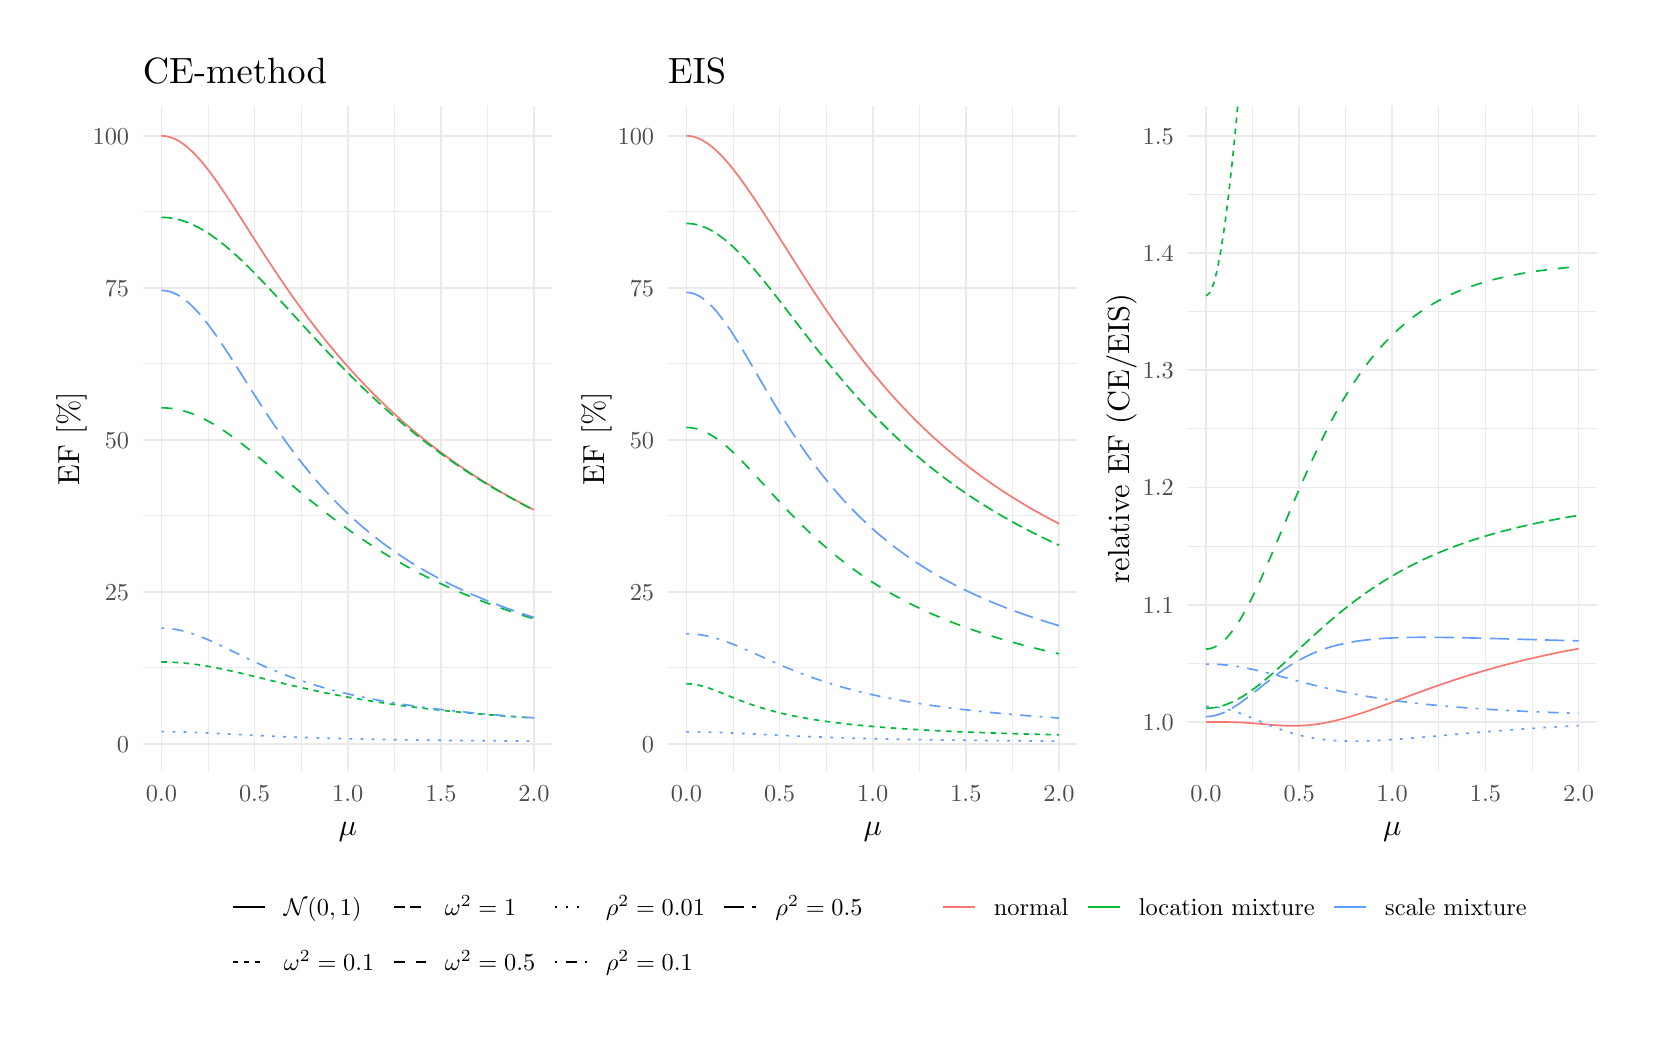
\begin{tikzpicture}[x=1pt,y=1pt]
\definecolor{fillColor}{RGB}{255,255,255}
\path[use as bounding box,fill=fillColor,fill opacity=0.00] (0,0) rectangle (578.16,361.35);
\begin{scope}
\path[clip] ( 41.61, 92.59) rectangle (189.71,333.19);
\definecolor{drawColor}{gray}{0.92}

\path[draw=drawColor,line width= 0.3pt,line join=round] ( 41.61,130.05) --
	(189.71,130.05);

\path[draw=drawColor,line width= 0.3pt,line join=round] ( 41.61,184.97) --
	(189.71,184.97);

\path[draw=drawColor,line width= 0.3pt,line join=round] ( 41.61,239.88) --
	(189.71,239.88);

\path[draw=drawColor,line width= 0.3pt,line join=round] ( 41.61,294.80) --
	(189.71,294.80);

\path[draw=drawColor,line width= 0.3pt,line join=round] ( 65.17, 92.59) --
	( 65.17,333.19);

\path[draw=drawColor,line width= 0.3pt,line join=round] ( 98.83, 92.59) --
	( 98.83,333.19);

\path[draw=drawColor,line width= 0.3pt,line join=round] (132.49, 92.59) --
	(132.49,333.19);

\path[draw=drawColor,line width= 0.3pt,line join=round] (166.14, 92.59) --
	(166.14,333.19);

\path[draw=drawColor,line width= 0.6pt,line join=round] ( 41.61,102.59) --
	(189.71,102.59);

\path[draw=drawColor,line width= 0.6pt,line join=round] ( 41.61,157.51) --
	(189.71,157.51);

\path[draw=drawColor,line width= 0.6pt,line join=round] ( 41.61,212.42) --
	(189.71,212.42);

\path[draw=drawColor,line width= 0.6pt,line join=round] ( 41.61,267.34) --
	(189.71,267.34);

\path[draw=drawColor,line width= 0.6pt,line join=round] ( 41.61,322.26) --
	(189.71,322.26);

\path[draw=drawColor,line width= 0.6pt,line join=round] ( 48.34, 92.59) --
	( 48.34,333.19);

\path[draw=drawColor,line width= 0.6pt,line join=round] ( 82.00, 92.59) --
	( 82.00,333.19);

\path[draw=drawColor,line width= 0.6pt,line join=round] (115.66, 92.59) --
	(115.66,333.19);

\path[draw=drawColor,line width= 0.6pt,line join=round] (149.32, 92.59) --
	(149.32,333.19);

\path[draw=drawColor,line width= 0.6pt,line join=round] (182.97, 92.59) --
	(182.97,333.19);
\definecolor{drawColor}{RGB}{248,118,109}

\path[draw=drawColor,line width= 0.6pt,line join=round] ( 48.34,322.26) --
	( 49.69,322.17) --
	( 51.04,321.91) --
	( 52.38,321.47) --
	( 53.73,320.87) --
	( 55.07,320.10) --
	( 56.42,319.18) --
	( 57.77,318.11) --
	( 59.11,316.90) --
	( 60.46,315.57) --
	( 61.81,314.11) --
	( 63.15,312.55) --
	( 64.50,310.89) --
	( 65.84,309.14) --
	( 67.19,307.32) --
	( 68.54,305.43) --
	( 69.88,303.49) --
	( 71.23,301.49) --
	( 72.58,299.46) --
	( 73.92,297.40) --
	( 75.27,295.32) --
	( 76.62,293.22) --
	( 77.96,291.11) --
	( 79.31,289.00) --
	( 80.65,286.89) --
	( 82.00,284.78) --
	( 83.35,282.68) --
	( 84.69,280.59) --
	( 86.04,278.51) --
	( 87.39,276.46) --
	( 88.73,274.42) --
	( 90.08,272.40) --
	( 91.42,270.40) --
	( 92.77,268.43) --
	( 94.12,266.48) --
	( 95.46,264.56) --
	( 96.81,262.66) --
	( 98.16,260.79) --
	( 99.50,258.95) --
	(100.85,257.13) --
	(102.20,255.34) --
	(103.54,253.58) --
	(104.89,251.84) --
	(106.23,250.13) --
	(107.58,248.45) --
	(108.93,246.79) --
	(110.27,245.16) --
	(111.62,243.56) --
	(112.97,241.98) --
	(114.31,240.43) --
	(115.66,238.90) --
	(117.00,237.40) --
	(118.35,235.92) --
	(119.70,234.47) --
	(121.04,233.04) --
	(122.39,231.63) --
	(123.74,230.25) --
	(125.08,228.89) --
	(126.43,227.55) --
	(127.77,226.24) --
	(129.12,224.94) --
	(130.47,223.67) --
	(131.81,222.42) --
	(133.16,221.19) --
	(134.51,219.97) --
	(135.85,218.78) --
	(137.20,217.61) --
	(138.55,216.46) --
	(139.89,215.32) --
	(141.24,214.21) --
	(142.58,213.11) --
	(143.93,212.03) --
	(145.28,210.97) --
	(146.62,209.92) --
	(147.97,208.89) --
	(149.32,207.88) --
	(150.66,206.89) --
	(152.01,205.91) --
	(153.35,204.94) --
	(154.70,203.99) --
	(156.05,203.06) --
	(157.39,202.14) --
	(158.74,201.23) --
	(160.09,200.34) --
	(161.43,199.46) --
	(162.78,198.60) --
	(164.13,197.75) --
	(165.47,196.91) --
	(166.82,196.09) --
	(168.16,195.27) --
	(169.51,194.47) --
	(170.86,193.68) --
	(172.20,192.91) --
	(173.55,192.14) --
	(174.90,191.39) --
	(176.24,190.65) --
	(177.59,189.92) --
	(178.93,189.20) --
	(180.28,188.49) --
	(181.63,187.79) --
	(182.97,187.10);
\definecolor{drawColor}{RGB}{0,186,56}

\path[draw=drawColor,line width= 0.6pt,dash pattern=on 2pt off 2pt ,line join=round] ( 48.34,132.14) --
	( 49.69,132.13) --
	( 51.04,132.09) --
	( 52.38,132.04) --
	( 53.73,131.97) --
	( 55.07,131.87) --
	( 56.42,131.76) --
	( 57.77,131.62) --
	( 59.11,131.47) --
	( 60.46,131.30) --
	( 61.81,131.11) --
	( 63.15,130.90) --
	( 64.50,130.68) --
	( 65.84,130.45) --
	( 67.19,130.20) --
	( 68.54,129.94) --
	( 69.88,129.67) --
	( 71.23,129.39) --
	( 72.58,129.10) --
	( 73.92,128.80) --
	( 75.27,128.50) --
	( 76.62,128.19) --
	( 77.96,127.87) --
	( 79.31,127.55) --
	( 80.65,127.23) --
	( 82.00,126.91) --
	( 83.35,126.58) --
	( 84.69,126.25) --
	( 86.04,125.92) --
	( 87.39,125.59) --
	( 88.73,125.27) --
	( 90.08,124.94) --
	( 91.42,124.62) --
	( 92.77,124.30) --
	( 94.12,123.98) --
	( 95.46,123.66) --
	( 96.81,123.35) --
	( 98.16,123.04) --
	( 99.50,122.74) --
	(100.85,122.44) --
	(102.20,122.14) --
	(103.54,121.85) --
	(104.89,121.57) --
	(106.23,121.29) --
	(107.58,121.01) --
	(108.93,120.74) --
	(110.27,120.47) --
	(111.62,120.21) --
	(112.97,119.95) --
	(114.31,119.70) --
	(115.66,119.46) --
	(117.00,119.21) --
	(118.35,118.98) --
	(119.70,118.74) --
	(121.04,118.52) --
	(122.39,118.29) --
	(123.74,118.08) --
	(125.08,117.86) --
	(126.43,117.65) --
	(127.77,117.45) --
	(129.12,117.25) --
	(130.47,117.05) --
	(131.81,116.86) --
	(133.16,116.67) --
	(134.51,116.49) --
	(135.85,116.31) --
	(137.20,116.13) --
	(138.55,115.96) --
	(139.89,115.79) --
	(141.24,115.63) --
	(142.58,115.47) --
	(143.93,115.31) --
	(145.28,115.15) --
	(146.62,115.00) --
	(147.97,114.85) --
	(149.32,114.71) --
	(150.66,114.56) --
	(152.01,114.42) --
	(153.35,114.29) --
	(154.70,114.15) --
	(156.05,114.02) --
	(157.39,113.89) --
	(158.74,113.77) --
	(160.09,113.65) --
	(161.43,113.52) --
	(162.78,113.41) --
	(164.13,113.29) --
	(165.47,113.18) --
	(166.82,113.06) --
	(168.16,112.95) --
	(169.51,112.85) --
	(170.86,112.74) --
	(172.20,112.64) --
	(173.55,112.54) --
	(174.90,112.44) --
	(176.24,112.34) --
	(177.59,112.24) --
	(178.93,112.15) --
	(180.28,112.06) --
	(181.63,111.97) --
	(182.97,111.88);

\path[draw=drawColor,line width= 0.6pt,dash pattern=on 4pt off 2pt ,line join=round] ( 48.34,292.80) --
	( 49.69,292.76) --
	( 51.04,292.65) --
	( 52.38,292.46) --
	( 53.73,292.20) --
	( 55.07,291.86) --
	( 56.42,291.45) --
	( 57.77,290.96) --
	( 59.11,290.41) --
	( 60.46,289.79) --
	( 61.81,289.10) --
	( 63.15,288.35) --
	( 64.50,287.54) --
	( 65.84,286.67) --
	( 67.19,285.74) --
	( 68.54,284.76) --
	( 69.88,283.73) --
	( 71.23,282.65) --
	( 72.58,281.52) --
	( 73.92,280.36) --
	( 75.27,279.15) --
	( 76.62,277.91) --
	( 77.96,276.63) --
	( 79.31,275.32) --
	( 80.65,273.99) --
	( 82.00,272.63) --
	( 83.35,271.24) --
	( 84.69,269.84) --
	( 86.04,268.42) --
	( 87.39,266.98) --
	( 88.73,265.54) --
	( 90.08,264.08) --
	( 91.42,262.61) --
	( 92.77,261.14) --
	( 94.12,259.66) --
	( 95.46,258.18) --
	( 96.81,256.70) --
	( 98.16,255.23) --
	( 99.50,253.75) --
	(100.85,252.28) --
	(102.20,250.81) --
	(103.54,249.35) --
	(104.89,247.89) --
	(106.23,246.45) --
	(107.58,245.01) --
	(108.93,243.58) --
	(110.27,242.17) --
	(111.62,240.77) --
	(112.97,239.37) --
	(114.31,238.00) --
	(115.66,236.63) --
	(117.00,235.28) --
	(118.35,233.94) --
	(119.70,232.62) --
	(121.04,231.31) --
	(122.39,230.02) --
	(123.74,228.75) --
	(125.08,227.48) --
	(126.43,226.24) --
	(127.77,225.01) --
	(129.12,223.79) --
	(130.47,222.59) --
	(131.81,221.41) --
	(133.16,220.25) --
	(134.51,219.09) --
	(135.85,217.96) --
	(137.20,216.84) --
	(138.55,215.74) --
	(139.89,214.65) --
	(141.24,213.57) --
	(142.58,212.52) --
	(143.93,211.47) --
	(145.28,210.44) --
	(146.62,209.43) --
	(147.97,208.43) --
	(149.32,207.45) --
	(150.66,206.48) --
	(152.01,205.52) --
	(153.35,204.58) --
	(154.70,203.65) --
	(156.05,202.74) --
	(157.39,201.84) --
	(158.74,200.95) --
	(160.09,200.07) --
	(161.43,199.21) --
	(162.78,198.36) --
	(164.13,197.53) --
	(165.47,196.70) --
	(166.82,195.89) --
	(168.16,195.09) --
	(169.51,194.30) --
	(170.86,193.52) --
	(172.20,192.75) --
	(173.55,192.00) --
	(174.90,191.25) --
	(176.24,190.52) --
	(177.59,189.79) --
	(178.93,189.08) --
	(180.28,188.37) --
	(181.63,187.68) --
	(182.97,187.00);

\path[draw=drawColor,line width= 0.6pt,dash pattern=on 4pt off 4pt ,line join=round] ( 48.34,223.99) --
	( 49.69,223.96) --
	( 51.04,223.86) --
	( 52.38,223.70) --
	( 53.73,223.47) --
	( 55.07,223.18) --
	( 56.42,222.84) --
	( 57.77,222.43) --
	( 59.11,221.96) --
	( 60.46,221.44) --
	( 61.81,220.86) --
	( 63.15,220.23) --
	( 64.50,219.55) --
	( 65.84,218.82) --
	( 67.19,218.04) --
	( 68.54,217.23) --
	( 69.88,216.37) --
	( 71.23,215.48) --
	( 72.58,214.55) --
	( 73.92,213.59) --
	( 75.27,212.61) --
	( 76.62,211.59) --
	( 77.96,210.56) --
	( 79.31,209.50) --
	( 80.65,208.43) --
	( 82.00,207.34) --
	( 83.35,206.23) --
	( 84.69,205.12) --
	( 86.04,203.99) --
	( 87.39,202.86) --
	( 88.73,201.73) --
	( 90.08,200.59) --
	( 91.42,199.45) --
	( 92.77,198.31) --
	( 94.12,197.18) --
	( 95.46,196.05) --
	( 96.81,194.92) --
	( 98.16,193.80) --
	( 99.50,192.68) --
	(100.85,191.58) --
	(102.20,190.48) --
	(103.54,189.39) --
	(104.89,188.32) --
	(106.23,187.25) --
	(107.58,186.20) --
	(108.93,185.16) --
	(110.27,184.13) --
	(111.62,183.11) --
	(112.97,182.11) --
	(114.31,181.13) --
	(115.66,180.15) --
	(117.00,179.20) --
	(118.35,178.25) --
	(119.70,177.32) --
	(121.04,176.41) --
	(122.39,175.51) --
	(123.74,174.62) --
	(125.08,173.75) --
	(126.43,172.89) --
	(127.77,172.05) --
	(129.12,171.22) --
	(130.47,170.41) --
	(131.81,169.61) --
	(133.16,168.82) --
	(134.51,168.05) --
	(135.85,167.29) --
	(137.20,166.55) --
	(138.55,165.81) --
	(139.89,165.09) --
	(141.24,164.39) --
	(142.58,163.70) --
	(143.93,163.01) --
	(145.28,162.34) --
	(146.62,161.69) --
	(147.97,161.04) --
	(149.32,160.41) --
	(150.66,159.79) --
	(152.01,159.18) --
	(153.35,158.57) --
	(154.70,157.99) --
	(156.05,157.41) --
	(157.39,156.84) --
	(158.74,156.28) --
	(160.09,155.73) --
	(161.43,155.19) --
	(162.78,154.66) --
	(164.13,154.14) --
	(165.47,153.63) --
	(166.82,153.13) --
	(168.16,152.63) --
	(169.51,152.15) --
	(170.86,151.67) --
	(172.20,151.20) --
	(173.55,150.74) --
	(174.90,150.29) --
	(176.24,149.84) --
	(177.59,149.40) --
	(178.93,148.97) --
	(180.28,148.55) --
	(181.63,148.13) --
	(182.97,147.72);
\definecolor{drawColor}{RGB}{97,156,255}

\path[draw=drawColor,line width= 0.6pt,dash pattern=on 1pt off 3pt ,line join=round] ( 48.34,106.97) --
	( 49.69,106.97) --
	( 51.04,106.95) --
	( 52.38,106.94) --
	( 53.73,106.91) --
	( 55.07,106.88) --
	( 56.42,106.85) --
	( 57.77,106.81) --
	( 59.11,106.76) --
	( 60.46,106.71) --
	( 61.81,106.65) --
	( 63.15,106.59) --
	( 64.50,106.53) --
	( 65.84,106.46) --
	( 67.19,106.40) --
	( 68.54,106.33) --
	( 69.88,106.26) --
	( 71.23,106.19) --
	( 72.58,106.11) --
	( 73.92,106.04) --
	( 75.27,105.97) --
	( 76.62,105.90) --
	( 77.96,105.83) --
	( 79.31,105.76) --
	( 80.65,105.69) --
	( 82.00,105.62) --
	( 83.35,105.56) --
	( 84.69,105.49) --
	( 86.04,105.43) --
	( 87.39,105.36) --
	( 88.73,105.30) --
	( 90.08,105.25) --
	( 91.42,105.19) --
	( 92.77,105.13) --
	( 94.12,105.08) --
	( 95.46,105.03) --
	( 96.81,104.98) --
	( 98.16,104.93) --
	( 99.50,104.88) --
	(100.85,104.83) --
	(102.20,104.79) --
	(103.54,104.74) --
	(104.89,104.70) --
	(106.23,104.66) --
	(107.58,104.62) --
	(108.93,104.58) --
	(110.27,104.55) --
	(111.62,104.51) --
	(112.97,104.47) --
	(114.31,104.44) --
	(115.66,104.41) --
	(117.00,104.38) --
	(118.35,104.35) --
	(119.70,104.32) --
	(121.04,104.29) --
	(122.39,104.26) --
	(123.74,104.23) --
	(125.08,104.20) --
	(126.43,104.18) --
	(127.77,104.15) --
	(129.12,104.13) --
	(130.47,104.11) --
	(131.81,104.08) --
	(133.16,104.06) --
	(134.51,104.04) --
	(135.85,104.02) --
	(137.20,104.00) --
	(138.55,103.98) --
	(139.89,103.96) --
	(141.24,103.94) --
	(142.58,103.92) --
	(143.93,103.90) --
	(145.28,103.89) --
	(146.62,103.87) --
	(147.97,103.85) --
	(149.32,103.84) --
	(150.66,103.82) --
	(152.01,103.80) --
	(153.35,103.79) --
	(154.70,103.77) --
	(156.05,103.76) --
	(157.39,103.75) --
	(158.74,103.73) --
	(160.09,103.72) --
	(161.43,103.71) --
	(162.78,103.69) --
	(164.13,103.68) --
	(165.47,103.67) --
	(166.82,103.66) --
	(168.16,103.64) --
	(169.51,103.63) --
	(170.86,103.62) --
	(172.20,103.61) --
	(173.55,103.60) --
	(174.90,103.59) --
	(176.24,103.58) --
	(177.59,103.57) --
	(178.93,103.56) --
	(180.28,103.55) --
	(181.63,103.54) --
	(182.97,103.53);

\path[draw=drawColor,line width= 0.6pt,dash pattern=on 1pt off 3pt on 4pt off 3pt ,line join=round] ( 48.34,144.34) --
	( 49.69,144.31) --
	( 51.04,144.22) --
	( 52.38,144.07) --
	( 53.73,143.86) --
	( 55.07,143.59) --
	( 56.42,143.28) --
	( 57.77,142.91) --
	( 59.11,142.50) --
	( 60.46,142.04) --
	( 61.81,141.55) --
	( 63.15,141.02) --
	( 64.50,140.46) --
	( 65.84,139.88) --
	( 67.19,139.27) --
	( 68.54,138.65) --
	( 69.88,138.02) --
	( 71.23,137.37) --
	( 72.58,136.72) --
	( 73.92,136.06) --
	( 75.27,135.41) --
	( 76.62,134.75) --
	( 77.96,134.10) --
	( 79.31,133.46) --
	( 80.65,132.82) --
	( 82.00,132.19) --
	( 83.35,131.57) --
	( 84.69,130.96) --
	( 86.04,130.37) --
	( 87.39,129.79) --
	( 88.73,129.22) --
	( 90.08,128.66) --
	( 91.42,128.12) --
	( 92.77,127.59) --
	( 94.12,127.08) --
	( 95.46,126.58) --
	( 96.81,126.09) --
	( 98.16,125.62) --
	( 99.50,125.16) --
	(100.85,124.72) --
	(102.20,124.29) --
	(103.54,123.87) --
	(104.89,123.46) --
	(106.23,123.07) --
	(107.58,122.68) --
	(108.93,122.31) --
	(110.27,121.95) --
	(111.62,121.60) --
	(112.97,121.26) --
	(114.31,120.94) --
	(115.66,120.62) --
	(117.00,120.31) --
	(118.35,120.01) --
	(119.70,119.72) --
	(121.04,119.43) --
	(122.39,119.16) --
	(123.74,118.89) --
	(125.08,118.63) --
	(126.43,118.38) --
	(127.77,118.13) --
	(129.12,117.89) --
	(130.47,117.66) --
	(131.81,117.44) --
	(133.16,117.22) --
	(134.51,117.01) --
	(135.85,116.80) --
	(137.20,116.60) --
	(138.55,116.40) --
	(139.89,116.21) --
	(141.24,116.02) --
	(142.58,115.84) --
	(143.93,115.66) --
	(145.28,115.49) --
	(146.62,115.32) --
	(147.97,115.15) --
	(149.32,114.99) --
	(150.66,114.84) --
	(152.01,114.68) --
	(153.35,114.53) --
	(154.70,114.39) --
	(156.05,114.25) --
	(157.39,114.11) --
	(158.74,113.97) --
	(160.09,113.84) --
	(161.43,113.71) --
	(162.78,113.58) --
	(164.13,113.46) --
	(165.47,113.33) --
	(166.82,113.22) --
	(168.16,113.10) --
	(169.51,112.99) --
	(170.86,112.87) --
	(172.20,112.76) --
	(173.55,112.66) --
	(174.90,112.55) --
	(176.24,112.45) --
	(177.59,112.35) --
	(178.93,112.25) --
	(180.28,112.15) --
	(181.63,112.06) --
	(182.97,111.97);

\path[draw=drawColor,line width= 0.6pt,dash pattern=on 7pt off 3pt ,line join=round] ( 48.34,266.42) --
	( 49.69,266.33) --
	( 51.04,266.07) --
	( 52.38,265.64) --
	( 53.73,265.03) --
	( 55.07,264.27) --
	( 56.42,263.35) --
	( 57.77,262.27) --
	( 59.11,261.06) --
	( 60.46,259.72) --
	( 61.81,258.25) --
	( 63.15,256.68) --
	( 64.50,255.00) --
	( 65.84,253.23) --
	( 67.19,251.39) --
	( 68.54,249.47) --
	( 69.88,247.50) --
	( 71.23,245.48) --
	( 72.58,243.42) --
	( 73.92,241.33) --
	( 75.27,239.21) --
	( 76.62,237.09) --
	( 77.96,234.95) --
	( 79.31,232.82) --
	( 80.65,230.69) --
	( 82.00,228.58) --
	( 83.35,226.47) --
	( 84.69,224.39) --
	( 86.04,222.33) --
	( 87.39,220.30) --
	( 88.73,218.30) --
	( 90.08,216.33) --
	( 91.42,214.39) --
	( 92.77,212.48) --
	( 94.12,210.62) --
	( 95.46,208.78) --
	( 96.81,206.99) --
	( 98.16,205.23) --
	( 99.50,203.52) --
	(100.85,201.84) --
	(102.20,200.19) --
	(103.54,198.59) --
	(104.89,197.02) --
	(106.23,195.49) --
	(107.58,194.00) --
	(108.93,192.54) --
	(110.27,191.12) --
	(111.62,189.73) --
	(112.97,188.38) --
	(114.31,187.06) --
	(115.66,185.77) --
	(117.00,184.52) --
	(118.35,183.29) --
	(119.70,182.10) --
	(121.04,180.93) --
	(122.39,179.80) --
	(123.74,178.69) --
	(125.08,177.60) --
	(126.43,176.55) --
	(127.77,175.52) --
	(129.12,174.51) --
	(130.47,173.53) --
	(131.81,172.57) --
	(133.16,171.64) --
	(134.51,170.72) --
	(135.85,169.83) --
	(137.20,168.96) --
	(138.55,168.11) --
	(139.89,167.28) --
	(141.24,166.46) --
	(142.58,165.67) --
	(143.93,164.89) --
	(145.28,164.13) --
	(146.62,163.39) --
	(147.97,162.66) --
	(149.32,161.95) --
	(150.66,161.26) --
	(152.01,160.58) --
	(153.35,159.91) --
	(154.70,159.26) --
	(156.05,158.62) --
	(157.39,158.00) --
	(158.74,157.39) --
	(160.09,156.79) --
	(161.43,156.20) --
	(162.78,155.63) --
	(164.13,155.06) --
	(165.47,154.51) --
	(166.82,153.97) --
	(168.16,153.44) --
	(169.51,152.92) --
	(170.86,152.41) --
	(172.20,151.91) --
	(173.55,151.42) --
	(174.90,150.94) --
	(176.24,150.46) --
	(177.59,150.00) --
	(178.93,149.54) --
	(180.28,149.10) --
	(181.63,148.66) --
	(182.97,148.23);
\end{scope}
\begin{scope}
\path[clip] (  0.00,  0.00) rectangle (578.16,361.35);
\definecolor{drawColor}{gray}{0.30}

\node[text=drawColor,anchor=base east,inner sep=0pt, outer sep=0pt, scale=  0.88] at ( 36.66, 99.56) {0};

\node[text=drawColor,anchor=base east,inner sep=0pt, outer sep=0pt, scale=  0.88] at ( 36.66,154.48) {25};

\node[text=drawColor,anchor=base east,inner sep=0pt, outer sep=0pt, scale=  0.88] at ( 36.66,209.39) {50};

\node[text=drawColor,anchor=base east,inner sep=0pt, outer sep=0pt, scale=  0.88] at ( 36.66,264.31) {75};

\node[text=drawColor,anchor=base east,inner sep=0pt, outer sep=0pt, scale=  0.88] at ( 36.66,319.23) {100};
\end{scope}
\begin{scope}
\path[clip] (  0.00,  0.00) rectangle (578.16,361.35);
\definecolor{drawColor}{gray}{0.30}

\node[text=drawColor,anchor=base,inner sep=0pt, outer sep=0pt, scale=  0.88] at ( 48.34, 81.58) {0.0};

\node[text=drawColor,anchor=base,inner sep=0pt, outer sep=0pt, scale=  0.88] at ( 82.00, 81.58) {0.5};

\node[text=drawColor,anchor=base,inner sep=0pt, outer sep=0pt, scale=  0.88] at (115.66, 81.58) {1.0};

\node[text=drawColor,anchor=base,inner sep=0pt, outer sep=0pt, scale=  0.88] at (149.32, 81.58) {1.5};

\node[text=drawColor,anchor=base,inner sep=0pt, outer sep=0pt, scale=  0.88] at (182.97, 81.58) {2.0};
\end{scope}
\begin{scope}
\path[clip] (  0.00,  0.00) rectangle (578.16,361.35);
\definecolor{drawColor}{RGB}{0,0,0}

\node[text=drawColor,anchor=base,inner sep=0pt, outer sep=0pt, scale=  1.10] at (115.66, 69.55) {$\mu$};
\end{scope}
\begin{scope}
\path[clip] (  0.00,  0.00) rectangle (578.16,361.35);
\definecolor{drawColor}{RGB}{0,0,0}

\node[text=drawColor,rotate= 90.00,anchor=base,inner sep=0pt, outer sep=0pt, scale=  1.10] at ( 18.58,212.89) {EF [\%]};
\end{scope}
\begin{scope}
\path[clip] (  0.00,  0.00) rectangle (578.16,361.35);
\definecolor{drawColor}{RGB}{0,0,0}

\node[text=drawColor,anchor=base west,inner sep=0pt, outer sep=0pt, scale=  1.32] at ( 41.61,341.26) {CE-method};
\end{scope}
\begin{scope}
\path[clip] (231.32, 92.59) rectangle (379.41,333.19);
\definecolor{drawColor}{gray}{0.92}

\path[draw=drawColor,line width= 0.3pt,line join=round] (231.32,130.05) --
	(379.41,130.05);

\path[draw=drawColor,line width= 0.3pt,line join=round] (231.32,184.96) --
	(379.41,184.96);

\path[draw=drawColor,line width= 0.3pt,line join=round] (231.32,239.88) --
	(379.41,239.88);

\path[draw=drawColor,line width= 0.3pt,line join=round] (231.32,294.80) --
	(379.41,294.80);

\path[draw=drawColor,line width= 0.3pt,line join=round] (254.88, 92.59) --
	(254.88,333.19);

\path[draw=drawColor,line width= 0.3pt,line join=round] (288.53, 92.59) --
	(288.53,333.19);

\path[draw=drawColor,line width= 0.3pt,line join=round] (322.19, 92.59) --
	(322.19,333.19);

\path[draw=drawColor,line width= 0.3pt,line join=round] (355.85, 92.59) --
	(355.85,333.19);

\path[draw=drawColor,line width= 0.6pt,line join=round] (231.32,102.59) --
	(379.41,102.59);

\path[draw=drawColor,line width= 0.6pt,line join=round] (231.32,157.51) --
	(379.41,157.51);

\path[draw=drawColor,line width= 0.6pt,line join=round] (231.32,212.42) --
	(379.41,212.42);

\path[draw=drawColor,line width= 0.6pt,line join=round] (231.32,267.34) --
	(379.41,267.34);

\path[draw=drawColor,line width= 0.6pt,line join=round] (231.32,322.26) --
	(379.41,322.26);

\path[draw=drawColor,line width= 0.6pt,line join=round] (238.05, 92.59) --
	(238.05,333.19);

\path[draw=drawColor,line width= 0.6pt,line join=round] (271.71, 92.59) --
	(271.71,333.19);

\path[draw=drawColor,line width= 0.6pt,line join=round] (305.36, 92.59) --
	(305.36,333.19);

\path[draw=drawColor,line width= 0.6pt,line join=round] (339.02, 92.59) --
	(339.02,333.19);

\path[draw=drawColor,line width= 0.6pt,line join=round] (372.68, 92.59) --
	(372.68,333.19);
\definecolor{drawColor}{RGB}{248,118,109}

\path[draw=drawColor,line width= 0.6pt,line join=round] (238.05,322.26) --
	(239.39,322.17) --
	(240.74,321.91) --
	(242.09,321.47) --
	(243.43,320.87) --
	(244.78,320.11) --
	(246.13,319.20) --
	(247.47,318.15) --
	(248.82,316.96) --
	(250.16,315.65) --
	(251.51,314.23) --
	(252.86,312.70) --
	(254.20,311.09) --
	(255.55,309.39) --
	(256.90,307.62) --
	(258.24,305.78) --
	(259.59,303.89) --
	(260.93,301.95) --
	(262.28,299.97) --
	(263.63,297.95) --
	(264.97,295.89) --
	(266.32,293.82) --
	(267.67,291.72) --
	(269.01,289.61) --
	(270.36,287.49) --
	(271.71,285.36) --
	(273.05,283.22) --
	(274.40,281.09) --
	(275.74,278.96) --
	(277.09,276.84) --
	(278.44,274.72) --
	(279.78,272.61) --
	(281.13,270.52) --
	(282.48,268.44) --
	(283.82,266.38) --
	(285.17,264.34) --
	(286.51,262.32) --
	(287.86,260.32) --
	(289.21,258.34) --
	(290.55,256.39) --
	(291.90,254.46) --
	(293.25,252.56) --
	(294.59,250.68) --
	(295.94,248.83) --
	(297.29,247.01) --
	(298.63,245.21) --
	(299.98,243.44) --
	(301.32,241.70) --
	(302.67,239.98) --
	(304.02,238.30) --
	(305.36,236.64) --
	(306.71,235.01) --
	(308.06,233.41) --
	(309.40,231.83) --
	(310.75,230.28) --
	(312.09,228.76) --
	(313.44,227.27) --
	(314.79,225.80) --
	(316.13,224.36) --
	(317.48,222.94) --
	(318.83,221.55) --
	(320.17,220.18) --
	(321.52,218.84) --
	(322.87,217.52) --
	(324.21,216.23) --
	(325.56,214.96) --
	(326.90,213.71) --
	(328.25,212.48) --
	(329.60,211.28) --
	(330.94,210.10) --
	(332.29,208.94) --
	(333.64,207.80) --
	(334.98,206.68) --
	(336.33,205.58) --
	(337.67,204.50) --
	(339.02,203.44) --
	(340.37,202.40) --
	(341.71,201.38) --
	(343.06,200.37) --
	(344.41,199.38) --
	(345.75,198.41) --
	(347.10,197.46) --
	(348.44,196.52) --
	(349.79,195.60) --
	(351.14,194.70) --
	(352.48,193.81) --
	(353.83,192.94) --
	(355.18,192.08) --
	(356.52,191.23) --
	(357.87,190.40) --
	(359.22,189.59) --
	(360.56,188.78) --
	(361.91,187.99) --
	(363.25,187.22) --
	(364.60,186.45) --
	(365.95,185.70) --
	(367.29,184.96) --
	(368.64,184.24) --
	(369.99,183.52) --
	(371.33,182.82) --
	(372.68,182.12);
\definecolor{drawColor}{RGB}{0,186,56}

\path[draw=drawColor,line width= 0.6pt,dash pattern=on 2pt off 2pt ,line join=round] (238.05,124.26) --
	(239.39,124.21) --
	(240.74,124.07) --
	(242.09,123.84) --
	(243.43,123.53) --
	(244.78,123.16) --
	(246.13,122.72) --
	(247.47,122.25) --
	(248.82,121.73) --
	(250.16,121.20) --
	(251.51,120.65) --
	(252.86,120.10) --
	(254.20,119.55) --
	(255.55,119.01) --
	(256.90,118.47) --
	(258.24,117.96) --
	(259.59,117.46) --
	(260.93,116.97) --
	(262.28,116.51) --
	(263.63,116.06) --
	(264.97,115.64) --
	(266.32,115.23) --
	(267.67,114.84) --
	(269.01,114.47) --
	(270.36,114.12) --
	(271.71,113.78) --
	(273.05,113.46) --
	(274.40,113.16) --
	(275.74,112.86) --
	(277.09,112.59) --
	(278.44,112.32) --
	(279.78,112.07) --
	(281.13,111.83) --
	(282.48,111.59) --
	(283.82,111.37) --
	(285.17,111.16) --
	(286.51,110.96) --
	(287.86,110.76) --
	(289.21,110.58) --
	(290.55,110.40) --
	(291.90,110.23) --
	(293.25,110.07) --
	(294.59,109.91) --
	(295.94,109.76) --
	(297.29,109.61) --
	(298.63,109.47) --
	(299.98,109.33) --
	(301.32,109.20) --
	(302.67,109.08) --
	(304.02,108.96) --
	(305.36,108.84) --
	(306.71,108.73) --
	(308.06,108.62) --
	(309.40,108.51) --
	(310.75,108.41) --
	(312.09,108.31) --
	(313.44,108.22) --
	(314.79,108.12) --
	(316.13,108.03) --
	(317.48,107.95) --
	(318.83,107.86) --
	(320.17,107.78) --
	(321.52,107.70) --
	(322.87,107.63) --
	(324.21,107.55) --
	(325.56,107.48) --
	(326.90,107.41) --
	(328.25,107.34) --
	(329.60,107.27) --
	(330.94,107.21) --
	(332.29,107.14) --
	(333.64,107.08) --
	(334.98,107.02) --
	(336.33,106.96) --
	(337.67,106.91) --
	(339.02,106.85) --
	(340.37,106.80) --
	(341.71,106.74) --
	(343.06,106.69) --
	(344.41,106.64) --
	(345.75,106.59) --
	(347.10,106.55) --
	(348.44,106.50) --
	(349.79,106.45) --
	(351.14,106.41) --
	(352.48,106.36) --
	(353.83,106.32) --
	(355.18,106.28) --
	(356.52,106.24) --
	(357.87,106.20) --
	(359.22,106.16) --
	(360.56,106.12) --
	(361.91,106.08) --
	(363.25,106.05) --
	(364.60,106.01) --
	(365.95,105.98) --
	(367.29,105.94) --
	(368.64,105.91) --
	(369.99,105.87) --
	(371.33,105.84) --
	(372.68,105.81);

\path[draw=drawColor,line width= 0.6pt,dash pattern=on 4pt off 2pt ,line join=round] (238.05,290.60) --
	(239.39,290.54) --
	(240.74,290.37) --
	(242.09,290.08) --
	(243.43,289.68) --
	(244.78,289.17) --
	(246.13,288.55) --
	(247.47,287.82) --
	(248.82,287.00) --
	(250.16,286.08) --
	(251.51,285.06) --
	(252.86,283.97) --
	(254.20,282.79) --
	(255.55,281.54) --
	(256.90,280.22) --
	(258.24,278.83) --
	(259.59,277.39) --
	(260.93,275.89) --
	(262.28,274.35) --
	(263.63,272.76) --
	(264.97,271.14) --
	(266.32,269.49) --
	(267.67,267.81) --
	(269.01,266.11) --
	(270.36,264.39) --
	(271.71,262.66) --
	(273.05,260.91) --
	(274.40,259.16) --
	(275.74,257.41) --
	(277.09,255.65) --
	(278.44,253.90) --
	(279.78,252.15) --
	(281.13,250.41) --
	(282.48,248.67) --
	(283.82,246.95) --
	(285.17,245.24) --
	(286.51,243.54) --
	(287.86,241.86) --
	(289.21,240.20) --
	(290.55,238.55) --
	(291.90,236.92) --
	(293.25,235.31) --
	(294.59,233.73) --
	(295.94,232.16) --
	(297.29,230.61) --
	(298.63,229.08) --
	(299.98,227.58) --
	(301.32,226.10) --
	(302.67,224.63) --
	(304.02,223.20) --
	(305.36,221.78) --
	(306.71,220.39) --
	(308.06,219.01) --
	(309.40,217.66) --
	(310.75,216.33) --
	(312.09,215.03) --
	(313.44,213.74) --
	(314.79,212.48) --
	(316.13,211.24) --
	(317.48,210.02) --
	(318.83,208.82) --
	(320.17,207.64) --
	(321.52,206.48) --
	(322.87,205.34) --
	(324.21,204.22) --
	(325.56,203.12) --
	(326.90,202.03) --
	(328.25,200.97) --
	(329.60,199.93) --
	(330.94,198.90) --
	(332.29,197.89) --
	(333.64,196.90) --
	(334.98,195.92) --
	(336.33,194.97) --
	(337.67,194.02) --
	(339.02,193.10) --
	(340.37,192.19) --
	(341.71,191.29) --
	(343.06,190.41) --
	(344.41,189.55) --
	(345.75,188.70) --
	(347.10,187.86) --
	(348.44,187.04) --
	(349.79,186.23) --
	(351.14,185.44) --
	(352.48,184.66) --
	(353.83,183.89) --
	(355.18,183.13) --
	(356.52,182.39) --
	(357.87,181.66) --
	(359.22,180.94) --
	(360.56,180.23) --
	(361.91,179.54) --
	(363.25,178.85) --
	(364.60,178.18) --
	(365.95,177.51) --
	(367.29,176.86) --
	(368.64,176.22) --
	(369.99,175.58) --
	(371.33,174.96) --
	(372.68,174.35);

\path[draw=drawColor,line width= 0.6pt,dash pattern=on 4pt off 4pt ,line join=round] (238.05,216.88) --
	(239.39,216.82) --
	(240.74,216.62) --
	(242.09,216.30) --
	(243.43,215.86) --
	(244.78,215.30) --
	(246.13,214.62) --
	(247.47,213.83) --
	(248.82,212.94) --
	(250.16,211.96) --
	(251.51,210.90) --
	(252.86,209.76) --
	(254.20,208.55) --
	(255.55,207.28) --
	(256.90,205.95) --
	(258.24,204.59) --
	(259.59,203.19) --
	(260.93,201.76) --
	(262.28,200.30) --
	(263.63,198.84) --
	(264.97,197.36) --
	(266.32,195.88) --
	(267.67,194.39) --
	(269.01,192.91) --
	(270.36,191.44) --
	(271.71,189.99) --
	(273.05,188.54) --
	(274.40,187.11) --
	(275.74,185.70) --
	(277.09,184.32) --
	(278.44,182.95) --
	(279.78,181.61) --
	(281.13,180.29) --
	(282.48,178.99) --
	(283.82,177.73) --
	(285.17,176.49) --
	(286.51,175.27) --
	(287.86,174.08) --
	(289.21,172.92) --
	(290.55,171.78) --
	(291.90,170.67) --
	(293.25,169.58) --
	(294.59,168.52) --
	(295.94,167.49) --
	(297.29,166.48) --
	(298.63,165.49) --
	(299.98,164.53) --
	(301.32,163.59) --
	(302.67,162.67) --
	(304.02,161.78) --
	(305.36,160.90) --
	(306.71,160.05) --
	(308.06,159.22) --
	(309.40,158.41) --
	(310.75,157.62) --
	(312.09,156.84) --
	(313.44,156.09) --
	(314.79,155.35) --
	(316.13,154.63) --
	(317.48,153.93) --
	(318.83,153.24) --
	(320.17,152.57) --
	(321.52,151.92) --
	(322.87,151.28) --
	(324.21,150.65) --
	(325.56,150.04) --
	(326.90,149.44) --
	(328.25,148.86) --
	(329.60,148.29) --
	(330.94,147.73) --
	(332.29,147.18) --
	(333.64,146.65) --
	(334.98,146.13) --
	(336.33,145.61) --
	(337.67,145.11) --
	(339.02,144.62) --
	(340.37,144.14) --
	(341.71,143.67) --
	(343.06,143.21) --
	(344.41,142.76) --
	(345.75,142.32) --
	(347.10,141.89) --
	(348.44,141.47) --
	(349.79,141.05) --
	(351.14,140.65) --
	(352.48,140.25) --
	(353.83,139.86) --
	(355.18,139.47) --
	(356.52,139.10) --
	(357.87,138.73) --
	(359.22,138.36) --
	(360.56,138.01) --
	(361.91,137.66) --
	(363.25,137.32) --
	(364.60,136.98) --
	(365.95,136.65) --
	(367.29,136.33) --
	(368.64,136.01) --
	(369.99,135.70) --
	(371.33,135.39) --
	(372.68,135.09);
\definecolor{drawColor}{RGB}{97,156,255}

\path[draw=drawColor,line width= 0.6pt,dash pattern=on 1pt off 3pt ,line join=round] (238.05,106.91) --
	(239.39,106.91) --
	(240.74,106.90) --
	(242.09,106.88) --
	(243.43,106.86) --
	(244.78,106.83) --
	(246.13,106.80) --
	(247.47,106.76) --
	(248.82,106.72) --
	(250.16,106.67) --
	(251.51,106.62) --
	(252.86,106.57) --
	(254.20,106.51) --
	(255.55,106.45) --
	(256.90,106.39) --
	(258.24,106.33) --
	(259.59,106.26) --
	(260.93,106.19) --
	(262.28,106.13) --
	(263.63,106.06) --
	(264.97,105.99) --
	(266.32,105.92) --
	(267.67,105.85) --
	(269.01,105.79) --
	(270.36,105.72) --
	(271.71,105.65) --
	(273.05,105.59) --
	(274.40,105.52) --
	(275.74,105.46) --
	(277.09,105.40) --
	(278.44,105.34) --
	(279.78,105.28) --
	(281.13,105.23) --
	(282.48,105.17) --
	(283.82,105.12) --
	(285.17,105.06) --
	(286.51,105.01) --
	(287.86,104.96) --
	(289.21,104.91) --
	(290.55,104.87) --
	(291.90,104.82) --
	(293.25,104.78) --
	(294.59,104.73) --
	(295.94,104.69) --
	(297.29,104.65) --
	(298.63,104.61) --
	(299.98,104.57) --
	(301.32,104.54) --
	(302.67,104.50) --
	(304.02,104.47) --
	(305.36,104.43) --
	(306.71,104.40) --
	(308.06,104.37) --
	(309.40,104.34) --
	(310.75,104.31) --
	(312.09,104.28) --
	(313.44,104.25) --
	(314.79,104.22) --
	(316.13,104.20) --
	(317.48,104.17) --
	(318.83,104.15) --
	(320.17,104.12) --
	(321.52,104.10) --
	(322.87,104.08) --
	(324.21,104.05) --
	(325.56,104.03) --
	(326.90,104.01) --
	(328.25,103.99) --
	(329.60,103.97) --
	(330.94,103.95) --
	(332.29,103.93) --
	(333.64,103.91) --
	(334.98,103.89) --
	(336.33,103.88) --
	(337.67,103.86) --
	(339.02,103.84) --
	(340.37,103.83) --
	(341.71,103.81) --
	(343.06,103.80) --
	(344.41,103.78) --
	(345.75,103.77) --
	(347.10,103.75) --
	(348.44,103.74) --
	(349.79,103.72) --
	(351.14,103.71) --
	(352.48,103.70) --
	(353.83,103.68) --
	(355.18,103.67) --
	(356.52,103.66) --
	(357.87,103.65) --
	(359.22,103.64) --
	(360.56,103.62) --
	(361.91,103.61) --
	(363.25,103.60) --
	(364.60,103.59) --
	(365.95,103.58) --
	(367.29,103.57) --
	(368.64,103.56) --
	(369.99,103.55) --
	(371.33,103.54) --
	(372.68,103.53);

\path[draw=drawColor,line width= 0.6pt,dash pattern=on 1pt off 3pt on 4pt off 3pt ,line join=round] (238.05,142.37) --
	(239.39,142.34) --
	(240.74,142.26) --
	(242.09,142.12) --
	(243.43,141.93) --
	(244.78,141.69) --
	(246.13,141.40) --
	(247.47,141.06) --
	(248.82,140.68) --
	(250.16,140.27) --
	(251.51,139.81) --
	(252.86,139.33) --
	(254.20,138.82) --
	(255.55,138.29) --
	(256.90,137.73) --
	(258.24,137.16) --
	(259.59,136.58) --
	(260.93,135.99) --
	(262.28,135.39) --
	(263.63,134.78) --
	(264.97,134.18) --
	(266.32,133.57) --
	(267.67,132.97) --
	(269.01,132.37) --
	(270.36,131.78) --
	(271.71,131.20) --
	(273.05,130.62) --
	(274.40,130.05) --
	(275.74,129.50) --
	(277.09,128.96) --
	(278.44,128.42) --
	(279.78,127.90) --
	(281.13,127.40) --
	(282.48,126.90) --
	(283.82,126.42) --
	(285.17,125.95) --
	(286.51,125.49) --
	(287.86,125.04) --
	(289.21,124.61) --
	(290.55,124.19) --
	(291.90,123.78) --
	(293.25,123.38) --
	(294.59,123.00) --
	(295.94,122.62) --
	(297.29,122.26) --
	(298.63,121.91) --
	(299.98,121.56) --
	(301.32,121.23) --
	(302.67,120.91) --
	(304.02,120.59) --
	(305.36,120.29) --
	(306.71,119.99) --
	(308.06,119.70) --
	(309.40,119.42) --
	(310.75,119.15) --
	(312.09,118.89) --
	(313.44,118.63) --
	(314.79,118.38) --
	(316.13,118.14) --
	(317.48,117.90) --
	(318.83,117.67) --
	(320.17,117.45) --
	(321.52,117.23) --
	(322.87,117.02) --
	(324.21,116.81) --
	(325.56,116.61) --
	(326.90,116.41) --
	(328.25,116.22) --
	(329.60,116.04) --
	(330.94,115.85) --
	(332.29,115.68) --
	(333.64,115.51) --
	(334.98,115.34) --
	(336.33,115.17) --
	(337.67,115.01) --
	(339.02,114.86) --
	(340.37,114.70) --
	(341.71,114.56) --
	(343.06,114.41) --
	(344.41,114.27) --
	(345.75,114.13) --
	(347.10,113.99) --
	(348.44,113.86) --
	(349.79,113.73) --
	(351.14,113.60) --
	(352.48,113.48) --
	(353.83,113.36) --
	(355.18,113.24) --
	(356.52,113.12) --
	(357.87,113.01) --
	(359.22,112.90) --
	(360.56,112.79) --
	(361.91,112.68) --
	(363.25,112.57) --
	(364.60,112.47) --
	(365.95,112.37) --
	(367.29,112.27) --
	(368.64,112.17) --
	(369.99,112.08) --
	(371.33,111.99) --
	(372.68,111.89);

\path[draw=drawColor,line width= 0.6pt,dash pattern=on 7pt off 3pt ,line join=round] (238.05,265.68) --
	(239.39,265.56) --
	(240.74,265.22) --
	(242.09,264.66) --
	(243.43,263.89) --
	(244.78,262.92) --
	(246.13,261.76) --
	(247.47,260.42) --
	(248.82,258.92) --
	(250.16,257.27) --
	(251.51,255.48) --
	(252.86,253.58) --
	(254.20,251.58) --
	(255.55,249.49) --
	(256.90,247.33) --
	(258.24,245.12) --
	(259.59,242.86) --
	(260.93,240.57) --
	(262.28,238.26) --
	(263.63,235.94) --
	(264.97,233.62) --
	(266.32,231.31) --
	(267.67,229.01) --
	(269.01,226.73) --
	(270.36,224.48) --
	(271.71,222.26) --
	(273.05,220.08) --
	(274.40,217.93) --
	(275.74,215.82) --
	(277.09,213.75) --
	(278.44,211.73) --
	(279.78,209.74) --
	(281.13,207.81) --
	(282.48,205.92) --
	(283.82,204.07) --
	(285.17,202.27) --
	(286.51,200.51) --
	(287.86,198.80) --
	(289.21,197.13) --
	(290.55,195.51) --
	(291.90,193.92) --
	(293.25,192.38) --
	(294.59,190.88) --
	(295.94,189.42) --
	(297.29,187.99) --
	(298.63,186.61) --
	(299.98,185.26) --
	(301.32,183.95) --
	(302.67,182.67) --
	(304.02,181.42) --
	(305.36,180.21) --
	(306.71,179.03) --
	(308.06,177.88) --
	(309.40,176.75) --
	(310.75,175.66) --
	(312.09,174.60) --
	(313.44,173.56) --
	(314.79,172.55) --
	(316.13,171.56) --
	(317.48,170.60) --
	(318.83,169.67) --
	(320.17,168.75) --
	(321.52,167.86) --
	(322.87,166.99) --
	(324.21,166.14) --
	(325.56,165.31) --
	(326.90,164.50) --
	(328.25,163.71) --
	(329.60,162.94) --
	(330.94,162.18) --
	(332.29,161.44) --
	(333.64,160.72) --
	(334.98,160.02) --
	(336.33,159.33) --
	(337.67,158.66) --
	(339.02,158.00) --
	(340.37,157.35) --
	(341.71,156.72) --
	(343.06,156.11) --
	(344.41,155.50) --
	(345.75,154.91) --
	(347.10,154.33) --
	(348.44,153.77) --
	(349.79,153.21) --
	(351.14,152.67) --
	(352.48,152.13) --
	(353.83,151.61) --
	(355.18,151.10) --
	(356.52,150.60) --
	(357.87,150.11) --
	(359.22,149.62) --
	(360.56,149.15) --
	(361.91,148.69) --
	(363.25,148.23) --
	(364.60,147.78) --
	(365.95,147.35) --
	(367.29,146.92) --
	(368.64,146.49) --
	(369.99,146.08) --
	(371.33,145.67) --
	(372.68,145.27);
\end{scope}
\begin{scope}
\path[clip] (  0.00,  0.00) rectangle (578.16,361.35);
\definecolor{drawColor}{gray}{0.30}

\node[text=drawColor,anchor=base east,inner sep=0pt, outer sep=0pt, scale=  0.88] at (226.37, 99.56) {0};

\node[text=drawColor,anchor=base east,inner sep=0pt, outer sep=0pt, scale=  0.88] at (226.37,154.47) {25};

\node[text=drawColor,anchor=base east,inner sep=0pt, outer sep=0pt, scale=  0.88] at (226.37,209.39) {50};

\node[text=drawColor,anchor=base east,inner sep=0pt, outer sep=0pt, scale=  0.88] at (226.37,264.31) {75};

\node[text=drawColor,anchor=base east,inner sep=0pt, outer sep=0pt, scale=  0.88] at (226.37,319.23) {100};
\end{scope}
\begin{scope}
\path[clip] (  0.00,  0.00) rectangle (578.16,361.35);
\definecolor{drawColor}{gray}{0.30}

\node[text=drawColor,anchor=base,inner sep=0pt, outer sep=0pt, scale=  0.88] at (238.05, 81.58) {0.0};

\node[text=drawColor,anchor=base,inner sep=0pt, outer sep=0pt, scale=  0.88] at (271.71, 81.58) {0.5};

\node[text=drawColor,anchor=base,inner sep=0pt, outer sep=0pt, scale=  0.88] at (305.36, 81.58) {1.0};

\node[text=drawColor,anchor=base,inner sep=0pt, outer sep=0pt, scale=  0.88] at (339.02, 81.58) {1.5};

\node[text=drawColor,anchor=base,inner sep=0pt, outer sep=0pt, scale=  0.88] at (372.68, 81.58) {2.0};
\end{scope}
\begin{scope}
\path[clip] (  0.00,  0.00) rectangle (578.16,361.35);
\definecolor{drawColor}{RGB}{0,0,0}

\node[text=drawColor,anchor=base,inner sep=0pt, outer sep=0pt, scale=  1.10] at (305.36, 69.55) {$\mu$};
\end{scope}
\begin{scope}
\path[clip] (  0.00,  0.00) rectangle (578.16,361.35);
\definecolor{drawColor}{RGB}{0,0,0}

\node[text=drawColor,rotate= 90.00,anchor=base,inner sep=0pt, outer sep=0pt, scale=  1.10] at (208.28,212.89) {EF [\%]};
\end{scope}
\begin{scope}
\path[clip] (  0.00,  0.00) rectangle (578.16,361.35);
\definecolor{drawColor}{RGB}{0,0,0}

\node[text=drawColor,anchor=base west,inner sep=0pt, outer sep=0pt, scale=  1.32] at (231.32,341.26) {EIS};
\end{scope}
\begin{scope}
\path[clip] (419.07, 92.59) rectangle (567.16,333.19);
\definecolor{drawColor}{gray}{0.92}

\path[draw=drawColor,line width= 0.3pt,line join=round] (419.07,131.65) --
	(567.16,131.65);

\path[draw=drawColor,line width= 0.3pt,line join=round] (419.07,174.01) --
	(567.16,174.01);

\path[draw=drawColor,line width= 0.3pt,line join=round] (419.07,216.36) --
	(567.16,216.36);

\path[draw=drawColor,line width= 0.3pt,line join=round] (419.07,258.72) --
	(567.16,258.72);

\path[draw=drawColor,line width= 0.3pt,line join=round] (419.07,301.08) --
	(567.16,301.08);

\path[draw=drawColor,line width= 0.3pt,line join=round] (442.63, 92.59) --
	(442.63,333.19);

\path[draw=drawColor,line width= 0.3pt,line join=round] (476.28, 92.59) --
	(476.28,333.19);

\path[draw=drawColor,line width= 0.3pt,line join=round] (509.94, 92.59) --
	(509.94,333.19);

\path[draw=drawColor,line width= 0.3pt,line join=round] (543.60, 92.59) --
	(543.60,333.19);

\path[draw=drawColor,line width= 0.6pt,line join=round] (419.07,110.47) --
	(567.16,110.47);

\path[draw=drawColor,line width= 0.6pt,line join=round] (419.07,152.83) --
	(567.16,152.83);

\path[draw=drawColor,line width= 0.6pt,line join=round] (419.07,195.18) --
	(567.16,195.18);

\path[draw=drawColor,line width= 0.6pt,line join=round] (419.07,237.54) --
	(567.16,237.54);

\path[draw=drawColor,line width= 0.6pt,line join=round] (419.07,279.90) --
	(567.16,279.90);

\path[draw=drawColor,line width= 0.6pt,line join=round] (419.07,322.26) --
	(567.16,322.26);

\path[draw=drawColor,line width= 0.6pt,line join=round] (425.80, 92.59) --
	(425.80,333.19);

\path[draw=drawColor,line width= 0.6pt,line join=round] (459.46, 92.59) --
	(459.46,333.19);

\path[draw=drawColor,line width= 0.6pt,line join=round] (493.11, 92.59) --
	(493.11,333.19);

\path[draw=drawColor,line width= 0.6pt,line join=round] (526.77, 92.59) --
	(526.77,333.19);

\path[draw=drawColor,line width= 0.6pt,line join=round] (560.43, 92.59) --
	(560.43,333.19);
\definecolor{drawColor}{RGB}{248,118,109}

\path[draw=drawColor,line width= 0.6pt,line join=round] (425.80,110.47) --
	(427.14,110.47) --
	(428.49,110.47) --
	(429.84,110.47) --
	(431.18,110.46) --
	(432.53,110.45) --
	(433.88,110.43) --
	(435.22,110.40) --
	(436.57,110.36) --
	(437.91,110.31) --
	(439.26,110.24) --
	(440.61,110.16) --
	(441.95,110.06) --
	(443.30,109.96) --
	(444.65,109.85) --
	(445.99,109.73) --
	(447.34,109.61) --
	(448.68,109.50) --
	(450.03,109.39) --
	(451.38,109.29) --
	(452.72,109.21) --
	(454.07,109.15) --
	(455.42,109.10) --
	(456.76,109.08) --
	(458.11,109.09) --
	(459.46,109.12) --
	(460.80,109.18) --
	(462.15,109.27) --
	(463.49,109.39) --
	(464.84,109.54) --
	(466.19,109.72) --
	(467.53,109.93) --
	(468.88,110.17) --
	(470.23,110.43) --
	(471.57,110.72) --
	(472.92,111.04) --
	(474.26,111.37) --
	(475.61,111.73) --
	(476.96,112.11) --
	(478.30,112.50) --
	(479.65,112.92) --
	(481.00,113.34) --
	(482.34,113.78) --
	(483.69,114.23) --
	(485.04,114.70) --
	(486.38,115.17) --
	(487.73,115.65) --
	(489.07,116.13) --
	(490.42,116.62) --
	(491.77,117.11) --
	(493.11,117.61) --
	(494.46,118.11) --
	(495.81,118.61) --
	(497.15,119.11) --
	(498.50,119.61) --
	(499.84,120.10) --
	(501.19,120.60) --
	(502.54,121.09) --
	(503.88,121.58) --
	(505.23,122.07) --
	(506.58,122.55) --
	(507.92,123.03) --
	(509.27,123.50) --
	(510.62,123.97) --
	(511.96,124.43) --
	(513.31,124.89) --
	(514.65,125.34) --
	(516.00,125.79) --
	(517.35,126.23) --
	(518.69,126.66) --
	(520.04,127.08) --
	(521.39,127.50) --
	(522.73,127.92) --
	(524.08,128.32) --
	(525.42,128.72) --
	(526.77,129.12) --
	(528.12,129.50) --
	(529.46,129.88) --
	(530.81,130.26) --
	(532.16,130.62) --
	(533.50,130.99) --
	(534.85,131.34) --
	(536.19,131.69) --
	(537.54,132.03) --
	(538.89,132.36) --
	(540.23,132.69) --
	(541.58,133.02) --
	(542.93,133.33) --
	(544.27,133.65) --
	(545.62,133.95) --
	(546.97,134.25) --
	(548.31,134.54) --
	(549.66,134.83) --
	(551.00,135.12) --
	(552.35,135.39) --
	(553.70,135.66) --
	(555.04,135.93) --
	(556.39,136.19) --
	(557.74,136.45) --
	(559.08,136.70) --
	(560.43,136.95);
\definecolor{drawColor}{RGB}{0,186,56}

\path[draw=drawColor,line width= 0.6pt,dash pattern=on 2pt off 2pt ,line join=round] (425.80,264.46) --
	(427.14,265.52) --
	(428.49,268.67) --
	(429.84,273.84) --
	(431.18,280.94) --
	(432.53,289.85) --
	(433.88,300.40) --
	(435.22,312.43) --
	(436.57,325.76) --
	(437.91,340.21) --
	(439.26,355.59) --
	(440.61,371.74) --
	(441.95,388.48) --
	(443.30,405.65) --
	(444.65,423.12) --
	(445.99,440.76) --
	(447.34,458.45) --
	(448.68,476.09) --
	(450.03,493.59) --
	(451.38,510.86) --
	(452.72,527.85) --
	(454.07,544.50) --
	(455.42,560.77) --
	(456.76,576.60) --
	(458.11,591.98) --
	(459.46,606.88) --
	(460.80,621.29) --
	(462.15,635.18) --
	(463.49,648.57) --
	(464.84,661.43) --
	(466.19,673.78) --
	(467.53,685.61) --
	(468.88,696.94) --
	(470.23,707.78) --
	(471.57,718.13) --
	(472.92,728.00) --
	(474.26,737.42) --
	(475.61,746.38) --
	(476.96,754.92) --
	(478.30,763.04) --
	(479.65,770.76) --
	(481.00,778.10) --
	(482.34,785.07) --
	(483.69,791.69) --
	(485.04,797.97) --
	(486.38,803.92) --
	(487.73,809.57) --
	(489.07,814.93) --
	(490.42,820.01) --
	(491.77,824.82) --
	(493.11,829.39) --
	(494.46,833.71) --
	(495.81,837.81) --
	(497.15,841.69) --
	(498.50,845.37) --
	(499.84,848.86) --
	(501.19,852.15) --
	(502.54,855.29) --
	(503.88,858.25) --
	(505.23,861.06) --
	(506.58,863.72) --
	(507.92,866.25) --
	(509.27,868.64) --
	(510.62,870.90) --
	(511.96,873.06) --
	(513.31,875.10) --
	(514.65,877.03) --
	(516.00,878.88) --
	(517.35,880.62) --
	(518.69,882.27) --
	(520.04,883.84) --
	(521.39,885.33) --
	(522.73,886.75) --
	(524.08,888.09) --
	(525.42,889.37) --
	(526.77,890.59) --
	(528.12,891.74) --
	(529.46,892.84) --
	(530.81,893.88) --
	(532.16,894.87) --
	(533.50,895.82) --
	(534.85,896.72) --
	(536.19,897.58) --
	(537.54,898.40) --
	(538.89,899.17) --
	(540.23,899.92) --
	(541.58,900.62) --
	(542.93,901.30) --
	(544.27,901.93) --
	(545.62,902.54) --
	(546.97,903.13) --
	(548.31,903.69) --
	(549.66,904.23) --
	(551.00,904.72) --
	(552.35,905.23) --
	(553.70,905.69) --
	(555.04,906.15) --
	(556.39,906.56) --
	(557.74,906.96) --
	(559.08,907.37) --
	(560.43,907.73);

\path[draw=drawColor,line width= 0.6pt,dash pattern=on 4pt off 2pt ,line join=round] (425.80,115.43) --
	(427.14,115.48) --
	(428.49,115.62) --
	(429.84,115.85) --
	(431.18,116.17) --
	(432.53,116.58) --
	(433.88,117.07) --
	(435.22,117.65) --
	(436.57,118.31) --
	(437.91,119.04) --
	(439.26,119.84) --
	(440.61,120.71) --
	(441.95,121.63) --
	(443.30,122.61) --
	(444.65,123.65) --
	(445.99,124.72) --
	(447.34,125.84) --
	(448.68,126.99) --
	(450.03,128.16) --
	(451.38,129.37) --
	(452.72,130.59) --
	(454.07,131.83) --
	(455.42,133.08) --
	(456.76,134.33) --
	(458.11,135.59) --
	(459.46,136.85) --
	(460.80,138.11) --
	(462.15,139.36) --
	(463.49,140.60) --
	(464.84,141.83) --
	(466.19,143.05) --
	(467.53,144.26) --
	(468.88,145.45) --
	(470.23,146.62) --
	(471.57,147.77) --
	(472.92,148.90) --
	(474.26,150.01) --
	(475.61,151.11) --
	(476.96,152.17) --
	(478.30,153.22) --
	(479.65,154.25) --
	(481.00,155.25) --
	(482.34,156.23) --
	(483.69,157.18) --
	(485.04,158.11) --
	(486.38,159.03) --
	(487.73,159.91) --
	(489.07,160.78) --
	(490.42,161.62) --
	(491.77,162.45) --
	(493.11,163.25) --
	(494.46,164.03) --
	(495.81,164.79) --
	(497.15,165.53) --
	(498.50,166.25) --
	(499.84,166.95) --
	(501.19,167.63) --
	(502.54,168.29) --
	(503.88,168.94) --
	(505.23,169.57) --
	(506.58,170.18) --
	(507.92,170.77) --
	(509.27,171.35) --
	(510.62,171.92) --
	(511.96,172.47) --
	(513.31,173.00) --
	(514.65,173.52) --
	(516.00,174.03) --
	(517.35,174.52) --
	(518.69,175.00) --
	(520.04,175.47) --
	(521.39,175.92) --
	(522.73,176.36) --
	(524.08,176.79) --
	(525.42,177.21) --
	(526.77,177.62) --
	(528.12,178.02) --
	(529.46,178.41) --
	(530.81,178.79) --
	(532.16,179.16) --
	(533.50,179.52) --
	(534.85,179.87) --
	(536.19,180.21) --
	(537.54,180.55) --
	(538.89,180.87) --
	(540.23,181.19) --
	(541.58,181.50) --
	(542.93,181.80) --
	(544.27,182.09) --
	(545.62,182.38) --
	(546.97,182.66) --
	(548.31,182.94) --
	(549.66,183.20) --
	(551.00,183.47) --
	(552.35,183.72) --
	(553.70,183.97) --
	(555.04,184.21) --
	(556.39,184.45) --
	(557.74,184.69) --
	(559.08,184.91) --
	(560.43,185.14);

\path[draw=drawColor,line width= 0.6pt,dash pattern=on 4pt off 4pt ,line join=round] (425.80,136.81) --
	(427.14,136.94) --
	(428.49,137.34) --
	(429.84,138.01) --
	(431.18,138.93) --
	(432.53,140.11) --
	(433.88,141.54) --
	(435.22,143.19) --
	(436.57,145.07) --
	(437.91,147.14) --
	(439.26,149.41) --
	(440.61,151.84) --
	(441.95,154.43) --
	(443.30,157.16) --
	(444.65,160.00) --
	(445.99,162.95) --
	(447.34,165.98) --
	(448.68,169.08) --
	(450.03,172.23) --
	(451.38,175.41) --
	(452.72,178.62) --
	(454.07,181.84) --
	(455.42,185.05) --
	(456.76,188.24) --
	(458.11,191.42) --
	(459.46,194.55) --
	(460.80,197.64) --
	(462.15,200.69) --
	(463.49,203.67) --
	(464.84,206.59) --
	(466.19,209.44) --
	(467.53,212.23) --
	(468.88,214.93) --
	(470.23,217.56) --
	(471.57,220.11) --
	(472.92,222.58) --
	(474.26,224.97) --
	(475.61,227.28) --
	(476.96,229.51) --
	(478.30,231.65) --
	(479.65,233.72) --
	(481.00,235.70) --
	(482.34,237.61) --
	(483.69,239.44) --
	(485.04,241.20) --
	(486.38,242.88) --
	(487.73,244.50) --
	(489.07,246.04) --
	(490.42,247.52) --
	(491.77,248.93) --
	(493.11,250.28) --
	(494.46,251.57) --
	(495.81,252.80) --
	(497.15,253.98) --
	(498.50,255.10) --
	(499.84,256.17) --
	(501.19,257.19) --
	(502.54,258.16) --
	(503.88,259.09) --
	(505.23,259.98) --
	(506.58,260.82) --
	(507.92,261.62) --
	(509.27,262.38) --
	(510.62,263.11) --
	(511.96,263.80) --
	(513.31,264.46) --
	(514.65,265.08) --
	(516.00,265.68) --
	(517.35,266.25) --
	(518.69,266.79) --
	(520.04,267.30) --
	(521.39,267.79) --
	(522.73,268.25) --
	(524.08,268.69) --
	(525.42,269.11) --
	(526.77,269.51) --
	(528.12,269.89) --
	(529.46,270.25) --
	(530.81,270.60) --
	(532.16,270.92) --
	(533.50,271.23) --
	(534.85,271.53) --
	(536.19,271.81) --
	(537.54,272.07) --
	(538.89,272.33) --
	(540.23,272.57) --
	(541.58,272.80) --
	(542.93,273.01) --
	(544.27,273.22) --
	(545.62,273.42) --
	(546.97,273.60) --
	(548.31,273.78) --
	(549.66,273.95) --
	(551.00,274.11) --
	(552.35,274.26) --
	(553.70,274.41) --
	(555.04,274.54) --
	(556.39,274.67) --
	(557.74,274.80) --
	(559.08,274.92) --
	(560.43,275.03);
\definecolor{drawColor}{RGB}{97,156,255}

\path[draw=drawColor,line width= 0.6pt,dash pattern=on 1pt off 3pt ,line join=round] (425.80,116.04) --
	(427.14,116.03) --
	(428.49,115.94) --
	(429.84,115.79) --
	(431.18,115.57) --
	(432.53,115.29) --
	(433.88,114.95) --
	(435.22,114.56) --
	(436.57,114.13) --
	(437.91,113.66) --
	(439.26,113.15) --
	(440.61,112.63) --
	(441.95,112.08) --
	(443.30,111.52) --
	(444.65,110.96) --
	(445.99,110.39) --
	(447.34,109.84) --
	(448.68,109.29) --
	(450.03,108.76) --
	(451.38,108.25) --
	(452.72,107.76) --
	(454.07,107.29) --
	(455.42,106.86) --
	(456.76,106.45) --
	(458.11,106.06) --
	(459.46,105.71) --
	(460.80,105.39) --
	(462.15,105.09) --
	(463.49,104.83) --
	(464.84,104.59) --
	(466.19,104.38) --
	(467.53,104.20) --
	(468.88,104.04) --
	(470.23,103.91) --
	(471.57,103.79) --
	(472.92,103.70) --
	(474.26,103.63) --
	(475.61,103.58) --
	(476.96,103.55) --
	(478.30,103.53) --
	(479.65,103.53) --
	(481.00,103.54) --
	(482.34,103.57) --
	(483.69,103.60) --
	(485.04,103.65) --
	(486.38,103.70) --
	(487.73,103.77) --
	(489.07,103.84) --
	(490.42,103.92) --
	(491.77,104.00) --
	(493.11,104.10) --
	(494.46,104.19) --
	(495.81,104.29) --
	(497.15,104.39) --
	(498.50,104.50) --
	(499.84,104.61) --
	(501.19,104.72) --
	(502.54,104.84) --
	(503.88,104.95) --
	(505.23,105.07) --
	(506.58,105.18) --
	(507.92,105.30) --
	(509.27,105.42) --
	(510.62,105.54) --
	(511.96,105.65) --
	(513.31,105.77) --
	(514.65,105.89) --
	(516.00,106.01) --
	(517.35,106.12) --
	(518.69,106.24) --
	(520.04,106.35) --
	(521.39,106.46) --
	(522.73,106.58) --
	(524.08,106.69) --
	(525.42,106.80) --
	(526.77,106.90) --
	(528.12,107.01) --
	(529.46,107.12) --
	(530.81,107.22) --
	(532.16,107.32) --
	(533.50,107.42) --
	(534.85,107.52) --
	(536.19,107.62) --
	(537.54,107.72) --
	(538.89,107.81) --
	(540.23,107.91) --
	(541.58,108.00) --
	(542.93,108.09) --
	(544.27,108.18) --
	(545.62,108.27) --
	(546.97,108.35) --
	(548.31,108.44) --
	(549.66,108.52) --
	(551.00,108.61) --
	(552.35,108.69) --
	(553.70,108.77) --
	(555.04,108.84) --
	(556.39,108.92) --
	(557.74,109.00) --
	(559.08,109.07) --
	(560.43,109.14);

\path[draw=drawColor,line width= 0.6pt,dash pattern=on 1pt off 3pt on 4pt off 3pt ,line join=round] (425.80,131.37) --
	(427.14,131.38) --
	(428.49,131.35) --
	(429.84,131.30) --
	(431.18,131.22) --
	(432.53,131.10) --
	(433.88,130.96) --
	(435.22,130.79) --
	(436.57,130.60) --
	(437.91,130.38) --
	(439.26,130.14) --
	(440.61,129.88) --
	(441.95,129.60) --
	(443.30,129.31) --
	(444.65,129.00) --
	(445.99,128.68) --
	(447.34,128.35) --
	(448.68,128.00) --
	(450.03,127.65) --
	(451.38,127.30) --
	(452.72,126.94) --
	(454.07,126.58) --
	(455.42,126.22) --
	(456.76,125.86) --
	(458.11,125.50) --
	(459.46,125.15) --
	(460.80,124.79) --
	(462.15,124.45) --
	(463.49,124.10) --
	(464.84,123.76) --
	(466.19,123.43) --
	(467.53,123.11) --
	(468.88,122.79) --
	(470.23,122.48) --
	(471.57,122.17) --
	(472.92,121.88) --
	(474.26,121.59) --
	(475.61,121.30) --
	(476.96,121.03) --
	(478.30,120.76) --
	(479.65,120.51) --
	(481.00,120.25) --
	(482.34,120.01) --
	(483.69,119.77) --
	(485.04,119.54) --
	(486.38,119.32) --
	(487.73,119.11) --
	(489.07,118.90) --
	(490.42,118.69) --
	(491.77,118.50) --
	(493.11,118.31) --
	(494.46,118.12) --
	(495.81,117.95) --
	(497.15,117.77) --
	(498.50,117.61) --
	(499.84,117.45) --
	(501.19,117.29) --
	(502.54,117.14) --
	(503.88,116.99) --
	(505.23,116.85) --
	(506.58,116.71) --
	(507.92,116.58) --
	(509.27,116.45) --
	(510.62,116.32) --
	(511.96,116.20) --
	(513.31,116.09) --
	(514.65,115.97) --
	(516.00,115.86) --
	(517.35,115.75) --
	(518.69,115.65) --
	(520.04,115.55) --
	(521.39,115.45) --
	(522.73,115.36) --
	(524.08,115.27) --
	(525.42,115.18) --
	(526.77,115.09) --
	(528.12,115.01) --
	(529.46,114.93) --
	(530.81,114.85) --
	(532.16,114.77) --
	(533.50,114.70) --
	(534.85,114.62) --
	(536.19,114.55) --
	(537.54,114.48) --
	(538.89,114.42) --
	(540.23,114.35) --
	(541.58,114.29) --
	(542.93,114.23) --
	(544.27,114.17) --
	(545.62,114.11) --
	(546.97,114.05) --
	(548.31,114.00) --
	(549.66,113.95) --
	(551.00,113.89) --
	(552.35,113.84) --
	(553.70,113.79) --
	(555.04,113.75) --
	(556.39,113.70) --
	(557.74,113.65) --
	(559.08,113.61) --
	(560.43,113.56);

\path[draw=drawColor,line width= 0.6pt,dash pattern=on 7pt off 3pt ,line join=round] (425.80,112.39) --
	(427.14,112.47) --
	(428.49,112.68) --
	(429.84,113.01) --
	(431.18,113.46) --
	(432.53,114.02) --
	(433.88,114.68) --
	(435.22,115.44) --
	(436.57,116.27) --
	(437.91,117.18) --
	(439.26,118.14) --
	(440.61,119.15) --
	(441.95,120.19) --
	(443.30,121.26) --
	(444.65,122.33) --
	(445.99,123.41) --
	(447.34,124.48) --
	(448.68,125.54) --
	(450.03,126.57) --
	(451.38,127.57) --
	(452.72,128.55) --
	(454.07,129.48) --
	(455.42,130.38) --
	(456.76,131.23) --
	(458.11,132.04) --
	(459.46,132.81) --
	(460.80,133.53) --
	(462.15,134.20) --
	(463.49,134.84) --
	(464.84,135.43) --
	(466.19,135.97) --
	(467.53,136.48) --
	(468.88,136.95) --
	(470.23,137.39) --
	(471.57,137.78) --
	(472.92,138.15) --
	(474.26,138.48) --
	(475.61,138.79) --
	(476.96,139.07) --
	(478.30,139.32) --
	(479.65,139.55) --
	(481.00,139.75) --
	(482.34,139.94) --
	(483.69,140.10) --
	(485.04,140.25) --
	(486.38,140.38) --
	(487.73,140.50) --
	(489.07,140.60) --
	(490.42,140.69) --
	(491.77,140.76) --
	(493.11,140.83) --
	(494.46,140.89) --
	(495.81,140.93) --
	(497.15,140.97) --
	(498.50,141.00) --
	(499.84,141.03) --
	(501.19,141.04) --
	(502.54,141.05) --
	(503.88,141.06) --
	(505.23,141.06) --
	(506.58,141.06) --
	(507.92,141.05) --
	(509.27,141.04) --
	(510.62,141.03) --
	(511.96,141.01) --
	(513.31,140.99) --
	(514.65,140.97) --
	(516.00,140.94) --
	(517.35,140.92) --
	(518.69,140.89) --
	(520.04,140.86) --
	(521.39,140.83) --
	(522.73,140.80) --
	(524.08,140.76) --
	(525.42,140.73) --
	(526.77,140.69) --
	(528.12,140.66) --
	(529.46,140.62) --
	(530.81,140.59) --
	(532.16,140.55) --
	(533.50,140.51) --
	(534.85,140.47) --
	(536.19,140.44) --
	(537.54,140.40) --
	(538.89,140.36) --
	(540.23,140.32) --
	(541.58,140.28) --
	(542.93,140.25) --
	(544.27,140.21) --
	(545.62,140.17) --
	(546.97,140.13) --
	(548.31,140.10) --
	(549.66,140.06) --
	(551.00,140.02) --
	(552.35,139.98) --
	(553.70,139.95) --
	(555.04,139.91) --
	(556.39,139.88) --
	(557.74,139.84) --
	(559.08,139.80) --
	(560.43,139.77);
\end{scope}
\begin{scope}
\path[clip] (  0.00,  0.00) rectangle (578.16,361.35);
\definecolor{drawColor}{gray}{0.30}

\node[text=drawColor,anchor=base east,inner sep=0pt, outer sep=0pt, scale=  0.88] at (414.12,107.44) {1.0};

\node[text=drawColor,anchor=base east,inner sep=0pt, outer sep=0pt, scale=  0.88] at (414.12,149.80) {1.1};

\node[text=drawColor,anchor=base east,inner sep=0pt, outer sep=0pt, scale=  0.88] at (414.12,192.15) {1.2};

\node[text=drawColor,anchor=base east,inner sep=0pt, outer sep=0pt, scale=  0.88] at (414.12,234.51) {1.3};

\node[text=drawColor,anchor=base east,inner sep=0pt, outer sep=0pt, scale=  0.88] at (414.12,276.87) {1.4};

\node[text=drawColor,anchor=base east,inner sep=0pt, outer sep=0pt, scale=  0.88] at (414.12,319.23) {1.5};
\end{scope}
\begin{scope}
\path[clip] (  0.00,  0.00) rectangle (578.16,361.35);
\definecolor{drawColor}{gray}{0.30}

\node[text=drawColor,anchor=base,inner sep=0pt, outer sep=0pt, scale=  0.88] at (425.80, 81.58) {0.0};

\node[text=drawColor,anchor=base,inner sep=0pt, outer sep=0pt, scale=  0.88] at (459.46, 81.58) {0.5};

\node[text=drawColor,anchor=base,inner sep=0pt, outer sep=0pt, scale=  0.88] at (493.11, 81.58) {1.0};

\node[text=drawColor,anchor=base,inner sep=0pt, outer sep=0pt, scale=  0.88] at (526.77, 81.58) {1.5};

\node[text=drawColor,anchor=base,inner sep=0pt, outer sep=0pt, scale=  0.88] at (560.43, 81.58) {2.0};
\end{scope}
\begin{scope}
\path[clip] (  0.00,  0.00) rectangle (578.16,361.35);
\definecolor{drawColor}{RGB}{0,0,0}

\node[text=drawColor,anchor=base,inner sep=0pt, outer sep=0pt, scale=  1.10] at (493.11, 69.55) {$\mu$};
\end{scope}
\begin{scope}
\path[clip] (  0.00,  0.00) rectangle (578.16,361.35);
\definecolor{drawColor}{RGB}{0,0,0}

\node[text=drawColor,rotate= 90.00,anchor=base,inner sep=0pt, outer sep=0pt, scale=  1.10] at (397.99,212.89) {relative EF (CE/EIS)};
\end{scope}
\begin{scope}
\path[clip] (  0.00,  0.00) rectangle (578.16,361.35);
\definecolor{drawColor}{RGB}{0,0,0}

\path[draw=drawColor,line width= 0.6pt,line join=round] ( 74.04, 43.68) -- ( 85.60, 43.68);
\end{scope}
\begin{scope}
\path[clip] (  0.00,  0.00) rectangle (578.16,361.35);
\definecolor{drawColor}{RGB}{0,0,0}

\path[draw=drawColor,line width= 0.6pt,dash pattern=on 2pt off 2pt ,line join=round] ( 74.04, 23.73) -- ( 85.60, 23.73);
\end{scope}
\begin{scope}
\path[clip] (  0.00,  0.00) rectangle (578.16,361.35);
\definecolor{drawColor}{RGB}{0,0,0}

\path[draw=drawColor,line width= 0.6pt,dash pattern=on 4pt off 2pt ,line join=round] (132.21, 43.68) -- (143.77, 43.68);
\end{scope}
\begin{scope}
\path[clip] (  0.00,  0.00) rectangle (578.16,361.35);
\definecolor{drawColor}{RGB}{0,0,0}

\path[draw=drawColor,line width= 0.6pt,dash pattern=on 4pt off 4pt ,line join=round] (132.21, 23.73) -- (143.77, 23.73);
\end{scope}
\begin{scope}
\path[clip] (  0.00,  0.00) rectangle (578.16,361.35);
\definecolor{drawColor}{RGB}{0,0,0}

\path[draw=drawColor,line width= 0.6pt,dash pattern=on 1pt off 3pt ,line join=round] (190.38, 43.68) -- (201.95, 43.68);
\end{scope}
\begin{scope}
\path[clip] (  0.00,  0.00) rectangle (578.16,361.35);
\definecolor{drawColor}{RGB}{0,0,0}

\path[draw=drawColor,line width= 0.6pt,dash pattern=on 1pt off 3pt on 4pt off 3pt ,line join=round] (190.38, 23.73) -- (201.95, 23.73);
\end{scope}
\begin{scope}
\path[clip] (  0.00,  0.00) rectangle (578.16,361.35);
\definecolor{drawColor}{RGB}{0,0,0}

\path[draw=drawColor,line width= 0.6pt,dash pattern=on 7pt off 3pt ,line join=round] (251.71, 43.68) -- (263.28, 43.68);
\end{scope}
\begin{scope}
\path[clip] (  0.00,  0.00) rectangle (578.16,361.35);
\definecolor{drawColor}{RGB}{0,0,0}

\node[text=drawColor,anchor=base west,inner sep=0pt, outer sep=0pt, scale=  0.88] at ( 92.55, 40.65) {$\mathcal N (0, 1)$};
\end{scope}
\begin{scope}
\path[clip] (  0.00,  0.00) rectangle (578.16,361.35);
\definecolor{drawColor}{RGB}{0,0,0}

\node[text=drawColor,anchor=base west,inner sep=0pt, outer sep=0pt, scale=  0.88] at ( 92.55, 20.70) {$\omega^2 = 0.1$};
\end{scope}
\begin{scope}
\path[clip] (  0.00,  0.00) rectangle (578.16,361.35);
\definecolor{drawColor}{RGB}{0,0,0}

\node[text=drawColor,anchor=base west,inner sep=0pt, outer sep=0pt, scale=  0.88] at (150.72, 40.65) {$\omega^2 = 1$};
\end{scope}
\begin{scope}
\path[clip] (  0.00,  0.00) rectangle (578.16,361.35);
\definecolor{drawColor}{RGB}{0,0,0}

\node[text=drawColor,anchor=base west,inner sep=0pt, outer sep=0pt, scale=  0.88] at (150.72, 20.70) {$\omega^2= 0.5$};
\end{scope}
\begin{scope}
\path[clip] (  0.00,  0.00) rectangle (578.16,361.35);
\definecolor{drawColor}{RGB}{0,0,0}

\node[text=drawColor,anchor=base west,inner sep=0pt, outer sep=0pt, scale=  0.88] at (208.89, 40.65) {$\rho^2 = 0.01$};
\end{scope}
\begin{scope}
\path[clip] (  0.00,  0.00) rectangle (578.16,361.35);
\definecolor{drawColor}{RGB}{0,0,0}

\node[text=drawColor,anchor=base west,inner sep=0pt, outer sep=0pt, scale=  0.88] at (208.89, 20.70) {$\rho^2 = 0.1$};
\end{scope}
\begin{scope}
\path[clip] (  0.00,  0.00) rectangle (578.16,361.35);
\definecolor{drawColor}{RGB}{0,0,0}

\node[text=drawColor,anchor=base west,inner sep=0pt, outer sep=0pt, scale=  0.88] at (270.22, 40.65) {$\rho^2 = 0.5$};
\end{scope}
\begin{scope}
\path[clip] (  0.00,  0.00) rectangle (578.16,361.35);
\definecolor{drawColor}{RGB}{248,118,109}

\path[draw=drawColor,line width= 0.6pt,line join=round] (330.64, 43.68) -- (342.20, 43.68);
\end{scope}
\begin{scope}
\path[clip] (  0.00,  0.00) rectangle (578.16,361.35);
\definecolor{drawColor}{RGB}{0,186,56}

\path[draw=drawColor,line width= 0.6pt,line join=round] (383.00, 43.68) -- (394.57, 43.68);
\end{scope}
\begin{scope}
\path[clip] (  0.00,  0.00) rectangle (578.16,361.35);
\definecolor{drawColor}{RGB}{97,156,255}

\path[draw=drawColor,line width= 0.6pt,line join=round] (472.02, 43.68) -- (483.58, 43.68);
\end{scope}
\begin{scope}
\path[clip] (  0.00,  0.00) rectangle (578.16,361.35);
\definecolor{drawColor}{RGB}{0,0,0}

\node[text=drawColor,anchor=base west,inner sep=0pt, outer sep=0pt, scale=  0.88] at (349.15, 40.65) {normal};
\end{scope}
\begin{scope}
\path[clip] (  0.00,  0.00) rectangle (578.16,361.35);
\definecolor{drawColor}{RGB}{0,0,0}

\node[text=drawColor,anchor=base west,inner sep=0pt, outer sep=0pt, scale=  0.88] at (401.51, 40.65) {location mixture};
\end{scope}
\begin{scope}
\path[clip] (  0.00,  0.00) rectangle (578.16,361.35);
\definecolor{drawColor}{RGB}{0,0,0}

\node[text=drawColor,anchor=base west,inner sep=0pt, outer sep=0pt, scale=  0.88] at (490.53, 40.65) {scale mixture};
\end{scope}
\end{tikzpicture}
%
    }
    \caption{{\color{red} TODO}}
    \label{fig:rho}
\end{figure} 

In this figure, we can observe that, as expected, misspecification in $\mu$ almost always results in a smaller efficiency factor, an exception being the scale mixture with $\varepsilon^{2} = 100$ for the \acem. 
Compared to \Cref{fig:rho_mu}, we see that already small misspecification in $\mu$ results in a large decline in EF, although we should keep in mind that this is not a fair comparison, as $\mu$ and $\sigma^{2}$ live on different scales.
If $\mu = 0 $ is correctly specified, both methods have comparable performance, except for extreme cases of the mixture models, i.e. when $\omega^{2} = 0.1$ or when $\varepsilon^{2} = 100$. 
For small misspecification of $\mu$, this remains true, but for larger misspecification, the \acem has a larger efficiency factor, especially for the bimodal location mixture with $\omega^{2} = 0.1$, where the performance of \aeis deteriorates. 

\todo{stress that cem gives global optimum, eis only approximate}

%% rho
For the model from \Cref{ex:negbinom-ar1} we cannot determine $\rho$ analytically, so we fall back to a simulation study.
Thus, we also estimate $\text{EF}$ for each of the $M$ runs, using the same number of samples $N = N_{\text{true}}$ as was used to determine the true optimal parameter.
We display the resulting efficiency factors in \Cref{fig:ef_time_dimension}. The parameters $\alpha, r, N, M$ may be found in the bottom right corner of the figure.
For a low number of time steps $n$, all three methods perform comparably. With increasing $n$, their performance expectedly worsens, however, more so for the local \gls{la}, while the \gls{cem} and \gls{eis} perform comparably around their optimal value. 

\begin{figure}
    \resizebox{\textwidth}{!}{%
        % Created by tikzDevice version 0.12.6 on 2024-05-22 14:39:46
% !TEX encoding = UTF-8 Unicode
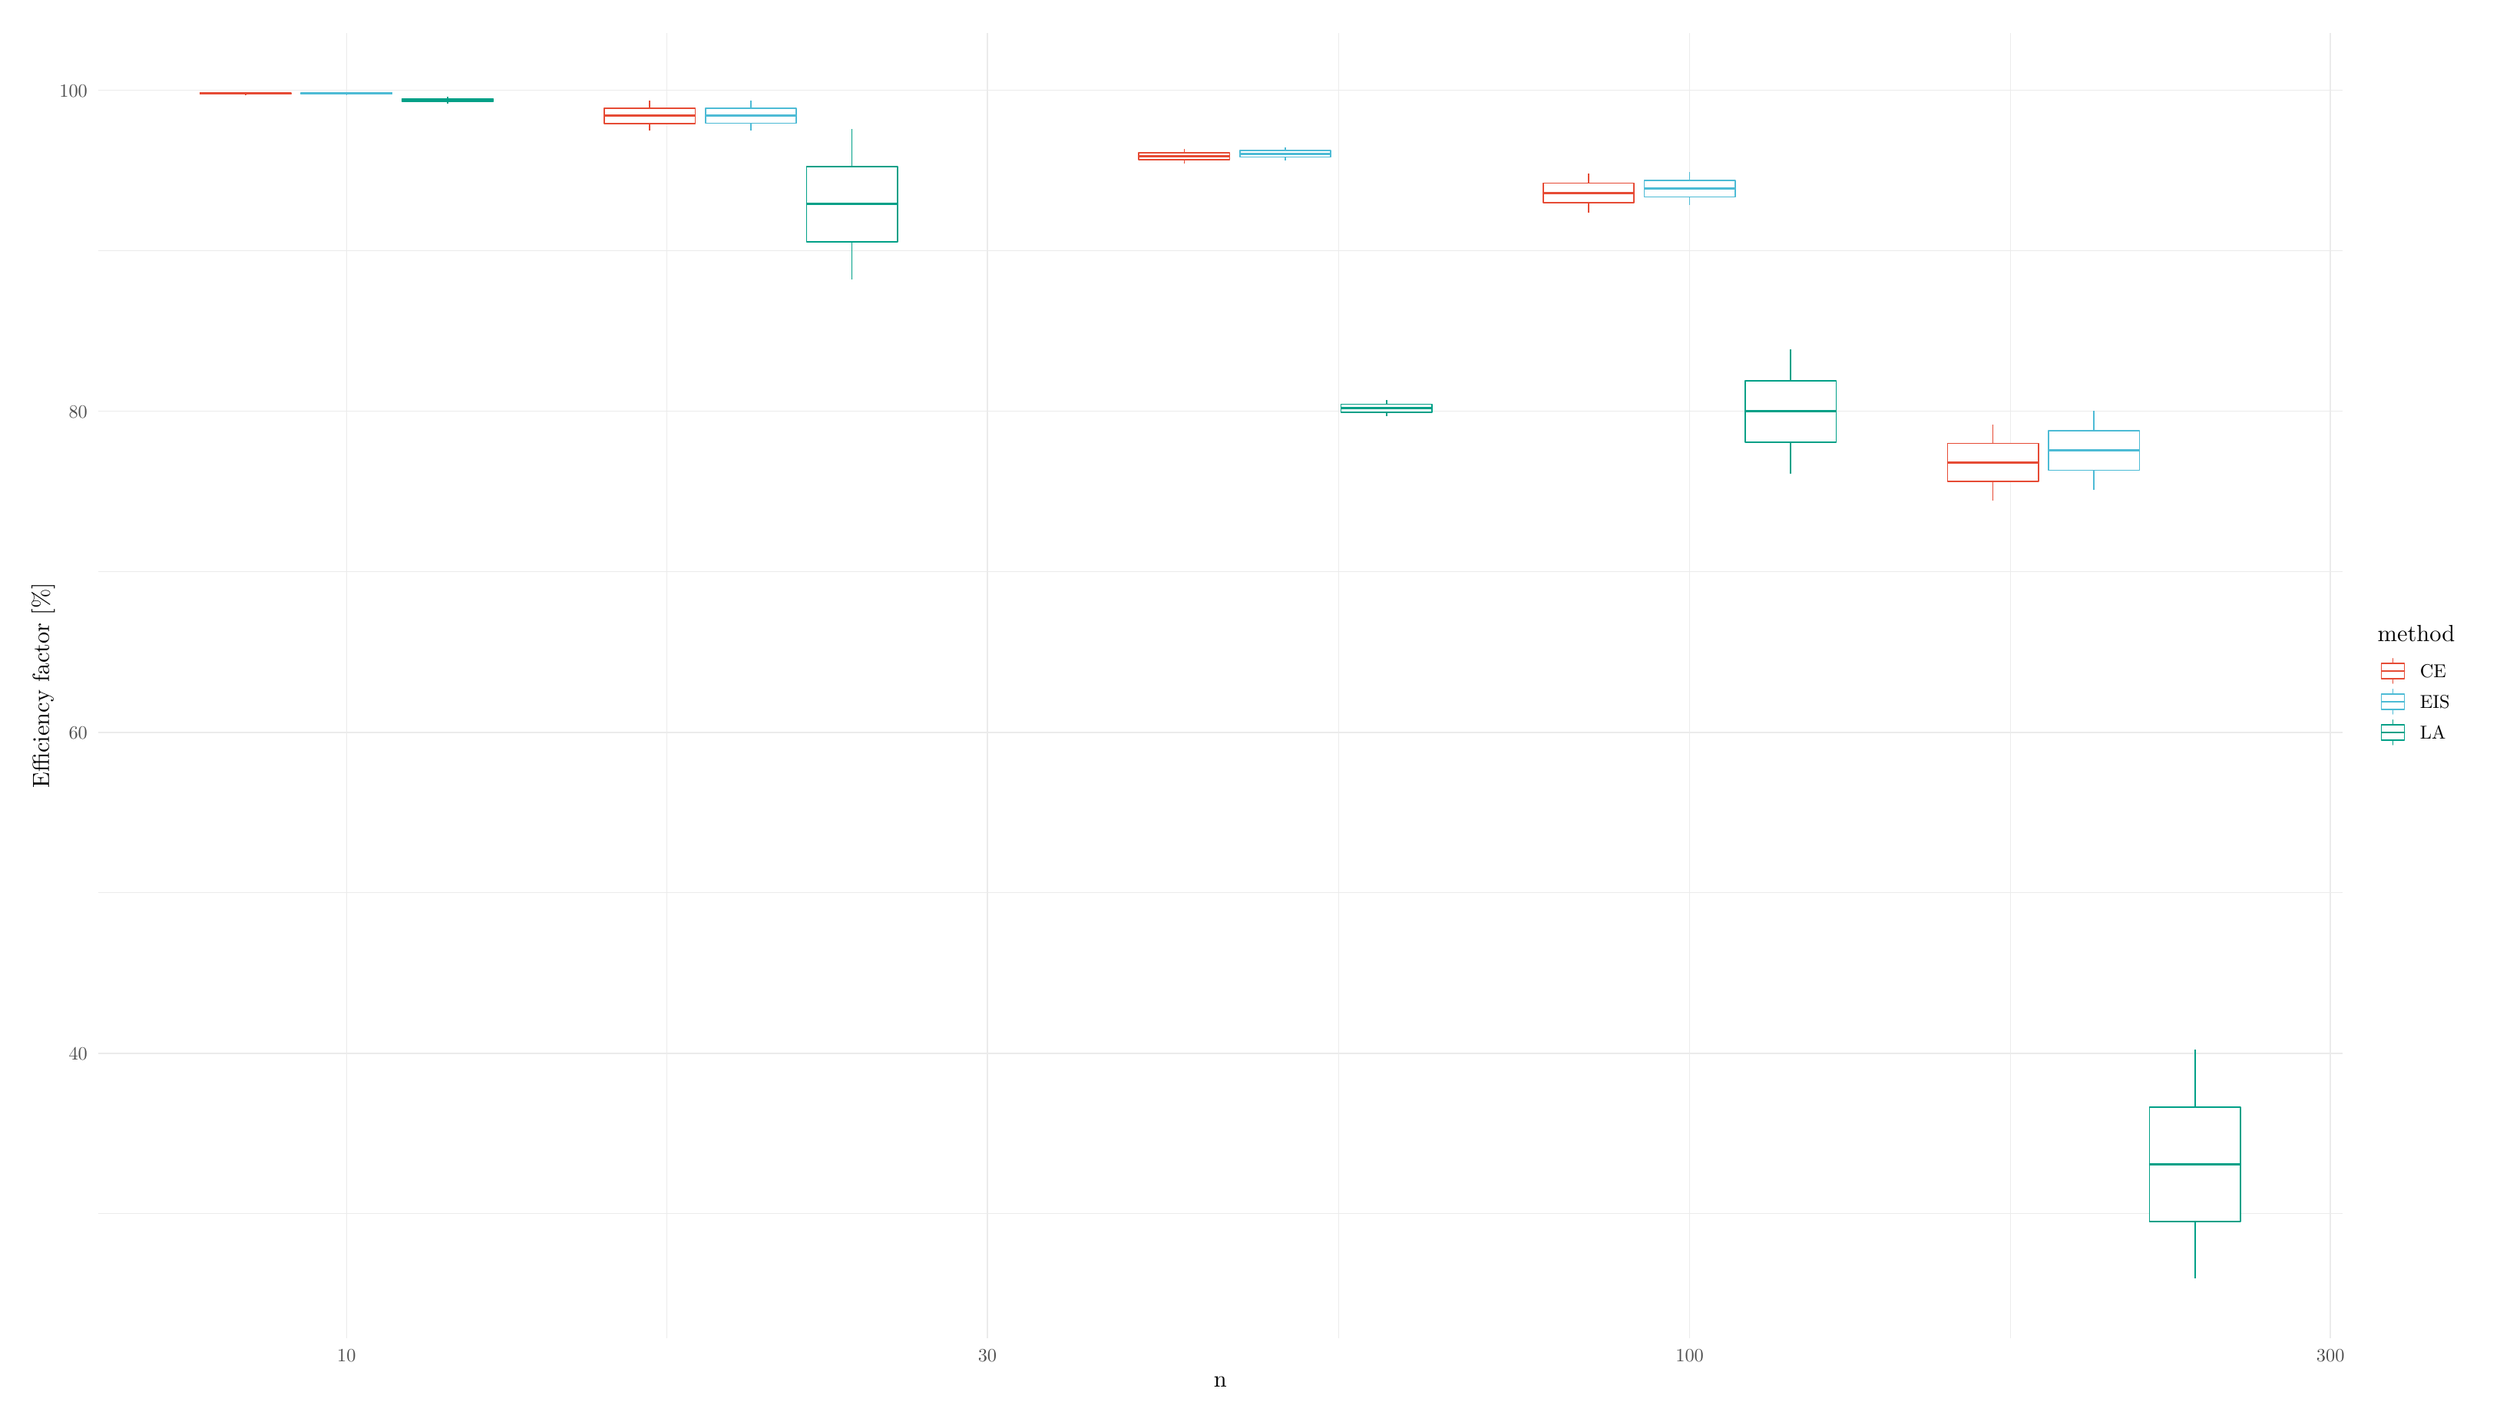
\begin{tikzpicture}[x=1pt,y=1pt]
\definecolor{fillColor}{RGB}{255,255,255}
\path[use as bounding box,fill=fillColor,fill opacity=0.00] (0,0) rectangle (1156.32,650.43);
\begin{scope}
\path[clip] ( 36.11, 30.69) rectangle (1092.47,644.93);
\definecolor{drawColor}{gray}{0.92}

\path[draw=drawColor,line width= 0.3pt,line join=round] ( 36.11, 89.19) --
	(1092.47, 89.19);

\path[draw=drawColor,line width= 0.3pt,line join=round] ( 36.11,240.26) --
	(1092.47,240.26);

\path[draw=drawColor,line width= 0.3pt,line join=round] ( 36.11,391.33) --
	(1092.47,391.33);

\path[draw=drawColor,line width= 0.3pt,line join=round] ( 36.11,542.40) --
	(1092.47,542.40);

\path[draw=drawColor,line width= 0.3pt,line join=round] (303.90, 30.69) --
	(303.90,644.93);

\path[draw=drawColor,line width= 0.3pt,line join=round] (619.94, 30.69) --
	(619.94,644.93);

\path[draw=drawColor,line width= 0.3pt,line join=round] (935.99, 30.69) --
	(935.99,644.93);

\path[draw=drawColor,line width= 0.6pt,line join=round] ( 36.11,164.72) --
	(1092.47,164.72);

\path[draw=drawColor,line width= 0.6pt,line join=round] ( 36.11,315.79) --
	(1092.47,315.79);

\path[draw=drawColor,line width= 0.6pt,line join=round] ( 36.11,466.86) --
	(1092.47,466.86);

\path[draw=drawColor,line width= 0.6pt,line join=round] ( 36.11,617.93) --
	(1092.47,617.93);

\path[draw=drawColor,line width= 0.6pt,line join=round] (153.10, 30.69) --
	(153.10,644.93);

\path[draw=drawColor,line width= 0.6pt,line join=round] (454.69, 30.69) --
	(454.69,644.93);

\path[draw=drawColor,line width= 0.6pt,line join=round] (785.20, 30.69) --
	(785.20,644.93);

\path[draw=drawColor,line width= 0.6pt,line join=round] (1086.78, 30.69) --
	(1086.78,644.93);
\definecolor{drawColor}{RGB}{230,75,53}

\path[draw=drawColor,line width= 0.6pt,line join=round] (105.53,616.69) -- (105.53,616.99);

\path[draw=drawColor,line width= 0.6pt,line join=round] (105.53,616.10) -- (105.53,615.80);
\definecolor{fillColor}{RGB}{255,255,255}

\path[draw=drawColor,line width= 0.6pt,line join=round,line cap=round,fill=fillColor] ( 84.13,616.69) --
	( 84.13,616.10) --
	(126.94,616.10) --
	(126.94,616.69) --
	( 84.13,616.69) --
	cycle;

\path[draw=drawColor,line width= 1.1pt,line join=round] ( 84.13,616.39) -- (126.94,616.39);

\path[draw=drawColor,line width= 0.6pt,line join=round] (295.81,609.43) -- (295.81,612.96);

\path[draw=drawColor,line width= 0.6pt,line join=round] (295.81,602.35) -- (295.81,598.82);

\path[draw=drawColor,line width= 0.6pt,line join=round,line cap=round,fill=fillColor] (274.41,609.43) --
	(274.41,602.35) --
	(317.22,602.35) --
	(317.22,609.43) --
	(274.41,609.43) --
	cycle;

\path[draw=drawColor,line width= 1.1pt,line join=round] (274.41,605.89) -- (317.22,605.89);

\path[draw=drawColor,line width= 0.6pt,line join=round] (547.35,588.56) -- (547.35,590.26);

\path[draw=drawColor,line width= 0.6pt,line join=round] (547.35,585.16) -- (547.35,583.46);

\path[draw=drawColor,line width= 0.6pt,line join=round,line cap=round,fill=fillColor] (525.94,588.56) --
	(525.94,585.16) --
	(568.75,585.16) --
	(568.75,588.56) --
	(525.94,588.56) --
	cycle;

\path[draw=drawColor,line width= 1.1pt,line join=round] (525.94,586.86) -- (568.75,586.86);

\path[draw=drawColor,line width= 0.6pt,line join=round] (737.63,574.25) -- (737.63,578.85);

\path[draw=drawColor,line width= 0.6pt,line join=round] (737.63,565.05) -- (737.63,560.45);

\path[draw=drawColor,line width= 0.6pt,line join=round,line cap=round,fill=fillColor] (716.22,574.25) --
	(716.22,565.05) --
	(759.03,565.05) --
	(759.03,574.25) --
	(716.22,574.25) --
	cycle;

\path[draw=drawColor,line width= 1.1pt,line join=round] (716.22,569.65) -- (759.03,569.65);

\path[draw=drawColor,line width= 0.6pt,line join=round] (927.91,451.78) -- (927.91,460.73);

\path[draw=drawColor,line width= 0.6pt,line join=round] (927.91,433.88) -- (927.91,424.94);

\path[draw=drawColor,line width= 0.6pt,line join=round,line cap=round,fill=fillColor] (906.50,451.78) --
	(906.50,433.88) --
	(949.31,433.88) --
	(949.31,451.78) --
	(906.50,451.78) --
	cycle;

\path[draw=drawColor,line width= 1.1pt,line join=round] (906.50,442.83) -- (949.31,442.83);
\definecolor{drawColor}{RGB}{77,187,213}

\path[draw=drawColor,line width= 0.6pt,line join=round] (153.10,616.72) -- (153.10,617.01);

\path[draw=drawColor,line width= 0.6pt,line join=round] (153.10,616.15) -- (153.10,615.86);

\path[draw=drawColor,line width= 0.6pt,line join=round,line cap=round,fill=fillColor] (131.70,616.72) --
	(131.70,616.15) --
	(174.51,616.15) --
	(174.51,616.72) --
	(131.70,616.72) --
	cycle;

\path[draw=drawColor,line width= 1.1pt,line join=round] (131.70,616.44) -- (174.51,616.44);

\path[draw=drawColor,line width= 0.6pt,line join=round] (343.38,609.50) -- (343.38,613.04);

\path[draw=drawColor,line width= 0.6pt,line join=round] (343.38,602.43) -- (343.38,598.90);

\path[draw=drawColor,line width= 0.6pt,line join=round,line cap=round,fill=fillColor] (321.98,609.50) --
	(321.98,602.43) --
	(364.79,602.43) --
	(364.79,609.50) --
	(321.98,609.50) --
	cycle;

\path[draw=drawColor,line width= 1.1pt,line join=round] (321.98,605.97) -- (364.79,605.97);

\path[draw=drawColor,line width= 0.6pt,line join=round] (594.92,589.52) -- (594.92,591.02);

\path[draw=drawColor,line width= 0.6pt,line join=round] (594.92,586.50) -- (594.92,584.99);

\path[draw=drawColor,line width= 0.6pt,line join=round,line cap=round,fill=fillColor] (573.51,589.52) --
	(573.51,586.50) --
	(616.32,586.50) --
	(616.32,589.52) --
	(573.51,589.52) --
	cycle;

\path[draw=drawColor,line width= 1.1pt,line join=round] (573.51,588.01) -- (616.32,588.01);

\path[draw=drawColor,line width= 0.6pt,line join=round] (785.20,575.56) -- (785.20,579.45);

\path[draw=drawColor,line width= 0.6pt,line join=round] (785.20,567.77) -- (785.20,563.88);

\path[draw=drawColor,line width= 0.6pt,line join=round,line cap=round,fill=fillColor] (763.79,575.56) --
	(763.79,567.77) --
	(806.60,567.77) --
	(806.60,575.56) --
	(763.79,575.56) --
	cycle;

\path[draw=drawColor,line width= 1.1pt,line join=round] (763.79,571.66) -- (806.60,571.66);

\path[draw=drawColor,line width= 0.6pt,line join=round] (975.48,457.70) -- (975.48,467.03);

\path[draw=drawColor,line width= 0.6pt,line join=round] (975.48,439.05) -- (975.48,429.72);

\path[draw=drawColor,line width= 0.6pt,line join=round,line cap=round,fill=fillColor] (954.07,457.70) --
	(954.07,439.05) --
	(996.88,439.05) --
	(996.88,457.70) --
	(954.07,457.70) --
	cycle;

\path[draw=drawColor,line width= 1.1pt,line join=round] (954.07,448.38) -- (996.88,448.38);
\definecolor{drawColor}{RGB}{0,160,135}

\path[draw=drawColor,line width= 0.6pt,line join=round] (200.67,614.00) -- (200.67,614.74);

\path[draw=drawColor,line width= 0.6pt,line join=round] (200.67,612.51) -- (200.67,611.77);

\path[draw=drawColor,line width= 0.6pt,line join=round,line cap=round,fill=fillColor] (179.27,614.00) --
	(179.27,612.51) --
	(222.08,612.51) --
	(222.08,614.00) --
	(179.27,614.00) --
	cycle;

\path[draw=drawColor,line width= 1.1pt,line join=round] (179.27,613.26) -- (222.08,613.26);

\path[draw=drawColor,line width= 0.6pt,line join=round] (390.95,582.03) -- (390.95,599.71);

\path[draw=drawColor,line width= 0.6pt,line join=round] (390.95,546.68) -- (390.95,529.00);

\path[draw=drawColor,line width= 0.6pt,line join=round,line cap=round,fill=fillColor] (369.55,582.03) --
	(369.55,546.68) --
	(412.36,546.68) --
	(412.36,582.03) --
	(369.55,582.03) --
	cycle;

\path[draw=drawColor,line width= 1.1pt,line join=round] (369.55,564.36) -- (412.36,564.36);

\path[draw=drawColor,line width= 0.6pt,line join=round] (642.49,470.16) -- (642.49,472.06);

\path[draw=drawColor,line width= 0.6pt,line join=round] (642.49,466.37) -- (642.49,464.48);

\path[draw=drawColor,line width= 0.6pt,line join=round,line cap=round,fill=fillColor] (621.08,470.16) --
	(621.08,466.37) --
	(663.89,466.37) --
	(663.89,470.16) --
	(621.08,470.16) --
	cycle;

\path[draw=drawColor,line width= 1.1pt,line join=round] (621.08,468.27) -- (663.89,468.27);

\path[draw=drawColor,line width= 0.6pt,line join=round] (832.77,481.29) -- (832.77,495.84);

\path[draw=drawColor,line width= 0.6pt,line join=round] (832.77,452.20) -- (832.77,437.65);

\path[draw=drawColor,line width= 0.6pt,line join=round,line cap=round,fill=fillColor] (811.36,481.29) --
	(811.36,452.20) --
	(854.17,452.20) --
	(854.17,481.29) --
	(811.36,481.29) --
	cycle;

\path[draw=drawColor,line width= 1.1pt,line join=round] (811.36,466.75) -- (854.17,466.75);

\path[draw=drawColor,line width= 0.6pt,line join=round] (1023.04,139.43) -- (1023.04,166.37);

\path[draw=drawColor,line width= 0.6pt,line join=round] (1023.04, 85.55) -- (1023.04, 58.61);

\path[draw=drawColor,line width= 0.6pt,line join=round,line cap=round,fill=fillColor] (1001.64,139.43) --
	(1001.64, 85.55) --
	(1044.45, 85.55) --
	(1044.45,139.43) --
	(1001.64,139.43) --
	cycle;

\path[draw=drawColor,line width= 1.1pt,line join=round] (1001.64,112.49) -- (1044.45,112.49);
\end{scope}
\begin{scope}
\path[clip] (  0.00,  0.00) rectangle (1156.32,650.43);
\definecolor{drawColor}{gray}{0.30}

\node[text=drawColor,anchor=base east,inner sep=0pt, outer sep=0pt, scale=  0.88] at ( 31.16,161.69) {40};

\node[text=drawColor,anchor=base east,inner sep=0pt, outer sep=0pt, scale=  0.88] at ( 31.16,312.76) {60};

\node[text=drawColor,anchor=base east,inner sep=0pt, outer sep=0pt, scale=  0.88] at ( 31.16,463.83) {80};

\node[text=drawColor,anchor=base east,inner sep=0pt, outer sep=0pt, scale=  0.88] at ( 31.16,614.90) {100};
\end{scope}
\begin{scope}
\path[clip] (  0.00,  0.00) rectangle (1156.32,650.43);
\definecolor{drawColor}{gray}{0.30}

\node[text=drawColor,anchor=base,inner sep=0pt, outer sep=0pt, scale=  0.88] at (153.10, 19.68) {10};

\node[text=drawColor,anchor=base,inner sep=0pt, outer sep=0pt, scale=  0.88] at (454.69, 19.68) {30};

\node[text=drawColor,anchor=base,inner sep=0pt, outer sep=0pt, scale=  0.88] at (785.20, 19.68) {100};

\node[text=drawColor,anchor=base,inner sep=0pt, outer sep=0pt, scale=  0.88] at (1086.78, 19.68) {300};
\end{scope}
\begin{scope}
\path[clip] (  0.00,  0.00) rectangle (1156.32,650.43);
\definecolor{drawColor}{RGB}{0,0,0}

\node[text=drawColor,anchor=base,inner sep=0pt, outer sep=0pt, scale=  1.10] at (564.29,  7.64) {n};
\end{scope}
\begin{scope}
\path[clip] (  0.00,  0.00) rectangle (1156.32,650.43);
\definecolor{drawColor}{RGB}{0,0,0}

\node[text=drawColor,rotate= 90.00,anchor=base,inner sep=0pt, outer sep=0pt, scale=  1.10] at ( 13.08,337.81) {Efficiency factor [\%]};
\end{scope}
\begin{scope}
\path[clip] (  0.00,  0.00) rectangle (1156.32,650.43);
\definecolor{drawColor}{RGB}{0,0,0}

\node[text=drawColor,anchor=base west,inner sep=0pt, outer sep=0pt, scale=  1.10] at (1108.97,358.45) {method};
\end{scope}
\begin{scope}
\path[clip] (  0.00,  0.00) rectangle (1156.32,650.43);
\definecolor{drawColor}{RGB}{230,75,53}

\path[draw=drawColor,line width= 0.6pt,line join=round,line cap=round] (1116.19,338.87) --
	(1116.19,341.04);

\path[draw=drawColor,line width= 0.6pt,line join=round,line cap=round] (1116.19,348.27) --
	(1116.19,350.44);
\definecolor{fillColor}{RGB}{255,255,255}

\path[draw=drawColor,line width= 0.6pt,line join=round,line cap=round,fill=fillColor] (1110.77,341.04) rectangle (1121.61,348.27);

\path[draw=drawColor,line width= 0.6pt,line join=round,line cap=round] (1110.77,344.65) --
	(1121.61,344.65);
\end{scope}
\begin{scope}
\path[clip] (  0.00,  0.00) rectangle (1156.32,650.43);
\definecolor{drawColor}{RGB}{77,187,213}

\path[draw=drawColor,line width= 0.6pt,line join=round,line cap=round] (1116.19,324.42) --
	(1116.19,326.59);

\path[draw=drawColor,line width= 0.6pt,line join=round,line cap=round] (1116.19,333.81) --
	(1116.19,335.98);
\definecolor{fillColor}{RGB}{255,255,255}

\path[draw=drawColor,line width= 0.6pt,line join=round,line cap=round,fill=fillColor] (1110.77,326.59) rectangle (1121.61,333.81);

\path[draw=drawColor,line width= 0.6pt,line join=round,line cap=round] (1110.77,330.20) --
	(1121.61,330.20);
\end{scope}
\begin{scope}
\path[clip] (  0.00,  0.00) rectangle (1156.32,650.43);
\definecolor{drawColor}{RGB}{0,160,135}

\path[draw=drawColor,line width= 0.6pt,line join=round,line cap=round] (1116.19,309.97) --
	(1116.19,312.13);

\path[draw=drawColor,line width= 0.6pt,line join=round,line cap=round] (1116.19,319.36) --
	(1116.19,321.53);
\definecolor{fillColor}{RGB}{255,255,255}

\path[draw=drawColor,line width= 0.6pt,line join=round,line cap=round,fill=fillColor] (1110.77,312.13) rectangle (1121.61,319.36);

\path[draw=drawColor,line width= 0.6pt,line join=round,line cap=round] (1110.77,315.75) --
	(1121.61,315.75);
\end{scope}
\begin{scope}
\path[clip] (  0.00,  0.00) rectangle (1156.32,650.43);
\definecolor{drawColor}{RGB}{0,0,0}

\node[text=drawColor,anchor=base west,inner sep=0pt, outer sep=0pt, scale=  0.88] at (1128.92,341.62) {CE};
\end{scope}
\begin{scope}
\path[clip] (  0.00,  0.00) rectangle (1156.32,650.43);
\definecolor{drawColor}{RGB}{0,0,0}

\node[text=drawColor,anchor=base west,inner sep=0pt, outer sep=0pt, scale=  0.88] at (1128.92,327.17) {EIS};
\end{scope}
\begin{scope}
\path[clip] (  0.00,  0.00) rectangle (1156.32,650.43);
\definecolor{drawColor}{RGB}{0,0,0}

\node[text=drawColor,anchor=base west,inner sep=0pt, outer sep=0pt, scale=  0.88] at (1128.92,312.72) {LA};
\end{scope}
\end{tikzpicture}
%
    }
    \caption{The asymptotic efficiency factor degenerates as the number of time steps $n$ increases. We show the estimated efficiency factor over $100$ replications of estimating the optimal parameters for \Cref{ex:negbinom-ar1} with the \gls{cem} and \gls{eis} with $N_{\text{true}} = 10^{6}$ and the resulting estimated efficiency factors at the optimum. Notice the log scale of the x-axis. The performance of the optimal \gls{cem} and \gls{eis} parameters is comparable and superior to that of the \gls{la}}
    \label{fig:ef_time_dimension}
\end{figure}
\section{Conclusion}
\label{sec:03_conclusion}

This chapter provides a comprehensive comparison of the \acrshort{cem} and \acrshort{eis}. Crucially, we provide the \acrshortpl{clt} \Cref{thm:cem-clt,thm:eis-clt} (\Cref{sec:importance_sampling}) and made the \acrshort{cem} feasible for state space models (\Cref{sec:gaussian_importance_sampling_for_state_space_models}). These theoretical insights facilitate the comparisons in \Cref{sec:simulation_studies}, allowing us to bridge the gap between communities that have, to the best of the authors' knowledge, developed separately from one another.

The main insight we can derive from the examples in \Cref{sec:simulation_studies} is that the main obstacle the \acrshort{cem} faces is likely not the fact that its optimal proposal is far away from the target, but rather that its asymptotic variance may be too large to facilitate fast finite-sample convergence. As we have seen in \Cref{subsec:performance_at_optimal}, the efficiency factor at the optimal proposal is --- for most scenarios studied --- comparable between the \acrshort{cem} and \acrshort{eis}. Additionally, in \Cref{fig:cem_eis_sigma2} we saw that \acrshort{eis} tends to produce proposals with larger variances. Following \Cref{lem:gaussian_proposal_factor_2} proposals with larger variance are preferable, as small variance may lead to inadmissible proposals.

Let us stress that the methods we used to obtain the two \acrshortpl{clt} can be applied to other methods that find optimal proposals, such as the \acrshort{vmm} or the recent neural importance sampling \citep{Muller2019Neural}, and can guide choice of importance sampling methods in applications.

In total, we recommend using \acrshort{eis} over the \acrshort{cem} for the following reasons:
\begin{itemize}
    \item the asymptotic variance of \acrshort{eis} seems to be smaller, especially if the target is close to a Gaussian (\Cref{prop:eis-finite-sample}),
    \item \acrshort{eis} is computationally more efficient, as it can be implemented in terms of the efficient simulation smoother and can exploit structure of the linear signal, if it is present and
    \item the least-squares regression is numerically stable and available in many numerical libraries.
\end{itemize}
